% 高一65_大同中学_10月月考.tex
%   —— 高一上数学“2026-2027 年大同中学高一上 10 月月考”（讲评版）
% 试卷版：xelatex 高一65_大同中学_10月月考.tex
% 答案版：xelatex "\def\isanswer{1}% 高一65_大同中学_10月月考.tex
%   —— 高一上数学“2026-2027 年大同中学高一上 10 月月考”（讲评版）
% 试卷版：xelatex 高一65_大同中学_10月月考.tex
% 答案版：xelatex "\def\isanswer{1}% 高一65_大同中学_10月月考.tex
%   —— 高一上数学“2026-2027 年大同中学高一上 10 月月考”（讲评版）
% 试卷版：xelatex 高一65_大同中学_10月月考.tex
% 答案版：xelatex "\def\isanswer{1}% 高一65_大同中学_10月月考.tex
%   —— 高一上数学“2026-2027 年大同中学高一上 10 月月考”（讲评版）
% 试卷版：xelatex 高一65_大同中学_10月月考.tex
% 答案版：xelatex "\def\isanswer{1}\input{高一65_大同中学_10月月考.tex}"
% 紧凑版：xelatex "\def\iscompact{1}\input{高一65_大同中学_10月月考.tex}"
%
% 原始材料：微信公众号“魔都数学加油站”文章，作者破晓，连载“27学年高一65”；
% 原文标题“27学年高一65——2026-2027年上海市大同中学高一上10月月考”；
% 原文链接：https://mp.weixin.qq.com/s/h9ctuk-ByE1Vfg2Rx2C6bw。
% 页面标注发布时间 2026-10-17 21:58（上海）。
% 本次转录只据 `原图/高一65_大同中学_10月月考/` 的 11 张 PNG 逐页读图。
% 正文为 11 张 PNG 页（`01..11.png`）：
% 第 06、11 页 2560×3620，第 01、02、03、04、05、07、08、09、10 页 4762×6735
% （**同一篇各页分辨率不同**），均按页序读取。11 页全为试卷正文页（卷首标题在第 1 页页顶，
% 卷末解答题第 21 题解析止于第 11 页），无封面页、目录页、二维码或宣传页。
% 粉色斜排“魔都数学加油站”为卷面水印，与公众号页脚一并未录入。
%
% 卷首标题：照卷面印作“2026--2027 年大同中学高一上 10 月月考”，年份区间按全稿惯例排 en dash。
% 原卷只有一行标题、无副标题。
%
% 篇幅与题号：原卷自第 3 题起编号（第 1、2 题不在本卷内）。填空题 3—12（10 题）、
% 选择题 13—16（4 题）、解答题 17—21（5 题），共 19 题。本稿沿用原节与原题号，
% 只改排为全稿统一的大节样式（原卷小节标题为“一、填空题”“二、选择题”“三、解答题”）。
%
% 讲评版：原卷每题下直接印【答案】或【解析】。**只印【答案】的 4 题**（第 3、4、7、10 题），
% 本稿只给 \ans{}；其余 15 题都印【解析】（按全稿口径这类题不另提 \ans{}——第 12、13、14、
% 15、16 题的结论写在解析末句（“故选 B”“综上，n 的最大值为 14”等），亦照录在解析内）。
% 全卷无“答案印在题干括号内”的题（第 13—16 题的选择题括号内均空白）。
%
% 副标题：原卷未印副标题。本稿按“知识模块”口径标作“集合与常用逻辑用语、不等式”：
% 19 题中集合与常用逻辑用语 10 题（第 3、4、6、8、12、14、15、18、19、21 题），
% 不等式 9 题（含等式恒等、不等式性质、二次不等式、恒成立、基本不等式、不等式的证明：
% 第 5、7、9、10、11、13、16、17、20 题），两类均超过三分之一，故并标。口径同 高一63。
%
% 与原卷的排版差异：
%   ① 原卷每题下直接印【答案】/【解析】，本稿按全稿惯例将答案与解析置于答案版，试卷版保持干净；
%   ② 原卷未印副标题，本稿按“知识模块”口径补出；
%   ③ 原卷填空横线约四个字宽，本稿按全稿惯例统一排 \blankline[4.4em]；
%   ④ 原卷数集记号全为斜体：实数集作 $R$（第 6 题两处、第 8 题两处、第 15 题解析、第 18 题、
%      第 20 题题干），自然数集作 $N$（第 12 题题干“$n\in N,n\geqslant1$”），有理数集作 $Q$
%      （第 21 题 (2) 题干与解析共 4 处），本稿按全稿惯例统一改用 $\R$、$\N$、$\Q$
%      （同 高一63 排版差异④：记号归一）；空集记号原卷作 $\varnothing$，照录；
%   ⑤ 原卷用描述法时竖线排细竖“$|$”（如 $\{x|0<x<3\}$、$\{x|(x-1)(x-m)<0\}$），
%      本稿按全稿惯例排 \mid；
%   ⑥ 原卷判别式印作“$\triangle$”（第 8、14 题解析各 1 处、第 20 题解析 2 处，共 4 处），
%      本稿照录用 \triangle（同 高一39 成例），未改作 \Delta；
%   ⑦ 第 18—21 题的子问原卷各自另起一行、以“（1）”“（2）”标号，本稿按全稿惯例用
%      enumerate 的 (1)(2)(3)；解析中的子问标号一律用 \stepm{(1)}{…}；
%      第 18—21 题解析（原文以“（1）”“（2）”“（3）”冠于解析首句）同此；
%   ⑧ 选择题的作答括号原卷排半角“(　　)”（第 13—16 题括号内均空白），
%      本稿按全稿惯例排 \mbox{（\quad）}；选项字母后的句点照原卷排“A.”“B.”；
%   ⑨ 每道解答题原卷未留作答空白，本稿按全稿惯例加 \ansspace（末题用 \ansspace*）；
%   ⑩ 原卷在数学式内多处用半角逗号（如 $\{x|0<x<3\},B=\{x|x>2\}$、$m\in I_{14},k\in I_{14}$），
%      均照录未强改；句末句点按全稿惯例排西文句点。
%
% 原卷笔误/存疑（均照录未改，正文对应处另有 % 注）：
%   ① 第 13 题题干“下列不等式中一定成立是（　　）”脱一个“的”（当作“一定成立的是”），
%      8 倍放大确认非水印遮挡，本稿照录；
%   ② 第 15 题【解析】末段把题干条件“$x\geqslant10$”写成“$x\geqslant1$”
%      （“所以 $x+2+\frac{16}{x+2}(x\geqslant1)$ 的最小值不为 8”），与同段前面“令 $t=x+2$，
%      则 $t\geqslant12$”不合，本稿照录；
%   ③ 第 19 题题干把命题 $P$ 印作“$\exists3\notin A$”（多一个存在量词），而【解析】两处
%      均作“$3\notin A$”，前后记号不一，本稿照录；
%   ④ 第 20 题【解析】(2) 出现 $f(|x|)$，但题干只给“函数 $y=ax^2-(a+2)x+2$”、全卷未设 $f$，
%      本稿照录；
%   ⑤ 第 20 题 (2) 题干末句作“求实数 $a$ 的取值”（疑脱“范围”二字），本稿照录；
%   ⑥ 第 12 题【解析】第 18 步“它与 $P_n$ 中的任何其他数之和都不是整数”，该段所论为 $P_{14}$
%      （前后均作 $P_{14}$），此处 $P_n$ 疑当作 $P_{14}$，本稿照录。
%
% 第二轮复核（2026-10-18）订正「本稿抄错原卷」一处：
%   第 21 题 (1)【解析】原卷本作“$\{\{1,2\},\{3\}\}$、$\{\{1,3\},\{2\}\}$、$\{\{2,3\},\{1\}\}$”，
%   有外层花括号；首轮误脱外层花括号，并曾在文件头误记为“原卷未加外层花括号”（原第 ⑦ 条，
%   已撤销）。本次照原卷补回，正文对应处另有 % 注。
%
% 插图：第 16 题【解析】内有 1 幅图（两条开口向上的抛物线 $f(x)$、$g(x)$ 与 $x$ 轴交点
% 标 $a$、$x_1$、$x_2$、$b$，纵轴标 $y$、原点 $O$），解析第三行“画出函数 $g(x)$ 与函数 $f(x)$
% 的图像，如图所示”即指此图；取原卷截图（06.png，2560×3620）右半幅，4× LANCZOS 放大，
% 存 figures/parabola_f_g_x1x2_h65.png。该图在【解析】内，仅答案版出。
%
\documentclass[a4paper,11pt]{article}
\usepackage{common}

\begin{document}

\examtitlest[3]{2026--2027 年大同中学高一上 10 月月考}{集合与常用逻辑用语、不等式}

\bigsec{一、填空题}

\begin{enumerate}
\setcounter{enumi}{2}

\item 已知集合 $A=\{x\mid0<x<3\}$,$B=\{x\mid x>2\}$，则集合 $A\cup B=$\blankline[4.4em].

\ifanswer
\ans{$(0,+\infty)$}
\fi

\item “$x>1$ 或 $y>1$”的否定形式是\blankline[4.4em].

\ifanswer
\ans{$x\leqslant1$ 且 $y\leqslant1$}
\fi

\item 已知等式 $2x^2+3x+4=a(2x+1)(x+1)+b$ 恒成立，则常数 $a-b=$\blankline[4.4em].

\ifanswer
\solbegin
\step{因为等式 $2x^2+3x+4=a(2x+1)(x+1)+b$ 恒成立，}
\step{所以 $a(2x+1)(x+1)+b=2ax^2+3ax+a+b=2x^2+3x+4$，}
\step{所以 $\begin{cases}2a=2\\ 3a=3\\ a+b=4\end{cases}$，解得 $\begin{cases}a=1\\ b=3\end{cases}$，所以 $a-b=-2$.}
\solend
\fi

\item 全集为 $U=\R$，$A=\{x\mid|x|\geqslant2\}$，$B=\{y\mid y=x^2+1,x\in\R\}$，则 $A\cup\bar B=$\blankline[4.4em].

\ifanswer
\solbegin
\step{由题意得集合 $A=\{x\mid x\geqslant2\text{ 或 }x\leqslant-2\}$，}
\step{因为 $x^2+1\geqslant1$，所以集合 $B=\{x\mid x\geqslant1\}$，所以 $\bar B=\{x\mid x<1\}$，}
\step{则 $A\cup\bar B=\{x\mid x\geqslant2\text{ 或 }x<1\}$.}
\solend
\fi

\item 已知 $|x+3|+|x-5|=8$，则实数 $x$ 的取值范围为\blankline[4.4em].

\ifanswer
\ans{$[-3,5]$}
\fi

\item 已知集合 $A=\{x\in\R\mid ax^2+2x+1=0,a\in\R\}$ 只有一个元素，则 $a$ 的值为\blankline[4.4em].

\ifanswer
\solbegin
\step{当 $a=0$ 时，$A=\left\{-\dfrac12\right\}$；}
\step{当 $a\neq0$ 时，若集合 $A$ 只有一个元素，由 $\triangle=4-4a=0$ 得 $a=1$.}
\step{综上，当 $a=0$ 或 $a=1$ 时，集合 $A$ 只有一个元素.}
\solend
\fi

\item 已知不等式 $-x^2+bx+c>0$ 的解集为 $(3,4)$，则不等式 $cx^2+bx-1<0$ 的解集为\blankline[4.4em].

\ifanswer
\solbegin
\step{由题意得 3，4 是方程 $-x^2+bx+c=0$ 的两个实数根，}
\step{所以 $\begin{cases}3+4=b\\ 3\times4=-c\end{cases}$，得 $b=7$，$c=-12$，}
\step{则不等式 $cx^2+bx-1<0$，即为 $-12x^2+7x-1<0$，即 $12x^2-7x+1>0$，}
\step{化简得 $(3x-1)(4x-1)>0$，解得 $x<\dfrac14$ 或 $x>\dfrac13$，}
\step{即不等式 $cx^2+bx-1<0$ 的解集为 $\left(-\infty,\dfrac14\right)\cup\left(\dfrac13,+\infty\right)$.}
\solend
\fi

\item 对于区间 $(m,n)$，我们将 $n-m$ 的值称为该区间的长度. 若关于 $x$ 的不等式
$x^2+ax+a<0$ 有解，且解集的区间长度不超过 $2\sqrt3$，则实数 $a$ 的取值范围是\blankline[4.4em].

\ifanswer
\ans{$[-2,0)\cup(4,6]$}
\fi

\item 当 $x>0$ 时，关于 $x$ 的不等式 $(ax-1)(x^2+bx-4)\geqslant0$ 恒成立，则 $b+\dfrac2a$ 的最小值
为\blankline[4.4em].

\ifanswer
\solbegin
\step{由题意 $a\neq0$；}
\step{若 $a<0$，则 $x>0$ 时 $ax-1<0$ 恒成立，需 $x^2+bx-4\leqslant0$ 对一切 $x>0$ 成立，}
\step{而 $y=x^2+bx-4$ 的图象开口向上，当 $x$ 充分大时必为正值，矛盾，故 $a>0$.}
\step{当 $a>0$ 时，$ax-1=a\left(x-\dfrac1a\right)$，故原条件化为 $\left(x-\dfrac1a\right)(x^2+bx-4)\geqslant0$：}
\step{若 $0<x<\dfrac1a$，则 $x-\dfrac1a<0$，需 $x^2+bx-4\leqslant0$；}
\step{若 $x>\dfrac1a$，则 $x-\dfrac1a>0$，需 $x^2+bx-4\geqslant0$；}
\step{由 $y=x^2+bx-4$ 的连续性知 $x=\dfrac1a$ 是它的零点，}
\step{即 $\dfrac1{a^2}+\dfrac ba-4=0$，得 $b=4a-\dfrac1a$；}
\step{此时 $x^2+bx-4=x^2+\left(4a-\dfrac1a\right)x-4=(x+4a)\left(x-\dfrac1a\right)$，}
\step{由 $a>0$、$x>0$ 得 $x+4a>0$，}
\step{其符号与 $x-\dfrac1a$ 一致，故能与 $ax-1$ 同号，原不等式确在 $x>0$ 上恒成立.}
\step{于是 $b+\dfrac2a=4a-\dfrac1a+\dfrac2a=4a+\dfrac1a\geqslant2\sqrt{4a\cdot\dfrac1a}=4$，}
\step{当且仅当 $a=\dfrac12$ 时取等号，故最小值为 4.}
\solend
\fi

\item 设集合 $I_n=\{1,2,\cdots,n\}$，$n\in\N$，$n\geqslant1$，集合 $P_n=\left\{\dfrac m{\sqrt k}\mid m\in I_n,k\in I_n\right\}$，若 $P_n$ 的子集 $A$
中任意两个元素之和不是整数的平方，则称 $A$ 为“人文集”. 那么使 $P_n$ 能分成两个交集为空
集的“人文集”的并集，且这两个人文集的并集恰为 $P_n$ 时，$n$ 的最大值是\blankline[4.4em].

\ifanswer
\solbegin
\step{先证当 $n\geqslant15$ 时，$P_n$ 不能分成两个不相交的人文集的并集.}
\step{假设当 $n\geqslant15$ 时，$P_n$ 可以分成两个不相交的人文集的并集，}
\step{设 $A$ 和 $B$ 为两个不相交的人文集，使 $A\cup B=P_n\supseteq I_n$.}
\step{不妨设 $1\in A$，则由于 $1+3=2^2$，所以 $3\notin A$，即 $3\in B$.}
\step{同理可得，$6\in A$，$10\in B$. 又推出 $15\in A$，}
\step{但 $1+15=4^2$，这与 $A$ 为人文集相矛盾.}
\step{再证 $P_{14}$ 满足要求. 当 $k=1$ 时，$P_{14}=\left\{\dfrac m{\sqrt k}\mid m\in I_{14},k\in I_{14}\right\}$，}
\step{可以分成 2 个人文集的并集.}
\step{事实上，只要取 $A_1=\{1,2,4,6,9,11,13\}$，$B_1=\{3,5,7,8,10,12,14\}$，}
\step{则 $A_1$ 和 $B_1$ 都是人文集，且 $A_1\cup B_1=P_{14}$.}
\step{当 $k=4$ 时，集合 $\left\{\dfrac m{\sqrt k}\mid m\in I_{14}\right\}$ 中，除整数外，}
\step{剩下的数组成集合 $\left\{\dfrac12,\dfrac32,\dfrac52,\cdots,\dfrac{13}2\right\}$，}
\step{可以分为下列 2 个人文集的并：$A_2=\left\{\dfrac12,\dfrac52,\dfrac92,\dfrac{11}2\right\}$，$B_2=\left\{\dfrac32,\dfrac72,\dfrac{13}2\right\}$.}
\step{当 $k=9$ 时，集合 $\left\{\dfrac m{\sqrt k}\mid m\in I_{14}\right\}$ 中，除整数外，}
\step{剩下的数组成集合 $\left\{\dfrac13,\dfrac23,\dfrac43,\dfrac53,\cdots,\dfrac{13}3,\dfrac{14}3\right\}$，}
\step{可以分为下列 2 个人文集的并：$A_3=\left\{\dfrac13,\dfrac43,\dfrac53,\dfrac{10}3,\dfrac{13}3\right\}$，$B_3=\left\{\dfrac23,\dfrac73,\dfrac83,\dfrac{11}3,\dfrac{14}3\right\}$.}
\step{最后，集合 $C=\left\{\dfrac m{\sqrt k}\mid m\in I_{14},k\in I_{14},k\neq1,4,9\right\}$ 中的数的分母都是无理数，}
% 注：本行原卷作“$P_n$”，而该段所论为 $P_{14}$（前后均作 $P_{14}$），疑当作 $P_{14}$；
%     照录未改，见文件头“原卷笔误/存疑”⑥。
\step{它与 $P_n$ 中的任何其他数之和都不是整数，}
\step{因此，令 $A=A_1\cup A_2\cup A_3\cup C$，$B=B_1\cup B_2\cup B_3$，}
\step{则 $A$ 和 $B$ 是不相交的人文集，且 $A\cup B=P_{14}$.}
\step{综上，$n$ 的最大值为 14.}
\solend
\fi

\end{enumerate}

\bigsec{二、选择题}

\begin{enumerate}
\setcounter{enumi}{12}

% 注：原卷题干“下列不等式中一定成立是”脱一个“的”（当作“一定成立的是”），
%     照录未改，见文件头“原卷笔误/存疑”①。
\item 已知 $a>b$，下列不等式中一定成立是\mbox{（\quad）}

\keepwithprev
A. $a^2>b^2$\qquad B. $ac^2>bc^2$\qquad C. $\dfrac1a<\dfrac1b$\qquad D. $a+3>b-4$

\ifanswer
\solbegin
\step{对于 $A$，当 $a=-2$，$b=-4$ 时，不等式不成立，故 $A$ 错误；}
\step{对于 $B$，当 $c=0$ 时，不等式不成立，故 $B$ 错误；}
\step{对于 $C$，当 $a=2$，$b=-4$ 时，不等式不成立，故 $C$ 错误；}
\step{对于 $D$，因为 $a>b$，$3>-4$，必有 $a+3>b-4$ 成立，故 $D$ 正确.}
\step{故选 $D$.}
\solend
\fi

\item 已知 $a$ 为实数，那么“$|a|\leqslant2$”是“方程 $x^2+ax+1=0$ 没有实数解”的\mbox{（\quad）}

\keepwithprev
A. 充分而不必要条件\qquad B. 必要而不充分条件

C. 充要条件\qquad D. 既不充分也不必要条件

\ifanswer
\solbegin
\step{由方程 $x^2+ax+1=0$ 没有实数解，得 $\triangle=a^2-4<0$，则 $|a|<2$，}
\step{由 $|a|<2$ 得 $|a|\leqslant2$，反之不成立，}
\step{所以“$|a|\leqslant2$”是“方程 $x^2+ax+1=0$ 没有实数解”的必要而不充分条件.}
\step{故选 $B$.}
\solend
\fi

\item 下列命题为真命题的是\mbox{（\quad）}

\keepwithprev
A. $a>b>0$，当 $m>0$ 时，$\dfrac{a+m}{b+m}>\dfrac ab$

B. 集合 $A=\{x\mid y=x^2+1\}$ 与集合 $B=\{y\mid y=x^2+1\}$ 是相同的集合

C. 若 $b<a<0$，$m<0$，则 $\dfrac ma>\dfrac mb$

D. $x+2+\dfrac{16}{x+2}(x\geqslant10)$ 最小值为 8

\ifanswer
\solbegin
\step{对于 $A$，$\dfrac{a+m}{b+m}-\dfrac ab=\dfrac{b(a+m)-a(b+m)}{b(b+m)}=\dfrac{m(b-a)}{b(b+m)}$，}
\step{因为 $a>b>0$，$m>0$，所以 $b(b+m)>0$，$m(b-a)<0$，}
\step{所以 $\dfrac{a+m}{b+m}-\dfrac ab=\dfrac{m(b-a)}{b(b+m)}<0$，}
\step{即 $a>b>0$，当 $m>0$ 时，$\dfrac{a+m}{b+m}<\dfrac ab$，故 $A$ 错误；}
\step{对于 $B$，集合 $A=\{x\mid y=x^2+1\}=\R$，集合 $B=\{y\mid y=x^2+1\}=\{y\mid y\geqslant1\}$，}
\step{所以 $A\neq B$，故 $B$ 错误；}
\step{对于 $C$，$\dfrac ma-\dfrac mb=\dfrac{m(b-a)}{ab}$，}
\step{因为 $b<a<0$，$m<0$，所以 $ab>0$，$m(b-a)>0$，}
\step{所以 $\dfrac ma-\dfrac mb=\dfrac{m(b-a)}{ab}>0$，即 $\dfrac ma>\dfrac mb$，故 $C$ 正确；}
\step{对于 $D$，令 $t=x+2$，则 $t\geqslant12$，表达式变为 $t+\dfrac{16}t$，}
\step{$t+\dfrac{16}t\geqslant2\sqrt{t\cdot\dfrac{16}t}=8$，当且仅当 $t=4$ 时取等号，即等号不成立，}
% 注：原卷本行把题干条件“$x\geqslant10$”写成“$x\geqslant1$”，与同段“$t\geqslant12$”不合；
%     照录未改，见文件头“原卷笔误/存疑”②。
\step{所以 $x+2+\dfrac{16}{x+2}(x\geqslant1)$ 的最小值不为 8，故 $D$ 错误.}
\step{故选 $C$.}
\solend
\fi

\item 已知实数 $a<b$，关于 $x$ 的不等式 $x^2-(a+b)x+ab+\dfrac12<0$ 的解集为 $(x_1,x_2)$，则实数 $a$、
$b$、$x_1$、$x_2$ 从小到大的排列是\mbox{（\quad）}

\keepwithprev
A. $x_1<a<b<x_2$\qquad B. $a<x_1<x_2<b$\qquad C. $a<x_1<b<x_2$\qquad D. $x_1<a<x_2<b$

\ifanswer
\solbegin
\step{不等式 $x^2-(a+b)x+ab+\dfrac12<0$ 可化为 $(x-a)(x-b)+\dfrac12<0$，}
\step{设 $g(x)=(x-a)(x-b)$，$f(x)=g(x)+\dfrac12$，}
\step{画出函数 $g(x)$ 与函数 $f(x)$ 的图像，如图所示，}
% 图在【解析】内（仅答案版出），取原卷截图（06.png，2560×3620）右半幅，4× LANCZOS 放大。
\begin{center}
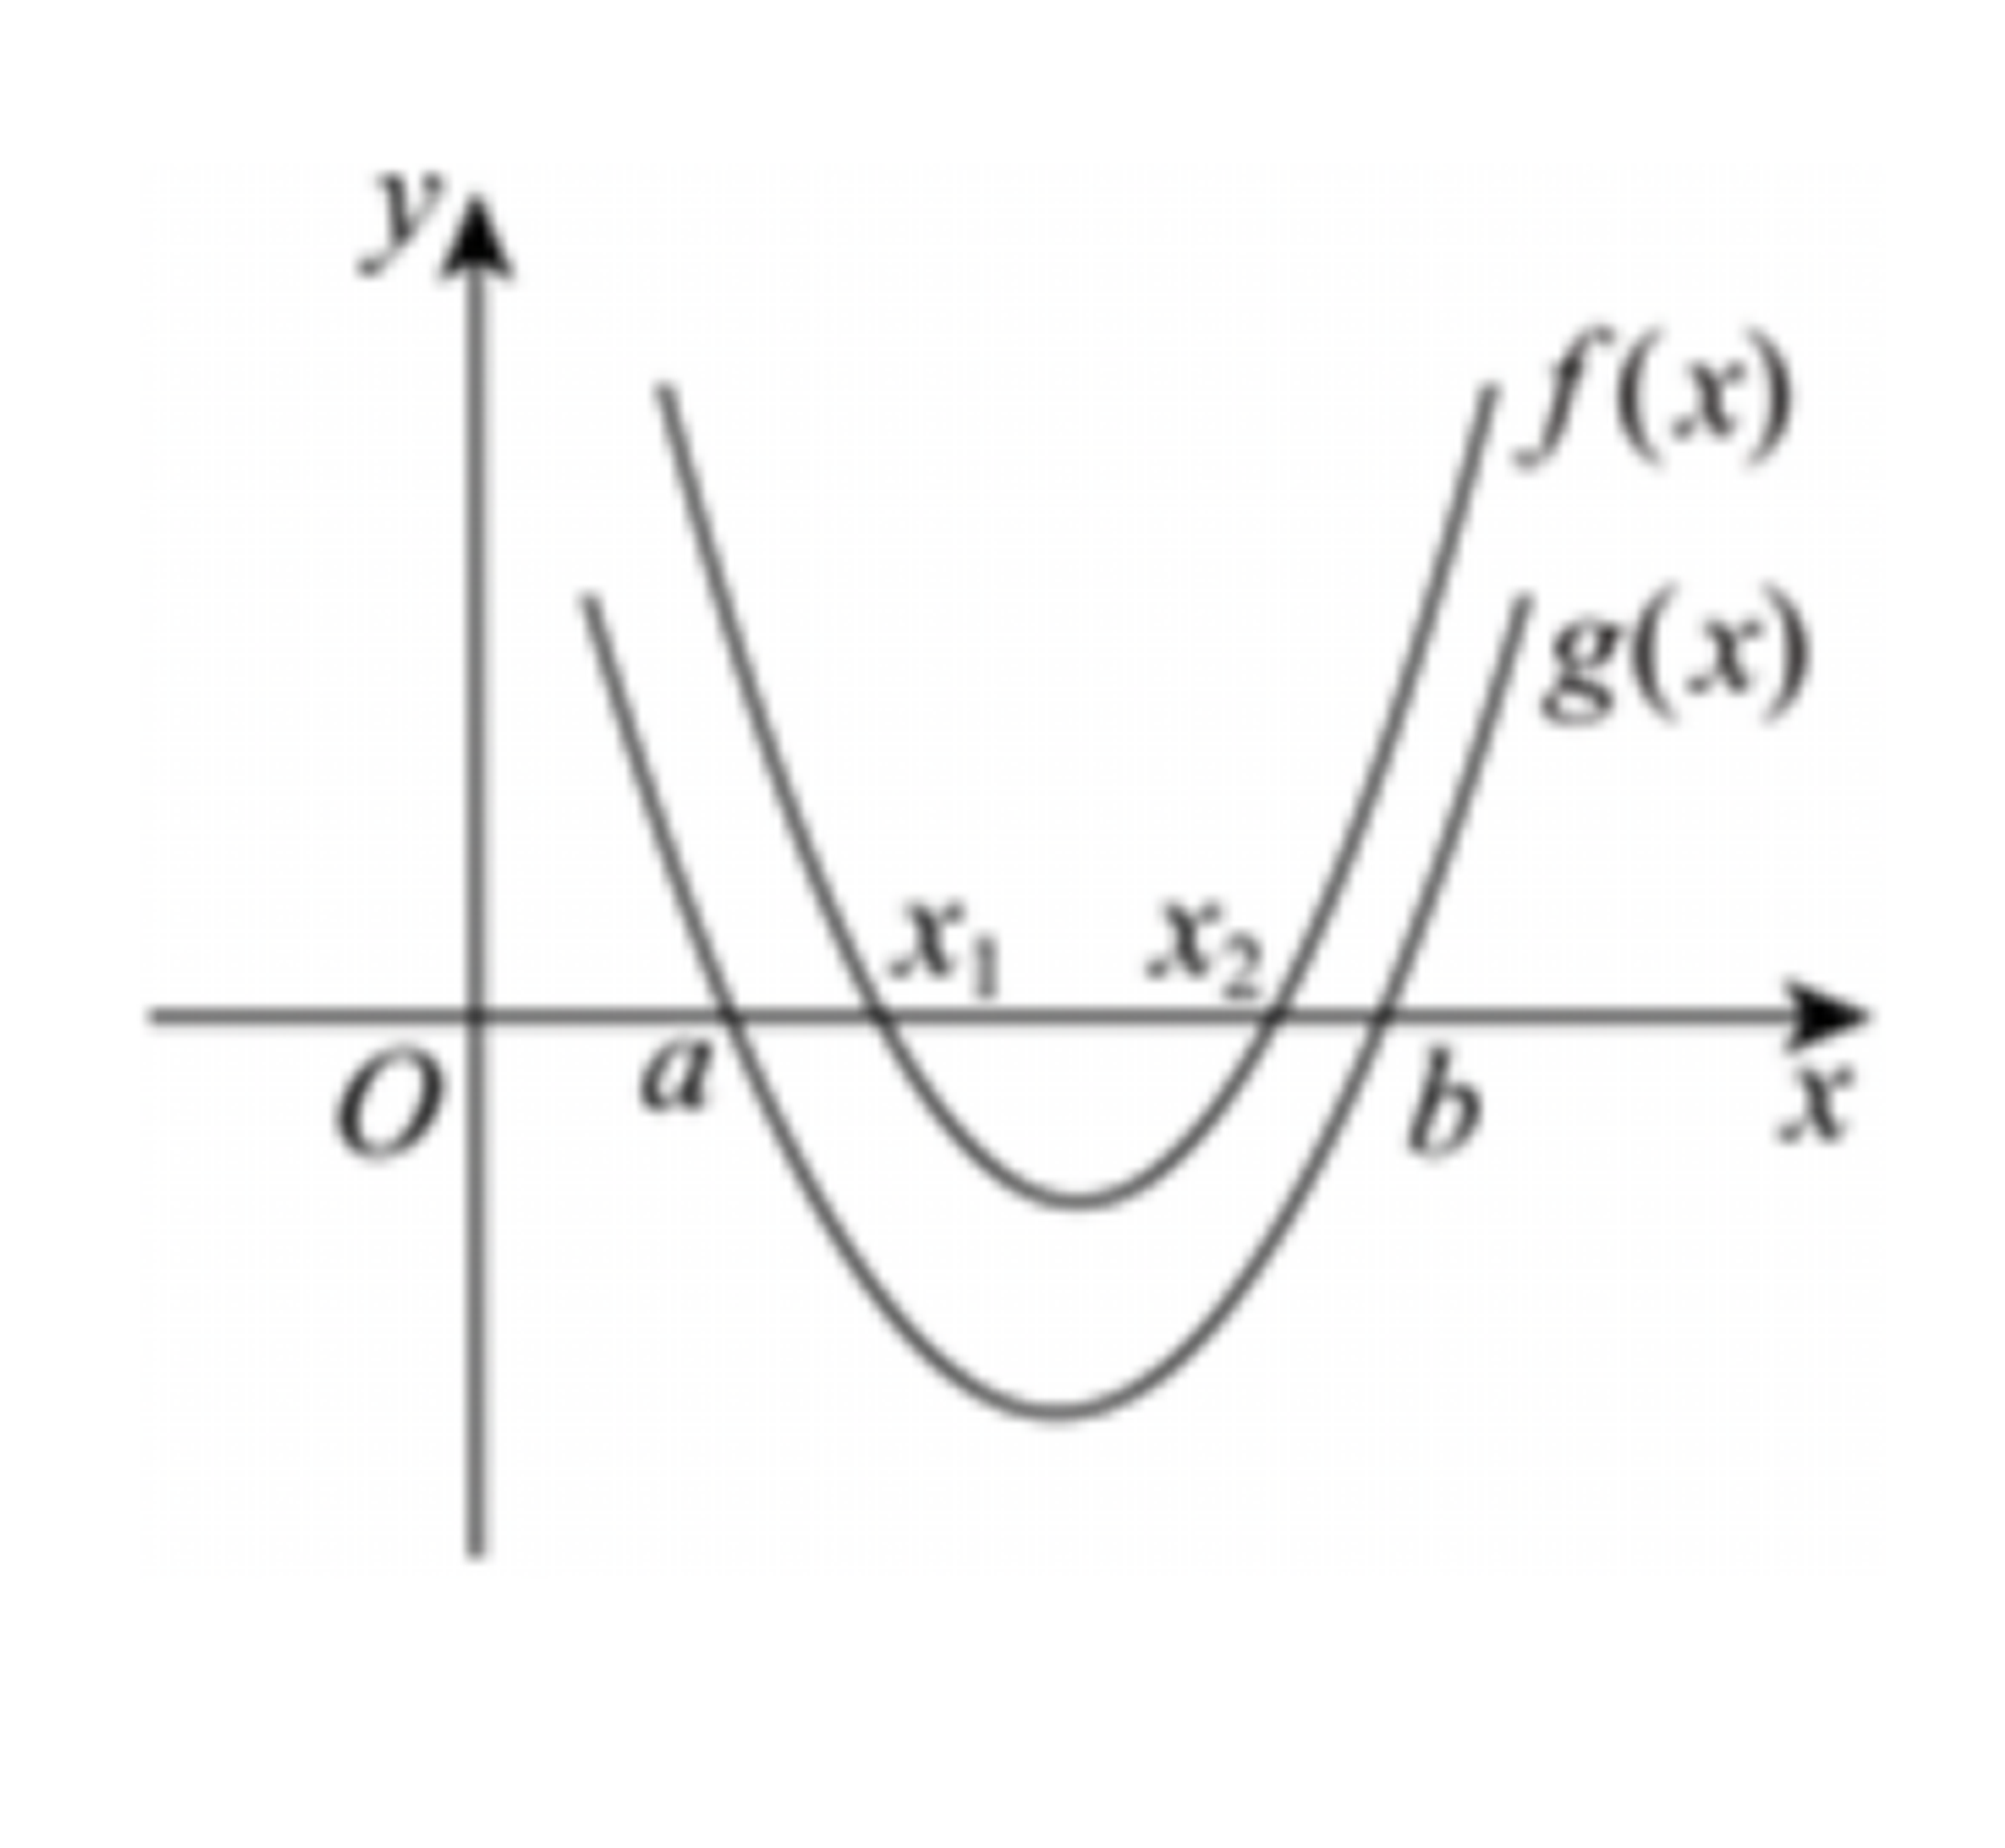
\includegraphics[width=0.30\textwidth]{figures/parabola_f_g_x1x2_h65.png}
\end{center}
\step{由图像得 $a<x_1<x_2<b$，故选 $B$.}
\solend
\fi

\end{enumerate}

\bigsec{三、解答题}

\begin{enumerate}
\setcounter{enumi}{16}

\item 已知 $a>0$，$b>0$，若 $a+b>4$，求证：$\dfrac a{b+2}$ 和 $\dfrac b{a+2}$ 中至少有一个大于 $\dfrac12$.

\ifanswer
\solbegin
\step{假设 $\dfrac a{b+2}\leqslant\dfrac12$，$\dfrac b{a+2}\leqslant\dfrac12$，}
\step{$a>0$，$b>0$，则 $a+2>0$，$b+2>0$，故 $2a\leqslant b+2$，$2b\leqslant a+2$，}
\step{两式相加得 $a+b\leqslant4$，与 $a+b>4$ 矛盾，故 $\dfrac a{b+2}$ 和 $\dfrac b{a+2}$ 中至少有一个大于 $\dfrac12$.}
\solend
\fi

\ansspace[6]

\item 已知集合 $A=\{x\mid-4<x<5\}$，$B=\{x\mid x\leqslant a-6\text{ 或 }x\geqslant a+2\}$.

\begin{enumerate}[label=(\arabic*)]

\item 若 $A\cup B=\R$，求实数 $a$ 的取值范围；

\item 若“$x\in A$”是“$x\in B$”的充分不必要条件，求实数 $a$ 的取值范围.

\end{enumerate}

\ifanswer
\solbegin
\stepm{(1)}{集合 $A=\{x\mid-4<x<5\}$，$B=\{x\mid x\leqslant a-6\text{ 或 }x\geqslant a+2\}$.}
\step{由 $A\cup B=\R$ 得 $\begin{cases}a-6\geqslant-4\\ a+2\leqslant5\end{cases}$，解得 $2\leqslant a\leqslant3$，$a$ 的取值范围为 $[2,3]$；}
\stepm{(2)}{若“$x\in A$”是“$x\in B$”的充分不必要条件，则 $A\subset B$，}
\step{则 $5\leqslant a-6$ 或 $-4\geqslant a+2$，解得 $a\leqslant-6$ 或 $a\geqslant11$.}
\solend
\fi

\ansspace[8]

% 注：原卷题干把命题 $P$ 印作“$\exists3\notin A$”（多一个存在量词），而【解析】两处均作
%     “$3\notin A$”；照录未改，见文件头“原卷笔误/存疑”③。
\item 已知集合 $A=\left\{x\mid\dfrac{x-1}{x-m}<0\right\}$，集合 $B=\left\{x\mid\left|\dfrac{x-1}{x-3}\right|\geqslant1\right\}$，命题 $P$：“$\exists3\notin A$”，命题
$Q$：$A\cap B\neq\varnothing$.

\begin{enumerate}[label=(\arabic*)]

\item 若命题 $P$ 为真命题，求 $m$ 的取值范围；

\item 若命题 $P$ 和命题 $Q$ 至少有一个为假命题，求实数 $m$ 的取值范围.

\end{enumerate}

\ifanswer
\solbegin
\stepm{(1)}{$A=\left\{x\mid\dfrac{x-1}{x-m}<0\right\}=\{x\mid(x-1)(x-m)<0\}$，}
\step{若命题 $P$：“$3\notin A$”为真命题，则 $(3-1)(3-m)\geqslant0$，解得 $m\leqslant3$，}
\step{故实数 $m$ 的取值范围为 $(-\infty,3]$；}
\stepm{(2)}{$B=\left\{x\mid\left|\dfrac{x-1}{x-3}\right|\geqslant1\right\}$，由 $\left|\dfrac{x-1}{x-3}\right|\geqslant1$，得 $\begin{cases}|x-1|\geqslant|x-3|\\ x\neq3\end{cases}$，}
\step{等价于 $\begin{cases}(x-1)^2\geqslant(x-3)^2\\ x\neq3\end{cases}$，解得 $x\geqslant2$ 且 $x\neq3$，所以 $B=[2,3)\cup(3,+\infty)$，}
\step{因为 $A=\{x\mid(x-1)(x-m)<0\}$，}
\step{当 $m=1$ 时，$A=\varnothing$，不满足 $A\cap B\neq\varnothing$，}
\step{当 $m<1$ 时，$A=(m,1)$，不满足 $A\cap B\neq\varnothing$，}
\step{当 $m>1$ 时，$A=(1,m)$，要使 $A\cap B\neq\varnothing$，则 $m>2$，}
\step{则若命题 $Q$：“$A\cap B\neq\varnothing$”为真命题时，实数 $m$ 的取值范围为 $(2,+\infty)$，}
\step{当命题 $P$ 与命题 $Q$ 都是真命题时，则 $\begin{cases}m\leqslant3\\ m>2\end{cases}$，解得 $2<m\leqslant3$，}
\step{则命题 $P$ 和命题 $Q$ 至少有一个为假命题时，得 $m\leqslant2$ 或 $m>3$，}
\step{故实数 $m$ 的取值范围为 $(-\infty,2]\cup(3,+\infty)$.}
\solend
\fi

\ansspace[8]

\item 已知函数 $y=ax^2-(a+2)x+2$，$a\in\R$.

\begin{enumerate}[label=(\arabic*)]

\item $y<3-2x$ 恒成立，求实数 $a$ 的取值范围；

% 注：原卷末句作“求实数 $a$ 的取值”（疑脱“范围”二字），照录未改，
%     见文件头“原卷笔误/存疑”⑤。
\item 若存在 $m>0$ 使关于 $x$ 的方程 $ax^2-(a+2)|x|+2=m+\dfrac1m+1$ 有四个不同的实根，
求实数 $a$ 的取值.

\end{enumerate}

\ifanswer
\solbegin
\stepm{(1)}{由题意得 $ax^2-(a+2)x+2<3-2x$ 恒成立，}
\step{即 $ax^2-ax-1<0$ 恒成立，}
\step{当 $a=0$ 时，$-1<0$ 恒成立，符合题意，}
\step{当 $a\neq0$ 时，则 $\begin{cases}a<0\\ \triangle=a^2+4a<0\end{cases}$，得 $\begin{cases}a<0\\ -4<a<0\end{cases}$，得 $-4<a<0$，}
\step{综上，$a$ 的取值范围为 $(-4,0]$.}
\stepm{(2)}{当 $m>0$ 时，令 $t=m+\dfrac1m+1\geqslant2\sqrt{m\times\dfrac1m}+1=3$，}
\step{当且仅当 $m=1$ 时取等号，}
% 注：题干只给“函数 $y=ax^2-(a+2)x+2$”，全卷未设 $f$，此处 $f(|x|)$ 无定义；
%     照录未改，见文件头“原卷笔误/存疑”④。
\step{则关于 $x$ 的方程 $f(|x|)=t$ 可化为 $a|x|^2-(a+2)|x|+2-t=0$，}
\step{关于 $x$ 的方程为 $a|x|^2-(a+2)|x|+2-t=0$ 有四个不等的实数根，}
\step{即 $ax^2-(a+2)x+2-t=0$，有两个不同的实数正根，}
\step{则 $\begin{cases}\triangle=(a+2)^2-4a(2-t)>0\\ \dfrac{a+2}a>0\\ \dfrac{2-t}a>0\end{cases}$，解得 $a<-2$，}
\step{由（1）得存在 $t\in[3,+\infty)$ 使得不等式 $4at+(a+2)^2-8a>0$ 成立，}
\step{故 $4a\times3+(a+2)^2-8a>0$，即 $a^2+8a+4>0$，}
\step{解得 $a<-4-2\sqrt3$ 或 $a>-4+2\sqrt3$，}
\step{综上，$a<-4-2\sqrt3$，所以 $a$ 的取值范围为 $(-\infty,-4-2\sqrt3)$.}
\solend
\fi

\ansspace[8]

\item 若集合 $A=B_1\cup B_2\cup\cdots\cup B_n$，其中 $B_1$、$B_2$、$\cdots$、$B_n$ 为非空集合，
$B_i\cap B_j=\varnothing$($1\leqslant i<j\leqslant n$)，则称集合 $\{B_1,B_2,\cdots,B_n\}$ 为集合 $A$ 的一个 $n$ 划分.

\begin{enumerate}[label=(\arabic*)]

\item 写出集合 $A=\{1,2,3\}$ 的所有不同的 2 划分；

\item 设 $\{B_1,B_2\}$ 为有理数集 $\Q$ 的一个 2 划分，且满足对任意 $x\in B_1$，任意 $y\in B_2$，都有
$x<y$，判断命题“$B_1$ 中的元素存在最大值，$B_2$ 中的元素存在最小值.”的真假，并说明
理由.

\item 设集合 $A=\{1,2,3,\cdots,16\}$，对于集合 $A$ 的任意一个 3 划分 $\{B_1,B_2,B_3\}$，判断是否存
在 $i\in\{1,2,3\}$，存在 $a$、$b\in B_i$，使得 $b-a\in B_i$ 成立，并说明理由.

\end{enumerate}

\ifanswer
\solbegin
% 注：原卷三个“2 划分”本有外层花括号（$\{\{1,2\},\{3\}\}$ 等），首轮误脱；
%     第二轮复核照原卷补回（原卷原样 / 本稿原错处：原脱外层花括号）。
\stepm{(1)}{集合 $A=\{1,2,3\}$ 的所有不同的 2 划分为 $\{\{1,2\},\{3\}\}$、$\{\{1,3\},\{2\}\}$、}
\step{$\{\{2,3\},\{1\}\}$.}
\stepm{(2)}{该命题为假命题，理由如下：}
\step{假设命题为真，则不妨设 $B_1$ 中元素的最大值为 $s$，$B_2$ 中元素的最小值为 $t$，}
\step{由题意得 $s<t$，所以 $s<\dfrac{s+t}2<t$，}
\step{因为 $s$ 为 $B_1$ 中元素的最大值，所以 $\dfrac{s+t}2\notin B_1$，}
\step{因为 $t$ 为 $B_2$ 中元素的最小值，所以 $\dfrac{s+t}2\notin B_2$，}
\step{因为 $B_1\cup B_2=\Q$，所以 $\dfrac{s+t}2\notin\Q$，}
\step{这与 $\dfrac{s+t}2\in\Q$ 矛盾，所以假设不成立，即命题不可能成立；}
\stepm{(3)}{由于集合 $A$ 中有 16 个元素，}
\step{所以 $B_1$、$B_2$、$B_3$ 中至少有一个集合至少包含 6 个元素，}
\step{不妨设 $B_1$ 中至少包含 6 个元素，}
\step{设 $b_1$、$b_2$、$b_3$、$b_4$、$b_5$、$b_6\in B_1$，且 $b_1<b_2<b_3<b_4<b_5<b_6$，}
\step{假设对任意 $i\in\{1,2,3\}$，对任意 $a$、$b\in B_i$，都有 $b-a\notin B_i$，}
\step{那么 $b_6-b_1$、$b_6-b_2$、$b_6-b_3$、$b_6-b_4$、$b_6-b_5\notin B_1$，}
\step{又因为 $b_6-b_1$、$b_6-b_2$、$b_6-b_3$、$b_6-b_4$、$b_6-b_5\in A$，}
\step{所以 $b_6-b_1$、$b_6-b_2$、$b_6-b_3$、$b_6-b_4$、$b_6-b_5\in B_2\cup B_3$，}
\step{则 $B_2$、$B_3$ 中必有一个集合}
\step{至少包含 $b_6-b_1$、$b_6-b_2$、$b_6-b_3$、$b_6-b_4$、$b_6-b_5$ 中的 3 个元素，}
\step{不妨设这 3 个元素为 $a_1$、$a_2$、$a_3\in B_2$，$a_1<a_2<a_3$，}
\step{由假设得 $a_3-a_1$、$a_3-a_2$、$a_2-a_1\notin B_2$，}
\step{对任意 $i$、$j$($1\leqslant j<i\leqslant3$)，存在 $m$、$n$($1\leqslant m<n\leqslant5$)，}
\step{都有 $a_i-a_j=b_6-b_m-b_6+b_n=b_n-b_m\notin B_1$，}
\step{又因为 $a_3-a_1$、$a_3-a_2$、$a_2-a_1\in B_3$，而 $a_3-a_1-(a_3-a_2)=a_2-a_1$，}
\step{与假设矛盾，所以假设不成立，}
\step{即存在 $i\in\{1,2,3\}$，存在 $a$、$b\in B_i$，使得 $b-a\in B_i$.}
\solend
\fi

\ansspace*[10]

\end{enumerate}

\end{document}
"
% 紧凑版：xelatex "\def\iscompact{1}% 高一65_大同中学_10月月考.tex
%   —— 高一上数学“2026-2027 年大同中学高一上 10 月月考”（讲评版）
% 试卷版：xelatex 高一65_大同中学_10月月考.tex
% 答案版：xelatex "\def\isanswer{1}\input{高一65_大同中学_10月月考.tex}"
% 紧凑版：xelatex "\def\iscompact{1}\input{高一65_大同中学_10月月考.tex}"
%
% 原始材料：微信公众号“魔都数学加油站”文章，作者破晓，连载“27学年高一65”；
% 原文标题“27学年高一65——2026-2027年上海市大同中学高一上10月月考”；
% 原文链接：https://mp.weixin.qq.com/s/h9ctuk-ByE1Vfg2Rx2C6bw。
% 页面标注发布时间 2026-10-17 21:58（上海）。
% 本次转录只据 `原图/高一65_大同中学_10月月考/` 的 11 张 PNG 逐页读图。
% 正文为 11 张 PNG 页（`01..11.png`）：
% 第 06、11 页 2560×3620，第 01、02、03、04、05、07、08、09、10 页 4762×6735
% （**同一篇各页分辨率不同**），均按页序读取。11 页全为试卷正文页（卷首标题在第 1 页页顶，
% 卷末解答题第 21 题解析止于第 11 页），无封面页、目录页、二维码或宣传页。
% 粉色斜排“魔都数学加油站”为卷面水印，与公众号页脚一并未录入。
%
% 卷首标题：照卷面印作“2026--2027 年大同中学高一上 10 月月考”，年份区间按全稿惯例排 en dash。
% 原卷只有一行标题、无副标题。
%
% 篇幅与题号：原卷自第 3 题起编号（第 1、2 题不在本卷内）。填空题 3—12（10 题）、
% 选择题 13—16（4 题）、解答题 17—21（5 题），共 19 题。本稿沿用原节与原题号，
% 只改排为全稿统一的大节样式（原卷小节标题为“一、填空题”“二、选择题”“三、解答题”）。
%
% 讲评版：原卷每题下直接印【答案】或【解析】。**只印【答案】的 4 题**（第 3、4、7、10 题），
% 本稿只给 \ans{}；其余 15 题都印【解析】（按全稿口径这类题不另提 \ans{}——第 12、13、14、
% 15、16 题的结论写在解析末句（“故选 B”“综上，n 的最大值为 14”等），亦照录在解析内）。
% 全卷无“答案印在题干括号内”的题（第 13—16 题的选择题括号内均空白）。
%
% 副标题：原卷未印副标题。本稿按“知识模块”口径标作“集合与常用逻辑用语、不等式”：
% 19 题中集合与常用逻辑用语 10 题（第 3、4、6、8、12、14、15、18、19、21 题），
% 不等式 9 题（含等式恒等、不等式性质、二次不等式、恒成立、基本不等式、不等式的证明：
% 第 5、7、9、10、11、13、16、17、20 题），两类均超过三分之一，故并标。口径同 高一63。
%
% 与原卷的排版差异：
%   ① 原卷每题下直接印【答案】/【解析】，本稿按全稿惯例将答案与解析置于答案版，试卷版保持干净；
%   ② 原卷未印副标题，本稿按“知识模块”口径补出；
%   ③ 原卷填空横线约四个字宽，本稿按全稿惯例统一排 \blankline[4.4em]；
%   ④ 原卷数集记号全为斜体：实数集作 $R$（第 6 题两处、第 8 题两处、第 15 题解析、第 18 题、
%      第 20 题题干），自然数集作 $N$（第 12 题题干“$n\in N,n\geqslant1$”），有理数集作 $Q$
%      （第 21 题 (2) 题干与解析共 4 处），本稿按全稿惯例统一改用 $\R$、$\N$、$\Q$
%      （同 高一63 排版差异④：记号归一）；空集记号原卷作 $\varnothing$，照录；
%   ⑤ 原卷用描述法时竖线排细竖“$|$”（如 $\{x|0<x<3\}$、$\{x|(x-1)(x-m)<0\}$），
%      本稿按全稿惯例排 \mid；
%   ⑥ 原卷判别式印作“$\triangle$”（第 8、14 题解析各 1 处、第 20 题解析 2 处，共 4 处），
%      本稿照录用 \triangle（同 高一39 成例），未改作 \Delta；
%   ⑦ 第 18—21 题的子问原卷各自另起一行、以“（1）”“（2）”标号，本稿按全稿惯例用
%      enumerate 的 (1)(2)(3)；解析中的子问标号一律用 \stepm{(1)}{…}；
%      第 18—21 题解析（原文以“（1）”“（2）”“（3）”冠于解析首句）同此；
%   ⑧ 选择题的作答括号原卷排半角“(　　)”（第 13—16 题括号内均空白），
%      本稿按全稿惯例排 \mbox{（\quad）}；选项字母后的句点照原卷排“A.”“B.”；
%   ⑨ 每道解答题原卷未留作答空白，本稿按全稿惯例加 \ansspace（末题用 \ansspace*）；
%   ⑩ 原卷在数学式内多处用半角逗号（如 $\{x|0<x<3\},B=\{x|x>2\}$、$m\in I_{14},k\in I_{14}$），
%      均照录未强改；句末句点按全稿惯例排西文句点。
%
% 原卷笔误/存疑（均照录未改，正文对应处另有 % 注）：
%   ① 第 13 题题干“下列不等式中一定成立是（　　）”脱一个“的”（当作“一定成立的是”），
%      8 倍放大确认非水印遮挡，本稿照录；
%   ② 第 15 题【解析】末段把题干条件“$x\geqslant10$”写成“$x\geqslant1$”
%      （“所以 $x+2+\frac{16}{x+2}(x\geqslant1)$ 的最小值不为 8”），与同段前面“令 $t=x+2$，
%      则 $t\geqslant12$”不合，本稿照录；
%   ③ 第 19 题题干把命题 $P$ 印作“$\exists3\notin A$”（多一个存在量词），而【解析】两处
%      均作“$3\notin A$”，前后记号不一，本稿照录；
%   ④ 第 20 题【解析】(2) 出现 $f(|x|)$，但题干只给“函数 $y=ax^2-(a+2)x+2$”、全卷未设 $f$，
%      本稿照录；
%   ⑤ 第 20 题 (2) 题干末句作“求实数 $a$ 的取值”（疑脱“范围”二字），本稿照录；
%   ⑥ 第 12 题【解析】第 18 步“它与 $P_n$ 中的任何其他数之和都不是整数”，该段所论为 $P_{14}$
%      （前后均作 $P_{14}$），此处 $P_n$ 疑当作 $P_{14}$，本稿照录。
%
% 第二轮复核（2026-10-18）订正「本稿抄错原卷」一处：
%   第 21 题 (1)【解析】原卷本作“$\{\{1,2\},\{3\}\}$、$\{\{1,3\},\{2\}\}$、$\{\{2,3\},\{1\}\}$”，
%   有外层花括号；首轮误脱外层花括号，并曾在文件头误记为“原卷未加外层花括号”（原第 ⑦ 条，
%   已撤销）。本次照原卷补回，正文对应处另有 % 注。
%
% 插图：第 16 题【解析】内有 1 幅图（两条开口向上的抛物线 $f(x)$、$g(x)$ 与 $x$ 轴交点
% 标 $a$、$x_1$、$x_2$、$b$，纵轴标 $y$、原点 $O$），解析第三行“画出函数 $g(x)$ 与函数 $f(x)$
% 的图像，如图所示”即指此图；取原卷截图（06.png，2560×3620）右半幅，4× LANCZOS 放大，
% 存 figures/parabola_f_g_x1x2_h65.png。该图在【解析】内，仅答案版出。
%
\documentclass[a4paper,11pt]{article}
\usepackage{common}

\begin{document}

\examtitlest[3]{2026--2027 年大同中学高一上 10 月月考}{集合与常用逻辑用语、不等式}

\bigsec{一、填空题}

\begin{enumerate}
\setcounter{enumi}{2}

\item 已知集合 $A=\{x\mid0<x<3\}$,$B=\{x\mid x>2\}$，则集合 $A\cup B=$\blankline[4.4em].

\ifanswer
\ans{$(0,+\infty)$}
\fi

\item “$x>1$ 或 $y>1$”的否定形式是\blankline[4.4em].

\ifanswer
\ans{$x\leqslant1$ 且 $y\leqslant1$}
\fi

\item 已知等式 $2x^2+3x+4=a(2x+1)(x+1)+b$ 恒成立，则常数 $a-b=$\blankline[4.4em].

\ifanswer
\solbegin
\step{因为等式 $2x^2+3x+4=a(2x+1)(x+1)+b$ 恒成立，}
\step{所以 $a(2x+1)(x+1)+b=2ax^2+3ax+a+b=2x^2+3x+4$，}
\step{所以 $\begin{cases}2a=2\\ 3a=3\\ a+b=4\end{cases}$，解得 $\begin{cases}a=1\\ b=3\end{cases}$，所以 $a-b=-2$.}
\solend
\fi

\item 全集为 $U=\R$，$A=\{x\mid|x|\geqslant2\}$，$B=\{y\mid y=x^2+1,x\in\R\}$，则 $A\cup\bar B=$\blankline[4.4em].

\ifanswer
\solbegin
\step{由题意得集合 $A=\{x\mid x\geqslant2\text{ 或 }x\leqslant-2\}$，}
\step{因为 $x^2+1\geqslant1$，所以集合 $B=\{x\mid x\geqslant1\}$，所以 $\bar B=\{x\mid x<1\}$，}
\step{则 $A\cup\bar B=\{x\mid x\geqslant2\text{ 或 }x<1\}$.}
\solend
\fi

\item 已知 $|x+3|+|x-5|=8$，则实数 $x$ 的取值范围为\blankline[4.4em].

\ifanswer
\ans{$[-3,5]$}
\fi

\item 已知集合 $A=\{x\in\R\mid ax^2+2x+1=0,a\in\R\}$ 只有一个元素，则 $a$ 的值为\blankline[4.4em].

\ifanswer
\solbegin
\step{当 $a=0$ 时，$A=\left\{-\dfrac12\right\}$；}
\step{当 $a\neq0$ 时，若集合 $A$ 只有一个元素，由 $\triangle=4-4a=0$ 得 $a=1$.}
\step{综上，当 $a=0$ 或 $a=1$ 时，集合 $A$ 只有一个元素.}
\solend
\fi

\item 已知不等式 $-x^2+bx+c>0$ 的解集为 $(3,4)$，则不等式 $cx^2+bx-1<0$ 的解集为\blankline[4.4em].

\ifanswer
\solbegin
\step{由题意得 3，4 是方程 $-x^2+bx+c=0$ 的两个实数根，}
\step{所以 $\begin{cases}3+4=b\\ 3\times4=-c\end{cases}$，得 $b=7$，$c=-12$，}
\step{则不等式 $cx^2+bx-1<0$，即为 $-12x^2+7x-1<0$，即 $12x^2-7x+1>0$，}
\step{化简得 $(3x-1)(4x-1)>0$，解得 $x<\dfrac14$ 或 $x>\dfrac13$，}
\step{即不等式 $cx^2+bx-1<0$ 的解集为 $\left(-\infty,\dfrac14\right)\cup\left(\dfrac13,+\infty\right)$.}
\solend
\fi

\item 对于区间 $(m,n)$，我们将 $n-m$ 的值称为该区间的长度. 若关于 $x$ 的不等式
$x^2+ax+a<0$ 有解，且解集的区间长度不超过 $2\sqrt3$，则实数 $a$ 的取值范围是\blankline[4.4em].

\ifanswer
\ans{$[-2,0)\cup(4,6]$}
\fi

\item 当 $x>0$ 时，关于 $x$ 的不等式 $(ax-1)(x^2+bx-4)\geqslant0$ 恒成立，则 $b+\dfrac2a$ 的最小值
为\blankline[4.4em].

\ifanswer
\solbegin
\step{由题意 $a\neq0$；}
\step{若 $a<0$，则 $x>0$ 时 $ax-1<0$ 恒成立，需 $x^2+bx-4\leqslant0$ 对一切 $x>0$ 成立，}
\step{而 $y=x^2+bx-4$ 的图象开口向上，当 $x$ 充分大时必为正值，矛盾，故 $a>0$.}
\step{当 $a>0$ 时，$ax-1=a\left(x-\dfrac1a\right)$，故原条件化为 $\left(x-\dfrac1a\right)(x^2+bx-4)\geqslant0$：}
\step{若 $0<x<\dfrac1a$，则 $x-\dfrac1a<0$，需 $x^2+bx-4\leqslant0$；}
\step{若 $x>\dfrac1a$，则 $x-\dfrac1a>0$，需 $x^2+bx-4\geqslant0$；}
\step{由 $y=x^2+bx-4$ 的连续性知 $x=\dfrac1a$ 是它的零点，}
\step{即 $\dfrac1{a^2}+\dfrac ba-4=0$，得 $b=4a-\dfrac1a$；}
\step{此时 $x^2+bx-4=x^2+\left(4a-\dfrac1a\right)x-4=(x+4a)\left(x-\dfrac1a\right)$，}
\step{由 $a>0$、$x>0$ 得 $x+4a>0$，}
\step{其符号与 $x-\dfrac1a$ 一致，故能与 $ax-1$ 同号，原不等式确在 $x>0$ 上恒成立.}
\step{于是 $b+\dfrac2a=4a-\dfrac1a+\dfrac2a=4a+\dfrac1a\geqslant2\sqrt{4a\cdot\dfrac1a}=4$，}
\step{当且仅当 $a=\dfrac12$ 时取等号，故最小值为 4.}
\solend
\fi

\item 设集合 $I_n=\{1,2,\cdots,n\}$，$n\in\N$，$n\geqslant1$，集合 $P_n=\left\{\dfrac m{\sqrt k}\mid m\in I_n,k\in I_n\right\}$，若 $P_n$ 的子集 $A$
中任意两个元素之和不是整数的平方，则称 $A$ 为“人文集”. 那么使 $P_n$ 能分成两个交集为空
集的“人文集”的并集，且这两个人文集的并集恰为 $P_n$ 时，$n$ 的最大值是\blankline[4.4em].

\ifanswer
\solbegin
\step{先证当 $n\geqslant15$ 时，$P_n$ 不能分成两个不相交的人文集的并集.}
\step{假设当 $n\geqslant15$ 时，$P_n$ 可以分成两个不相交的人文集的并集，}
\step{设 $A$ 和 $B$ 为两个不相交的人文集，使 $A\cup B=P_n\supseteq I_n$.}
\step{不妨设 $1\in A$，则由于 $1+3=2^2$，所以 $3\notin A$，即 $3\in B$.}
\step{同理可得，$6\in A$，$10\in B$. 又推出 $15\in A$，}
\step{但 $1+15=4^2$，这与 $A$ 为人文集相矛盾.}
\step{再证 $P_{14}$ 满足要求. 当 $k=1$ 时，$P_{14}=\left\{\dfrac m{\sqrt k}\mid m\in I_{14},k\in I_{14}\right\}$，}
\step{可以分成 2 个人文集的并集.}
\step{事实上，只要取 $A_1=\{1,2,4,6,9,11,13\}$，$B_1=\{3,5,7,8,10,12,14\}$，}
\step{则 $A_1$ 和 $B_1$ 都是人文集，且 $A_1\cup B_1=P_{14}$.}
\step{当 $k=4$ 时，集合 $\left\{\dfrac m{\sqrt k}\mid m\in I_{14}\right\}$ 中，除整数外，}
\step{剩下的数组成集合 $\left\{\dfrac12,\dfrac32,\dfrac52,\cdots,\dfrac{13}2\right\}$，}
\step{可以分为下列 2 个人文集的并：$A_2=\left\{\dfrac12,\dfrac52,\dfrac92,\dfrac{11}2\right\}$，$B_2=\left\{\dfrac32,\dfrac72,\dfrac{13}2\right\}$.}
\step{当 $k=9$ 时，集合 $\left\{\dfrac m{\sqrt k}\mid m\in I_{14}\right\}$ 中，除整数外，}
\step{剩下的数组成集合 $\left\{\dfrac13,\dfrac23,\dfrac43,\dfrac53,\cdots,\dfrac{13}3,\dfrac{14}3\right\}$，}
\step{可以分为下列 2 个人文集的并：$A_3=\left\{\dfrac13,\dfrac43,\dfrac53,\dfrac{10}3,\dfrac{13}3\right\}$，$B_3=\left\{\dfrac23,\dfrac73,\dfrac83,\dfrac{11}3,\dfrac{14}3\right\}$.}
\step{最后，集合 $C=\left\{\dfrac m{\sqrt k}\mid m\in I_{14},k\in I_{14},k\neq1,4,9\right\}$ 中的数的分母都是无理数，}
% 注：本行原卷作“$P_n$”，而该段所论为 $P_{14}$（前后均作 $P_{14}$），疑当作 $P_{14}$；
%     照录未改，见文件头“原卷笔误/存疑”⑥。
\step{它与 $P_n$ 中的任何其他数之和都不是整数，}
\step{因此，令 $A=A_1\cup A_2\cup A_3\cup C$，$B=B_1\cup B_2\cup B_3$，}
\step{则 $A$ 和 $B$ 是不相交的人文集，且 $A\cup B=P_{14}$.}
\step{综上，$n$ 的最大值为 14.}
\solend
\fi

\end{enumerate}

\bigsec{二、选择题}

\begin{enumerate}
\setcounter{enumi}{12}

% 注：原卷题干“下列不等式中一定成立是”脱一个“的”（当作“一定成立的是”），
%     照录未改，见文件头“原卷笔误/存疑”①。
\item 已知 $a>b$，下列不等式中一定成立是\mbox{（\quad）}

\keepwithprev
A. $a^2>b^2$\qquad B. $ac^2>bc^2$\qquad C. $\dfrac1a<\dfrac1b$\qquad D. $a+3>b-4$

\ifanswer
\solbegin
\step{对于 $A$，当 $a=-2$，$b=-4$ 时，不等式不成立，故 $A$ 错误；}
\step{对于 $B$，当 $c=0$ 时，不等式不成立，故 $B$ 错误；}
\step{对于 $C$，当 $a=2$，$b=-4$ 时，不等式不成立，故 $C$ 错误；}
\step{对于 $D$，因为 $a>b$，$3>-4$，必有 $a+3>b-4$ 成立，故 $D$ 正确.}
\step{故选 $D$.}
\solend
\fi

\item 已知 $a$ 为实数，那么“$|a|\leqslant2$”是“方程 $x^2+ax+1=0$ 没有实数解”的\mbox{（\quad）}

\keepwithprev
A. 充分而不必要条件\qquad B. 必要而不充分条件

C. 充要条件\qquad D. 既不充分也不必要条件

\ifanswer
\solbegin
\step{由方程 $x^2+ax+1=0$ 没有实数解，得 $\triangle=a^2-4<0$，则 $|a|<2$，}
\step{由 $|a|<2$ 得 $|a|\leqslant2$，反之不成立，}
\step{所以“$|a|\leqslant2$”是“方程 $x^2+ax+1=0$ 没有实数解”的必要而不充分条件.}
\step{故选 $B$.}
\solend
\fi

\item 下列命题为真命题的是\mbox{（\quad）}

\keepwithprev
A. $a>b>0$，当 $m>0$ 时，$\dfrac{a+m}{b+m}>\dfrac ab$

B. 集合 $A=\{x\mid y=x^2+1\}$ 与集合 $B=\{y\mid y=x^2+1\}$ 是相同的集合

C. 若 $b<a<0$，$m<0$，则 $\dfrac ma>\dfrac mb$

D. $x+2+\dfrac{16}{x+2}(x\geqslant10)$ 最小值为 8

\ifanswer
\solbegin
\step{对于 $A$，$\dfrac{a+m}{b+m}-\dfrac ab=\dfrac{b(a+m)-a(b+m)}{b(b+m)}=\dfrac{m(b-a)}{b(b+m)}$，}
\step{因为 $a>b>0$，$m>0$，所以 $b(b+m)>0$，$m(b-a)<0$，}
\step{所以 $\dfrac{a+m}{b+m}-\dfrac ab=\dfrac{m(b-a)}{b(b+m)}<0$，}
\step{即 $a>b>0$，当 $m>0$ 时，$\dfrac{a+m}{b+m}<\dfrac ab$，故 $A$ 错误；}
\step{对于 $B$，集合 $A=\{x\mid y=x^2+1\}=\R$，集合 $B=\{y\mid y=x^2+1\}=\{y\mid y\geqslant1\}$，}
\step{所以 $A\neq B$，故 $B$ 错误；}
\step{对于 $C$，$\dfrac ma-\dfrac mb=\dfrac{m(b-a)}{ab}$，}
\step{因为 $b<a<0$，$m<0$，所以 $ab>0$，$m(b-a)>0$，}
\step{所以 $\dfrac ma-\dfrac mb=\dfrac{m(b-a)}{ab}>0$，即 $\dfrac ma>\dfrac mb$，故 $C$ 正确；}
\step{对于 $D$，令 $t=x+2$，则 $t\geqslant12$，表达式变为 $t+\dfrac{16}t$，}
\step{$t+\dfrac{16}t\geqslant2\sqrt{t\cdot\dfrac{16}t}=8$，当且仅当 $t=4$ 时取等号，即等号不成立，}
% 注：原卷本行把题干条件“$x\geqslant10$”写成“$x\geqslant1$”，与同段“$t\geqslant12$”不合；
%     照录未改，见文件头“原卷笔误/存疑”②。
\step{所以 $x+2+\dfrac{16}{x+2}(x\geqslant1)$ 的最小值不为 8，故 $D$ 错误.}
\step{故选 $C$.}
\solend
\fi

\item 已知实数 $a<b$，关于 $x$ 的不等式 $x^2-(a+b)x+ab+\dfrac12<0$ 的解集为 $(x_1,x_2)$，则实数 $a$、
$b$、$x_1$、$x_2$ 从小到大的排列是\mbox{（\quad）}

\keepwithprev
A. $x_1<a<b<x_2$\qquad B. $a<x_1<x_2<b$\qquad C. $a<x_1<b<x_2$\qquad D. $x_1<a<x_2<b$

\ifanswer
\solbegin
\step{不等式 $x^2-(a+b)x+ab+\dfrac12<0$ 可化为 $(x-a)(x-b)+\dfrac12<0$，}
\step{设 $g(x)=(x-a)(x-b)$，$f(x)=g(x)+\dfrac12$，}
\step{画出函数 $g(x)$ 与函数 $f(x)$ 的图像，如图所示，}
% 图在【解析】内（仅答案版出），取原卷截图（06.png，2560×3620）右半幅，4× LANCZOS 放大。
\begin{center}
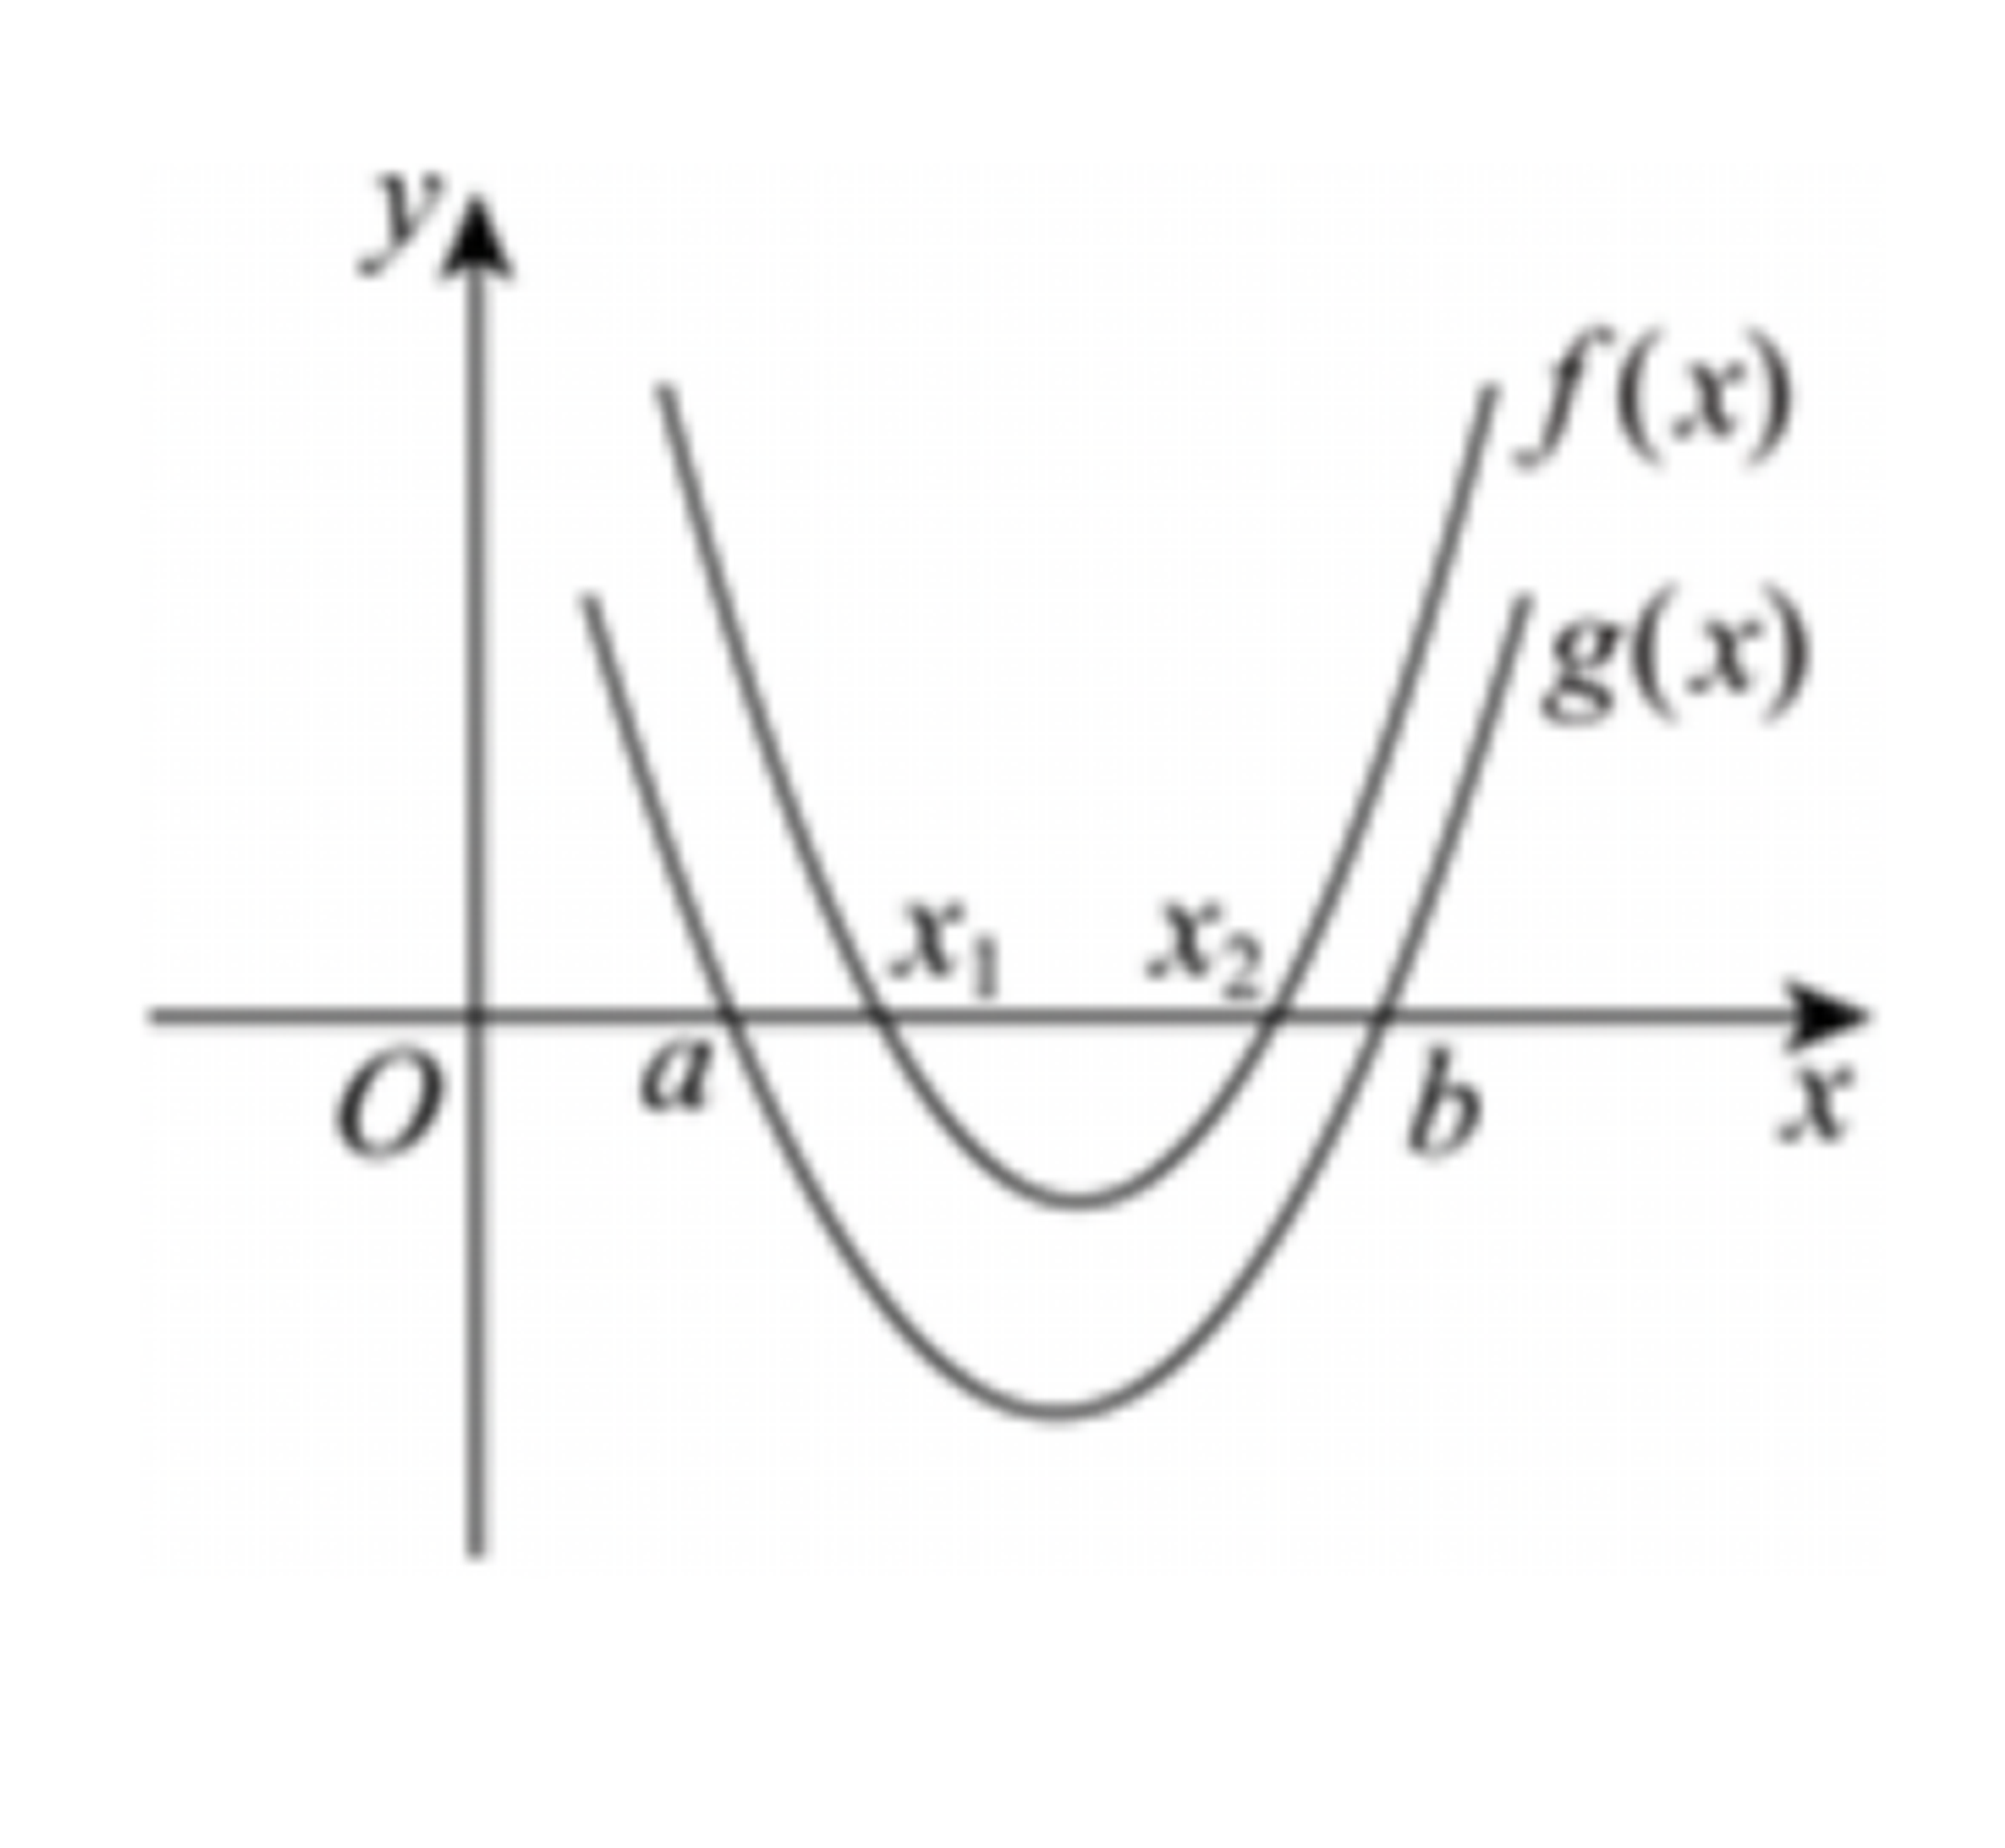
\includegraphics[width=0.30\textwidth]{figures/parabola_f_g_x1x2_h65.png}
\end{center}
\step{由图像得 $a<x_1<x_2<b$，故选 $B$.}
\solend
\fi

\end{enumerate}

\bigsec{三、解答题}

\begin{enumerate}
\setcounter{enumi}{16}

\item 已知 $a>0$，$b>0$，若 $a+b>4$，求证：$\dfrac a{b+2}$ 和 $\dfrac b{a+2}$ 中至少有一个大于 $\dfrac12$.

\ifanswer
\solbegin
\step{假设 $\dfrac a{b+2}\leqslant\dfrac12$，$\dfrac b{a+2}\leqslant\dfrac12$，}
\step{$a>0$，$b>0$，则 $a+2>0$，$b+2>0$，故 $2a\leqslant b+2$，$2b\leqslant a+2$，}
\step{两式相加得 $a+b\leqslant4$，与 $a+b>4$ 矛盾，故 $\dfrac a{b+2}$ 和 $\dfrac b{a+2}$ 中至少有一个大于 $\dfrac12$.}
\solend
\fi

\ansspace[6]

\item 已知集合 $A=\{x\mid-4<x<5\}$，$B=\{x\mid x\leqslant a-6\text{ 或 }x\geqslant a+2\}$.

\begin{enumerate}[label=(\arabic*)]

\item 若 $A\cup B=\R$，求实数 $a$ 的取值范围；

\item 若“$x\in A$”是“$x\in B$”的充分不必要条件，求实数 $a$ 的取值范围.

\end{enumerate}

\ifanswer
\solbegin
\stepm{(1)}{集合 $A=\{x\mid-4<x<5\}$，$B=\{x\mid x\leqslant a-6\text{ 或 }x\geqslant a+2\}$.}
\step{由 $A\cup B=\R$ 得 $\begin{cases}a-6\geqslant-4\\ a+2\leqslant5\end{cases}$，解得 $2\leqslant a\leqslant3$，$a$ 的取值范围为 $[2,3]$；}
\stepm{(2)}{若“$x\in A$”是“$x\in B$”的充分不必要条件，则 $A\subset B$，}
\step{则 $5\leqslant a-6$ 或 $-4\geqslant a+2$，解得 $a\leqslant-6$ 或 $a\geqslant11$.}
\solend
\fi

\ansspace[8]

% 注：原卷题干把命题 $P$ 印作“$\exists3\notin A$”（多一个存在量词），而【解析】两处均作
%     “$3\notin A$”；照录未改，见文件头“原卷笔误/存疑”③。
\item 已知集合 $A=\left\{x\mid\dfrac{x-1}{x-m}<0\right\}$，集合 $B=\left\{x\mid\left|\dfrac{x-1}{x-3}\right|\geqslant1\right\}$，命题 $P$：“$\exists3\notin A$”，命题
$Q$：$A\cap B\neq\varnothing$.

\begin{enumerate}[label=(\arabic*)]

\item 若命题 $P$ 为真命题，求 $m$ 的取值范围；

\item 若命题 $P$ 和命题 $Q$ 至少有一个为假命题，求实数 $m$ 的取值范围.

\end{enumerate}

\ifanswer
\solbegin
\stepm{(1)}{$A=\left\{x\mid\dfrac{x-1}{x-m}<0\right\}=\{x\mid(x-1)(x-m)<0\}$，}
\step{若命题 $P$：“$3\notin A$”为真命题，则 $(3-1)(3-m)\geqslant0$，解得 $m\leqslant3$，}
\step{故实数 $m$ 的取值范围为 $(-\infty,3]$；}
\stepm{(2)}{$B=\left\{x\mid\left|\dfrac{x-1}{x-3}\right|\geqslant1\right\}$，由 $\left|\dfrac{x-1}{x-3}\right|\geqslant1$，得 $\begin{cases}|x-1|\geqslant|x-3|\\ x\neq3\end{cases}$，}
\step{等价于 $\begin{cases}(x-1)^2\geqslant(x-3)^2\\ x\neq3\end{cases}$，解得 $x\geqslant2$ 且 $x\neq3$，所以 $B=[2,3)\cup(3,+\infty)$，}
\step{因为 $A=\{x\mid(x-1)(x-m)<0\}$，}
\step{当 $m=1$ 时，$A=\varnothing$，不满足 $A\cap B\neq\varnothing$，}
\step{当 $m<1$ 时，$A=(m,1)$，不满足 $A\cap B\neq\varnothing$，}
\step{当 $m>1$ 时，$A=(1,m)$，要使 $A\cap B\neq\varnothing$，则 $m>2$，}
\step{则若命题 $Q$：“$A\cap B\neq\varnothing$”为真命题时，实数 $m$ 的取值范围为 $(2,+\infty)$，}
\step{当命题 $P$ 与命题 $Q$ 都是真命题时，则 $\begin{cases}m\leqslant3\\ m>2\end{cases}$，解得 $2<m\leqslant3$，}
\step{则命题 $P$ 和命题 $Q$ 至少有一个为假命题时，得 $m\leqslant2$ 或 $m>3$，}
\step{故实数 $m$ 的取值范围为 $(-\infty,2]\cup(3,+\infty)$.}
\solend
\fi

\ansspace[8]

\item 已知函数 $y=ax^2-(a+2)x+2$，$a\in\R$.

\begin{enumerate}[label=(\arabic*)]

\item $y<3-2x$ 恒成立，求实数 $a$ 的取值范围；

% 注：原卷末句作“求实数 $a$ 的取值”（疑脱“范围”二字），照录未改，
%     见文件头“原卷笔误/存疑”⑤。
\item 若存在 $m>0$ 使关于 $x$ 的方程 $ax^2-(a+2)|x|+2=m+\dfrac1m+1$ 有四个不同的实根，
求实数 $a$ 的取值.

\end{enumerate}

\ifanswer
\solbegin
\stepm{(1)}{由题意得 $ax^2-(a+2)x+2<3-2x$ 恒成立，}
\step{即 $ax^2-ax-1<0$ 恒成立，}
\step{当 $a=0$ 时，$-1<0$ 恒成立，符合题意，}
\step{当 $a\neq0$ 时，则 $\begin{cases}a<0\\ \triangle=a^2+4a<0\end{cases}$，得 $\begin{cases}a<0\\ -4<a<0\end{cases}$，得 $-4<a<0$，}
\step{综上，$a$ 的取值范围为 $(-4,0]$.}
\stepm{(2)}{当 $m>0$ 时，令 $t=m+\dfrac1m+1\geqslant2\sqrt{m\times\dfrac1m}+1=3$，}
\step{当且仅当 $m=1$ 时取等号，}
% 注：题干只给“函数 $y=ax^2-(a+2)x+2$”，全卷未设 $f$，此处 $f(|x|)$ 无定义；
%     照录未改，见文件头“原卷笔误/存疑”④。
\step{则关于 $x$ 的方程 $f(|x|)=t$ 可化为 $a|x|^2-(a+2)|x|+2-t=0$，}
\step{关于 $x$ 的方程为 $a|x|^2-(a+2)|x|+2-t=0$ 有四个不等的实数根，}
\step{即 $ax^2-(a+2)x+2-t=0$，有两个不同的实数正根，}
\step{则 $\begin{cases}\triangle=(a+2)^2-4a(2-t)>0\\ \dfrac{a+2}a>0\\ \dfrac{2-t}a>0\end{cases}$，解得 $a<-2$，}
\step{由（1）得存在 $t\in[3,+\infty)$ 使得不等式 $4at+(a+2)^2-8a>0$ 成立，}
\step{故 $4a\times3+(a+2)^2-8a>0$，即 $a^2+8a+4>0$，}
\step{解得 $a<-4-2\sqrt3$ 或 $a>-4+2\sqrt3$，}
\step{综上，$a<-4-2\sqrt3$，所以 $a$ 的取值范围为 $(-\infty,-4-2\sqrt3)$.}
\solend
\fi

\ansspace[8]

\item 若集合 $A=B_1\cup B_2\cup\cdots\cup B_n$，其中 $B_1$、$B_2$、$\cdots$、$B_n$ 为非空集合，
$B_i\cap B_j=\varnothing$($1\leqslant i<j\leqslant n$)，则称集合 $\{B_1,B_2,\cdots,B_n\}$ 为集合 $A$ 的一个 $n$ 划分.

\begin{enumerate}[label=(\arabic*)]

\item 写出集合 $A=\{1,2,3\}$ 的所有不同的 2 划分；

\item 设 $\{B_1,B_2\}$ 为有理数集 $\Q$ 的一个 2 划分，且满足对任意 $x\in B_1$，任意 $y\in B_2$，都有
$x<y$，判断命题“$B_1$ 中的元素存在最大值，$B_2$ 中的元素存在最小值.”的真假，并说明
理由.

\item 设集合 $A=\{1,2,3,\cdots,16\}$，对于集合 $A$ 的任意一个 3 划分 $\{B_1,B_2,B_3\}$，判断是否存
在 $i\in\{1,2,3\}$，存在 $a$、$b\in B_i$，使得 $b-a\in B_i$ 成立，并说明理由.

\end{enumerate}

\ifanswer
\solbegin
% 注：原卷三个“2 划分”本有外层花括号（$\{\{1,2\},\{3\}\}$ 等），首轮误脱；
%     第二轮复核照原卷补回（原卷原样 / 本稿原错处：原脱外层花括号）。
\stepm{(1)}{集合 $A=\{1,2,3\}$ 的所有不同的 2 划分为 $\{\{1,2\},\{3\}\}$、$\{\{1,3\},\{2\}\}$、}
\step{$\{\{2,3\},\{1\}\}$.}
\stepm{(2)}{该命题为假命题，理由如下：}
\step{假设命题为真，则不妨设 $B_1$ 中元素的最大值为 $s$，$B_2$ 中元素的最小值为 $t$，}
\step{由题意得 $s<t$，所以 $s<\dfrac{s+t}2<t$，}
\step{因为 $s$ 为 $B_1$ 中元素的最大值，所以 $\dfrac{s+t}2\notin B_1$，}
\step{因为 $t$ 为 $B_2$ 中元素的最小值，所以 $\dfrac{s+t}2\notin B_2$，}
\step{因为 $B_1\cup B_2=\Q$，所以 $\dfrac{s+t}2\notin\Q$，}
\step{这与 $\dfrac{s+t}2\in\Q$ 矛盾，所以假设不成立，即命题不可能成立；}
\stepm{(3)}{由于集合 $A$ 中有 16 个元素，}
\step{所以 $B_1$、$B_2$、$B_3$ 中至少有一个集合至少包含 6 个元素，}
\step{不妨设 $B_1$ 中至少包含 6 个元素，}
\step{设 $b_1$、$b_2$、$b_3$、$b_4$、$b_5$、$b_6\in B_1$，且 $b_1<b_2<b_3<b_4<b_5<b_6$，}
\step{假设对任意 $i\in\{1,2,3\}$，对任意 $a$、$b\in B_i$，都有 $b-a\notin B_i$，}
\step{那么 $b_6-b_1$、$b_6-b_2$、$b_6-b_3$、$b_6-b_4$、$b_6-b_5\notin B_1$，}
\step{又因为 $b_6-b_1$、$b_6-b_2$、$b_6-b_3$、$b_6-b_4$、$b_6-b_5\in A$，}
\step{所以 $b_6-b_1$、$b_6-b_2$、$b_6-b_3$、$b_6-b_4$、$b_6-b_5\in B_2\cup B_3$，}
\step{则 $B_2$、$B_3$ 中必有一个集合}
\step{至少包含 $b_6-b_1$、$b_6-b_2$、$b_6-b_3$、$b_6-b_4$、$b_6-b_5$ 中的 3 个元素，}
\step{不妨设这 3 个元素为 $a_1$、$a_2$、$a_3\in B_2$，$a_1<a_2<a_3$，}
\step{由假设得 $a_3-a_1$、$a_3-a_2$、$a_2-a_1\notin B_2$，}
\step{对任意 $i$、$j$($1\leqslant j<i\leqslant3$)，存在 $m$、$n$($1\leqslant m<n\leqslant5$)，}
\step{都有 $a_i-a_j=b_6-b_m-b_6+b_n=b_n-b_m\notin B_1$，}
\step{又因为 $a_3-a_1$、$a_3-a_2$、$a_2-a_1\in B_3$，而 $a_3-a_1-(a_3-a_2)=a_2-a_1$，}
\step{与假设矛盾，所以假设不成立，}
\step{即存在 $i\in\{1,2,3\}$，存在 $a$、$b\in B_i$，使得 $b-a\in B_i$.}
\solend
\fi

\ansspace*[10]

\end{enumerate}

\end{document}
"
%
% 原始材料：微信公众号“魔都数学加油站”文章，作者破晓，连载“27学年高一65”；
% 原文标题“27学年高一65——2026-2027年上海市大同中学高一上10月月考”；
% 原文链接：https://mp.weixin.qq.com/s/h9ctuk-ByE1Vfg2Rx2C6bw。
% 页面标注发布时间 2026-10-17 21:58（上海）。
% 本次转录只据 `原图/高一65_大同中学_10月月考/` 的 11 张 PNG 逐页读图。
% 正文为 11 张 PNG 页（`01..11.png`）：
% 第 06、11 页 2560×3620，第 01、02、03、04、05、07、08、09、10 页 4762×6735
% （**同一篇各页分辨率不同**），均按页序读取。11 页全为试卷正文页（卷首标题在第 1 页页顶，
% 卷末解答题第 21 题解析止于第 11 页），无封面页、目录页、二维码或宣传页。
% 粉色斜排“魔都数学加油站”为卷面水印，与公众号页脚一并未录入。
%
% 卷首标题：照卷面印作“2026--2027 年大同中学高一上 10 月月考”，年份区间按全稿惯例排 en dash。
% 原卷只有一行标题、无副标题。
%
% 篇幅与题号：原卷自第 3 题起编号（第 1、2 题不在本卷内）。填空题 3—12（10 题）、
% 选择题 13—16（4 题）、解答题 17—21（5 题），共 19 题。本稿沿用原节与原题号，
% 只改排为全稿统一的大节样式（原卷小节标题为“一、填空题”“二、选择题”“三、解答题”）。
%
% 讲评版：原卷每题下直接印【答案】或【解析】。**只印【答案】的 4 题**（第 3、4、7、10 题），
% 本稿只给 \ans{}；其余 15 题都印【解析】（按全稿口径这类题不另提 \ans{}——第 12、13、14、
% 15、16 题的结论写在解析末句（“故选 B”“综上，n 的最大值为 14”等），亦照录在解析内）。
% 全卷无“答案印在题干括号内”的题（第 13—16 题的选择题括号内均空白）。
%
% 副标题：原卷未印副标题。本稿按“知识模块”口径标作“集合与常用逻辑用语、不等式”：
% 19 题中集合与常用逻辑用语 10 题（第 3、4、6、8、12、14、15、18、19、21 题），
% 不等式 9 题（含等式恒等、不等式性质、二次不等式、恒成立、基本不等式、不等式的证明：
% 第 5、7、9、10、11、13、16、17、20 题），两类均超过三分之一，故并标。口径同 高一63。
%
% 与原卷的排版差异：
%   ① 原卷每题下直接印【答案】/【解析】，本稿按全稿惯例将答案与解析置于答案版，试卷版保持干净；
%   ② 原卷未印副标题，本稿按“知识模块”口径补出；
%   ③ 原卷填空横线约四个字宽，本稿按全稿惯例统一排 \blankline[4.4em]；
%   ④ 原卷数集记号全为斜体：实数集作 $R$（第 6 题两处、第 8 题两处、第 15 题解析、第 18 题、
%      第 20 题题干），自然数集作 $N$（第 12 题题干“$n\in N,n\geqslant1$”），有理数集作 $Q$
%      （第 21 题 (2) 题干与解析共 4 处），本稿按全稿惯例统一改用 $\R$、$\N$、$\Q$
%      （同 高一63 排版差异④：记号归一）；空集记号原卷作 $\varnothing$，照录；
%   ⑤ 原卷用描述法时竖线排细竖“$|$”（如 $\{x|0<x<3\}$、$\{x|(x-1)(x-m)<0\}$），
%      本稿按全稿惯例排 \mid；
%   ⑥ 原卷判别式印作“$\triangle$”（第 8、14 题解析各 1 处、第 20 题解析 2 处，共 4 处），
%      本稿照录用 \triangle（同 高一39 成例），未改作 \Delta；
%   ⑦ 第 18—21 题的子问原卷各自另起一行、以“（1）”“（2）”标号，本稿按全稿惯例用
%      enumerate 的 (1)(2)(3)；解析中的子问标号一律用 \stepm{(1)}{…}；
%      第 18—21 题解析（原文以“（1）”“（2）”“（3）”冠于解析首句）同此；
%   ⑧ 选择题的作答括号原卷排半角“(　　)”（第 13—16 题括号内均空白），
%      本稿按全稿惯例排 \mbox{（\quad）}；选项字母后的句点照原卷排“A.”“B.”；
%   ⑨ 每道解答题原卷未留作答空白，本稿按全稿惯例加 \ansspace（末题用 \ansspace*）；
%   ⑩ 原卷在数学式内多处用半角逗号（如 $\{x|0<x<3\},B=\{x|x>2\}$、$m\in I_{14},k\in I_{14}$），
%      均照录未强改；句末句点按全稿惯例排西文句点。
%
% 原卷笔误/存疑（均照录未改，正文对应处另有 % 注）：
%   ① 第 13 题题干“下列不等式中一定成立是（　　）”脱一个“的”（当作“一定成立的是”），
%      8 倍放大确认非水印遮挡，本稿照录；
%   ② 第 15 题【解析】末段把题干条件“$x\geqslant10$”写成“$x\geqslant1$”
%      （“所以 $x+2+\frac{16}{x+2}(x\geqslant1)$ 的最小值不为 8”），与同段前面“令 $t=x+2$，
%      则 $t\geqslant12$”不合，本稿照录；
%   ③ 第 19 题题干把命题 $P$ 印作“$\exists3\notin A$”（多一个存在量词），而【解析】两处
%      均作“$3\notin A$”，前后记号不一，本稿照录；
%   ④ 第 20 题【解析】(2) 出现 $f(|x|)$，但题干只给“函数 $y=ax^2-(a+2)x+2$”、全卷未设 $f$，
%      本稿照录；
%   ⑤ 第 20 题 (2) 题干末句作“求实数 $a$ 的取值”（疑脱“范围”二字），本稿照录；
%   ⑥ 第 12 题【解析】第 18 步“它与 $P_n$ 中的任何其他数之和都不是整数”，该段所论为 $P_{14}$
%      （前后均作 $P_{14}$），此处 $P_n$ 疑当作 $P_{14}$，本稿照录。
%
% 第二轮复核（2026-10-18）订正「本稿抄错原卷」一处：
%   第 21 题 (1)【解析】原卷本作“$\{\{1,2\},\{3\}\}$、$\{\{1,3\},\{2\}\}$、$\{\{2,3\},\{1\}\}$”，
%   有外层花括号；首轮误脱外层花括号，并曾在文件头误记为“原卷未加外层花括号”（原第 ⑦ 条，
%   已撤销）。本次照原卷补回，正文对应处另有 % 注。
%
% 插图：第 16 题【解析】内有 1 幅图（两条开口向上的抛物线 $f(x)$、$g(x)$ 与 $x$ 轴交点
% 标 $a$、$x_1$、$x_2$、$b$，纵轴标 $y$、原点 $O$），解析第三行“画出函数 $g(x)$ 与函数 $f(x)$
% 的图像，如图所示”即指此图；取原卷截图（06.png，2560×3620）右半幅，4× LANCZOS 放大，
% 存 figures/parabola_f_g_x1x2_h65.png。该图在【解析】内，仅答案版出。
%
\documentclass[a4paper,11pt]{article}
\usepackage{common}

\begin{document}

\examtitlest[3]{2026--2027 年大同中学高一上 10 月月考}{集合与常用逻辑用语、不等式}

\bigsec{一、填空题}

\begin{enumerate}
\setcounter{enumi}{2}

\item 已知集合 $A=\{x\mid0<x<3\}$,$B=\{x\mid x>2\}$，则集合 $A\cup B=$\blankline[4.4em].

\ifanswer
\ans{$(0,+\infty)$}
\fi

\item “$x>1$ 或 $y>1$”的否定形式是\blankline[4.4em].

\ifanswer
\ans{$x\leqslant1$ 且 $y\leqslant1$}
\fi

\item 已知等式 $2x^2+3x+4=a(2x+1)(x+1)+b$ 恒成立，则常数 $a-b=$\blankline[4.4em].

\ifanswer
\solbegin
\step{因为等式 $2x^2+3x+4=a(2x+1)(x+1)+b$ 恒成立，}
\step{所以 $a(2x+1)(x+1)+b=2ax^2+3ax+a+b=2x^2+3x+4$，}
\step{所以 $\begin{cases}2a=2\\ 3a=3\\ a+b=4\end{cases}$，解得 $\begin{cases}a=1\\ b=3\end{cases}$，所以 $a-b=-2$.}
\solend
\fi

\item 全集为 $U=\R$，$A=\{x\mid|x|\geqslant2\}$，$B=\{y\mid y=x^2+1,x\in\R\}$，则 $A\cup\bar B=$\blankline[4.4em].

\ifanswer
\solbegin
\step{由题意得集合 $A=\{x\mid x\geqslant2\text{ 或 }x\leqslant-2\}$，}
\step{因为 $x^2+1\geqslant1$，所以集合 $B=\{x\mid x\geqslant1\}$，所以 $\bar B=\{x\mid x<1\}$，}
\step{则 $A\cup\bar B=\{x\mid x\geqslant2\text{ 或 }x<1\}$.}
\solend
\fi

\item 已知 $|x+3|+|x-5|=8$，则实数 $x$ 的取值范围为\blankline[4.4em].

\ifanswer
\ans{$[-3,5]$}
\fi

\item 已知集合 $A=\{x\in\R\mid ax^2+2x+1=0,a\in\R\}$ 只有一个元素，则 $a$ 的值为\blankline[4.4em].

\ifanswer
\solbegin
\step{当 $a=0$ 时，$A=\left\{-\dfrac12\right\}$；}
\step{当 $a\neq0$ 时，若集合 $A$ 只有一个元素，由 $\triangle=4-4a=0$ 得 $a=1$.}
\step{综上，当 $a=0$ 或 $a=1$ 时，集合 $A$ 只有一个元素.}
\solend
\fi

\item 已知不等式 $-x^2+bx+c>0$ 的解集为 $(3,4)$，则不等式 $cx^2+bx-1<0$ 的解集为\blankline[4.4em].

\ifanswer
\solbegin
\step{由题意得 3，4 是方程 $-x^2+bx+c=0$ 的两个实数根，}
\step{所以 $\begin{cases}3+4=b\\ 3\times4=-c\end{cases}$，得 $b=7$，$c=-12$，}
\step{则不等式 $cx^2+bx-1<0$，即为 $-12x^2+7x-1<0$，即 $12x^2-7x+1>0$，}
\step{化简得 $(3x-1)(4x-1)>0$，解得 $x<\dfrac14$ 或 $x>\dfrac13$，}
\step{即不等式 $cx^2+bx-1<0$ 的解集为 $\left(-\infty,\dfrac14\right)\cup\left(\dfrac13,+\infty\right)$.}
\solend
\fi

\item 对于区间 $(m,n)$，我们将 $n-m$ 的值称为该区间的长度. 若关于 $x$ 的不等式
$x^2+ax+a<0$ 有解，且解集的区间长度不超过 $2\sqrt3$，则实数 $a$ 的取值范围是\blankline[4.4em].

\ifanswer
\ans{$[-2,0)\cup(4,6]$}
\fi

\item 当 $x>0$ 时，关于 $x$ 的不等式 $(ax-1)(x^2+bx-4)\geqslant0$ 恒成立，则 $b+\dfrac2a$ 的最小值
为\blankline[4.4em].

\ifanswer
\solbegin
\step{由题意 $a\neq0$；}
\step{若 $a<0$，则 $x>0$ 时 $ax-1<0$ 恒成立，需 $x^2+bx-4\leqslant0$ 对一切 $x>0$ 成立，}
\step{而 $y=x^2+bx-4$ 的图象开口向上，当 $x$ 充分大时必为正值，矛盾，故 $a>0$.}
\step{当 $a>0$ 时，$ax-1=a\left(x-\dfrac1a\right)$，故原条件化为 $\left(x-\dfrac1a\right)(x^2+bx-4)\geqslant0$：}
\step{若 $0<x<\dfrac1a$，则 $x-\dfrac1a<0$，需 $x^2+bx-4\leqslant0$；}
\step{若 $x>\dfrac1a$，则 $x-\dfrac1a>0$，需 $x^2+bx-4\geqslant0$；}
\step{由 $y=x^2+bx-4$ 的连续性知 $x=\dfrac1a$ 是它的零点，}
\step{即 $\dfrac1{a^2}+\dfrac ba-4=0$，得 $b=4a-\dfrac1a$；}
\step{此时 $x^2+bx-4=x^2+\left(4a-\dfrac1a\right)x-4=(x+4a)\left(x-\dfrac1a\right)$，}
\step{由 $a>0$、$x>0$ 得 $x+4a>0$，}
\step{其符号与 $x-\dfrac1a$ 一致，故能与 $ax-1$ 同号，原不等式确在 $x>0$ 上恒成立.}
\step{于是 $b+\dfrac2a=4a-\dfrac1a+\dfrac2a=4a+\dfrac1a\geqslant2\sqrt{4a\cdot\dfrac1a}=4$，}
\step{当且仅当 $a=\dfrac12$ 时取等号，故最小值为 4.}
\solend
\fi

\item 设集合 $I_n=\{1,2,\cdots,n\}$，$n\in\N$，$n\geqslant1$，集合 $P_n=\left\{\dfrac m{\sqrt k}\mid m\in I_n,k\in I_n\right\}$，若 $P_n$ 的子集 $A$
中任意两个元素之和不是整数的平方，则称 $A$ 为“人文集”. 那么使 $P_n$ 能分成两个交集为空
集的“人文集”的并集，且这两个人文集的并集恰为 $P_n$ 时，$n$ 的最大值是\blankline[4.4em].

\ifanswer
\solbegin
\step{先证当 $n\geqslant15$ 时，$P_n$ 不能分成两个不相交的人文集的并集.}
\step{假设当 $n\geqslant15$ 时，$P_n$ 可以分成两个不相交的人文集的并集，}
\step{设 $A$ 和 $B$ 为两个不相交的人文集，使 $A\cup B=P_n\supseteq I_n$.}
\step{不妨设 $1\in A$，则由于 $1+3=2^2$，所以 $3\notin A$，即 $3\in B$.}
\step{同理可得，$6\in A$，$10\in B$. 又推出 $15\in A$，}
\step{但 $1+15=4^2$，这与 $A$ 为人文集相矛盾.}
\step{再证 $P_{14}$ 满足要求. 当 $k=1$ 时，$P_{14}=\left\{\dfrac m{\sqrt k}\mid m\in I_{14},k\in I_{14}\right\}$，}
\step{可以分成 2 个人文集的并集.}
\step{事实上，只要取 $A_1=\{1,2,4,6,9,11,13\}$，$B_1=\{3,5,7,8,10,12,14\}$，}
\step{则 $A_1$ 和 $B_1$ 都是人文集，且 $A_1\cup B_1=P_{14}$.}
\step{当 $k=4$ 时，集合 $\left\{\dfrac m{\sqrt k}\mid m\in I_{14}\right\}$ 中，除整数外，}
\step{剩下的数组成集合 $\left\{\dfrac12,\dfrac32,\dfrac52,\cdots,\dfrac{13}2\right\}$，}
\step{可以分为下列 2 个人文集的并：$A_2=\left\{\dfrac12,\dfrac52,\dfrac92,\dfrac{11}2\right\}$，$B_2=\left\{\dfrac32,\dfrac72,\dfrac{13}2\right\}$.}
\step{当 $k=9$ 时，集合 $\left\{\dfrac m{\sqrt k}\mid m\in I_{14}\right\}$ 中，除整数外，}
\step{剩下的数组成集合 $\left\{\dfrac13,\dfrac23,\dfrac43,\dfrac53,\cdots,\dfrac{13}3,\dfrac{14}3\right\}$，}
\step{可以分为下列 2 个人文集的并：$A_3=\left\{\dfrac13,\dfrac43,\dfrac53,\dfrac{10}3,\dfrac{13}3\right\}$，$B_3=\left\{\dfrac23,\dfrac73,\dfrac83,\dfrac{11}3,\dfrac{14}3\right\}$.}
\step{最后，集合 $C=\left\{\dfrac m{\sqrt k}\mid m\in I_{14},k\in I_{14},k\neq1,4,9\right\}$ 中的数的分母都是无理数，}
% 注：本行原卷作“$P_n$”，而该段所论为 $P_{14}$（前后均作 $P_{14}$），疑当作 $P_{14}$；
%     照录未改，见文件头“原卷笔误/存疑”⑥。
\step{它与 $P_n$ 中的任何其他数之和都不是整数，}
\step{因此，令 $A=A_1\cup A_2\cup A_3\cup C$，$B=B_1\cup B_2\cup B_3$，}
\step{则 $A$ 和 $B$ 是不相交的人文集，且 $A\cup B=P_{14}$.}
\step{综上，$n$ 的最大值为 14.}
\solend
\fi

\end{enumerate}

\bigsec{二、选择题}

\begin{enumerate}
\setcounter{enumi}{12}

% 注：原卷题干“下列不等式中一定成立是”脱一个“的”（当作“一定成立的是”），
%     照录未改，见文件头“原卷笔误/存疑”①。
\item 已知 $a>b$，下列不等式中一定成立是\mbox{（\quad）}

\keepwithprev
A. $a^2>b^2$\qquad B. $ac^2>bc^2$\qquad C. $\dfrac1a<\dfrac1b$\qquad D. $a+3>b-4$

\ifanswer
\solbegin
\step{对于 $A$，当 $a=-2$，$b=-4$ 时，不等式不成立，故 $A$ 错误；}
\step{对于 $B$，当 $c=0$ 时，不等式不成立，故 $B$ 错误；}
\step{对于 $C$，当 $a=2$，$b=-4$ 时，不等式不成立，故 $C$ 错误；}
\step{对于 $D$，因为 $a>b$，$3>-4$，必有 $a+3>b-4$ 成立，故 $D$ 正确.}
\step{故选 $D$.}
\solend
\fi

\item 已知 $a$ 为实数，那么“$|a|\leqslant2$”是“方程 $x^2+ax+1=0$ 没有实数解”的\mbox{（\quad）}

\keepwithprev
A. 充分而不必要条件\qquad B. 必要而不充分条件

C. 充要条件\qquad D. 既不充分也不必要条件

\ifanswer
\solbegin
\step{由方程 $x^2+ax+1=0$ 没有实数解，得 $\triangle=a^2-4<0$，则 $|a|<2$，}
\step{由 $|a|<2$ 得 $|a|\leqslant2$，反之不成立，}
\step{所以“$|a|\leqslant2$”是“方程 $x^2+ax+1=0$ 没有实数解”的必要而不充分条件.}
\step{故选 $B$.}
\solend
\fi

\item 下列命题为真命题的是\mbox{（\quad）}

\keepwithprev
A. $a>b>0$，当 $m>0$ 时，$\dfrac{a+m}{b+m}>\dfrac ab$

B. 集合 $A=\{x\mid y=x^2+1\}$ 与集合 $B=\{y\mid y=x^2+1\}$ 是相同的集合

C. 若 $b<a<0$，$m<0$，则 $\dfrac ma>\dfrac mb$

D. $x+2+\dfrac{16}{x+2}(x\geqslant10)$ 最小值为 8

\ifanswer
\solbegin
\step{对于 $A$，$\dfrac{a+m}{b+m}-\dfrac ab=\dfrac{b(a+m)-a(b+m)}{b(b+m)}=\dfrac{m(b-a)}{b(b+m)}$，}
\step{因为 $a>b>0$，$m>0$，所以 $b(b+m)>0$，$m(b-a)<0$，}
\step{所以 $\dfrac{a+m}{b+m}-\dfrac ab=\dfrac{m(b-a)}{b(b+m)}<0$，}
\step{即 $a>b>0$，当 $m>0$ 时，$\dfrac{a+m}{b+m}<\dfrac ab$，故 $A$ 错误；}
\step{对于 $B$，集合 $A=\{x\mid y=x^2+1\}=\R$，集合 $B=\{y\mid y=x^2+1\}=\{y\mid y\geqslant1\}$，}
\step{所以 $A\neq B$，故 $B$ 错误；}
\step{对于 $C$，$\dfrac ma-\dfrac mb=\dfrac{m(b-a)}{ab}$，}
\step{因为 $b<a<0$，$m<0$，所以 $ab>0$，$m(b-a)>0$，}
\step{所以 $\dfrac ma-\dfrac mb=\dfrac{m(b-a)}{ab}>0$，即 $\dfrac ma>\dfrac mb$，故 $C$ 正确；}
\step{对于 $D$，令 $t=x+2$，则 $t\geqslant12$，表达式变为 $t+\dfrac{16}t$，}
\step{$t+\dfrac{16}t\geqslant2\sqrt{t\cdot\dfrac{16}t}=8$，当且仅当 $t=4$ 时取等号，即等号不成立，}
% 注：原卷本行把题干条件“$x\geqslant10$”写成“$x\geqslant1$”，与同段“$t\geqslant12$”不合；
%     照录未改，见文件头“原卷笔误/存疑”②。
\step{所以 $x+2+\dfrac{16}{x+2}(x\geqslant1)$ 的最小值不为 8，故 $D$ 错误.}
\step{故选 $C$.}
\solend
\fi

\item 已知实数 $a<b$，关于 $x$ 的不等式 $x^2-(a+b)x+ab+\dfrac12<0$ 的解集为 $(x_1,x_2)$，则实数 $a$、
$b$、$x_1$、$x_2$ 从小到大的排列是\mbox{（\quad）}

\keepwithprev
A. $x_1<a<b<x_2$\qquad B. $a<x_1<x_2<b$\qquad C. $a<x_1<b<x_2$\qquad D. $x_1<a<x_2<b$

\ifanswer
\solbegin
\step{不等式 $x^2-(a+b)x+ab+\dfrac12<0$ 可化为 $(x-a)(x-b)+\dfrac12<0$，}
\step{设 $g(x)=(x-a)(x-b)$，$f(x)=g(x)+\dfrac12$，}
\step{画出函数 $g(x)$ 与函数 $f(x)$ 的图像，如图所示，}
% 图在【解析】内（仅答案版出），取原卷截图（06.png，2560×3620）右半幅，4× LANCZOS 放大。
\begin{center}
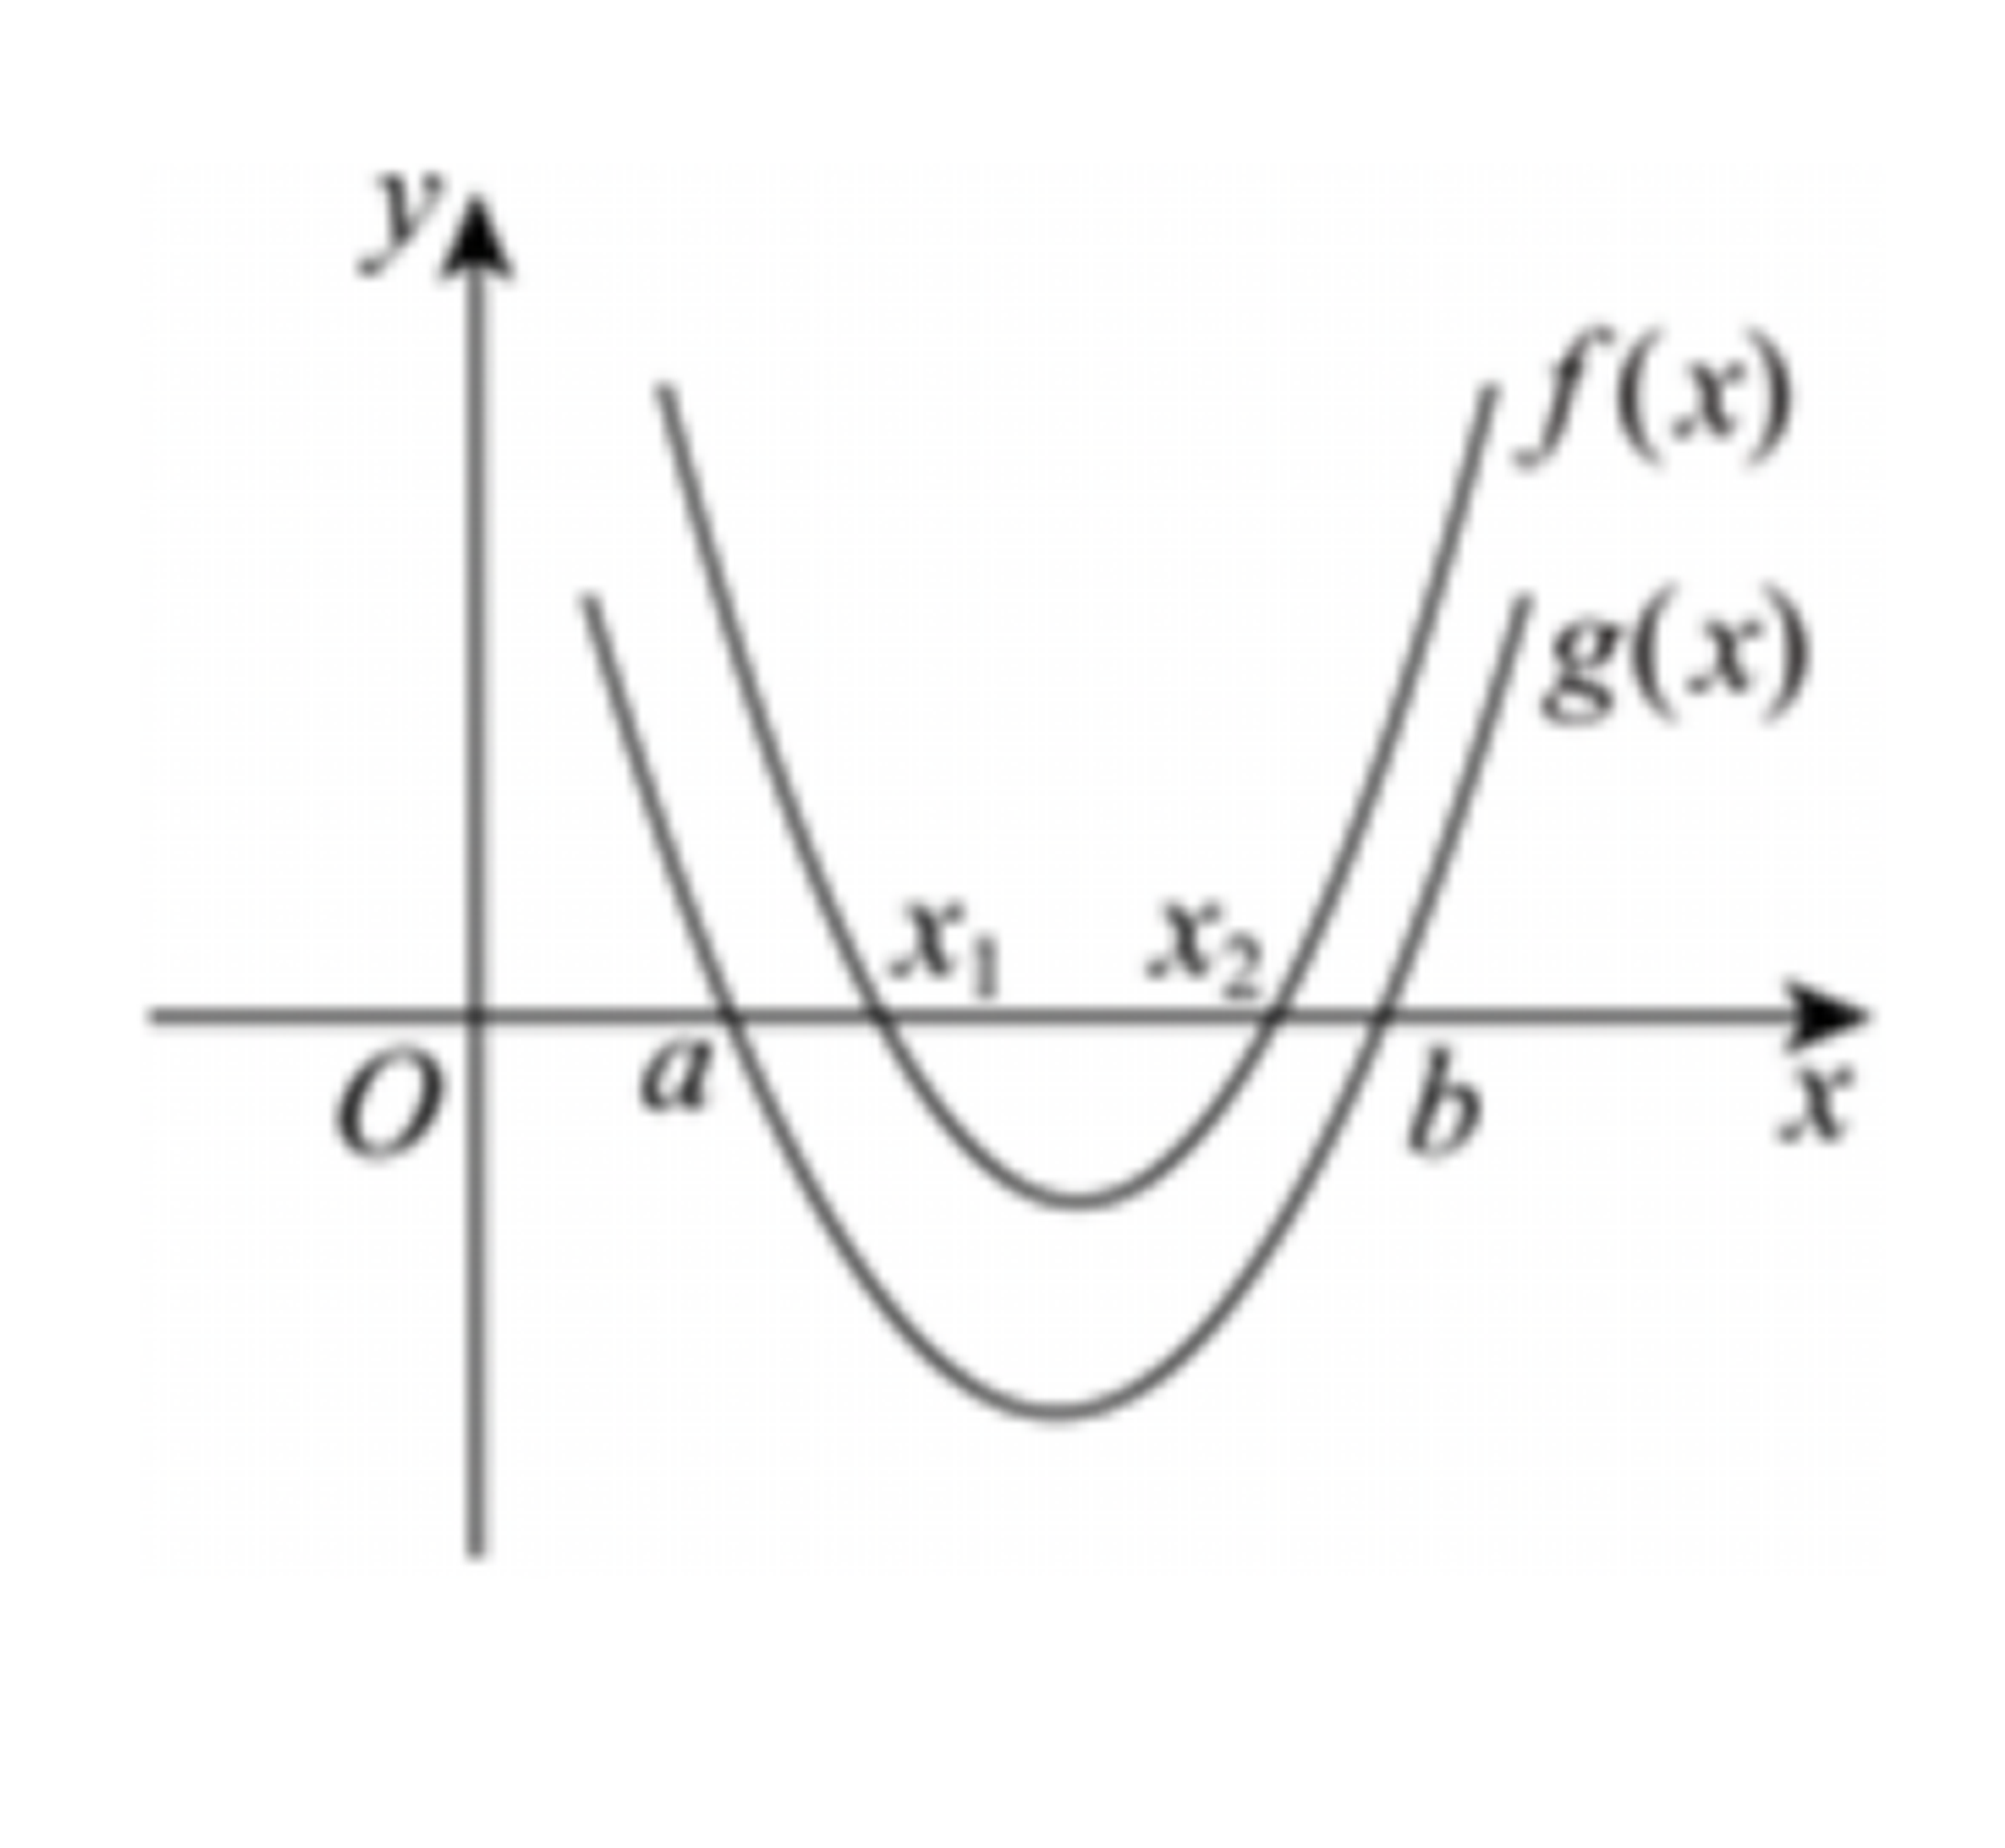
\includegraphics[width=0.30\textwidth]{figures/parabola_f_g_x1x2_h65.png}
\end{center}
\step{由图像得 $a<x_1<x_2<b$，故选 $B$.}
\solend
\fi

\end{enumerate}

\bigsec{三、解答题}

\begin{enumerate}
\setcounter{enumi}{16}

\item 已知 $a>0$，$b>0$，若 $a+b>4$，求证：$\dfrac a{b+2}$ 和 $\dfrac b{a+2}$ 中至少有一个大于 $\dfrac12$.

\ifanswer
\solbegin
\step{假设 $\dfrac a{b+2}\leqslant\dfrac12$，$\dfrac b{a+2}\leqslant\dfrac12$，}
\step{$a>0$，$b>0$，则 $a+2>0$，$b+2>0$，故 $2a\leqslant b+2$，$2b\leqslant a+2$，}
\step{两式相加得 $a+b\leqslant4$，与 $a+b>4$ 矛盾，故 $\dfrac a{b+2}$ 和 $\dfrac b{a+2}$ 中至少有一个大于 $\dfrac12$.}
\solend
\fi

\ansspace[6]

\item 已知集合 $A=\{x\mid-4<x<5\}$，$B=\{x\mid x\leqslant a-6\text{ 或 }x\geqslant a+2\}$.

\begin{enumerate}[label=(\arabic*)]

\item 若 $A\cup B=\R$，求实数 $a$ 的取值范围；

\item 若“$x\in A$”是“$x\in B$”的充分不必要条件，求实数 $a$ 的取值范围.

\end{enumerate}

\ifanswer
\solbegin
\stepm{(1)}{集合 $A=\{x\mid-4<x<5\}$，$B=\{x\mid x\leqslant a-6\text{ 或 }x\geqslant a+2\}$.}
\step{由 $A\cup B=\R$ 得 $\begin{cases}a-6\geqslant-4\\ a+2\leqslant5\end{cases}$，解得 $2\leqslant a\leqslant3$，$a$ 的取值范围为 $[2,3]$；}
\stepm{(2)}{若“$x\in A$”是“$x\in B$”的充分不必要条件，则 $A\subset B$，}
\step{则 $5\leqslant a-6$ 或 $-4\geqslant a+2$，解得 $a\leqslant-6$ 或 $a\geqslant11$.}
\solend
\fi

\ansspace[8]

% 注：原卷题干把命题 $P$ 印作“$\exists3\notin A$”（多一个存在量词），而【解析】两处均作
%     “$3\notin A$”；照录未改，见文件头“原卷笔误/存疑”③。
\item 已知集合 $A=\left\{x\mid\dfrac{x-1}{x-m}<0\right\}$，集合 $B=\left\{x\mid\left|\dfrac{x-1}{x-3}\right|\geqslant1\right\}$，命题 $P$：“$\exists3\notin A$”，命题
$Q$：$A\cap B\neq\varnothing$.

\begin{enumerate}[label=(\arabic*)]

\item 若命题 $P$ 为真命题，求 $m$ 的取值范围；

\item 若命题 $P$ 和命题 $Q$ 至少有一个为假命题，求实数 $m$ 的取值范围.

\end{enumerate}

\ifanswer
\solbegin
\stepm{(1)}{$A=\left\{x\mid\dfrac{x-1}{x-m}<0\right\}=\{x\mid(x-1)(x-m)<0\}$，}
\step{若命题 $P$：“$3\notin A$”为真命题，则 $(3-1)(3-m)\geqslant0$，解得 $m\leqslant3$，}
\step{故实数 $m$ 的取值范围为 $(-\infty,3]$；}
\stepm{(2)}{$B=\left\{x\mid\left|\dfrac{x-1}{x-3}\right|\geqslant1\right\}$，由 $\left|\dfrac{x-1}{x-3}\right|\geqslant1$，得 $\begin{cases}|x-1|\geqslant|x-3|\\ x\neq3\end{cases}$，}
\step{等价于 $\begin{cases}(x-1)^2\geqslant(x-3)^2\\ x\neq3\end{cases}$，解得 $x\geqslant2$ 且 $x\neq3$，所以 $B=[2,3)\cup(3,+\infty)$，}
\step{因为 $A=\{x\mid(x-1)(x-m)<0\}$，}
\step{当 $m=1$ 时，$A=\varnothing$，不满足 $A\cap B\neq\varnothing$，}
\step{当 $m<1$ 时，$A=(m,1)$，不满足 $A\cap B\neq\varnothing$，}
\step{当 $m>1$ 时，$A=(1,m)$，要使 $A\cap B\neq\varnothing$，则 $m>2$，}
\step{则若命题 $Q$：“$A\cap B\neq\varnothing$”为真命题时，实数 $m$ 的取值范围为 $(2,+\infty)$，}
\step{当命题 $P$ 与命题 $Q$ 都是真命题时，则 $\begin{cases}m\leqslant3\\ m>2\end{cases}$，解得 $2<m\leqslant3$，}
\step{则命题 $P$ 和命题 $Q$ 至少有一个为假命题时，得 $m\leqslant2$ 或 $m>3$，}
\step{故实数 $m$ 的取值范围为 $(-\infty,2]\cup(3,+\infty)$.}
\solend
\fi

\ansspace[8]

\item 已知函数 $y=ax^2-(a+2)x+2$，$a\in\R$.

\begin{enumerate}[label=(\arabic*)]

\item $y<3-2x$ 恒成立，求实数 $a$ 的取值范围；

% 注：原卷末句作“求实数 $a$ 的取值”（疑脱“范围”二字），照录未改，
%     见文件头“原卷笔误/存疑”⑤。
\item 若存在 $m>0$ 使关于 $x$ 的方程 $ax^2-(a+2)|x|+2=m+\dfrac1m+1$ 有四个不同的实根，
求实数 $a$ 的取值.

\end{enumerate}

\ifanswer
\solbegin
\stepm{(1)}{由题意得 $ax^2-(a+2)x+2<3-2x$ 恒成立，}
\step{即 $ax^2-ax-1<0$ 恒成立，}
\step{当 $a=0$ 时，$-1<0$ 恒成立，符合题意，}
\step{当 $a\neq0$ 时，则 $\begin{cases}a<0\\ \triangle=a^2+4a<0\end{cases}$，得 $\begin{cases}a<0\\ -4<a<0\end{cases}$，得 $-4<a<0$，}
\step{综上，$a$ 的取值范围为 $(-4,0]$.}
\stepm{(2)}{当 $m>0$ 时，令 $t=m+\dfrac1m+1\geqslant2\sqrt{m\times\dfrac1m}+1=3$，}
\step{当且仅当 $m=1$ 时取等号，}
% 注：题干只给“函数 $y=ax^2-(a+2)x+2$”，全卷未设 $f$，此处 $f(|x|)$ 无定义；
%     照录未改，见文件头“原卷笔误/存疑”④。
\step{则关于 $x$ 的方程 $f(|x|)=t$ 可化为 $a|x|^2-(a+2)|x|+2-t=0$，}
\step{关于 $x$ 的方程为 $a|x|^2-(a+2)|x|+2-t=0$ 有四个不等的实数根，}
\step{即 $ax^2-(a+2)x+2-t=0$，有两个不同的实数正根，}
\step{则 $\begin{cases}\triangle=(a+2)^2-4a(2-t)>0\\ \dfrac{a+2}a>0\\ \dfrac{2-t}a>0\end{cases}$，解得 $a<-2$，}
\step{由（1）得存在 $t\in[3,+\infty)$ 使得不等式 $4at+(a+2)^2-8a>0$ 成立，}
\step{故 $4a\times3+(a+2)^2-8a>0$，即 $a^2+8a+4>0$，}
\step{解得 $a<-4-2\sqrt3$ 或 $a>-4+2\sqrt3$，}
\step{综上，$a<-4-2\sqrt3$，所以 $a$ 的取值范围为 $(-\infty,-4-2\sqrt3)$.}
\solend
\fi

\ansspace[8]

\item 若集合 $A=B_1\cup B_2\cup\cdots\cup B_n$，其中 $B_1$、$B_2$、$\cdots$、$B_n$ 为非空集合，
$B_i\cap B_j=\varnothing$($1\leqslant i<j\leqslant n$)，则称集合 $\{B_1,B_2,\cdots,B_n\}$ 为集合 $A$ 的一个 $n$ 划分.

\begin{enumerate}[label=(\arabic*)]

\item 写出集合 $A=\{1,2,3\}$ 的所有不同的 2 划分；

\item 设 $\{B_1,B_2\}$ 为有理数集 $\Q$ 的一个 2 划分，且满足对任意 $x\in B_1$，任意 $y\in B_2$，都有
$x<y$，判断命题“$B_1$ 中的元素存在最大值，$B_2$ 中的元素存在最小值.”的真假，并说明
理由.

\item 设集合 $A=\{1,2,3,\cdots,16\}$，对于集合 $A$ 的任意一个 3 划分 $\{B_1,B_2,B_3\}$，判断是否存
在 $i\in\{1,2,3\}$，存在 $a$、$b\in B_i$，使得 $b-a\in B_i$ 成立，并说明理由.

\end{enumerate}

\ifanswer
\solbegin
% 注：原卷三个“2 划分”本有外层花括号（$\{\{1,2\},\{3\}\}$ 等），首轮误脱；
%     第二轮复核照原卷补回（原卷原样 / 本稿原错处：原脱外层花括号）。
\stepm{(1)}{集合 $A=\{1,2,3\}$ 的所有不同的 2 划分为 $\{\{1,2\},\{3\}\}$、$\{\{1,3\},\{2\}\}$、}
\step{$\{\{2,3\},\{1\}\}$.}
\stepm{(2)}{该命题为假命题，理由如下：}
\step{假设命题为真，则不妨设 $B_1$ 中元素的最大值为 $s$，$B_2$ 中元素的最小值为 $t$，}
\step{由题意得 $s<t$，所以 $s<\dfrac{s+t}2<t$，}
\step{因为 $s$ 为 $B_1$ 中元素的最大值，所以 $\dfrac{s+t}2\notin B_1$，}
\step{因为 $t$ 为 $B_2$ 中元素的最小值，所以 $\dfrac{s+t}2\notin B_2$，}
\step{因为 $B_1\cup B_2=\Q$，所以 $\dfrac{s+t}2\notin\Q$，}
\step{这与 $\dfrac{s+t}2\in\Q$ 矛盾，所以假设不成立，即命题不可能成立；}
\stepm{(3)}{由于集合 $A$ 中有 16 个元素，}
\step{所以 $B_1$、$B_2$、$B_3$ 中至少有一个集合至少包含 6 个元素，}
\step{不妨设 $B_1$ 中至少包含 6 个元素，}
\step{设 $b_1$、$b_2$、$b_3$、$b_4$、$b_5$、$b_6\in B_1$，且 $b_1<b_2<b_3<b_4<b_5<b_6$，}
\step{假设对任意 $i\in\{1,2,3\}$，对任意 $a$、$b\in B_i$，都有 $b-a\notin B_i$，}
\step{那么 $b_6-b_1$、$b_6-b_2$、$b_6-b_3$、$b_6-b_4$、$b_6-b_5\notin B_1$，}
\step{又因为 $b_6-b_1$、$b_6-b_2$、$b_6-b_3$、$b_6-b_4$、$b_6-b_5\in A$，}
\step{所以 $b_6-b_1$、$b_6-b_2$、$b_6-b_3$、$b_6-b_4$、$b_6-b_5\in B_2\cup B_3$，}
\step{则 $B_2$、$B_3$ 中必有一个集合}
\step{至少包含 $b_6-b_1$、$b_6-b_2$、$b_6-b_3$、$b_6-b_4$、$b_6-b_5$ 中的 3 个元素，}
\step{不妨设这 3 个元素为 $a_1$、$a_2$、$a_3\in B_2$，$a_1<a_2<a_3$，}
\step{由假设得 $a_3-a_1$、$a_3-a_2$、$a_2-a_1\notin B_2$，}
\step{对任意 $i$、$j$($1\leqslant j<i\leqslant3$)，存在 $m$、$n$($1\leqslant m<n\leqslant5$)，}
\step{都有 $a_i-a_j=b_6-b_m-b_6+b_n=b_n-b_m\notin B_1$，}
\step{又因为 $a_3-a_1$、$a_3-a_2$、$a_2-a_1\in B_3$，而 $a_3-a_1-(a_3-a_2)=a_2-a_1$，}
\step{与假设矛盾，所以假设不成立，}
\step{即存在 $i\in\{1,2,3\}$，存在 $a$、$b\in B_i$，使得 $b-a\in B_i$.}
\solend
\fi

\ansspace*[10]

\end{enumerate}

\end{document}
"
% 紧凑版：xelatex "\def\iscompact{1}% 高一65_大同中学_10月月考.tex
%   —— 高一上数学“2026-2027 年大同中学高一上 10 月月考”（讲评版）
% 试卷版：xelatex 高一65_大同中学_10月月考.tex
% 答案版：xelatex "\def\isanswer{1}% 高一65_大同中学_10月月考.tex
%   —— 高一上数学“2026-2027 年大同中学高一上 10 月月考”（讲评版）
% 试卷版：xelatex 高一65_大同中学_10月月考.tex
% 答案版：xelatex "\def\isanswer{1}\input{高一65_大同中学_10月月考.tex}"
% 紧凑版：xelatex "\def\iscompact{1}\input{高一65_大同中学_10月月考.tex}"
%
% 原始材料：微信公众号“魔都数学加油站”文章，作者破晓，连载“27学年高一65”；
% 原文标题“27学年高一65——2026-2027年上海市大同中学高一上10月月考”；
% 原文链接：https://mp.weixin.qq.com/s/h9ctuk-ByE1Vfg2Rx2C6bw。
% 页面标注发布时间 2026-10-17 21:58（上海）。
% 本次转录只据 `原图/高一65_大同中学_10月月考/` 的 11 张 PNG 逐页读图。
% 正文为 11 张 PNG 页（`01..11.png`）：
% 第 06、11 页 2560×3620，第 01、02、03、04、05、07、08、09、10 页 4762×6735
% （**同一篇各页分辨率不同**），均按页序读取。11 页全为试卷正文页（卷首标题在第 1 页页顶，
% 卷末解答题第 21 题解析止于第 11 页），无封面页、目录页、二维码或宣传页。
% 粉色斜排“魔都数学加油站”为卷面水印，与公众号页脚一并未录入。
%
% 卷首标题：照卷面印作“2026--2027 年大同中学高一上 10 月月考”，年份区间按全稿惯例排 en dash。
% 原卷只有一行标题、无副标题。
%
% 篇幅与题号：原卷自第 3 题起编号（第 1、2 题不在本卷内）。填空题 3—12（10 题）、
% 选择题 13—16（4 题）、解答题 17—21（5 题），共 19 题。本稿沿用原节与原题号，
% 只改排为全稿统一的大节样式（原卷小节标题为“一、填空题”“二、选择题”“三、解答题”）。
%
% 讲评版：原卷每题下直接印【答案】或【解析】。**只印【答案】的 4 题**（第 3、4、7、10 题），
% 本稿只给 \ans{}；其余 15 题都印【解析】（按全稿口径这类题不另提 \ans{}——第 12、13、14、
% 15、16 题的结论写在解析末句（“故选 B”“综上，n 的最大值为 14”等），亦照录在解析内）。
% 全卷无“答案印在题干括号内”的题（第 13—16 题的选择题括号内均空白）。
%
% 副标题：原卷未印副标题。本稿按“知识模块”口径标作“集合与常用逻辑用语、不等式”：
% 19 题中集合与常用逻辑用语 10 题（第 3、4、6、8、12、14、15、18、19、21 题），
% 不等式 9 题（含等式恒等、不等式性质、二次不等式、恒成立、基本不等式、不等式的证明：
% 第 5、7、9、10、11、13、16、17、20 题），两类均超过三分之一，故并标。口径同 高一63。
%
% 与原卷的排版差异：
%   ① 原卷每题下直接印【答案】/【解析】，本稿按全稿惯例将答案与解析置于答案版，试卷版保持干净；
%   ② 原卷未印副标题，本稿按“知识模块”口径补出；
%   ③ 原卷填空横线约四个字宽，本稿按全稿惯例统一排 \blankline[4.4em]；
%   ④ 原卷数集记号全为斜体：实数集作 $R$（第 6 题两处、第 8 题两处、第 15 题解析、第 18 题、
%      第 20 题题干），自然数集作 $N$（第 12 题题干“$n\in N,n\geqslant1$”），有理数集作 $Q$
%      （第 21 题 (2) 题干与解析共 4 处），本稿按全稿惯例统一改用 $\R$、$\N$、$\Q$
%      （同 高一63 排版差异④：记号归一）；空集记号原卷作 $\varnothing$，照录；
%   ⑤ 原卷用描述法时竖线排细竖“$|$”（如 $\{x|0<x<3\}$、$\{x|(x-1)(x-m)<0\}$），
%      本稿按全稿惯例排 \mid；
%   ⑥ 原卷判别式印作“$\triangle$”（第 8、14 题解析各 1 处、第 20 题解析 2 处，共 4 处），
%      本稿照录用 \triangle（同 高一39 成例），未改作 \Delta；
%   ⑦ 第 18—21 题的子问原卷各自另起一行、以“（1）”“（2）”标号，本稿按全稿惯例用
%      enumerate 的 (1)(2)(3)；解析中的子问标号一律用 \stepm{(1)}{…}；
%      第 18—21 题解析（原文以“（1）”“（2）”“（3）”冠于解析首句）同此；
%   ⑧ 选择题的作答括号原卷排半角“(　　)”（第 13—16 题括号内均空白），
%      本稿按全稿惯例排 \mbox{（\quad）}；选项字母后的句点照原卷排“A.”“B.”；
%   ⑨ 每道解答题原卷未留作答空白，本稿按全稿惯例加 \ansspace（末题用 \ansspace*）；
%   ⑩ 原卷在数学式内多处用半角逗号（如 $\{x|0<x<3\},B=\{x|x>2\}$、$m\in I_{14},k\in I_{14}$），
%      均照录未强改；句末句点按全稿惯例排西文句点。
%
% 原卷笔误/存疑（均照录未改，正文对应处另有 % 注）：
%   ① 第 13 题题干“下列不等式中一定成立是（　　）”脱一个“的”（当作“一定成立的是”），
%      8 倍放大确认非水印遮挡，本稿照录；
%   ② 第 15 题【解析】末段把题干条件“$x\geqslant10$”写成“$x\geqslant1$”
%      （“所以 $x+2+\frac{16}{x+2}(x\geqslant1)$ 的最小值不为 8”），与同段前面“令 $t=x+2$，
%      则 $t\geqslant12$”不合，本稿照录；
%   ③ 第 19 题题干把命题 $P$ 印作“$\exists3\notin A$”（多一个存在量词），而【解析】两处
%      均作“$3\notin A$”，前后记号不一，本稿照录；
%   ④ 第 20 题【解析】(2) 出现 $f(|x|)$，但题干只给“函数 $y=ax^2-(a+2)x+2$”、全卷未设 $f$，
%      本稿照录；
%   ⑤ 第 20 题 (2) 题干末句作“求实数 $a$ 的取值”（疑脱“范围”二字），本稿照录；
%   ⑥ 第 12 题【解析】第 18 步“它与 $P_n$ 中的任何其他数之和都不是整数”，该段所论为 $P_{14}$
%      （前后均作 $P_{14}$），此处 $P_n$ 疑当作 $P_{14}$，本稿照录。
%
% 第二轮复核（2026-10-18）订正「本稿抄错原卷」一处：
%   第 21 题 (1)【解析】原卷本作“$\{\{1,2\},\{3\}\}$、$\{\{1,3\},\{2\}\}$、$\{\{2,3\},\{1\}\}$”，
%   有外层花括号；首轮误脱外层花括号，并曾在文件头误记为“原卷未加外层花括号”（原第 ⑦ 条，
%   已撤销）。本次照原卷补回，正文对应处另有 % 注。
%
% 插图：第 16 题【解析】内有 1 幅图（两条开口向上的抛物线 $f(x)$、$g(x)$ 与 $x$ 轴交点
% 标 $a$、$x_1$、$x_2$、$b$，纵轴标 $y$、原点 $O$），解析第三行“画出函数 $g(x)$ 与函数 $f(x)$
% 的图像，如图所示”即指此图；取原卷截图（06.png，2560×3620）右半幅，4× LANCZOS 放大，
% 存 figures/parabola_f_g_x1x2_h65.png。该图在【解析】内，仅答案版出。
%
\documentclass[a4paper,11pt]{article}
\usepackage{common}

\begin{document}

\examtitlest[3]{2026--2027 年大同中学高一上 10 月月考}{集合与常用逻辑用语、不等式}

\bigsec{一、填空题}

\begin{enumerate}
\setcounter{enumi}{2}

\item 已知集合 $A=\{x\mid0<x<3\}$,$B=\{x\mid x>2\}$，则集合 $A\cup B=$\blankline[4.4em].

\ifanswer
\ans{$(0,+\infty)$}
\fi

\item “$x>1$ 或 $y>1$”的否定形式是\blankline[4.4em].

\ifanswer
\ans{$x\leqslant1$ 且 $y\leqslant1$}
\fi

\item 已知等式 $2x^2+3x+4=a(2x+1)(x+1)+b$ 恒成立，则常数 $a-b=$\blankline[4.4em].

\ifanswer
\solbegin
\step{因为等式 $2x^2+3x+4=a(2x+1)(x+1)+b$ 恒成立，}
\step{所以 $a(2x+1)(x+1)+b=2ax^2+3ax+a+b=2x^2+3x+4$，}
\step{所以 $\begin{cases}2a=2\\ 3a=3\\ a+b=4\end{cases}$，解得 $\begin{cases}a=1\\ b=3\end{cases}$，所以 $a-b=-2$.}
\solend
\fi

\item 全集为 $U=\R$，$A=\{x\mid|x|\geqslant2\}$，$B=\{y\mid y=x^2+1,x\in\R\}$，则 $A\cup\bar B=$\blankline[4.4em].

\ifanswer
\solbegin
\step{由题意得集合 $A=\{x\mid x\geqslant2\text{ 或 }x\leqslant-2\}$，}
\step{因为 $x^2+1\geqslant1$，所以集合 $B=\{x\mid x\geqslant1\}$，所以 $\bar B=\{x\mid x<1\}$，}
\step{则 $A\cup\bar B=\{x\mid x\geqslant2\text{ 或 }x<1\}$.}
\solend
\fi

\item 已知 $|x+3|+|x-5|=8$，则实数 $x$ 的取值范围为\blankline[4.4em].

\ifanswer
\ans{$[-3,5]$}
\fi

\item 已知集合 $A=\{x\in\R\mid ax^2+2x+1=0,a\in\R\}$ 只有一个元素，则 $a$ 的值为\blankline[4.4em].

\ifanswer
\solbegin
\step{当 $a=0$ 时，$A=\left\{-\dfrac12\right\}$；}
\step{当 $a\neq0$ 时，若集合 $A$ 只有一个元素，由 $\triangle=4-4a=0$ 得 $a=1$.}
\step{综上，当 $a=0$ 或 $a=1$ 时，集合 $A$ 只有一个元素.}
\solend
\fi

\item 已知不等式 $-x^2+bx+c>0$ 的解集为 $(3,4)$，则不等式 $cx^2+bx-1<0$ 的解集为\blankline[4.4em].

\ifanswer
\solbegin
\step{由题意得 3，4 是方程 $-x^2+bx+c=0$ 的两个实数根，}
\step{所以 $\begin{cases}3+4=b\\ 3\times4=-c\end{cases}$，得 $b=7$，$c=-12$，}
\step{则不等式 $cx^2+bx-1<0$，即为 $-12x^2+7x-1<0$，即 $12x^2-7x+1>0$，}
\step{化简得 $(3x-1)(4x-1)>0$，解得 $x<\dfrac14$ 或 $x>\dfrac13$，}
\step{即不等式 $cx^2+bx-1<0$ 的解集为 $\left(-\infty,\dfrac14\right)\cup\left(\dfrac13,+\infty\right)$.}
\solend
\fi

\item 对于区间 $(m,n)$，我们将 $n-m$ 的值称为该区间的长度. 若关于 $x$ 的不等式
$x^2+ax+a<0$ 有解，且解集的区间长度不超过 $2\sqrt3$，则实数 $a$ 的取值范围是\blankline[4.4em].

\ifanswer
\ans{$[-2,0)\cup(4,6]$}
\fi

\item 当 $x>0$ 时，关于 $x$ 的不等式 $(ax-1)(x^2+bx-4)\geqslant0$ 恒成立，则 $b+\dfrac2a$ 的最小值
为\blankline[4.4em].

\ifanswer
\solbegin
\step{由题意 $a\neq0$；}
\step{若 $a<0$，则 $x>0$ 时 $ax-1<0$ 恒成立，需 $x^2+bx-4\leqslant0$ 对一切 $x>0$ 成立，}
\step{而 $y=x^2+bx-4$ 的图象开口向上，当 $x$ 充分大时必为正值，矛盾，故 $a>0$.}
\step{当 $a>0$ 时，$ax-1=a\left(x-\dfrac1a\right)$，故原条件化为 $\left(x-\dfrac1a\right)(x^2+bx-4)\geqslant0$：}
\step{若 $0<x<\dfrac1a$，则 $x-\dfrac1a<0$，需 $x^2+bx-4\leqslant0$；}
\step{若 $x>\dfrac1a$，则 $x-\dfrac1a>0$，需 $x^2+bx-4\geqslant0$；}
\step{由 $y=x^2+bx-4$ 的连续性知 $x=\dfrac1a$ 是它的零点，}
\step{即 $\dfrac1{a^2}+\dfrac ba-4=0$，得 $b=4a-\dfrac1a$；}
\step{此时 $x^2+bx-4=x^2+\left(4a-\dfrac1a\right)x-4=(x+4a)\left(x-\dfrac1a\right)$，}
\step{由 $a>0$、$x>0$ 得 $x+4a>0$，}
\step{其符号与 $x-\dfrac1a$ 一致，故能与 $ax-1$ 同号，原不等式确在 $x>0$ 上恒成立.}
\step{于是 $b+\dfrac2a=4a-\dfrac1a+\dfrac2a=4a+\dfrac1a\geqslant2\sqrt{4a\cdot\dfrac1a}=4$，}
\step{当且仅当 $a=\dfrac12$ 时取等号，故最小值为 4.}
\solend
\fi

\item 设集合 $I_n=\{1,2,\cdots,n\}$，$n\in\N$，$n\geqslant1$，集合 $P_n=\left\{\dfrac m{\sqrt k}\mid m\in I_n,k\in I_n\right\}$，若 $P_n$ 的子集 $A$
中任意两个元素之和不是整数的平方，则称 $A$ 为“人文集”. 那么使 $P_n$ 能分成两个交集为空
集的“人文集”的并集，且这两个人文集的并集恰为 $P_n$ 时，$n$ 的最大值是\blankline[4.4em].

\ifanswer
\solbegin
\step{先证当 $n\geqslant15$ 时，$P_n$ 不能分成两个不相交的人文集的并集.}
\step{假设当 $n\geqslant15$ 时，$P_n$ 可以分成两个不相交的人文集的并集，}
\step{设 $A$ 和 $B$ 为两个不相交的人文集，使 $A\cup B=P_n\supseteq I_n$.}
\step{不妨设 $1\in A$，则由于 $1+3=2^2$，所以 $3\notin A$，即 $3\in B$.}
\step{同理可得，$6\in A$，$10\in B$. 又推出 $15\in A$，}
\step{但 $1+15=4^2$，这与 $A$ 为人文集相矛盾.}
\step{再证 $P_{14}$ 满足要求. 当 $k=1$ 时，$P_{14}=\left\{\dfrac m{\sqrt k}\mid m\in I_{14},k\in I_{14}\right\}$，}
\step{可以分成 2 个人文集的并集.}
\step{事实上，只要取 $A_1=\{1,2,4,6,9,11,13\}$，$B_1=\{3,5,7,8,10,12,14\}$，}
\step{则 $A_1$ 和 $B_1$ 都是人文集，且 $A_1\cup B_1=P_{14}$.}
\step{当 $k=4$ 时，集合 $\left\{\dfrac m{\sqrt k}\mid m\in I_{14}\right\}$ 中，除整数外，}
\step{剩下的数组成集合 $\left\{\dfrac12,\dfrac32,\dfrac52,\cdots,\dfrac{13}2\right\}$，}
\step{可以分为下列 2 个人文集的并：$A_2=\left\{\dfrac12,\dfrac52,\dfrac92,\dfrac{11}2\right\}$，$B_2=\left\{\dfrac32,\dfrac72,\dfrac{13}2\right\}$.}
\step{当 $k=9$ 时，集合 $\left\{\dfrac m{\sqrt k}\mid m\in I_{14}\right\}$ 中，除整数外，}
\step{剩下的数组成集合 $\left\{\dfrac13,\dfrac23,\dfrac43,\dfrac53,\cdots,\dfrac{13}3,\dfrac{14}3\right\}$，}
\step{可以分为下列 2 个人文集的并：$A_3=\left\{\dfrac13,\dfrac43,\dfrac53,\dfrac{10}3,\dfrac{13}3\right\}$，$B_3=\left\{\dfrac23,\dfrac73,\dfrac83,\dfrac{11}3,\dfrac{14}3\right\}$.}
\step{最后，集合 $C=\left\{\dfrac m{\sqrt k}\mid m\in I_{14},k\in I_{14},k\neq1,4,9\right\}$ 中的数的分母都是无理数，}
% 注：本行原卷作“$P_n$”，而该段所论为 $P_{14}$（前后均作 $P_{14}$），疑当作 $P_{14}$；
%     照录未改，见文件头“原卷笔误/存疑”⑥。
\step{它与 $P_n$ 中的任何其他数之和都不是整数，}
\step{因此，令 $A=A_1\cup A_2\cup A_3\cup C$，$B=B_1\cup B_2\cup B_3$，}
\step{则 $A$ 和 $B$ 是不相交的人文集，且 $A\cup B=P_{14}$.}
\step{综上，$n$ 的最大值为 14.}
\solend
\fi

\end{enumerate}

\bigsec{二、选择题}

\begin{enumerate}
\setcounter{enumi}{12}

% 注：原卷题干“下列不等式中一定成立是”脱一个“的”（当作“一定成立的是”），
%     照录未改，见文件头“原卷笔误/存疑”①。
\item 已知 $a>b$，下列不等式中一定成立是\mbox{（\quad）}

\keepwithprev
A. $a^2>b^2$\qquad B. $ac^2>bc^2$\qquad C. $\dfrac1a<\dfrac1b$\qquad D. $a+3>b-4$

\ifanswer
\solbegin
\step{对于 $A$，当 $a=-2$，$b=-4$ 时，不等式不成立，故 $A$ 错误；}
\step{对于 $B$，当 $c=0$ 时，不等式不成立，故 $B$ 错误；}
\step{对于 $C$，当 $a=2$，$b=-4$ 时，不等式不成立，故 $C$ 错误；}
\step{对于 $D$，因为 $a>b$，$3>-4$，必有 $a+3>b-4$ 成立，故 $D$ 正确.}
\step{故选 $D$.}
\solend
\fi

\item 已知 $a$ 为实数，那么“$|a|\leqslant2$”是“方程 $x^2+ax+1=0$ 没有实数解”的\mbox{（\quad）}

\keepwithprev
A. 充分而不必要条件\qquad B. 必要而不充分条件

C. 充要条件\qquad D. 既不充分也不必要条件

\ifanswer
\solbegin
\step{由方程 $x^2+ax+1=0$ 没有实数解，得 $\triangle=a^2-4<0$，则 $|a|<2$，}
\step{由 $|a|<2$ 得 $|a|\leqslant2$，反之不成立，}
\step{所以“$|a|\leqslant2$”是“方程 $x^2+ax+1=0$ 没有实数解”的必要而不充分条件.}
\step{故选 $B$.}
\solend
\fi

\item 下列命题为真命题的是\mbox{（\quad）}

\keepwithprev
A. $a>b>0$，当 $m>0$ 时，$\dfrac{a+m}{b+m}>\dfrac ab$

B. 集合 $A=\{x\mid y=x^2+1\}$ 与集合 $B=\{y\mid y=x^2+1\}$ 是相同的集合

C. 若 $b<a<0$，$m<0$，则 $\dfrac ma>\dfrac mb$

D. $x+2+\dfrac{16}{x+2}(x\geqslant10)$ 最小值为 8

\ifanswer
\solbegin
\step{对于 $A$，$\dfrac{a+m}{b+m}-\dfrac ab=\dfrac{b(a+m)-a(b+m)}{b(b+m)}=\dfrac{m(b-a)}{b(b+m)}$，}
\step{因为 $a>b>0$，$m>0$，所以 $b(b+m)>0$，$m(b-a)<0$，}
\step{所以 $\dfrac{a+m}{b+m}-\dfrac ab=\dfrac{m(b-a)}{b(b+m)}<0$，}
\step{即 $a>b>0$，当 $m>0$ 时，$\dfrac{a+m}{b+m}<\dfrac ab$，故 $A$ 错误；}
\step{对于 $B$，集合 $A=\{x\mid y=x^2+1\}=\R$，集合 $B=\{y\mid y=x^2+1\}=\{y\mid y\geqslant1\}$，}
\step{所以 $A\neq B$，故 $B$ 错误；}
\step{对于 $C$，$\dfrac ma-\dfrac mb=\dfrac{m(b-a)}{ab}$，}
\step{因为 $b<a<0$，$m<0$，所以 $ab>0$，$m(b-a)>0$，}
\step{所以 $\dfrac ma-\dfrac mb=\dfrac{m(b-a)}{ab}>0$，即 $\dfrac ma>\dfrac mb$，故 $C$ 正确；}
\step{对于 $D$，令 $t=x+2$，则 $t\geqslant12$，表达式变为 $t+\dfrac{16}t$，}
\step{$t+\dfrac{16}t\geqslant2\sqrt{t\cdot\dfrac{16}t}=8$，当且仅当 $t=4$ 时取等号，即等号不成立，}
% 注：原卷本行把题干条件“$x\geqslant10$”写成“$x\geqslant1$”，与同段“$t\geqslant12$”不合；
%     照录未改，见文件头“原卷笔误/存疑”②。
\step{所以 $x+2+\dfrac{16}{x+2}(x\geqslant1)$ 的最小值不为 8，故 $D$ 错误.}
\step{故选 $C$.}
\solend
\fi

\item 已知实数 $a<b$，关于 $x$ 的不等式 $x^2-(a+b)x+ab+\dfrac12<0$ 的解集为 $(x_1,x_2)$，则实数 $a$、
$b$、$x_1$、$x_2$ 从小到大的排列是\mbox{（\quad）}

\keepwithprev
A. $x_1<a<b<x_2$\qquad B. $a<x_1<x_2<b$\qquad C. $a<x_1<b<x_2$\qquad D. $x_1<a<x_2<b$

\ifanswer
\solbegin
\step{不等式 $x^2-(a+b)x+ab+\dfrac12<0$ 可化为 $(x-a)(x-b)+\dfrac12<0$，}
\step{设 $g(x)=(x-a)(x-b)$，$f(x)=g(x)+\dfrac12$，}
\step{画出函数 $g(x)$ 与函数 $f(x)$ 的图像，如图所示，}
% 图在【解析】内（仅答案版出），取原卷截图（06.png，2560×3620）右半幅，4× LANCZOS 放大。
\begin{center}
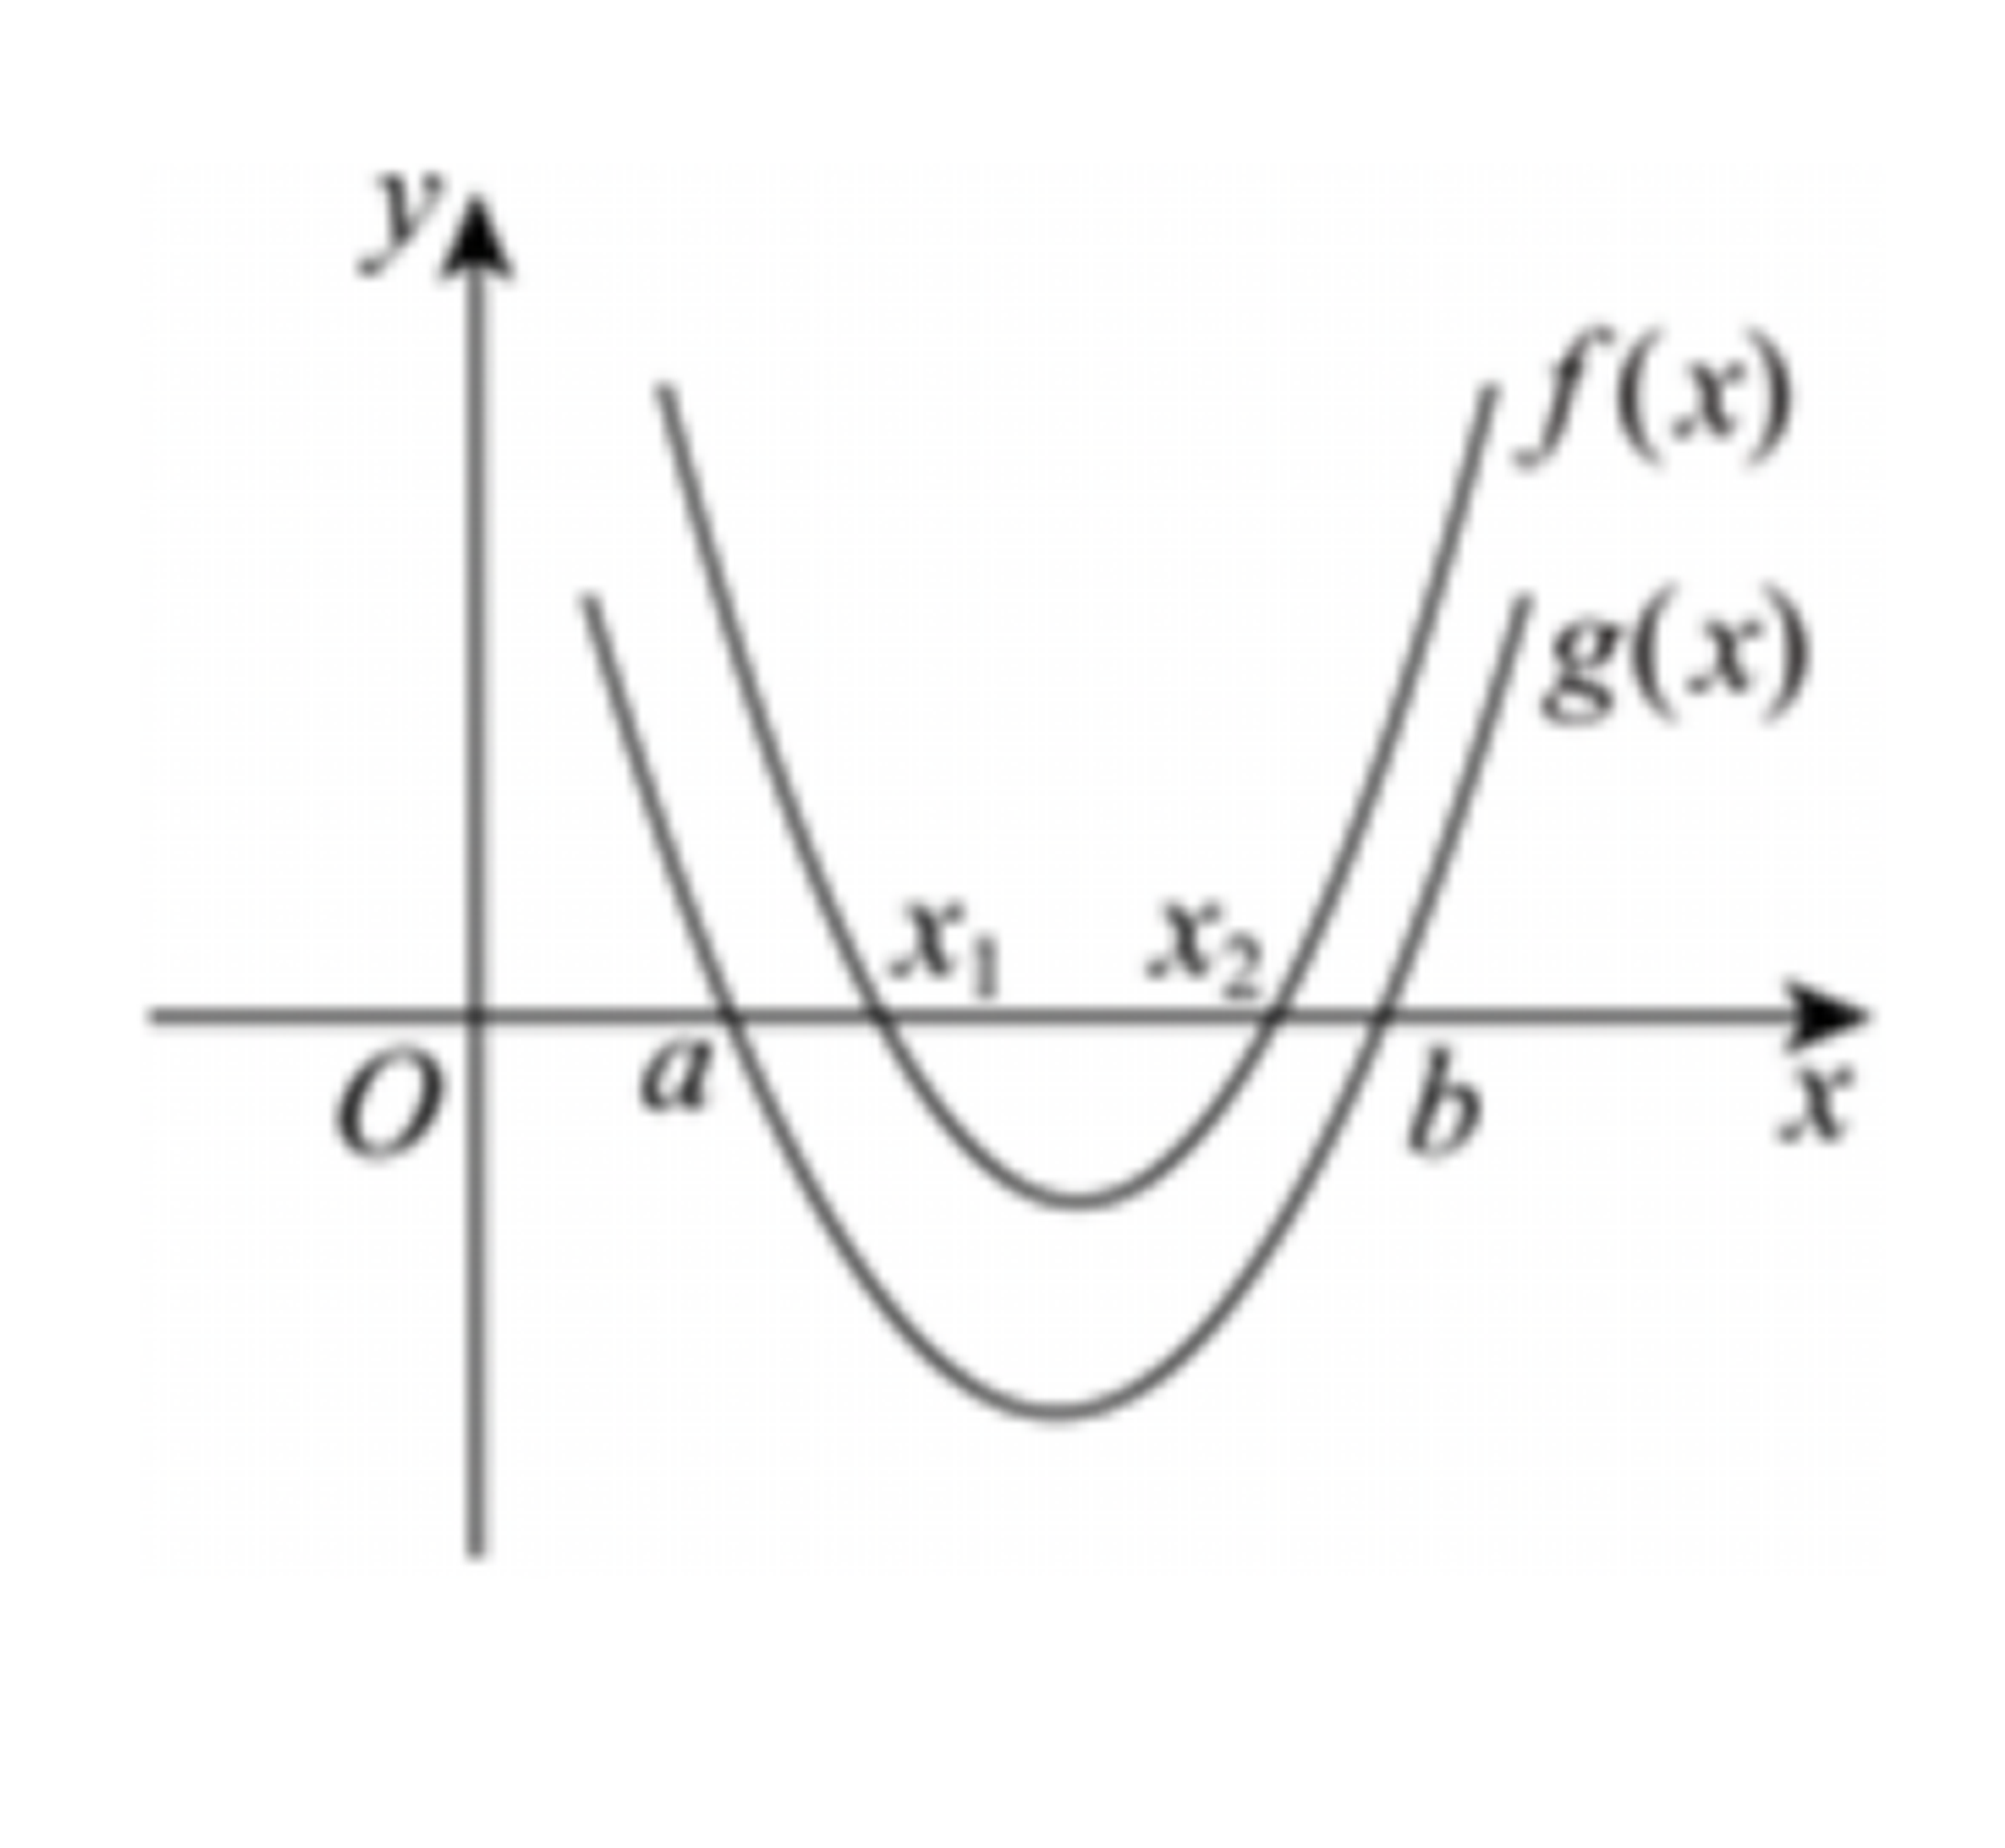
\includegraphics[width=0.30\textwidth]{figures/parabola_f_g_x1x2_h65.png}
\end{center}
\step{由图像得 $a<x_1<x_2<b$，故选 $B$.}
\solend
\fi

\end{enumerate}

\bigsec{三、解答题}

\begin{enumerate}
\setcounter{enumi}{16}

\item 已知 $a>0$，$b>0$，若 $a+b>4$，求证：$\dfrac a{b+2}$ 和 $\dfrac b{a+2}$ 中至少有一个大于 $\dfrac12$.

\ifanswer
\solbegin
\step{假设 $\dfrac a{b+2}\leqslant\dfrac12$，$\dfrac b{a+2}\leqslant\dfrac12$，}
\step{$a>0$，$b>0$，则 $a+2>0$，$b+2>0$，故 $2a\leqslant b+2$，$2b\leqslant a+2$，}
\step{两式相加得 $a+b\leqslant4$，与 $a+b>4$ 矛盾，故 $\dfrac a{b+2}$ 和 $\dfrac b{a+2}$ 中至少有一个大于 $\dfrac12$.}
\solend
\fi

\ansspace[6]

\item 已知集合 $A=\{x\mid-4<x<5\}$，$B=\{x\mid x\leqslant a-6\text{ 或 }x\geqslant a+2\}$.

\begin{enumerate}[label=(\arabic*)]

\item 若 $A\cup B=\R$，求实数 $a$ 的取值范围；

\item 若“$x\in A$”是“$x\in B$”的充分不必要条件，求实数 $a$ 的取值范围.

\end{enumerate}

\ifanswer
\solbegin
\stepm{(1)}{集合 $A=\{x\mid-4<x<5\}$，$B=\{x\mid x\leqslant a-6\text{ 或 }x\geqslant a+2\}$.}
\step{由 $A\cup B=\R$ 得 $\begin{cases}a-6\geqslant-4\\ a+2\leqslant5\end{cases}$，解得 $2\leqslant a\leqslant3$，$a$ 的取值范围为 $[2,3]$；}
\stepm{(2)}{若“$x\in A$”是“$x\in B$”的充分不必要条件，则 $A\subset B$，}
\step{则 $5\leqslant a-6$ 或 $-4\geqslant a+2$，解得 $a\leqslant-6$ 或 $a\geqslant11$.}
\solend
\fi

\ansspace[8]

% 注：原卷题干把命题 $P$ 印作“$\exists3\notin A$”（多一个存在量词），而【解析】两处均作
%     “$3\notin A$”；照录未改，见文件头“原卷笔误/存疑”③。
\item 已知集合 $A=\left\{x\mid\dfrac{x-1}{x-m}<0\right\}$，集合 $B=\left\{x\mid\left|\dfrac{x-1}{x-3}\right|\geqslant1\right\}$，命题 $P$：“$\exists3\notin A$”，命题
$Q$：$A\cap B\neq\varnothing$.

\begin{enumerate}[label=(\arabic*)]

\item 若命题 $P$ 为真命题，求 $m$ 的取值范围；

\item 若命题 $P$ 和命题 $Q$ 至少有一个为假命题，求实数 $m$ 的取值范围.

\end{enumerate}

\ifanswer
\solbegin
\stepm{(1)}{$A=\left\{x\mid\dfrac{x-1}{x-m}<0\right\}=\{x\mid(x-1)(x-m)<0\}$，}
\step{若命题 $P$：“$3\notin A$”为真命题，则 $(3-1)(3-m)\geqslant0$，解得 $m\leqslant3$，}
\step{故实数 $m$ 的取值范围为 $(-\infty,3]$；}
\stepm{(2)}{$B=\left\{x\mid\left|\dfrac{x-1}{x-3}\right|\geqslant1\right\}$，由 $\left|\dfrac{x-1}{x-3}\right|\geqslant1$，得 $\begin{cases}|x-1|\geqslant|x-3|\\ x\neq3\end{cases}$，}
\step{等价于 $\begin{cases}(x-1)^2\geqslant(x-3)^2\\ x\neq3\end{cases}$，解得 $x\geqslant2$ 且 $x\neq3$，所以 $B=[2,3)\cup(3,+\infty)$，}
\step{因为 $A=\{x\mid(x-1)(x-m)<0\}$，}
\step{当 $m=1$ 时，$A=\varnothing$，不满足 $A\cap B\neq\varnothing$，}
\step{当 $m<1$ 时，$A=(m,1)$，不满足 $A\cap B\neq\varnothing$，}
\step{当 $m>1$ 时，$A=(1,m)$，要使 $A\cap B\neq\varnothing$，则 $m>2$，}
\step{则若命题 $Q$：“$A\cap B\neq\varnothing$”为真命题时，实数 $m$ 的取值范围为 $(2,+\infty)$，}
\step{当命题 $P$ 与命题 $Q$ 都是真命题时，则 $\begin{cases}m\leqslant3\\ m>2\end{cases}$，解得 $2<m\leqslant3$，}
\step{则命题 $P$ 和命题 $Q$ 至少有一个为假命题时，得 $m\leqslant2$ 或 $m>3$，}
\step{故实数 $m$ 的取值范围为 $(-\infty,2]\cup(3,+\infty)$.}
\solend
\fi

\ansspace[8]

\item 已知函数 $y=ax^2-(a+2)x+2$，$a\in\R$.

\begin{enumerate}[label=(\arabic*)]

\item $y<3-2x$ 恒成立，求实数 $a$ 的取值范围；

% 注：原卷末句作“求实数 $a$ 的取值”（疑脱“范围”二字），照录未改，
%     见文件头“原卷笔误/存疑”⑤。
\item 若存在 $m>0$ 使关于 $x$ 的方程 $ax^2-(a+2)|x|+2=m+\dfrac1m+1$ 有四个不同的实根，
求实数 $a$ 的取值.

\end{enumerate}

\ifanswer
\solbegin
\stepm{(1)}{由题意得 $ax^2-(a+2)x+2<3-2x$ 恒成立，}
\step{即 $ax^2-ax-1<0$ 恒成立，}
\step{当 $a=0$ 时，$-1<0$ 恒成立，符合题意，}
\step{当 $a\neq0$ 时，则 $\begin{cases}a<0\\ \triangle=a^2+4a<0\end{cases}$，得 $\begin{cases}a<0\\ -4<a<0\end{cases}$，得 $-4<a<0$，}
\step{综上，$a$ 的取值范围为 $(-4,0]$.}
\stepm{(2)}{当 $m>0$ 时，令 $t=m+\dfrac1m+1\geqslant2\sqrt{m\times\dfrac1m}+1=3$，}
\step{当且仅当 $m=1$ 时取等号，}
% 注：题干只给“函数 $y=ax^2-(a+2)x+2$”，全卷未设 $f$，此处 $f(|x|)$ 无定义；
%     照录未改，见文件头“原卷笔误/存疑”④。
\step{则关于 $x$ 的方程 $f(|x|)=t$ 可化为 $a|x|^2-(a+2)|x|+2-t=0$，}
\step{关于 $x$ 的方程为 $a|x|^2-(a+2)|x|+2-t=0$ 有四个不等的实数根，}
\step{即 $ax^2-(a+2)x+2-t=0$，有两个不同的实数正根，}
\step{则 $\begin{cases}\triangle=(a+2)^2-4a(2-t)>0\\ \dfrac{a+2}a>0\\ \dfrac{2-t}a>0\end{cases}$，解得 $a<-2$，}
\step{由（1）得存在 $t\in[3,+\infty)$ 使得不等式 $4at+(a+2)^2-8a>0$ 成立，}
\step{故 $4a\times3+(a+2)^2-8a>0$，即 $a^2+8a+4>0$，}
\step{解得 $a<-4-2\sqrt3$ 或 $a>-4+2\sqrt3$，}
\step{综上，$a<-4-2\sqrt3$，所以 $a$ 的取值范围为 $(-\infty,-4-2\sqrt3)$.}
\solend
\fi

\ansspace[8]

\item 若集合 $A=B_1\cup B_2\cup\cdots\cup B_n$，其中 $B_1$、$B_2$、$\cdots$、$B_n$ 为非空集合，
$B_i\cap B_j=\varnothing$($1\leqslant i<j\leqslant n$)，则称集合 $\{B_1,B_2,\cdots,B_n\}$ 为集合 $A$ 的一个 $n$ 划分.

\begin{enumerate}[label=(\arabic*)]

\item 写出集合 $A=\{1,2,3\}$ 的所有不同的 2 划分；

\item 设 $\{B_1,B_2\}$ 为有理数集 $\Q$ 的一个 2 划分，且满足对任意 $x\in B_1$，任意 $y\in B_2$，都有
$x<y$，判断命题“$B_1$ 中的元素存在最大值，$B_2$ 中的元素存在最小值.”的真假，并说明
理由.

\item 设集合 $A=\{1,2,3,\cdots,16\}$，对于集合 $A$ 的任意一个 3 划分 $\{B_1,B_2,B_3\}$，判断是否存
在 $i\in\{1,2,3\}$，存在 $a$、$b\in B_i$，使得 $b-a\in B_i$ 成立，并说明理由.

\end{enumerate}

\ifanswer
\solbegin
% 注：原卷三个“2 划分”本有外层花括号（$\{\{1,2\},\{3\}\}$ 等），首轮误脱；
%     第二轮复核照原卷补回（原卷原样 / 本稿原错处：原脱外层花括号）。
\stepm{(1)}{集合 $A=\{1,2,3\}$ 的所有不同的 2 划分为 $\{\{1,2\},\{3\}\}$、$\{\{1,3\},\{2\}\}$、}
\step{$\{\{2,3\},\{1\}\}$.}
\stepm{(2)}{该命题为假命题，理由如下：}
\step{假设命题为真，则不妨设 $B_1$ 中元素的最大值为 $s$，$B_2$ 中元素的最小值为 $t$，}
\step{由题意得 $s<t$，所以 $s<\dfrac{s+t}2<t$，}
\step{因为 $s$ 为 $B_1$ 中元素的最大值，所以 $\dfrac{s+t}2\notin B_1$，}
\step{因为 $t$ 为 $B_2$ 中元素的最小值，所以 $\dfrac{s+t}2\notin B_2$，}
\step{因为 $B_1\cup B_2=\Q$，所以 $\dfrac{s+t}2\notin\Q$，}
\step{这与 $\dfrac{s+t}2\in\Q$ 矛盾，所以假设不成立，即命题不可能成立；}
\stepm{(3)}{由于集合 $A$ 中有 16 个元素，}
\step{所以 $B_1$、$B_2$、$B_3$ 中至少有一个集合至少包含 6 个元素，}
\step{不妨设 $B_1$ 中至少包含 6 个元素，}
\step{设 $b_1$、$b_2$、$b_3$、$b_4$、$b_5$、$b_6\in B_1$，且 $b_1<b_2<b_3<b_4<b_5<b_6$，}
\step{假设对任意 $i\in\{1,2,3\}$，对任意 $a$、$b\in B_i$，都有 $b-a\notin B_i$，}
\step{那么 $b_6-b_1$、$b_6-b_2$、$b_6-b_3$、$b_6-b_4$、$b_6-b_5\notin B_1$，}
\step{又因为 $b_6-b_1$、$b_6-b_2$、$b_6-b_3$、$b_6-b_4$、$b_6-b_5\in A$，}
\step{所以 $b_6-b_1$、$b_6-b_2$、$b_6-b_3$、$b_6-b_4$、$b_6-b_5\in B_2\cup B_3$，}
\step{则 $B_2$、$B_3$ 中必有一个集合}
\step{至少包含 $b_6-b_1$、$b_6-b_2$、$b_6-b_3$、$b_6-b_4$、$b_6-b_5$ 中的 3 个元素，}
\step{不妨设这 3 个元素为 $a_1$、$a_2$、$a_3\in B_2$，$a_1<a_2<a_3$，}
\step{由假设得 $a_3-a_1$、$a_3-a_2$、$a_2-a_1\notin B_2$，}
\step{对任意 $i$、$j$($1\leqslant j<i\leqslant3$)，存在 $m$、$n$($1\leqslant m<n\leqslant5$)，}
\step{都有 $a_i-a_j=b_6-b_m-b_6+b_n=b_n-b_m\notin B_1$，}
\step{又因为 $a_3-a_1$、$a_3-a_2$、$a_2-a_1\in B_3$，而 $a_3-a_1-(a_3-a_2)=a_2-a_1$，}
\step{与假设矛盾，所以假设不成立，}
\step{即存在 $i\in\{1,2,3\}$，存在 $a$、$b\in B_i$，使得 $b-a\in B_i$.}
\solend
\fi

\ansspace*[10]

\end{enumerate}

\end{document}
"
% 紧凑版：xelatex "\def\iscompact{1}% 高一65_大同中学_10月月考.tex
%   —— 高一上数学“2026-2027 年大同中学高一上 10 月月考”（讲评版）
% 试卷版：xelatex 高一65_大同中学_10月月考.tex
% 答案版：xelatex "\def\isanswer{1}\input{高一65_大同中学_10月月考.tex}"
% 紧凑版：xelatex "\def\iscompact{1}\input{高一65_大同中学_10月月考.tex}"
%
% 原始材料：微信公众号“魔都数学加油站”文章，作者破晓，连载“27学年高一65”；
% 原文标题“27学年高一65——2026-2027年上海市大同中学高一上10月月考”；
% 原文链接：https://mp.weixin.qq.com/s/h9ctuk-ByE1Vfg2Rx2C6bw。
% 页面标注发布时间 2026-10-17 21:58（上海）。
% 本次转录只据 `原图/高一65_大同中学_10月月考/` 的 11 张 PNG 逐页读图。
% 正文为 11 张 PNG 页（`01..11.png`）：
% 第 06、11 页 2560×3620，第 01、02、03、04、05、07、08、09、10 页 4762×6735
% （**同一篇各页分辨率不同**），均按页序读取。11 页全为试卷正文页（卷首标题在第 1 页页顶，
% 卷末解答题第 21 题解析止于第 11 页），无封面页、目录页、二维码或宣传页。
% 粉色斜排“魔都数学加油站”为卷面水印，与公众号页脚一并未录入。
%
% 卷首标题：照卷面印作“2026--2027 年大同中学高一上 10 月月考”，年份区间按全稿惯例排 en dash。
% 原卷只有一行标题、无副标题。
%
% 篇幅与题号：原卷自第 3 题起编号（第 1、2 题不在本卷内）。填空题 3—12（10 题）、
% 选择题 13—16（4 题）、解答题 17—21（5 题），共 19 题。本稿沿用原节与原题号，
% 只改排为全稿统一的大节样式（原卷小节标题为“一、填空题”“二、选择题”“三、解答题”）。
%
% 讲评版：原卷每题下直接印【答案】或【解析】。**只印【答案】的 4 题**（第 3、4、7、10 题），
% 本稿只给 \ans{}；其余 15 题都印【解析】（按全稿口径这类题不另提 \ans{}——第 12、13、14、
% 15、16 题的结论写在解析末句（“故选 B”“综上，n 的最大值为 14”等），亦照录在解析内）。
% 全卷无“答案印在题干括号内”的题（第 13—16 题的选择题括号内均空白）。
%
% 副标题：原卷未印副标题。本稿按“知识模块”口径标作“集合与常用逻辑用语、不等式”：
% 19 题中集合与常用逻辑用语 10 题（第 3、4、6、8、12、14、15、18、19、21 题），
% 不等式 9 题（含等式恒等、不等式性质、二次不等式、恒成立、基本不等式、不等式的证明：
% 第 5、7、9、10、11、13、16、17、20 题），两类均超过三分之一，故并标。口径同 高一63。
%
% 与原卷的排版差异：
%   ① 原卷每题下直接印【答案】/【解析】，本稿按全稿惯例将答案与解析置于答案版，试卷版保持干净；
%   ② 原卷未印副标题，本稿按“知识模块”口径补出；
%   ③ 原卷填空横线约四个字宽，本稿按全稿惯例统一排 \blankline[4.4em]；
%   ④ 原卷数集记号全为斜体：实数集作 $R$（第 6 题两处、第 8 题两处、第 15 题解析、第 18 题、
%      第 20 题题干），自然数集作 $N$（第 12 题题干“$n\in N,n\geqslant1$”），有理数集作 $Q$
%      （第 21 题 (2) 题干与解析共 4 处），本稿按全稿惯例统一改用 $\R$、$\N$、$\Q$
%      （同 高一63 排版差异④：记号归一）；空集记号原卷作 $\varnothing$，照录；
%   ⑤ 原卷用描述法时竖线排细竖“$|$”（如 $\{x|0<x<3\}$、$\{x|(x-1)(x-m)<0\}$），
%      本稿按全稿惯例排 \mid；
%   ⑥ 原卷判别式印作“$\triangle$”（第 8、14 题解析各 1 处、第 20 题解析 2 处，共 4 处），
%      本稿照录用 \triangle（同 高一39 成例），未改作 \Delta；
%   ⑦ 第 18—21 题的子问原卷各自另起一行、以“（1）”“（2）”标号，本稿按全稿惯例用
%      enumerate 的 (1)(2)(3)；解析中的子问标号一律用 \stepm{(1)}{…}；
%      第 18—21 题解析（原文以“（1）”“（2）”“（3）”冠于解析首句）同此；
%   ⑧ 选择题的作答括号原卷排半角“(　　)”（第 13—16 题括号内均空白），
%      本稿按全稿惯例排 \mbox{（\quad）}；选项字母后的句点照原卷排“A.”“B.”；
%   ⑨ 每道解答题原卷未留作答空白，本稿按全稿惯例加 \ansspace（末题用 \ansspace*）；
%   ⑩ 原卷在数学式内多处用半角逗号（如 $\{x|0<x<3\},B=\{x|x>2\}$、$m\in I_{14},k\in I_{14}$），
%      均照录未强改；句末句点按全稿惯例排西文句点。
%
% 原卷笔误/存疑（均照录未改，正文对应处另有 % 注）：
%   ① 第 13 题题干“下列不等式中一定成立是（　　）”脱一个“的”（当作“一定成立的是”），
%      8 倍放大确认非水印遮挡，本稿照录；
%   ② 第 15 题【解析】末段把题干条件“$x\geqslant10$”写成“$x\geqslant1$”
%      （“所以 $x+2+\frac{16}{x+2}(x\geqslant1)$ 的最小值不为 8”），与同段前面“令 $t=x+2$，
%      则 $t\geqslant12$”不合，本稿照录；
%   ③ 第 19 题题干把命题 $P$ 印作“$\exists3\notin A$”（多一个存在量词），而【解析】两处
%      均作“$3\notin A$”，前后记号不一，本稿照录；
%   ④ 第 20 题【解析】(2) 出现 $f(|x|)$，但题干只给“函数 $y=ax^2-(a+2)x+2$”、全卷未设 $f$，
%      本稿照录；
%   ⑤ 第 20 题 (2) 题干末句作“求实数 $a$ 的取值”（疑脱“范围”二字），本稿照录；
%   ⑥ 第 12 题【解析】第 18 步“它与 $P_n$ 中的任何其他数之和都不是整数”，该段所论为 $P_{14}$
%      （前后均作 $P_{14}$），此处 $P_n$ 疑当作 $P_{14}$，本稿照录。
%
% 第二轮复核（2026-10-18）订正「本稿抄错原卷」一处：
%   第 21 题 (1)【解析】原卷本作“$\{\{1,2\},\{3\}\}$、$\{\{1,3\},\{2\}\}$、$\{\{2,3\},\{1\}\}$”，
%   有外层花括号；首轮误脱外层花括号，并曾在文件头误记为“原卷未加外层花括号”（原第 ⑦ 条，
%   已撤销）。本次照原卷补回，正文对应处另有 % 注。
%
% 插图：第 16 题【解析】内有 1 幅图（两条开口向上的抛物线 $f(x)$、$g(x)$ 与 $x$ 轴交点
% 标 $a$、$x_1$、$x_2$、$b$，纵轴标 $y$、原点 $O$），解析第三行“画出函数 $g(x)$ 与函数 $f(x)$
% 的图像，如图所示”即指此图；取原卷截图（06.png，2560×3620）右半幅，4× LANCZOS 放大，
% 存 figures/parabola_f_g_x1x2_h65.png。该图在【解析】内，仅答案版出。
%
\documentclass[a4paper,11pt]{article}
\usepackage{common}

\begin{document}

\examtitlest[3]{2026--2027 年大同中学高一上 10 月月考}{集合与常用逻辑用语、不等式}

\bigsec{一、填空题}

\begin{enumerate}
\setcounter{enumi}{2}

\item 已知集合 $A=\{x\mid0<x<3\}$,$B=\{x\mid x>2\}$，则集合 $A\cup B=$\blankline[4.4em].

\ifanswer
\ans{$(0,+\infty)$}
\fi

\item “$x>1$ 或 $y>1$”的否定形式是\blankline[4.4em].

\ifanswer
\ans{$x\leqslant1$ 且 $y\leqslant1$}
\fi

\item 已知等式 $2x^2+3x+4=a(2x+1)(x+1)+b$ 恒成立，则常数 $a-b=$\blankline[4.4em].

\ifanswer
\solbegin
\step{因为等式 $2x^2+3x+4=a(2x+1)(x+1)+b$ 恒成立，}
\step{所以 $a(2x+1)(x+1)+b=2ax^2+3ax+a+b=2x^2+3x+4$，}
\step{所以 $\begin{cases}2a=2\\ 3a=3\\ a+b=4\end{cases}$，解得 $\begin{cases}a=1\\ b=3\end{cases}$，所以 $a-b=-2$.}
\solend
\fi

\item 全集为 $U=\R$，$A=\{x\mid|x|\geqslant2\}$，$B=\{y\mid y=x^2+1,x\in\R\}$，则 $A\cup\bar B=$\blankline[4.4em].

\ifanswer
\solbegin
\step{由题意得集合 $A=\{x\mid x\geqslant2\text{ 或 }x\leqslant-2\}$，}
\step{因为 $x^2+1\geqslant1$，所以集合 $B=\{x\mid x\geqslant1\}$，所以 $\bar B=\{x\mid x<1\}$，}
\step{则 $A\cup\bar B=\{x\mid x\geqslant2\text{ 或 }x<1\}$.}
\solend
\fi

\item 已知 $|x+3|+|x-5|=8$，则实数 $x$ 的取值范围为\blankline[4.4em].

\ifanswer
\ans{$[-3,5]$}
\fi

\item 已知集合 $A=\{x\in\R\mid ax^2+2x+1=0,a\in\R\}$ 只有一个元素，则 $a$ 的值为\blankline[4.4em].

\ifanswer
\solbegin
\step{当 $a=0$ 时，$A=\left\{-\dfrac12\right\}$；}
\step{当 $a\neq0$ 时，若集合 $A$ 只有一个元素，由 $\triangle=4-4a=0$ 得 $a=1$.}
\step{综上，当 $a=0$ 或 $a=1$ 时，集合 $A$ 只有一个元素.}
\solend
\fi

\item 已知不等式 $-x^2+bx+c>0$ 的解集为 $(3,4)$，则不等式 $cx^2+bx-1<0$ 的解集为\blankline[4.4em].

\ifanswer
\solbegin
\step{由题意得 3，4 是方程 $-x^2+bx+c=0$ 的两个实数根，}
\step{所以 $\begin{cases}3+4=b\\ 3\times4=-c\end{cases}$，得 $b=7$，$c=-12$，}
\step{则不等式 $cx^2+bx-1<0$，即为 $-12x^2+7x-1<0$，即 $12x^2-7x+1>0$，}
\step{化简得 $(3x-1)(4x-1)>0$，解得 $x<\dfrac14$ 或 $x>\dfrac13$，}
\step{即不等式 $cx^2+bx-1<0$ 的解集为 $\left(-\infty,\dfrac14\right)\cup\left(\dfrac13,+\infty\right)$.}
\solend
\fi

\item 对于区间 $(m,n)$，我们将 $n-m$ 的值称为该区间的长度. 若关于 $x$ 的不等式
$x^2+ax+a<0$ 有解，且解集的区间长度不超过 $2\sqrt3$，则实数 $a$ 的取值范围是\blankline[4.4em].

\ifanswer
\ans{$[-2,0)\cup(4,6]$}
\fi

\item 当 $x>0$ 时，关于 $x$ 的不等式 $(ax-1)(x^2+bx-4)\geqslant0$ 恒成立，则 $b+\dfrac2a$ 的最小值
为\blankline[4.4em].

\ifanswer
\solbegin
\step{由题意 $a\neq0$；}
\step{若 $a<0$，则 $x>0$ 时 $ax-1<0$ 恒成立，需 $x^2+bx-4\leqslant0$ 对一切 $x>0$ 成立，}
\step{而 $y=x^2+bx-4$ 的图象开口向上，当 $x$ 充分大时必为正值，矛盾，故 $a>0$.}
\step{当 $a>0$ 时，$ax-1=a\left(x-\dfrac1a\right)$，故原条件化为 $\left(x-\dfrac1a\right)(x^2+bx-4)\geqslant0$：}
\step{若 $0<x<\dfrac1a$，则 $x-\dfrac1a<0$，需 $x^2+bx-4\leqslant0$；}
\step{若 $x>\dfrac1a$，则 $x-\dfrac1a>0$，需 $x^2+bx-4\geqslant0$；}
\step{由 $y=x^2+bx-4$ 的连续性知 $x=\dfrac1a$ 是它的零点，}
\step{即 $\dfrac1{a^2}+\dfrac ba-4=0$，得 $b=4a-\dfrac1a$；}
\step{此时 $x^2+bx-4=x^2+\left(4a-\dfrac1a\right)x-4=(x+4a)\left(x-\dfrac1a\right)$，}
\step{由 $a>0$、$x>0$ 得 $x+4a>0$，}
\step{其符号与 $x-\dfrac1a$ 一致，故能与 $ax-1$ 同号，原不等式确在 $x>0$ 上恒成立.}
\step{于是 $b+\dfrac2a=4a-\dfrac1a+\dfrac2a=4a+\dfrac1a\geqslant2\sqrt{4a\cdot\dfrac1a}=4$，}
\step{当且仅当 $a=\dfrac12$ 时取等号，故最小值为 4.}
\solend
\fi

\item 设集合 $I_n=\{1,2,\cdots,n\}$，$n\in\N$，$n\geqslant1$，集合 $P_n=\left\{\dfrac m{\sqrt k}\mid m\in I_n,k\in I_n\right\}$，若 $P_n$ 的子集 $A$
中任意两个元素之和不是整数的平方，则称 $A$ 为“人文集”. 那么使 $P_n$ 能分成两个交集为空
集的“人文集”的并集，且这两个人文集的并集恰为 $P_n$ 时，$n$ 的最大值是\blankline[4.4em].

\ifanswer
\solbegin
\step{先证当 $n\geqslant15$ 时，$P_n$ 不能分成两个不相交的人文集的并集.}
\step{假设当 $n\geqslant15$ 时，$P_n$ 可以分成两个不相交的人文集的并集，}
\step{设 $A$ 和 $B$ 为两个不相交的人文集，使 $A\cup B=P_n\supseteq I_n$.}
\step{不妨设 $1\in A$，则由于 $1+3=2^2$，所以 $3\notin A$，即 $3\in B$.}
\step{同理可得，$6\in A$，$10\in B$. 又推出 $15\in A$，}
\step{但 $1+15=4^2$，这与 $A$ 为人文集相矛盾.}
\step{再证 $P_{14}$ 满足要求. 当 $k=1$ 时，$P_{14}=\left\{\dfrac m{\sqrt k}\mid m\in I_{14},k\in I_{14}\right\}$，}
\step{可以分成 2 个人文集的并集.}
\step{事实上，只要取 $A_1=\{1,2,4,6,9,11,13\}$，$B_1=\{3,5,7,8,10,12,14\}$，}
\step{则 $A_1$ 和 $B_1$ 都是人文集，且 $A_1\cup B_1=P_{14}$.}
\step{当 $k=4$ 时，集合 $\left\{\dfrac m{\sqrt k}\mid m\in I_{14}\right\}$ 中，除整数外，}
\step{剩下的数组成集合 $\left\{\dfrac12,\dfrac32,\dfrac52,\cdots,\dfrac{13}2\right\}$，}
\step{可以分为下列 2 个人文集的并：$A_2=\left\{\dfrac12,\dfrac52,\dfrac92,\dfrac{11}2\right\}$，$B_2=\left\{\dfrac32,\dfrac72,\dfrac{13}2\right\}$.}
\step{当 $k=9$ 时，集合 $\left\{\dfrac m{\sqrt k}\mid m\in I_{14}\right\}$ 中，除整数外，}
\step{剩下的数组成集合 $\left\{\dfrac13,\dfrac23,\dfrac43,\dfrac53,\cdots,\dfrac{13}3,\dfrac{14}3\right\}$，}
\step{可以分为下列 2 个人文集的并：$A_3=\left\{\dfrac13,\dfrac43,\dfrac53,\dfrac{10}3,\dfrac{13}3\right\}$，$B_3=\left\{\dfrac23,\dfrac73,\dfrac83,\dfrac{11}3,\dfrac{14}3\right\}$.}
\step{最后，集合 $C=\left\{\dfrac m{\sqrt k}\mid m\in I_{14},k\in I_{14},k\neq1,4,9\right\}$ 中的数的分母都是无理数，}
% 注：本行原卷作“$P_n$”，而该段所论为 $P_{14}$（前后均作 $P_{14}$），疑当作 $P_{14}$；
%     照录未改，见文件头“原卷笔误/存疑”⑥。
\step{它与 $P_n$ 中的任何其他数之和都不是整数，}
\step{因此，令 $A=A_1\cup A_2\cup A_3\cup C$，$B=B_1\cup B_2\cup B_3$，}
\step{则 $A$ 和 $B$ 是不相交的人文集，且 $A\cup B=P_{14}$.}
\step{综上，$n$ 的最大值为 14.}
\solend
\fi

\end{enumerate}

\bigsec{二、选择题}

\begin{enumerate}
\setcounter{enumi}{12}

% 注：原卷题干“下列不等式中一定成立是”脱一个“的”（当作“一定成立的是”），
%     照录未改，见文件头“原卷笔误/存疑”①。
\item 已知 $a>b$，下列不等式中一定成立是\mbox{（\quad）}

\keepwithprev
A. $a^2>b^2$\qquad B. $ac^2>bc^2$\qquad C. $\dfrac1a<\dfrac1b$\qquad D. $a+3>b-4$

\ifanswer
\solbegin
\step{对于 $A$，当 $a=-2$，$b=-4$ 时，不等式不成立，故 $A$ 错误；}
\step{对于 $B$，当 $c=0$ 时，不等式不成立，故 $B$ 错误；}
\step{对于 $C$，当 $a=2$，$b=-4$ 时，不等式不成立，故 $C$ 错误；}
\step{对于 $D$，因为 $a>b$，$3>-4$，必有 $a+3>b-4$ 成立，故 $D$ 正确.}
\step{故选 $D$.}
\solend
\fi

\item 已知 $a$ 为实数，那么“$|a|\leqslant2$”是“方程 $x^2+ax+1=0$ 没有实数解”的\mbox{（\quad）}

\keepwithprev
A. 充分而不必要条件\qquad B. 必要而不充分条件

C. 充要条件\qquad D. 既不充分也不必要条件

\ifanswer
\solbegin
\step{由方程 $x^2+ax+1=0$ 没有实数解，得 $\triangle=a^2-4<0$，则 $|a|<2$，}
\step{由 $|a|<2$ 得 $|a|\leqslant2$，反之不成立，}
\step{所以“$|a|\leqslant2$”是“方程 $x^2+ax+1=0$ 没有实数解”的必要而不充分条件.}
\step{故选 $B$.}
\solend
\fi

\item 下列命题为真命题的是\mbox{（\quad）}

\keepwithprev
A. $a>b>0$，当 $m>0$ 时，$\dfrac{a+m}{b+m}>\dfrac ab$

B. 集合 $A=\{x\mid y=x^2+1\}$ 与集合 $B=\{y\mid y=x^2+1\}$ 是相同的集合

C. 若 $b<a<0$，$m<0$，则 $\dfrac ma>\dfrac mb$

D. $x+2+\dfrac{16}{x+2}(x\geqslant10)$ 最小值为 8

\ifanswer
\solbegin
\step{对于 $A$，$\dfrac{a+m}{b+m}-\dfrac ab=\dfrac{b(a+m)-a(b+m)}{b(b+m)}=\dfrac{m(b-a)}{b(b+m)}$，}
\step{因为 $a>b>0$，$m>0$，所以 $b(b+m)>0$，$m(b-a)<0$，}
\step{所以 $\dfrac{a+m}{b+m}-\dfrac ab=\dfrac{m(b-a)}{b(b+m)}<0$，}
\step{即 $a>b>0$，当 $m>0$ 时，$\dfrac{a+m}{b+m}<\dfrac ab$，故 $A$ 错误；}
\step{对于 $B$，集合 $A=\{x\mid y=x^2+1\}=\R$，集合 $B=\{y\mid y=x^2+1\}=\{y\mid y\geqslant1\}$，}
\step{所以 $A\neq B$，故 $B$ 错误；}
\step{对于 $C$，$\dfrac ma-\dfrac mb=\dfrac{m(b-a)}{ab}$，}
\step{因为 $b<a<0$，$m<0$，所以 $ab>0$，$m(b-a)>0$，}
\step{所以 $\dfrac ma-\dfrac mb=\dfrac{m(b-a)}{ab}>0$，即 $\dfrac ma>\dfrac mb$，故 $C$ 正确；}
\step{对于 $D$，令 $t=x+2$，则 $t\geqslant12$，表达式变为 $t+\dfrac{16}t$，}
\step{$t+\dfrac{16}t\geqslant2\sqrt{t\cdot\dfrac{16}t}=8$，当且仅当 $t=4$ 时取等号，即等号不成立，}
% 注：原卷本行把题干条件“$x\geqslant10$”写成“$x\geqslant1$”，与同段“$t\geqslant12$”不合；
%     照录未改，见文件头“原卷笔误/存疑”②。
\step{所以 $x+2+\dfrac{16}{x+2}(x\geqslant1)$ 的最小值不为 8，故 $D$ 错误.}
\step{故选 $C$.}
\solend
\fi

\item 已知实数 $a<b$，关于 $x$ 的不等式 $x^2-(a+b)x+ab+\dfrac12<0$ 的解集为 $(x_1,x_2)$，则实数 $a$、
$b$、$x_1$、$x_2$ 从小到大的排列是\mbox{（\quad）}

\keepwithprev
A. $x_1<a<b<x_2$\qquad B. $a<x_1<x_2<b$\qquad C. $a<x_1<b<x_2$\qquad D. $x_1<a<x_2<b$

\ifanswer
\solbegin
\step{不等式 $x^2-(a+b)x+ab+\dfrac12<0$ 可化为 $(x-a)(x-b)+\dfrac12<0$，}
\step{设 $g(x)=(x-a)(x-b)$，$f(x)=g(x)+\dfrac12$，}
\step{画出函数 $g(x)$ 与函数 $f(x)$ 的图像，如图所示，}
% 图在【解析】内（仅答案版出），取原卷截图（06.png，2560×3620）右半幅，4× LANCZOS 放大。
\begin{center}
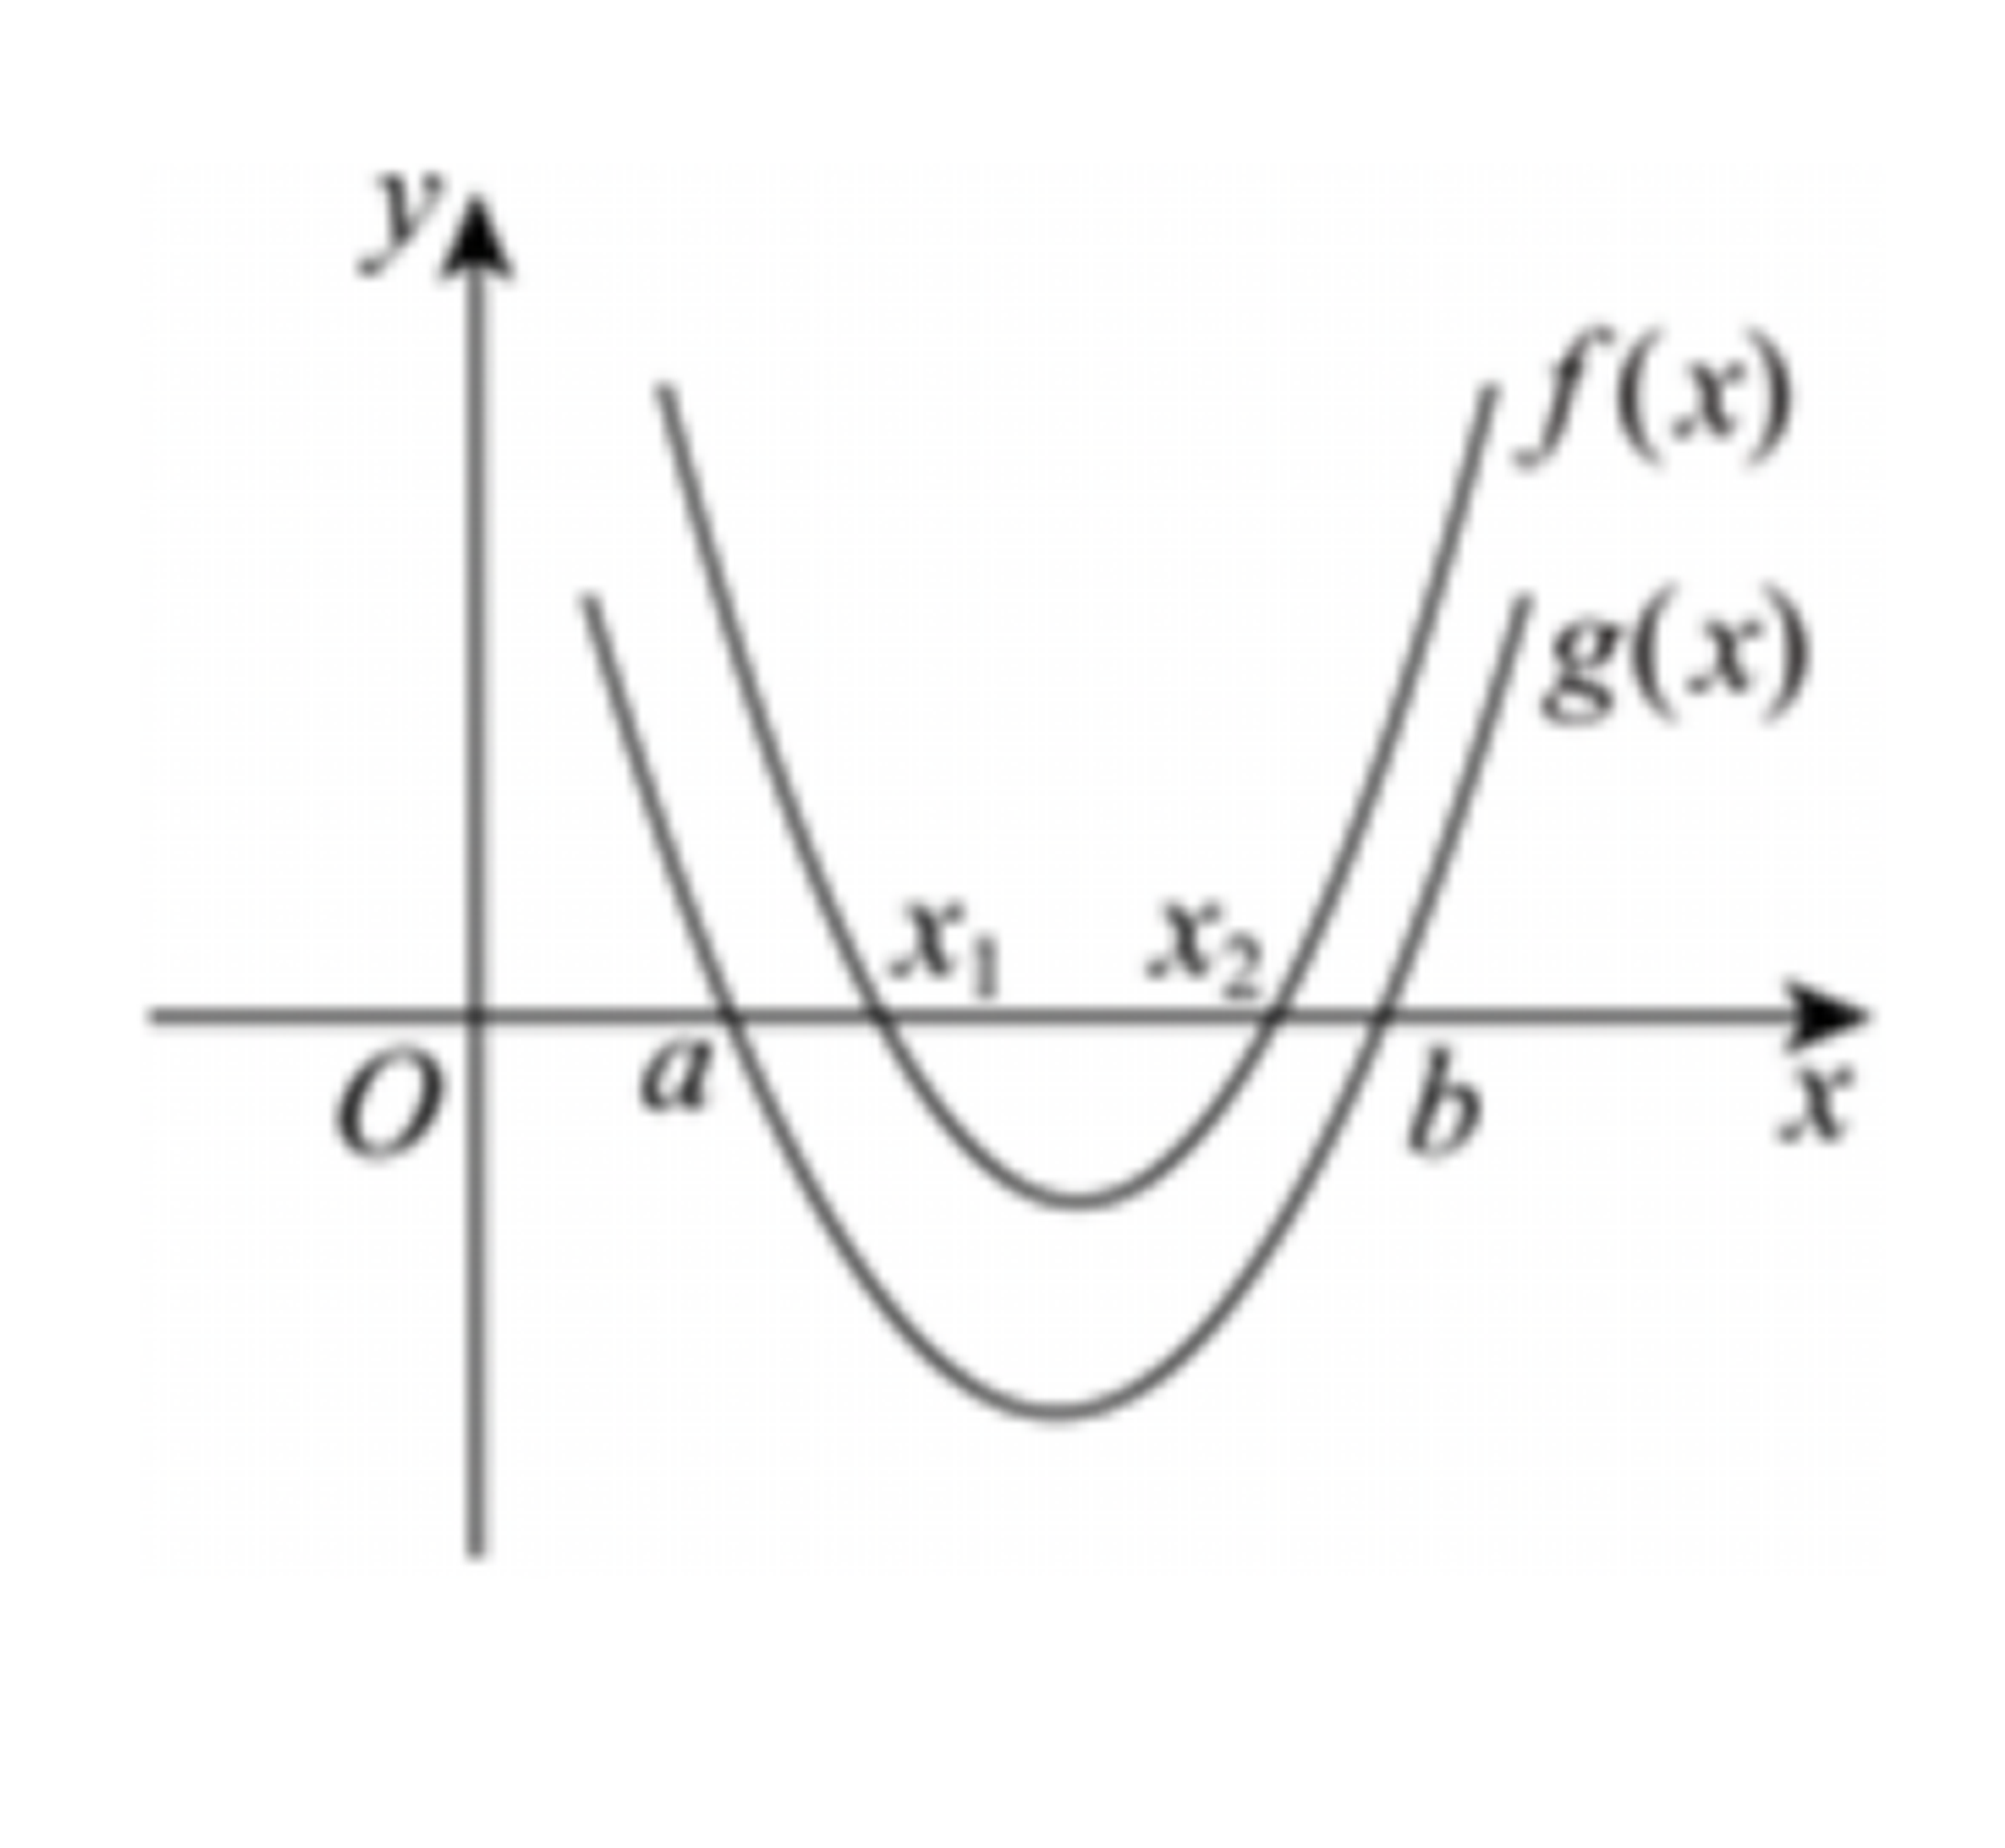
\includegraphics[width=0.30\textwidth]{figures/parabola_f_g_x1x2_h65.png}
\end{center}
\step{由图像得 $a<x_1<x_2<b$，故选 $B$.}
\solend
\fi

\end{enumerate}

\bigsec{三、解答题}

\begin{enumerate}
\setcounter{enumi}{16}

\item 已知 $a>0$，$b>0$，若 $a+b>4$，求证：$\dfrac a{b+2}$ 和 $\dfrac b{a+2}$ 中至少有一个大于 $\dfrac12$.

\ifanswer
\solbegin
\step{假设 $\dfrac a{b+2}\leqslant\dfrac12$，$\dfrac b{a+2}\leqslant\dfrac12$，}
\step{$a>0$，$b>0$，则 $a+2>0$，$b+2>0$，故 $2a\leqslant b+2$，$2b\leqslant a+2$，}
\step{两式相加得 $a+b\leqslant4$，与 $a+b>4$ 矛盾，故 $\dfrac a{b+2}$ 和 $\dfrac b{a+2}$ 中至少有一个大于 $\dfrac12$.}
\solend
\fi

\ansspace[6]

\item 已知集合 $A=\{x\mid-4<x<5\}$，$B=\{x\mid x\leqslant a-6\text{ 或 }x\geqslant a+2\}$.

\begin{enumerate}[label=(\arabic*)]

\item 若 $A\cup B=\R$，求实数 $a$ 的取值范围；

\item 若“$x\in A$”是“$x\in B$”的充分不必要条件，求实数 $a$ 的取值范围.

\end{enumerate}

\ifanswer
\solbegin
\stepm{(1)}{集合 $A=\{x\mid-4<x<5\}$，$B=\{x\mid x\leqslant a-6\text{ 或 }x\geqslant a+2\}$.}
\step{由 $A\cup B=\R$ 得 $\begin{cases}a-6\geqslant-4\\ a+2\leqslant5\end{cases}$，解得 $2\leqslant a\leqslant3$，$a$ 的取值范围为 $[2,3]$；}
\stepm{(2)}{若“$x\in A$”是“$x\in B$”的充分不必要条件，则 $A\subset B$，}
\step{则 $5\leqslant a-6$ 或 $-4\geqslant a+2$，解得 $a\leqslant-6$ 或 $a\geqslant11$.}
\solend
\fi

\ansspace[8]

% 注：原卷题干把命题 $P$ 印作“$\exists3\notin A$”（多一个存在量词），而【解析】两处均作
%     “$3\notin A$”；照录未改，见文件头“原卷笔误/存疑”③。
\item 已知集合 $A=\left\{x\mid\dfrac{x-1}{x-m}<0\right\}$，集合 $B=\left\{x\mid\left|\dfrac{x-1}{x-3}\right|\geqslant1\right\}$，命题 $P$：“$\exists3\notin A$”，命题
$Q$：$A\cap B\neq\varnothing$.

\begin{enumerate}[label=(\arabic*)]

\item 若命题 $P$ 为真命题，求 $m$ 的取值范围；

\item 若命题 $P$ 和命题 $Q$ 至少有一个为假命题，求实数 $m$ 的取值范围.

\end{enumerate}

\ifanswer
\solbegin
\stepm{(1)}{$A=\left\{x\mid\dfrac{x-1}{x-m}<0\right\}=\{x\mid(x-1)(x-m)<0\}$，}
\step{若命题 $P$：“$3\notin A$”为真命题，则 $(3-1)(3-m)\geqslant0$，解得 $m\leqslant3$，}
\step{故实数 $m$ 的取值范围为 $(-\infty,3]$；}
\stepm{(2)}{$B=\left\{x\mid\left|\dfrac{x-1}{x-3}\right|\geqslant1\right\}$，由 $\left|\dfrac{x-1}{x-3}\right|\geqslant1$，得 $\begin{cases}|x-1|\geqslant|x-3|\\ x\neq3\end{cases}$，}
\step{等价于 $\begin{cases}(x-1)^2\geqslant(x-3)^2\\ x\neq3\end{cases}$，解得 $x\geqslant2$ 且 $x\neq3$，所以 $B=[2,3)\cup(3,+\infty)$，}
\step{因为 $A=\{x\mid(x-1)(x-m)<0\}$，}
\step{当 $m=1$ 时，$A=\varnothing$，不满足 $A\cap B\neq\varnothing$，}
\step{当 $m<1$ 时，$A=(m,1)$，不满足 $A\cap B\neq\varnothing$，}
\step{当 $m>1$ 时，$A=(1,m)$，要使 $A\cap B\neq\varnothing$，则 $m>2$，}
\step{则若命题 $Q$：“$A\cap B\neq\varnothing$”为真命题时，实数 $m$ 的取值范围为 $(2,+\infty)$，}
\step{当命题 $P$ 与命题 $Q$ 都是真命题时，则 $\begin{cases}m\leqslant3\\ m>2\end{cases}$，解得 $2<m\leqslant3$，}
\step{则命题 $P$ 和命题 $Q$ 至少有一个为假命题时，得 $m\leqslant2$ 或 $m>3$，}
\step{故实数 $m$ 的取值范围为 $(-\infty,2]\cup(3,+\infty)$.}
\solend
\fi

\ansspace[8]

\item 已知函数 $y=ax^2-(a+2)x+2$，$a\in\R$.

\begin{enumerate}[label=(\arabic*)]

\item $y<3-2x$ 恒成立，求实数 $a$ 的取值范围；

% 注：原卷末句作“求实数 $a$ 的取值”（疑脱“范围”二字），照录未改，
%     见文件头“原卷笔误/存疑”⑤。
\item 若存在 $m>0$ 使关于 $x$ 的方程 $ax^2-(a+2)|x|+2=m+\dfrac1m+1$ 有四个不同的实根，
求实数 $a$ 的取值.

\end{enumerate}

\ifanswer
\solbegin
\stepm{(1)}{由题意得 $ax^2-(a+2)x+2<3-2x$ 恒成立，}
\step{即 $ax^2-ax-1<0$ 恒成立，}
\step{当 $a=0$ 时，$-1<0$ 恒成立，符合题意，}
\step{当 $a\neq0$ 时，则 $\begin{cases}a<0\\ \triangle=a^2+4a<0\end{cases}$，得 $\begin{cases}a<0\\ -4<a<0\end{cases}$，得 $-4<a<0$，}
\step{综上，$a$ 的取值范围为 $(-4,0]$.}
\stepm{(2)}{当 $m>0$ 时，令 $t=m+\dfrac1m+1\geqslant2\sqrt{m\times\dfrac1m}+1=3$，}
\step{当且仅当 $m=1$ 时取等号，}
% 注：题干只给“函数 $y=ax^2-(a+2)x+2$”，全卷未设 $f$，此处 $f(|x|)$ 无定义；
%     照录未改，见文件头“原卷笔误/存疑”④。
\step{则关于 $x$ 的方程 $f(|x|)=t$ 可化为 $a|x|^2-(a+2)|x|+2-t=0$，}
\step{关于 $x$ 的方程为 $a|x|^2-(a+2)|x|+2-t=0$ 有四个不等的实数根，}
\step{即 $ax^2-(a+2)x+2-t=0$，有两个不同的实数正根，}
\step{则 $\begin{cases}\triangle=(a+2)^2-4a(2-t)>0\\ \dfrac{a+2}a>0\\ \dfrac{2-t}a>0\end{cases}$，解得 $a<-2$，}
\step{由（1）得存在 $t\in[3,+\infty)$ 使得不等式 $4at+(a+2)^2-8a>0$ 成立，}
\step{故 $4a\times3+(a+2)^2-8a>0$，即 $a^2+8a+4>0$，}
\step{解得 $a<-4-2\sqrt3$ 或 $a>-4+2\sqrt3$，}
\step{综上，$a<-4-2\sqrt3$，所以 $a$ 的取值范围为 $(-\infty,-4-2\sqrt3)$.}
\solend
\fi

\ansspace[8]

\item 若集合 $A=B_1\cup B_2\cup\cdots\cup B_n$，其中 $B_1$、$B_2$、$\cdots$、$B_n$ 为非空集合，
$B_i\cap B_j=\varnothing$($1\leqslant i<j\leqslant n$)，则称集合 $\{B_1,B_2,\cdots,B_n\}$ 为集合 $A$ 的一个 $n$ 划分.

\begin{enumerate}[label=(\arabic*)]

\item 写出集合 $A=\{1,2,3\}$ 的所有不同的 2 划分；

\item 设 $\{B_1,B_2\}$ 为有理数集 $\Q$ 的一个 2 划分，且满足对任意 $x\in B_1$，任意 $y\in B_2$，都有
$x<y$，判断命题“$B_1$ 中的元素存在最大值，$B_2$ 中的元素存在最小值.”的真假，并说明
理由.

\item 设集合 $A=\{1,2,3,\cdots,16\}$，对于集合 $A$ 的任意一个 3 划分 $\{B_1,B_2,B_3\}$，判断是否存
在 $i\in\{1,2,3\}$，存在 $a$、$b\in B_i$，使得 $b-a\in B_i$ 成立，并说明理由.

\end{enumerate}

\ifanswer
\solbegin
% 注：原卷三个“2 划分”本有外层花括号（$\{\{1,2\},\{3\}\}$ 等），首轮误脱；
%     第二轮复核照原卷补回（原卷原样 / 本稿原错处：原脱外层花括号）。
\stepm{(1)}{集合 $A=\{1,2,3\}$ 的所有不同的 2 划分为 $\{\{1,2\},\{3\}\}$、$\{\{1,3\},\{2\}\}$、}
\step{$\{\{2,3\},\{1\}\}$.}
\stepm{(2)}{该命题为假命题，理由如下：}
\step{假设命题为真，则不妨设 $B_1$ 中元素的最大值为 $s$，$B_2$ 中元素的最小值为 $t$，}
\step{由题意得 $s<t$，所以 $s<\dfrac{s+t}2<t$，}
\step{因为 $s$ 为 $B_1$ 中元素的最大值，所以 $\dfrac{s+t}2\notin B_1$，}
\step{因为 $t$ 为 $B_2$ 中元素的最小值，所以 $\dfrac{s+t}2\notin B_2$，}
\step{因为 $B_1\cup B_2=\Q$，所以 $\dfrac{s+t}2\notin\Q$，}
\step{这与 $\dfrac{s+t}2\in\Q$ 矛盾，所以假设不成立，即命题不可能成立；}
\stepm{(3)}{由于集合 $A$ 中有 16 个元素，}
\step{所以 $B_1$、$B_2$、$B_3$ 中至少有一个集合至少包含 6 个元素，}
\step{不妨设 $B_1$ 中至少包含 6 个元素，}
\step{设 $b_1$、$b_2$、$b_3$、$b_4$、$b_5$、$b_6\in B_1$，且 $b_1<b_2<b_3<b_4<b_5<b_6$，}
\step{假设对任意 $i\in\{1,2,3\}$，对任意 $a$、$b\in B_i$，都有 $b-a\notin B_i$，}
\step{那么 $b_6-b_1$、$b_6-b_2$、$b_6-b_3$、$b_6-b_4$、$b_6-b_5\notin B_1$，}
\step{又因为 $b_6-b_1$、$b_6-b_2$、$b_6-b_3$、$b_6-b_4$、$b_6-b_5\in A$，}
\step{所以 $b_6-b_1$、$b_6-b_2$、$b_6-b_3$、$b_6-b_4$、$b_6-b_5\in B_2\cup B_3$，}
\step{则 $B_2$、$B_3$ 中必有一个集合}
\step{至少包含 $b_6-b_1$、$b_6-b_2$、$b_6-b_3$、$b_6-b_4$、$b_6-b_5$ 中的 3 个元素，}
\step{不妨设这 3 个元素为 $a_1$、$a_2$、$a_3\in B_2$，$a_1<a_2<a_3$，}
\step{由假设得 $a_3-a_1$、$a_3-a_2$、$a_2-a_1\notin B_2$，}
\step{对任意 $i$、$j$($1\leqslant j<i\leqslant3$)，存在 $m$、$n$($1\leqslant m<n\leqslant5$)，}
\step{都有 $a_i-a_j=b_6-b_m-b_6+b_n=b_n-b_m\notin B_1$，}
\step{又因为 $a_3-a_1$、$a_3-a_2$、$a_2-a_1\in B_3$，而 $a_3-a_1-(a_3-a_2)=a_2-a_1$，}
\step{与假设矛盾，所以假设不成立，}
\step{即存在 $i\in\{1,2,3\}$，存在 $a$、$b\in B_i$，使得 $b-a\in B_i$.}
\solend
\fi

\ansspace*[10]

\end{enumerate}

\end{document}
"
%
% 原始材料：微信公众号“魔都数学加油站”文章，作者破晓，连载“27学年高一65”；
% 原文标题“27学年高一65——2026-2027年上海市大同中学高一上10月月考”；
% 原文链接：https://mp.weixin.qq.com/s/h9ctuk-ByE1Vfg2Rx2C6bw。
% 页面标注发布时间 2026-10-17 21:58（上海）。
% 本次转录只据 `原图/高一65_大同中学_10月月考/` 的 11 张 PNG 逐页读图。
% 正文为 11 张 PNG 页（`01..11.png`）：
% 第 06、11 页 2560×3620，第 01、02、03、04、05、07、08、09、10 页 4762×6735
% （**同一篇各页分辨率不同**），均按页序读取。11 页全为试卷正文页（卷首标题在第 1 页页顶，
% 卷末解答题第 21 题解析止于第 11 页），无封面页、目录页、二维码或宣传页。
% 粉色斜排“魔都数学加油站”为卷面水印，与公众号页脚一并未录入。
%
% 卷首标题：照卷面印作“2026--2027 年大同中学高一上 10 月月考”，年份区间按全稿惯例排 en dash。
% 原卷只有一行标题、无副标题。
%
% 篇幅与题号：原卷自第 3 题起编号（第 1、2 题不在本卷内）。填空题 3—12（10 题）、
% 选择题 13—16（4 题）、解答题 17—21（5 题），共 19 题。本稿沿用原节与原题号，
% 只改排为全稿统一的大节样式（原卷小节标题为“一、填空题”“二、选择题”“三、解答题”）。
%
% 讲评版：原卷每题下直接印【答案】或【解析】。**只印【答案】的 4 题**（第 3、4、7、10 题），
% 本稿只给 \ans{}；其余 15 题都印【解析】（按全稿口径这类题不另提 \ans{}——第 12、13、14、
% 15、16 题的结论写在解析末句（“故选 B”“综上，n 的最大值为 14”等），亦照录在解析内）。
% 全卷无“答案印在题干括号内”的题（第 13—16 题的选择题括号内均空白）。
%
% 副标题：原卷未印副标题。本稿按“知识模块”口径标作“集合与常用逻辑用语、不等式”：
% 19 题中集合与常用逻辑用语 10 题（第 3、4、6、8、12、14、15、18、19、21 题），
% 不等式 9 题（含等式恒等、不等式性质、二次不等式、恒成立、基本不等式、不等式的证明：
% 第 5、7、9、10、11、13、16、17、20 题），两类均超过三分之一，故并标。口径同 高一63。
%
% 与原卷的排版差异：
%   ① 原卷每题下直接印【答案】/【解析】，本稿按全稿惯例将答案与解析置于答案版，试卷版保持干净；
%   ② 原卷未印副标题，本稿按“知识模块”口径补出；
%   ③ 原卷填空横线约四个字宽，本稿按全稿惯例统一排 \blankline[4.4em]；
%   ④ 原卷数集记号全为斜体：实数集作 $R$（第 6 题两处、第 8 题两处、第 15 题解析、第 18 题、
%      第 20 题题干），自然数集作 $N$（第 12 题题干“$n\in N,n\geqslant1$”），有理数集作 $Q$
%      （第 21 题 (2) 题干与解析共 4 处），本稿按全稿惯例统一改用 $\R$、$\N$、$\Q$
%      （同 高一63 排版差异④：记号归一）；空集记号原卷作 $\varnothing$，照录；
%   ⑤ 原卷用描述法时竖线排细竖“$|$”（如 $\{x|0<x<3\}$、$\{x|(x-1)(x-m)<0\}$），
%      本稿按全稿惯例排 \mid；
%   ⑥ 原卷判别式印作“$\triangle$”（第 8、14 题解析各 1 处、第 20 题解析 2 处，共 4 处），
%      本稿照录用 \triangle（同 高一39 成例），未改作 \Delta；
%   ⑦ 第 18—21 题的子问原卷各自另起一行、以“（1）”“（2）”标号，本稿按全稿惯例用
%      enumerate 的 (1)(2)(3)；解析中的子问标号一律用 \stepm{(1)}{…}；
%      第 18—21 题解析（原文以“（1）”“（2）”“（3）”冠于解析首句）同此；
%   ⑧ 选择题的作答括号原卷排半角“(　　)”（第 13—16 题括号内均空白），
%      本稿按全稿惯例排 \mbox{（\quad）}；选项字母后的句点照原卷排“A.”“B.”；
%   ⑨ 每道解答题原卷未留作答空白，本稿按全稿惯例加 \ansspace（末题用 \ansspace*）；
%   ⑩ 原卷在数学式内多处用半角逗号（如 $\{x|0<x<3\},B=\{x|x>2\}$、$m\in I_{14},k\in I_{14}$），
%      均照录未强改；句末句点按全稿惯例排西文句点。
%
% 原卷笔误/存疑（均照录未改，正文对应处另有 % 注）：
%   ① 第 13 题题干“下列不等式中一定成立是（　　）”脱一个“的”（当作“一定成立的是”），
%      8 倍放大确认非水印遮挡，本稿照录；
%   ② 第 15 题【解析】末段把题干条件“$x\geqslant10$”写成“$x\geqslant1$”
%      （“所以 $x+2+\frac{16}{x+2}(x\geqslant1)$ 的最小值不为 8”），与同段前面“令 $t=x+2$，
%      则 $t\geqslant12$”不合，本稿照录；
%   ③ 第 19 题题干把命题 $P$ 印作“$\exists3\notin A$”（多一个存在量词），而【解析】两处
%      均作“$3\notin A$”，前后记号不一，本稿照录；
%   ④ 第 20 题【解析】(2) 出现 $f(|x|)$，但题干只给“函数 $y=ax^2-(a+2)x+2$”、全卷未设 $f$，
%      本稿照录；
%   ⑤ 第 20 题 (2) 题干末句作“求实数 $a$ 的取值”（疑脱“范围”二字），本稿照录；
%   ⑥ 第 12 题【解析】第 18 步“它与 $P_n$ 中的任何其他数之和都不是整数”，该段所论为 $P_{14}$
%      （前后均作 $P_{14}$），此处 $P_n$ 疑当作 $P_{14}$，本稿照录。
%
% 第二轮复核（2026-10-18）订正「本稿抄错原卷」一处：
%   第 21 题 (1)【解析】原卷本作“$\{\{1,2\},\{3\}\}$、$\{\{1,3\},\{2\}\}$、$\{\{2,3\},\{1\}\}$”，
%   有外层花括号；首轮误脱外层花括号，并曾在文件头误记为“原卷未加外层花括号”（原第 ⑦ 条，
%   已撤销）。本次照原卷补回，正文对应处另有 % 注。
%
% 插图：第 16 题【解析】内有 1 幅图（两条开口向上的抛物线 $f(x)$、$g(x)$ 与 $x$ 轴交点
% 标 $a$、$x_1$、$x_2$、$b$，纵轴标 $y$、原点 $O$），解析第三行“画出函数 $g(x)$ 与函数 $f(x)$
% 的图像，如图所示”即指此图；取原卷截图（06.png，2560×3620）右半幅，4× LANCZOS 放大，
% 存 figures/parabola_f_g_x1x2_h65.png。该图在【解析】内，仅答案版出。
%
\documentclass[a4paper,11pt]{article}
\usepackage{common}

\begin{document}

\examtitlest[3]{2026--2027 年大同中学高一上 10 月月考}{集合与常用逻辑用语、不等式}

\bigsec{一、填空题}

\begin{enumerate}
\setcounter{enumi}{2}

\item 已知集合 $A=\{x\mid0<x<3\}$,$B=\{x\mid x>2\}$，则集合 $A\cup B=$\blankline[4.4em].

\ifanswer
\ans{$(0,+\infty)$}
\fi

\item “$x>1$ 或 $y>1$”的否定形式是\blankline[4.4em].

\ifanswer
\ans{$x\leqslant1$ 且 $y\leqslant1$}
\fi

\item 已知等式 $2x^2+3x+4=a(2x+1)(x+1)+b$ 恒成立，则常数 $a-b=$\blankline[4.4em].

\ifanswer
\solbegin
\step{因为等式 $2x^2+3x+4=a(2x+1)(x+1)+b$ 恒成立，}
\step{所以 $a(2x+1)(x+1)+b=2ax^2+3ax+a+b=2x^2+3x+4$，}
\step{所以 $\begin{cases}2a=2\\ 3a=3\\ a+b=4\end{cases}$，解得 $\begin{cases}a=1\\ b=3\end{cases}$，所以 $a-b=-2$.}
\solend
\fi

\item 全集为 $U=\R$，$A=\{x\mid|x|\geqslant2\}$，$B=\{y\mid y=x^2+1,x\in\R\}$，则 $A\cup\bar B=$\blankline[4.4em].

\ifanswer
\solbegin
\step{由题意得集合 $A=\{x\mid x\geqslant2\text{ 或 }x\leqslant-2\}$，}
\step{因为 $x^2+1\geqslant1$，所以集合 $B=\{x\mid x\geqslant1\}$，所以 $\bar B=\{x\mid x<1\}$，}
\step{则 $A\cup\bar B=\{x\mid x\geqslant2\text{ 或 }x<1\}$.}
\solend
\fi

\item 已知 $|x+3|+|x-5|=8$，则实数 $x$ 的取值范围为\blankline[4.4em].

\ifanswer
\ans{$[-3,5]$}
\fi

\item 已知集合 $A=\{x\in\R\mid ax^2+2x+1=0,a\in\R\}$ 只有一个元素，则 $a$ 的值为\blankline[4.4em].

\ifanswer
\solbegin
\step{当 $a=0$ 时，$A=\left\{-\dfrac12\right\}$；}
\step{当 $a\neq0$ 时，若集合 $A$ 只有一个元素，由 $\triangle=4-4a=0$ 得 $a=1$.}
\step{综上，当 $a=0$ 或 $a=1$ 时，集合 $A$ 只有一个元素.}
\solend
\fi

\item 已知不等式 $-x^2+bx+c>0$ 的解集为 $(3,4)$，则不等式 $cx^2+bx-1<0$ 的解集为\blankline[4.4em].

\ifanswer
\solbegin
\step{由题意得 3，4 是方程 $-x^2+bx+c=0$ 的两个实数根，}
\step{所以 $\begin{cases}3+4=b\\ 3\times4=-c\end{cases}$，得 $b=7$，$c=-12$，}
\step{则不等式 $cx^2+bx-1<0$，即为 $-12x^2+7x-1<0$，即 $12x^2-7x+1>0$，}
\step{化简得 $(3x-1)(4x-1)>0$，解得 $x<\dfrac14$ 或 $x>\dfrac13$，}
\step{即不等式 $cx^2+bx-1<0$ 的解集为 $\left(-\infty,\dfrac14\right)\cup\left(\dfrac13,+\infty\right)$.}
\solend
\fi

\item 对于区间 $(m,n)$，我们将 $n-m$ 的值称为该区间的长度. 若关于 $x$ 的不等式
$x^2+ax+a<0$ 有解，且解集的区间长度不超过 $2\sqrt3$，则实数 $a$ 的取值范围是\blankline[4.4em].

\ifanswer
\ans{$[-2,0)\cup(4,6]$}
\fi

\item 当 $x>0$ 时，关于 $x$ 的不等式 $(ax-1)(x^2+bx-4)\geqslant0$ 恒成立，则 $b+\dfrac2a$ 的最小值
为\blankline[4.4em].

\ifanswer
\solbegin
\step{由题意 $a\neq0$；}
\step{若 $a<0$，则 $x>0$ 时 $ax-1<0$ 恒成立，需 $x^2+bx-4\leqslant0$ 对一切 $x>0$ 成立，}
\step{而 $y=x^2+bx-4$ 的图象开口向上，当 $x$ 充分大时必为正值，矛盾，故 $a>0$.}
\step{当 $a>0$ 时，$ax-1=a\left(x-\dfrac1a\right)$，故原条件化为 $\left(x-\dfrac1a\right)(x^2+bx-4)\geqslant0$：}
\step{若 $0<x<\dfrac1a$，则 $x-\dfrac1a<0$，需 $x^2+bx-4\leqslant0$；}
\step{若 $x>\dfrac1a$，则 $x-\dfrac1a>0$，需 $x^2+bx-4\geqslant0$；}
\step{由 $y=x^2+bx-4$ 的连续性知 $x=\dfrac1a$ 是它的零点，}
\step{即 $\dfrac1{a^2}+\dfrac ba-4=0$，得 $b=4a-\dfrac1a$；}
\step{此时 $x^2+bx-4=x^2+\left(4a-\dfrac1a\right)x-4=(x+4a)\left(x-\dfrac1a\right)$，}
\step{由 $a>0$、$x>0$ 得 $x+4a>0$，}
\step{其符号与 $x-\dfrac1a$ 一致，故能与 $ax-1$ 同号，原不等式确在 $x>0$ 上恒成立.}
\step{于是 $b+\dfrac2a=4a-\dfrac1a+\dfrac2a=4a+\dfrac1a\geqslant2\sqrt{4a\cdot\dfrac1a}=4$，}
\step{当且仅当 $a=\dfrac12$ 时取等号，故最小值为 4.}
\solend
\fi

\item 设集合 $I_n=\{1,2,\cdots,n\}$，$n\in\N$，$n\geqslant1$，集合 $P_n=\left\{\dfrac m{\sqrt k}\mid m\in I_n,k\in I_n\right\}$，若 $P_n$ 的子集 $A$
中任意两个元素之和不是整数的平方，则称 $A$ 为“人文集”. 那么使 $P_n$ 能分成两个交集为空
集的“人文集”的并集，且这两个人文集的并集恰为 $P_n$ 时，$n$ 的最大值是\blankline[4.4em].

\ifanswer
\solbegin
\step{先证当 $n\geqslant15$ 时，$P_n$ 不能分成两个不相交的人文集的并集.}
\step{假设当 $n\geqslant15$ 时，$P_n$ 可以分成两个不相交的人文集的并集，}
\step{设 $A$ 和 $B$ 为两个不相交的人文集，使 $A\cup B=P_n\supseteq I_n$.}
\step{不妨设 $1\in A$，则由于 $1+3=2^2$，所以 $3\notin A$，即 $3\in B$.}
\step{同理可得，$6\in A$，$10\in B$. 又推出 $15\in A$，}
\step{但 $1+15=4^2$，这与 $A$ 为人文集相矛盾.}
\step{再证 $P_{14}$ 满足要求. 当 $k=1$ 时，$P_{14}=\left\{\dfrac m{\sqrt k}\mid m\in I_{14},k\in I_{14}\right\}$，}
\step{可以分成 2 个人文集的并集.}
\step{事实上，只要取 $A_1=\{1,2,4,6,9,11,13\}$，$B_1=\{3,5,7,8,10,12,14\}$，}
\step{则 $A_1$ 和 $B_1$ 都是人文集，且 $A_1\cup B_1=P_{14}$.}
\step{当 $k=4$ 时，集合 $\left\{\dfrac m{\sqrt k}\mid m\in I_{14}\right\}$ 中，除整数外，}
\step{剩下的数组成集合 $\left\{\dfrac12,\dfrac32,\dfrac52,\cdots,\dfrac{13}2\right\}$，}
\step{可以分为下列 2 个人文集的并：$A_2=\left\{\dfrac12,\dfrac52,\dfrac92,\dfrac{11}2\right\}$，$B_2=\left\{\dfrac32,\dfrac72,\dfrac{13}2\right\}$.}
\step{当 $k=9$ 时，集合 $\left\{\dfrac m{\sqrt k}\mid m\in I_{14}\right\}$ 中，除整数外，}
\step{剩下的数组成集合 $\left\{\dfrac13,\dfrac23,\dfrac43,\dfrac53,\cdots,\dfrac{13}3,\dfrac{14}3\right\}$，}
\step{可以分为下列 2 个人文集的并：$A_3=\left\{\dfrac13,\dfrac43,\dfrac53,\dfrac{10}3,\dfrac{13}3\right\}$，$B_3=\left\{\dfrac23,\dfrac73,\dfrac83,\dfrac{11}3,\dfrac{14}3\right\}$.}
\step{最后，集合 $C=\left\{\dfrac m{\sqrt k}\mid m\in I_{14},k\in I_{14},k\neq1,4,9\right\}$ 中的数的分母都是无理数，}
% 注：本行原卷作“$P_n$”，而该段所论为 $P_{14}$（前后均作 $P_{14}$），疑当作 $P_{14}$；
%     照录未改，见文件头“原卷笔误/存疑”⑥。
\step{它与 $P_n$ 中的任何其他数之和都不是整数，}
\step{因此，令 $A=A_1\cup A_2\cup A_3\cup C$，$B=B_1\cup B_2\cup B_3$，}
\step{则 $A$ 和 $B$ 是不相交的人文集，且 $A\cup B=P_{14}$.}
\step{综上，$n$ 的最大值为 14.}
\solend
\fi

\end{enumerate}

\bigsec{二、选择题}

\begin{enumerate}
\setcounter{enumi}{12}

% 注：原卷题干“下列不等式中一定成立是”脱一个“的”（当作“一定成立的是”），
%     照录未改，见文件头“原卷笔误/存疑”①。
\item 已知 $a>b$，下列不等式中一定成立是\mbox{（\quad）}

\keepwithprev
A. $a^2>b^2$\qquad B. $ac^2>bc^2$\qquad C. $\dfrac1a<\dfrac1b$\qquad D. $a+3>b-4$

\ifanswer
\solbegin
\step{对于 $A$，当 $a=-2$，$b=-4$ 时，不等式不成立，故 $A$ 错误；}
\step{对于 $B$，当 $c=0$ 时，不等式不成立，故 $B$ 错误；}
\step{对于 $C$，当 $a=2$，$b=-4$ 时，不等式不成立，故 $C$ 错误；}
\step{对于 $D$，因为 $a>b$，$3>-4$，必有 $a+3>b-4$ 成立，故 $D$ 正确.}
\step{故选 $D$.}
\solend
\fi

\item 已知 $a$ 为实数，那么“$|a|\leqslant2$”是“方程 $x^2+ax+1=0$ 没有实数解”的\mbox{（\quad）}

\keepwithprev
A. 充分而不必要条件\qquad B. 必要而不充分条件

C. 充要条件\qquad D. 既不充分也不必要条件

\ifanswer
\solbegin
\step{由方程 $x^2+ax+1=0$ 没有实数解，得 $\triangle=a^2-4<0$，则 $|a|<2$，}
\step{由 $|a|<2$ 得 $|a|\leqslant2$，反之不成立，}
\step{所以“$|a|\leqslant2$”是“方程 $x^2+ax+1=0$ 没有实数解”的必要而不充分条件.}
\step{故选 $B$.}
\solend
\fi

\item 下列命题为真命题的是\mbox{（\quad）}

\keepwithprev
A. $a>b>0$，当 $m>0$ 时，$\dfrac{a+m}{b+m}>\dfrac ab$

B. 集合 $A=\{x\mid y=x^2+1\}$ 与集合 $B=\{y\mid y=x^2+1\}$ 是相同的集合

C. 若 $b<a<0$，$m<0$，则 $\dfrac ma>\dfrac mb$

D. $x+2+\dfrac{16}{x+2}(x\geqslant10)$ 最小值为 8

\ifanswer
\solbegin
\step{对于 $A$，$\dfrac{a+m}{b+m}-\dfrac ab=\dfrac{b(a+m)-a(b+m)}{b(b+m)}=\dfrac{m(b-a)}{b(b+m)}$，}
\step{因为 $a>b>0$，$m>0$，所以 $b(b+m)>0$，$m(b-a)<0$，}
\step{所以 $\dfrac{a+m}{b+m}-\dfrac ab=\dfrac{m(b-a)}{b(b+m)}<0$，}
\step{即 $a>b>0$，当 $m>0$ 时，$\dfrac{a+m}{b+m}<\dfrac ab$，故 $A$ 错误；}
\step{对于 $B$，集合 $A=\{x\mid y=x^2+1\}=\R$，集合 $B=\{y\mid y=x^2+1\}=\{y\mid y\geqslant1\}$，}
\step{所以 $A\neq B$，故 $B$ 错误；}
\step{对于 $C$，$\dfrac ma-\dfrac mb=\dfrac{m(b-a)}{ab}$，}
\step{因为 $b<a<0$，$m<0$，所以 $ab>0$，$m(b-a)>0$，}
\step{所以 $\dfrac ma-\dfrac mb=\dfrac{m(b-a)}{ab}>0$，即 $\dfrac ma>\dfrac mb$，故 $C$ 正确；}
\step{对于 $D$，令 $t=x+2$，则 $t\geqslant12$，表达式变为 $t+\dfrac{16}t$，}
\step{$t+\dfrac{16}t\geqslant2\sqrt{t\cdot\dfrac{16}t}=8$，当且仅当 $t=4$ 时取等号，即等号不成立，}
% 注：原卷本行把题干条件“$x\geqslant10$”写成“$x\geqslant1$”，与同段“$t\geqslant12$”不合；
%     照录未改，见文件头“原卷笔误/存疑”②。
\step{所以 $x+2+\dfrac{16}{x+2}(x\geqslant1)$ 的最小值不为 8，故 $D$ 错误.}
\step{故选 $C$.}
\solend
\fi

\item 已知实数 $a<b$，关于 $x$ 的不等式 $x^2-(a+b)x+ab+\dfrac12<0$ 的解集为 $(x_1,x_2)$，则实数 $a$、
$b$、$x_1$、$x_2$ 从小到大的排列是\mbox{（\quad）}

\keepwithprev
A. $x_1<a<b<x_2$\qquad B. $a<x_1<x_2<b$\qquad C. $a<x_1<b<x_2$\qquad D. $x_1<a<x_2<b$

\ifanswer
\solbegin
\step{不等式 $x^2-(a+b)x+ab+\dfrac12<0$ 可化为 $(x-a)(x-b)+\dfrac12<0$，}
\step{设 $g(x)=(x-a)(x-b)$，$f(x)=g(x)+\dfrac12$，}
\step{画出函数 $g(x)$ 与函数 $f(x)$ 的图像，如图所示，}
% 图在【解析】内（仅答案版出），取原卷截图（06.png，2560×3620）右半幅，4× LANCZOS 放大。
\begin{center}
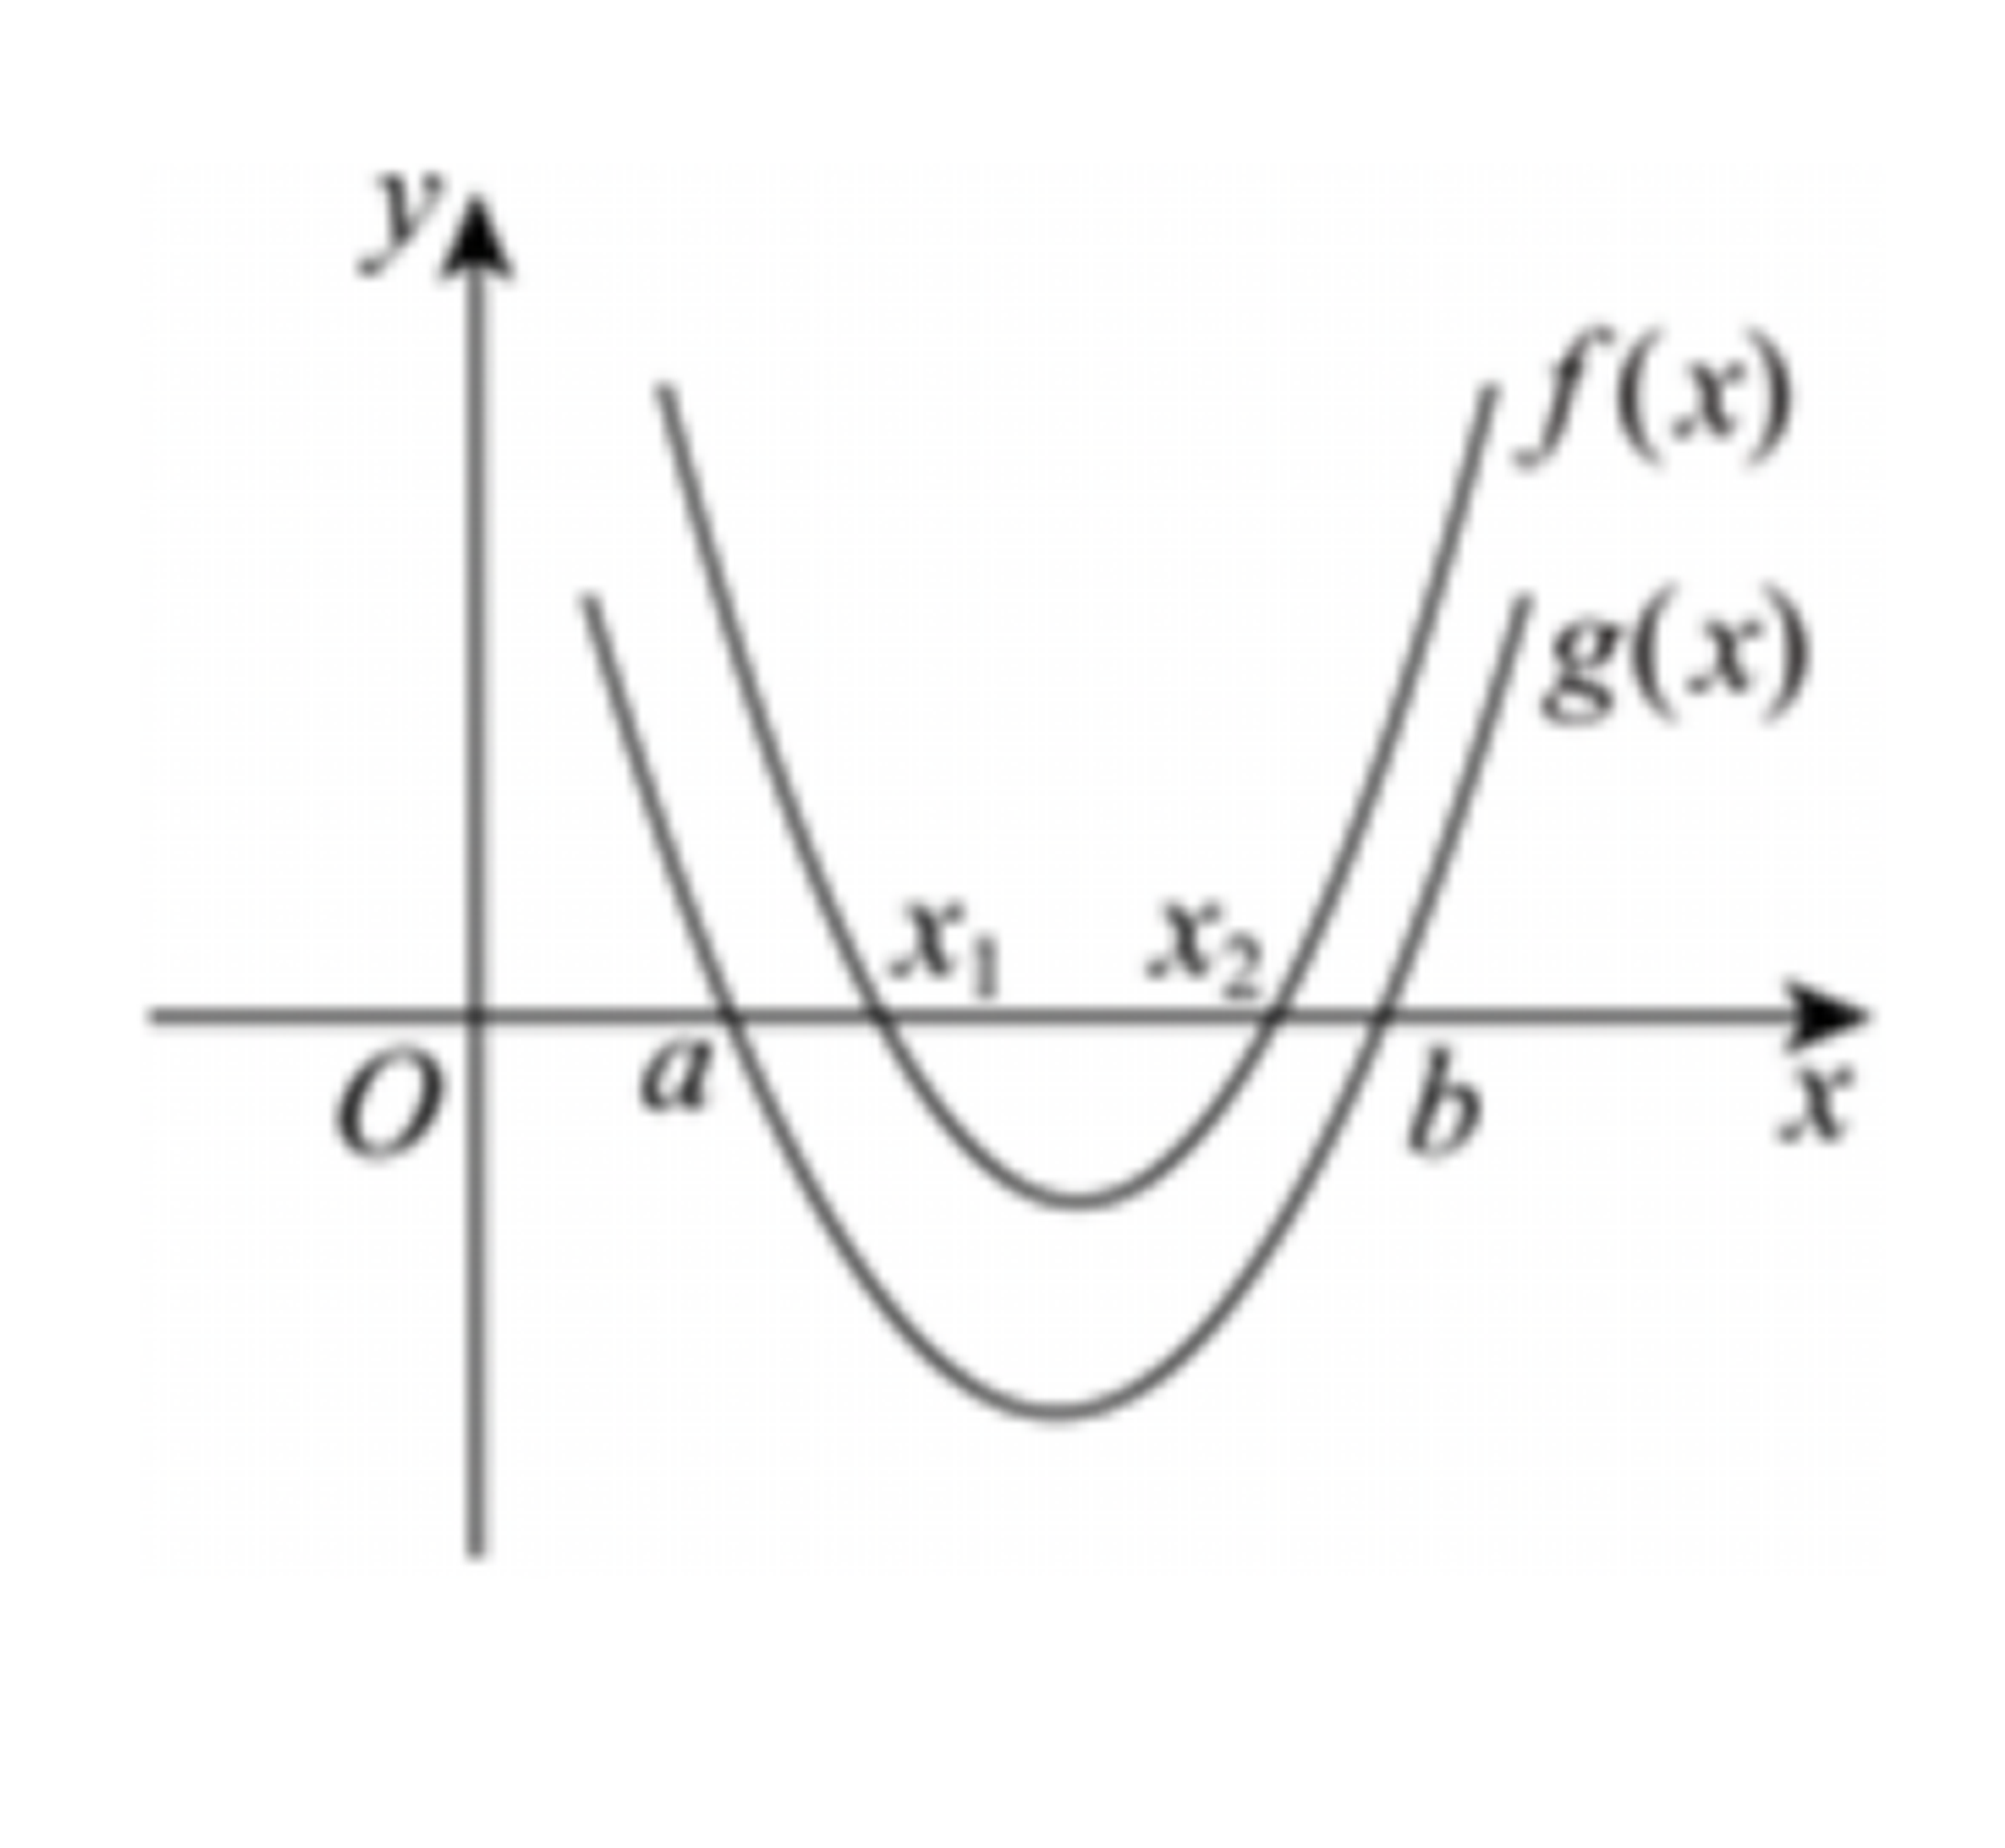
\includegraphics[width=0.30\textwidth]{figures/parabola_f_g_x1x2_h65.png}
\end{center}
\step{由图像得 $a<x_1<x_2<b$，故选 $B$.}
\solend
\fi

\end{enumerate}

\bigsec{三、解答题}

\begin{enumerate}
\setcounter{enumi}{16}

\item 已知 $a>0$，$b>0$，若 $a+b>4$，求证：$\dfrac a{b+2}$ 和 $\dfrac b{a+2}$ 中至少有一个大于 $\dfrac12$.

\ifanswer
\solbegin
\step{假设 $\dfrac a{b+2}\leqslant\dfrac12$，$\dfrac b{a+2}\leqslant\dfrac12$，}
\step{$a>0$，$b>0$，则 $a+2>0$，$b+2>0$，故 $2a\leqslant b+2$，$2b\leqslant a+2$，}
\step{两式相加得 $a+b\leqslant4$，与 $a+b>4$ 矛盾，故 $\dfrac a{b+2}$ 和 $\dfrac b{a+2}$ 中至少有一个大于 $\dfrac12$.}
\solend
\fi

\ansspace[6]

\item 已知集合 $A=\{x\mid-4<x<5\}$，$B=\{x\mid x\leqslant a-6\text{ 或 }x\geqslant a+2\}$.

\begin{enumerate}[label=(\arabic*)]

\item 若 $A\cup B=\R$，求实数 $a$ 的取值范围；

\item 若“$x\in A$”是“$x\in B$”的充分不必要条件，求实数 $a$ 的取值范围.

\end{enumerate}

\ifanswer
\solbegin
\stepm{(1)}{集合 $A=\{x\mid-4<x<5\}$，$B=\{x\mid x\leqslant a-6\text{ 或 }x\geqslant a+2\}$.}
\step{由 $A\cup B=\R$ 得 $\begin{cases}a-6\geqslant-4\\ a+2\leqslant5\end{cases}$，解得 $2\leqslant a\leqslant3$，$a$ 的取值范围为 $[2,3]$；}
\stepm{(2)}{若“$x\in A$”是“$x\in B$”的充分不必要条件，则 $A\subset B$，}
\step{则 $5\leqslant a-6$ 或 $-4\geqslant a+2$，解得 $a\leqslant-6$ 或 $a\geqslant11$.}
\solend
\fi

\ansspace[8]

% 注：原卷题干把命题 $P$ 印作“$\exists3\notin A$”（多一个存在量词），而【解析】两处均作
%     “$3\notin A$”；照录未改，见文件头“原卷笔误/存疑”③。
\item 已知集合 $A=\left\{x\mid\dfrac{x-1}{x-m}<0\right\}$，集合 $B=\left\{x\mid\left|\dfrac{x-1}{x-3}\right|\geqslant1\right\}$，命题 $P$：“$\exists3\notin A$”，命题
$Q$：$A\cap B\neq\varnothing$.

\begin{enumerate}[label=(\arabic*)]

\item 若命题 $P$ 为真命题，求 $m$ 的取值范围；

\item 若命题 $P$ 和命题 $Q$ 至少有一个为假命题，求实数 $m$ 的取值范围.

\end{enumerate}

\ifanswer
\solbegin
\stepm{(1)}{$A=\left\{x\mid\dfrac{x-1}{x-m}<0\right\}=\{x\mid(x-1)(x-m)<0\}$，}
\step{若命题 $P$：“$3\notin A$”为真命题，则 $(3-1)(3-m)\geqslant0$，解得 $m\leqslant3$，}
\step{故实数 $m$ 的取值范围为 $(-\infty,3]$；}
\stepm{(2)}{$B=\left\{x\mid\left|\dfrac{x-1}{x-3}\right|\geqslant1\right\}$，由 $\left|\dfrac{x-1}{x-3}\right|\geqslant1$，得 $\begin{cases}|x-1|\geqslant|x-3|\\ x\neq3\end{cases}$，}
\step{等价于 $\begin{cases}(x-1)^2\geqslant(x-3)^2\\ x\neq3\end{cases}$，解得 $x\geqslant2$ 且 $x\neq3$，所以 $B=[2,3)\cup(3,+\infty)$，}
\step{因为 $A=\{x\mid(x-1)(x-m)<0\}$，}
\step{当 $m=1$ 时，$A=\varnothing$，不满足 $A\cap B\neq\varnothing$，}
\step{当 $m<1$ 时，$A=(m,1)$，不满足 $A\cap B\neq\varnothing$，}
\step{当 $m>1$ 时，$A=(1,m)$，要使 $A\cap B\neq\varnothing$，则 $m>2$，}
\step{则若命题 $Q$：“$A\cap B\neq\varnothing$”为真命题时，实数 $m$ 的取值范围为 $(2,+\infty)$，}
\step{当命题 $P$ 与命题 $Q$ 都是真命题时，则 $\begin{cases}m\leqslant3\\ m>2\end{cases}$，解得 $2<m\leqslant3$，}
\step{则命题 $P$ 和命题 $Q$ 至少有一个为假命题时，得 $m\leqslant2$ 或 $m>3$，}
\step{故实数 $m$ 的取值范围为 $(-\infty,2]\cup(3,+\infty)$.}
\solend
\fi

\ansspace[8]

\item 已知函数 $y=ax^2-(a+2)x+2$，$a\in\R$.

\begin{enumerate}[label=(\arabic*)]

\item $y<3-2x$ 恒成立，求实数 $a$ 的取值范围；

% 注：原卷末句作“求实数 $a$ 的取值”（疑脱“范围”二字），照录未改，
%     见文件头“原卷笔误/存疑”⑤。
\item 若存在 $m>0$ 使关于 $x$ 的方程 $ax^2-(a+2)|x|+2=m+\dfrac1m+1$ 有四个不同的实根，
求实数 $a$ 的取值.

\end{enumerate}

\ifanswer
\solbegin
\stepm{(1)}{由题意得 $ax^2-(a+2)x+2<3-2x$ 恒成立，}
\step{即 $ax^2-ax-1<0$ 恒成立，}
\step{当 $a=0$ 时，$-1<0$ 恒成立，符合题意，}
\step{当 $a\neq0$ 时，则 $\begin{cases}a<0\\ \triangle=a^2+4a<0\end{cases}$，得 $\begin{cases}a<0\\ -4<a<0\end{cases}$，得 $-4<a<0$，}
\step{综上，$a$ 的取值范围为 $(-4,0]$.}
\stepm{(2)}{当 $m>0$ 时，令 $t=m+\dfrac1m+1\geqslant2\sqrt{m\times\dfrac1m}+1=3$，}
\step{当且仅当 $m=1$ 时取等号，}
% 注：题干只给“函数 $y=ax^2-(a+2)x+2$”，全卷未设 $f$，此处 $f(|x|)$ 无定义；
%     照录未改，见文件头“原卷笔误/存疑”④。
\step{则关于 $x$ 的方程 $f(|x|)=t$ 可化为 $a|x|^2-(a+2)|x|+2-t=0$，}
\step{关于 $x$ 的方程为 $a|x|^2-(a+2)|x|+2-t=0$ 有四个不等的实数根，}
\step{即 $ax^2-(a+2)x+2-t=0$，有两个不同的实数正根，}
\step{则 $\begin{cases}\triangle=(a+2)^2-4a(2-t)>0\\ \dfrac{a+2}a>0\\ \dfrac{2-t}a>0\end{cases}$，解得 $a<-2$，}
\step{由（1）得存在 $t\in[3,+\infty)$ 使得不等式 $4at+(a+2)^2-8a>0$ 成立，}
\step{故 $4a\times3+(a+2)^2-8a>0$，即 $a^2+8a+4>0$，}
\step{解得 $a<-4-2\sqrt3$ 或 $a>-4+2\sqrt3$，}
\step{综上，$a<-4-2\sqrt3$，所以 $a$ 的取值范围为 $(-\infty,-4-2\sqrt3)$.}
\solend
\fi

\ansspace[8]

\item 若集合 $A=B_1\cup B_2\cup\cdots\cup B_n$，其中 $B_1$、$B_2$、$\cdots$、$B_n$ 为非空集合，
$B_i\cap B_j=\varnothing$($1\leqslant i<j\leqslant n$)，则称集合 $\{B_1,B_2,\cdots,B_n\}$ 为集合 $A$ 的一个 $n$ 划分.

\begin{enumerate}[label=(\arabic*)]

\item 写出集合 $A=\{1,2,3\}$ 的所有不同的 2 划分；

\item 设 $\{B_1,B_2\}$ 为有理数集 $\Q$ 的一个 2 划分，且满足对任意 $x\in B_1$，任意 $y\in B_2$，都有
$x<y$，判断命题“$B_1$ 中的元素存在最大值，$B_2$ 中的元素存在最小值.”的真假，并说明
理由.

\item 设集合 $A=\{1,2,3,\cdots,16\}$，对于集合 $A$ 的任意一个 3 划分 $\{B_1,B_2,B_3\}$，判断是否存
在 $i\in\{1,2,3\}$，存在 $a$、$b\in B_i$，使得 $b-a\in B_i$ 成立，并说明理由.

\end{enumerate}

\ifanswer
\solbegin
% 注：原卷三个“2 划分”本有外层花括号（$\{\{1,2\},\{3\}\}$ 等），首轮误脱；
%     第二轮复核照原卷补回（原卷原样 / 本稿原错处：原脱外层花括号）。
\stepm{(1)}{集合 $A=\{1,2,3\}$ 的所有不同的 2 划分为 $\{\{1,2\},\{3\}\}$、$\{\{1,3\},\{2\}\}$、}
\step{$\{\{2,3\},\{1\}\}$.}
\stepm{(2)}{该命题为假命题，理由如下：}
\step{假设命题为真，则不妨设 $B_1$ 中元素的最大值为 $s$，$B_2$ 中元素的最小值为 $t$，}
\step{由题意得 $s<t$，所以 $s<\dfrac{s+t}2<t$，}
\step{因为 $s$ 为 $B_1$ 中元素的最大值，所以 $\dfrac{s+t}2\notin B_1$，}
\step{因为 $t$ 为 $B_2$ 中元素的最小值，所以 $\dfrac{s+t}2\notin B_2$，}
\step{因为 $B_1\cup B_2=\Q$，所以 $\dfrac{s+t}2\notin\Q$，}
\step{这与 $\dfrac{s+t}2\in\Q$ 矛盾，所以假设不成立，即命题不可能成立；}
\stepm{(3)}{由于集合 $A$ 中有 16 个元素，}
\step{所以 $B_1$、$B_2$、$B_3$ 中至少有一个集合至少包含 6 个元素，}
\step{不妨设 $B_1$ 中至少包含 6 个元素，}
\step{设 $b_1$、$b_2$、$b_3$、$b_4$、$b_5$、$b_6\in B_1$，且 $b_1<b_2<b_3<b_4<b_5<b_6$，}
\step{假设对任意 $i\in\{1,2,3\}$，对任意 $a$、$b\in B_i$，都有 $b-a\notin B_i$，}
\step{那么 $b_6-b_1$、$b_6-b_2$、$b_6-b_3$、$b_6-b_4$、$b_6-b_5\notin B_1$，}
\step{又因为 $b_6-b_1$、$b_6-b_2$、$b_6-b_3$、$b_6-b_4$、$b_6-b_5\in A$，}
\step{所以 $b_6-b_1$、$b_6-b_2$、$b_6-b_3$、$b_6-b_4$、$b_6-b_5\in B_2\cup B_3$，}
\step{则 $B_2$、$B_3$ 中必有一个集合}
\step{至少包含 $b_6-b_1$、$b_6-b_2$、$b_6-b_3$、$b_6-b_4$、$b_6-b_5$ 中的 3 个元素，}
\step{不妨设这 3 个元素为 $a_1$、$a_2$、$a_3\in B_2$，$a_1<a_2<a_3$，}
\step{由假设得 $a_3-a_1$、$a_3-a_2$、$a_2-a_1\notin B_2$，}
\step{对任意 $i$、$j$($1\leqslant j<i\leqslant3$)，存在 $m$、$n$($1\leqslant m<n\leqslant5$)，}
\step{都有 $a_i-a_j=b_6-b_m-b_6+b_n=b_n-b_m\notin B_1$，}
\step{又因为 $a_3-a_1$、$a_3-a_2$、$a_2-a_1\in B_3$，而 $a_3-a_1-(a_3-a_2)=a_2-a_1$，}
\step{与假设矛盾，所以假设不成立，}
\step{即存在 $i\in\{1,2,3\}$，存在 $a$、$b\in B_i$，使得 $b-a\in B_i$.}
\solend
\fi

\ansspace*[10]

\end{enumerate}

\end{document}
"
%
% 原始材料：微信公众号“魔都数学加油站”文章，作者破晓，连载“27学年高一65”；
% 原文标题“27学年高一65——2026-2027年上海市大同中学高一上10月月考”；
% 原文链接：https://mp.weixin.qq.com/s/h9ctuk-ByE1Vfg2Rx2C6bw。
% 页面标注发布时间 2026-10-17 21:58（上海）。
% 本次转录只据 `原图/高一65_大同中学_10月月考/` 的 11 张 PNG 逐页读图。
% 正文为 11 张 PNG 页（`01..11.png`）：
% 第 06、11 页 2560×3620，第 01、02、03、04、05、07、08、09、10 页 4762×6735
% （**同一篇各页分辨率不同**），均按页序读取。11 页全为试卷正文页（卷首标题在第 1 页页顶，
% 卷末解答题第 21 题解析止于第 11 页），无封面页、目录页、二维码或宣传页。
% 粉色斜排“魔都数学加油站”为卷面水印，与公众号页脚一并未录入。
%
% 卷首标题：照卷面印作“2026--2027 年大同中学高一上 10 月月考”，年份区间按全稿惯例排 en dash。
% 原卷只有一行标题、无副标题。
%
% 篇幅与题号：原卷自第 3 题起编号（第 1、2 题不在本卷内）。填空题 3—12（10 题）、
% 选择题 13—16（4 题）、解答题 17—21（5 题），共 19 题。本稿沿用原节与原题号，
% 只改排为全稿统一的大节样式（原卷小节标题为“一、填空题”“二、选择题”“三、解答题”）。
%
% 讲评版：原卷每题下直接印【答案】或【解析】。**只印【答案】的 4 题**（第 3、4、7、10 题），
% 本稿只给 \ans{}；其余 15 题都印【解析】（按全稿口径这类题不另提 \ans{}——第 12、13、14、
% 15、16 题的结论写在解析末句（“故选 B”“综上，n 的最大值为 14”等），亦照录在解析内）。
% 全卷无“答案印在题干括号内”的题（第 13—16 题的选择题括号内均空白）。
%
% 副标题：原卷未印副标题。本稿按“知识模块”口径标作“集合与常用逻辑用语、不等式”：
% 19 题中集合与常用逻辑用语 10 题（第 3、4、6、8、12、14、15、18、19、21 题），
% 不等式 9 题（含等式恒等、不等式性质、二次不等式、恒成立、基本不等式、不等式的证明：
% 第 5、7、9、10、11、13、16、17、20 题），两类均超过三分之一，故并标。口径同 高一63。
%
% 与原卷的排版差异：
%   ① 原卷每题下直接印【答案】/【解析】，本稿按全稿惯例将答案与解析置于答案版，试卷版保持干净；
%   ② 原卷未印副标题，本稿按“知识模块”口径补出；
%   ③ 原卷填空横线约四个字宽，本稿按全稿惯例统一排 \blankline[4.4em]；
%   ④ 原卷数集记号全为斜体：实数集作 $R$（第 6 题两处、第 8 题两处、第 15 题解析、第 18 题、
%      第 20 题题干），自然数集作 $N$（第 12 题题干“$n\in N,n\geqslant1$”），有理数集作 $Q$
%      （第 21 题 (2) 题干与解析共 4 处），本稿按全稿惯例统一改用 $\R$、$\N$、$\Q$
%      （同 高一63 排版差异④：记号归一）；空集记号原卷作 $\varnothing$，照录；
%   ⑤ 原卷用描述法时竖线排细竖“$|$”（如 $\{x|0<x<3\}$、$\{x|(x-1)(x-m)<0\}$），
%      本稿按全稿惯例排 \mid；
%   ⑥ 原卷判别式印作“$\triangle$”（第 8、14 题解析各 1 处、第 20 题解析 2 处，共 4 处），
%      本稿照录用 \triangle（同 高一39 成例），未改作 \Delta；
%   ⑦ 第 18—21 题的子问原卷各自另起一行、以“（1）”“（2）”标号，本稿按全稿惯例用
%      enumerate 的 (1)(2)(3)；解析中的子问标号一律用 \stepm{(1)}{…}；
%      第 18—21 题解析（原文以“（1）”“（2）”“（3）”冠于解析首句）同此；
%   ⑧ 选择题的作答括号原卷排半角“(　　)”（第 13—16 题括号内均空白），
%      本稿按全稿惯例排 \mbox{（\quad）}；选项字母后的句点照原卷排“A.”“B.”；
%   ⑨ 每道解答题原卷未留作答空白，本稿按全稿惯例加 \ansspace（末题用 \ansspace*）；
%   ⑩ 原卷在数学式内多处用半角逗号（如 $\{x|0<x<3\},B=\{x|x>2\}$、$m\in I_{14},k\in I_{14}$），
%      均照录未强改；句末句点按全稿惯例排西文句点。
%
% 原卷笔误/存疑（均照录未改，正文对应处另有 % 注）：
%   ① 第 13 题题干“下列不等式中一定成立是（　　）”脱一个“的”（当作“一定成立的是”），
%      8 倍放大确认非水印遮挡，本稿照录；
%   ② 第 15 题【解析】末段把题干条件“$x\geqslant10$”写成“$x\geqslant1$”
%      （“所以 $x+2+\frac{16}{x+2}(x\geqslant1)$ 的最小值不为 8”），与同段前面“令 $t=x+2$，
%      则 $t\geqslant12$”不合，本稿照录；
%   ③ 第 19 题题干把命题 $P$ 印作“$\exists3\notin A$”（多一个存在量词），而【解析】两处
%      均作“$3\notin A$”，前后记号不一，本稿照录；
%   ④ 第 20 题【解析】(2) 出现 $f(|x|)$，但题干只给“函数 $y=ax^2-(a+2)x+2$”、全卷未设 $f$，
%      本稿照录；
%   ⑤ 第 20 题 (2) 题干末句作“求实数 $a$ 的取值”（疑脱“范围”二字），本稿照录；
%   ⑥ 第 12 题【解析】第 18 步“它与 $P_n$ 中的任何其他数之和都不是整数”，该段所论为 $P_{14}$
%      （前后均作 $P_{14}$），此处 $P_n$ 疑当作 $P_{14}$，本稿照录。
%
% 第二轮复核（2026-10-18）订正「本稿抄错原卷」一处：
%   第 21 题 (1)【解析】原卷本作“$\{\{1,2\},\{3\}\}$、$\{\{1,3\},\{2\}\}$、$\{\{2,3\},\{1\}\}$”，
%   有外层花括号；首轮误脱外层花括号，并曾在文件头误记为“原卷未加外层花括号”（原第 ⑦ 条，
%   已撤销）。本次照原卷补回，正文对应处另有 % 注。
%
% 插图：第 16 题【解析】内有 1 幅图（两条开口向上的抛物线 $f(x)$、$g(x)$ 与 $x$ 轴交点
% 标 $a$、$x_1$、$x_2$、$b$，纵轴标 $y$、原点 $O$），解析第三行“画出函数 $g(x)$ 与函数 $f(x)$
% 的图像，如图所示”即指此图；取原卷截图（06.png，2560×3620）右半幅，4× LANCZOS 放大，
% 存 figures/parabola_f_g_x1x2_h65.png。该图在【解析】内，仅答案版出。
%
\documentclass[a4paper,11pt]{article}
\usepackage{common}

\begin{document}

\examtitlest[3]{2026--2027 年大同中学高一上 10 月月考}{集合与常用逻辑用语、不等式}

\bigsec{一、填空题}

\begin{enumerate}
\setcounter{enumi}{2}

\item 已知集合 $A=\{x\mid0<x<3\}$,$B=\{x\mid x>2\}$，则集合 $A\cup B=$\blankline[4.4em].

\ifanswer
\ans{$(0,+\infty)$}
\fi

\item “$x>1$ 或 $y>1$”的否定形式是\blankline[4.4em].

\ifanswer
\ans{$x\leqslant1$ 且 $y\leqslant1$}
\fi

\item 已知等式 $2x^2+3x+4=a(2x+1)(x+1)+b$ 恒成立，则常数 $a-b=$\blankline[4.4em].

\ifanswer
\solbegin
\step{因为等式 $2x^2+3x+4=a(2x+1)(x+1)+b$ 恒成立，}
\step{所以 $a(2x+1)(x+1)+b=2ax^2+3ax+a+b=2x^2+3x+4$，}
\step{所以 $\begin{cases}2a=2\\ 3a=3\\ a+b=4\end{cases}$，解得 $\begin{cases}a=1\\ b=3\end{cases}$，所以 $a-b=-2$.}
\solend
\fi

\item 全集为 $U=\R$，$A=\{x\mid|x|\geqslant2\}$，$B=\{y\mid y=x^2+1,x\in\R\}$，则 $A\cup\bar B=$\blankline[4.4em].

\ifanswer
\solbegin
\step{由题意得集合 $A=\{x\mid x\geqslant2\text{ 或 }x\leqslant-2\}$，}
\step{因为 $x^2+1\geqslant1$，所以集合 $B=\{x\mid x\geqslant1\}$，所以 $\bar B=\{x\mid x<1\}$，}
\step{则 $A\cup\bar B=\{x\mid x\geqslant2\text{ 或 }x<1\}$.}
\solend
\fi

\item 已知 $|x+3|+|x-5|=8$，则实数 $x$ 的取值范围为\blankline[4.4em].

\ifanswer
\ans{$[-3,5]$}
\fi

\item 已知集合 $A=\{x\in\R\mid ax^2+2x+1=0,a\in\R\}$ 只有一个元素，则 $a$ 的值为\blankline[4.4em].

\ifanswer
\solbegin
\step{当 $a=0$ 时，$A=\left\{-\dfrac12\right\}$；}
\step{当 $a\neq0$ 时，若集合 $A$ 只有一个元素，由 $\triangle=4-4a=0$ 得 $a=1$.}
\step{综上，当 $a=0$ 或 $a=1$ 时，集合 $A$ 只有一个元素.}
\solend
\fi

\item 已知不等式 $-x^2+bx+c>0$ 的解集为 $(3,4)$，则不等式 $cx^2+bx-1<0$ 的解集为\blankline[4.4em].

\ifanswer
\solbegin
\step{由题意得 3，4 是方程 $-x^2+bx+c=0$ 的两个实数根，}
\step{所以 $\begin{cases}3+4=b\\ 3\times4=-c\end{cases}$，得 $b=7$，$c=-12$，}
\step{则不等式 $cx^2+bx-1<0$，即为 $-12x^2+7x-1<0$，即 $12x^2-7x+1>0$，}
\step{化简得 $(3x-1)(4x-1)>0$，解得 $x<\dfrac14$ 或 $x>\dfrac13$，}
\step{即不等式 $cx^2+bx-1<0$ 的解集为 $\left(-\infty,\dfrac14\right)\cup\left(\dfrac13,+\infty\right)$.}
\solend
\fi

\item 对于区间 $(m,n)$，我们将 $n-m$ 的值称为该区间的长度. 若关于 $x$ 的不等式
$x^2+ax+a<0$ 有解，且解集的区间长度不超过 $2\sqrt3$，则实数 $a$ 的取值范围是\blankline[4.4em].

\ifanswer
\ans{$[-2,0)\cup(4,6]$}
\fi

\item 当 $x>0$ 时，关于 $x$ 的不等式 $(ax-1)(x^2+bx-4)\geqslant0$ 恒成立，则 $b+\dfrac2a$ 的最小值
为\blankline[4.4em].

\ifanswer
\solbegin
\step{由题意 $a\neq0$；}
\step{若 $a<0$，则 $x>0$ 时 $ax-1<0$ 恒成立，需 $x^2+bx-4\leqslant0$ 对一切 $x>0$ 成立，}
\step{而 $y=x^2+bx-4$ 的图象开口向上，当 $x$ 充分大时必为正值，矛盾，故 $a>0$.}
\step{当 $a>0$ 时，$ax-1=a\left(x-\dfrac1a\right)$，故原条件化为 $\left(x-\dfrac1a\right)(x^2+bx-4)\geqslant0$：}
\step{若 $0<x<\dfrac1a$，则 $x-\dfrac1a<0$，需 $x^2+bx-4\leqslant0$；}
\step{若 $x>\dfrac1a$，则 $x-\dfrac1a>0$，需 $x^2+bx-4\geqslant0$；}
\step{由 $y=x^2+bx-4$ 的连续性知 $x=\dfrac1a$ 是它的零点，}
\step{即 $\dfrac1{a^2}+\dfrac ba-4=0$，得 $b=4a-\dfrac1a$；}
\step{此时 $x^2+bx-4=x^2+\left(4a-\dfrac1a\right)x-4=(x+4a)\left(x-\dfrac1a\right)$，}
\step{由 $a>0$、$x>0$ 得 $x+4a>0$，}
\step{其符号与 $x-\dfrac1a$ 一致，故能与 $ax-1$ 同号，原不等式确在 $x>0$ 上恒成立.}
\step{于是 $b+\dfrac2a=4a-\dfrac1a+\dfrac2a=4a+\dfrac1a\geqslant2\sqrt{4a\cdot\dfrac1a}=4$，}
\step{当且仅当 $a=\dfrac12$ 时取等号，故最小值为 4.}
\solend
\fi

\item 设集合 $I_n=\{1,2,\cdots,n\}$，$n\in\N$，$n\geqslant1$，集合 $P_n=\left\{\dfrac m{\sqrt k}\mid m\in I_n,k\in I_n\right\}$，若 $P_n$ 的子集 $A$
中任意两个元素之和不是整数的平方，则称 $A$ 为“人文集”. 那么使 $P_n$ 能分成两个交集为空
集的“人文集”的并集，且这两个人文集的并集恰为 $P_n$ 时，$n$ 的最大值是\blankline[4.4em].

\ifanswer
\solbegin
\step{先证当 $n\geqslant15$ 时，$P_n$ 不能分成两个不相交的人文集的并集.}
\step{假设当 $n\geqslant15$ 时，$P_n$ 可以分成两个不相交的人文集的并集，}
\step{设 $A$ 和 $B$ 为两个不相交的人文集，使 $A\cup B=P_n\supseteq I_n$.}
\step{不妨设 $1\in A$，则由于 $1+3=2^2$，所以 $3\notin A$，即 $3\in B$.}
\step{同理可得，$6\in A$，$10\in B$. 又推出 $15\in A$，}
\step{但 $1+15=4^2$，这与 $A$ 为人文集相矛盾.}
\step{再证 $P_{14}$ 满足要求. 当 $k=1$ 时，$P_{14}=\left\{\dfrac m{\sqrt k}\mid m\in I_{14},k\in I_{14}\right\}$，}
\step{可以分成 2 个人文集的并集.}
\step{事实上，只要取 $A_1=\{1,2,4,6,9,11,13\}$，$B_1=\{3,5,7,8,10,12,14\}$，}
\step{则 $A_1$ 和 $B_1$ 都是人文集，且 $A_1\cup B_1=P_{14}$.}
\step{当 $k=4$ 时，集合 $\left\{\dfrac m{\sqrt k}\mid m\in I_{14}\right\}$ 中，除整数外，}
\step{剩下的数组成集合 $\left\{\dfrac12,\dfrac32,\dfrac52,\cdots,\dfrac{13}2\right\}$，}
\step{可以分为下列 2 个人文集的并：$A_2=\left\{\dfrac12,\dfrac52,\dfrac92,\dfrac{11}2\right\}$，$B_2=\left\{\dfrac32,\dfrac72,\dfrac{13}2\right\}$.}
\step{当 $k=9$ 时，集合 $\left\{\dfrac m{\sqrt k}\mid m\in I_{14}\right\}$ 中，除整数外，}
\step{剩下的数组成集合 $\left\{\dfrac13,\dfrac23,\dfrac43,\dfrac53,\cdots,\dfrac{13}3,\dfrac{14}3\right\}$，}
\step{可以分为下列 2 个人文集的并：$A_3=\left\{\dfrac13,\dfrac43,\dfrac53,\dfrac{10}3,\dfrac{13}3\right\}$，$B_3=\left\{\dfrac23,\dfrac73,\dfrac83,\dfrac{11}3,\dfrac{14}3\right\}$.}
\step{最后，集合 $C=\left\{\dfrac m{\sqrt k}\mid m\in I_{14},k\in I_{14},k\neq1,4,9\right\}$ 中的数的分母都是无理数，}
% 注：本行原卷作“$P_n$”，而该段所论为 $P_{14}$（前后均作 $P_{14}$），疑当作 $P_{14}$；
%     照录未改，见文件头“原卷笔误/存疑”⑥。
\step{它与 $P_n$ 中的任何其他数之和都不是整数，}
\step{因此，令 $A=A_1\cup A_2\cup A_3\cup C$，$B=B_1\cup B_2\cup B_3$，}
\step{则 $A$ 和 $B$ 是不相交的人文集，且 $A\cup B=P_{14}$.}
\step{综上，$n$ 的最大值为 14.}
\solend
\fi

\end{enumerate}

\bigsec{二、选择题}

\begin{enumerate}
\setcounter{enumi}{12}

% 注：原卷题干“下列不等式中一定成立是”脱一个“的”（当作“一定成立的是”），
%     照录未改，见文件头“原卷笔误/存疑”①。
\item 已知 $a>b$，下列不等式中一定成立是\mbox{（\quad）}

\keepwithprev
A. $a^2>b^2$\qquad B. $ac^2>bc^2$\qquad C. $\dfrac1a<\dfrac1b$\qquad D. $a+3>b-4$

\ifanswer
\solbegin
\step{对于 $A$，当 $a=-2$，$b=-4$ 时，不等式不成立，故 $A$ 错误；}
\step{对于 $B$，当 $c=0$ 时，不等式不成立，故 $B$ 错误；}
\step{对于 $C$，当 $a=2$，$b=-4$ 时，不等式不成立，故 $C$ 错误；}
\step{对于 $D$，因为 $a>b$，$3>-4$，必有 $a+3>b-4$ 成立，故 $D$ 正确.}
\step{故选 $D$.}
\solend
\fi

\item 已知 $a$ 为实数，那么“$|a|\leqslant2$”是“方程 $x^2+ax+1=0$ 没有实数解”的\mbox{（\quad）}

\keepwithprev
A. 充分而不必要条件\qquad B. 必要而不充分条件

C. 充要条件\qquad D. 既不充分也不必要条件

\ifanswer
\solbegin
\step{由方程 $x^2+ax+1=0$ 没有实数解，得 $\triangle=a^2-4<0$，则 $|a|<2$，}
\step{由 $|a|<2$ 得 $|a|\leqslant2$，反之不成立，}
\step{所以“$|a|\leqslant2$”是“方程 $x^2+ax+1=0$ 没有实数解”的必要而不充分条件.}
\step{故选 $B$.}
\solend
\fi

\item 下列命题为真命题的是\mbox{（\quad）}

\keepwithprev
A. $a>b>0$，当 $m>0$ 时，$\dfrac{a+m}{b+m}>\dfrac ab$

B. 集合 $A=\{x\mid y=x^2+1\}$ 与集合 $B=\{y\mid y=x^2+1\}$ 是相同的集合

C. 若 $b<a<0$，$m<0$，则 $\dfrac ma>\dfrac mb$

D. $x+2+\dfrac{16}{x+2}(x\geqslant10)$ 最小值为 8

\ifanswer
\solbegin
\step{对于 $A$，$\dfrac{a+m}{b+m}-\dfrac ab=\dfrac{b(a+m)-a(b+m)}{b(b+m)}=\dfrac{m(b-a)}{b(b+m)}$，}
\step{因为 $a>b>0$，$m>0$，所以 $b(b+m)>0$，$m(b-a)<0$，}
\step{所以 $\dfrac{a+m}{b+m}-\dfrac ab=\dfrac{m(b-a)}{b(b+m)}<0$，}
\step{即 $a>b>0$，当 $m>0$ 时，$\dfrac{a+m}{b+m}<\dfrac ab$，故 $A$ 错误；}
\step{对于 $B$，集合 $A=\{x\mid y=x^2+1\}=\R$，集合 $B=\{y\mid y=x^2+1\}=\{y\mid y\geqslant1\}$，}
\step{所以 $A\neq B$，故 $B$ 错误；}
\step{对于 $C$，$\dfrac ma-\dfrac mb=\dfrac{m(b-a)}{ab}$，}
\step{因为 $b<a<0$，$m<0$，所以 $ab>0$，$m(b-a)>0$，}
\step{所以 $\dfrac ma-\dfrac mb=\dfrac{m(b-a)}{ab}>0$，即 $\dfrac ma>\dfrac mb$，故 $C$ 正确；}
\step{对于 $D$，令 $t=x+2$，则 $t\geqslant12$，表达式变为 $t+\dfrac{16}t$，}
\step{$t+\dfrac{16}t\geqslant2\sqrt{t\cdot\dfrac{16}t}=8$，当且仅当 $t=4$ 时取等号，即等号不成立，}
% 注：原卷本行把题干条件“$x\geqslant10$”写成“$x\geqslant1$”，与同段“$t\geqslant12$”不合；
%     照录未改，见文件头“原卷笔误/存疑”②。
\step{所以 $x+2+\dfrac{16}{x+2}(x\geqslant1)$ 的最小值不为 8，故 $D$ 错误.}
\step{故选 $C$.}
\solend
\fi

\item 已知实数 $a<b$，关于 $x$ 的不等式 $x^2-(a+b)x+ab+\dfrac12<0$ 的解集为 $(x_1,x_2)$，则实数 $a$、
$b$、$x_1$、$x_2$ 从小到大的排列是\mbox{（\quad）}

\keepwithprev
A. $x_1<a<b<x_2$\qquad B. $a<x_1<x_2<b$\qquad C. $a<x_1<b<x_2$\qquad D. $x_1<a<x_2<b$

\ifanswer
\solbegin
\step{不等式 $x^2-(a+b)x+ab+\dfrac12<0$ 可化为 $(x-a)(x-b)+\dfrac12<0$，}
\step{设 $g(x)=(x-a)(x-b)$，$f(x)=g(x)+\dfrac12$，}
\step{画出函数 $g(x)$ 与函数 $f(x)$ 的图像，如图所示，}
% 图在【解析】内（仅答案版出），取原卷截图（06.png，2560×3620）右半幅，4× LANCZOS 放大。
\begin{center}
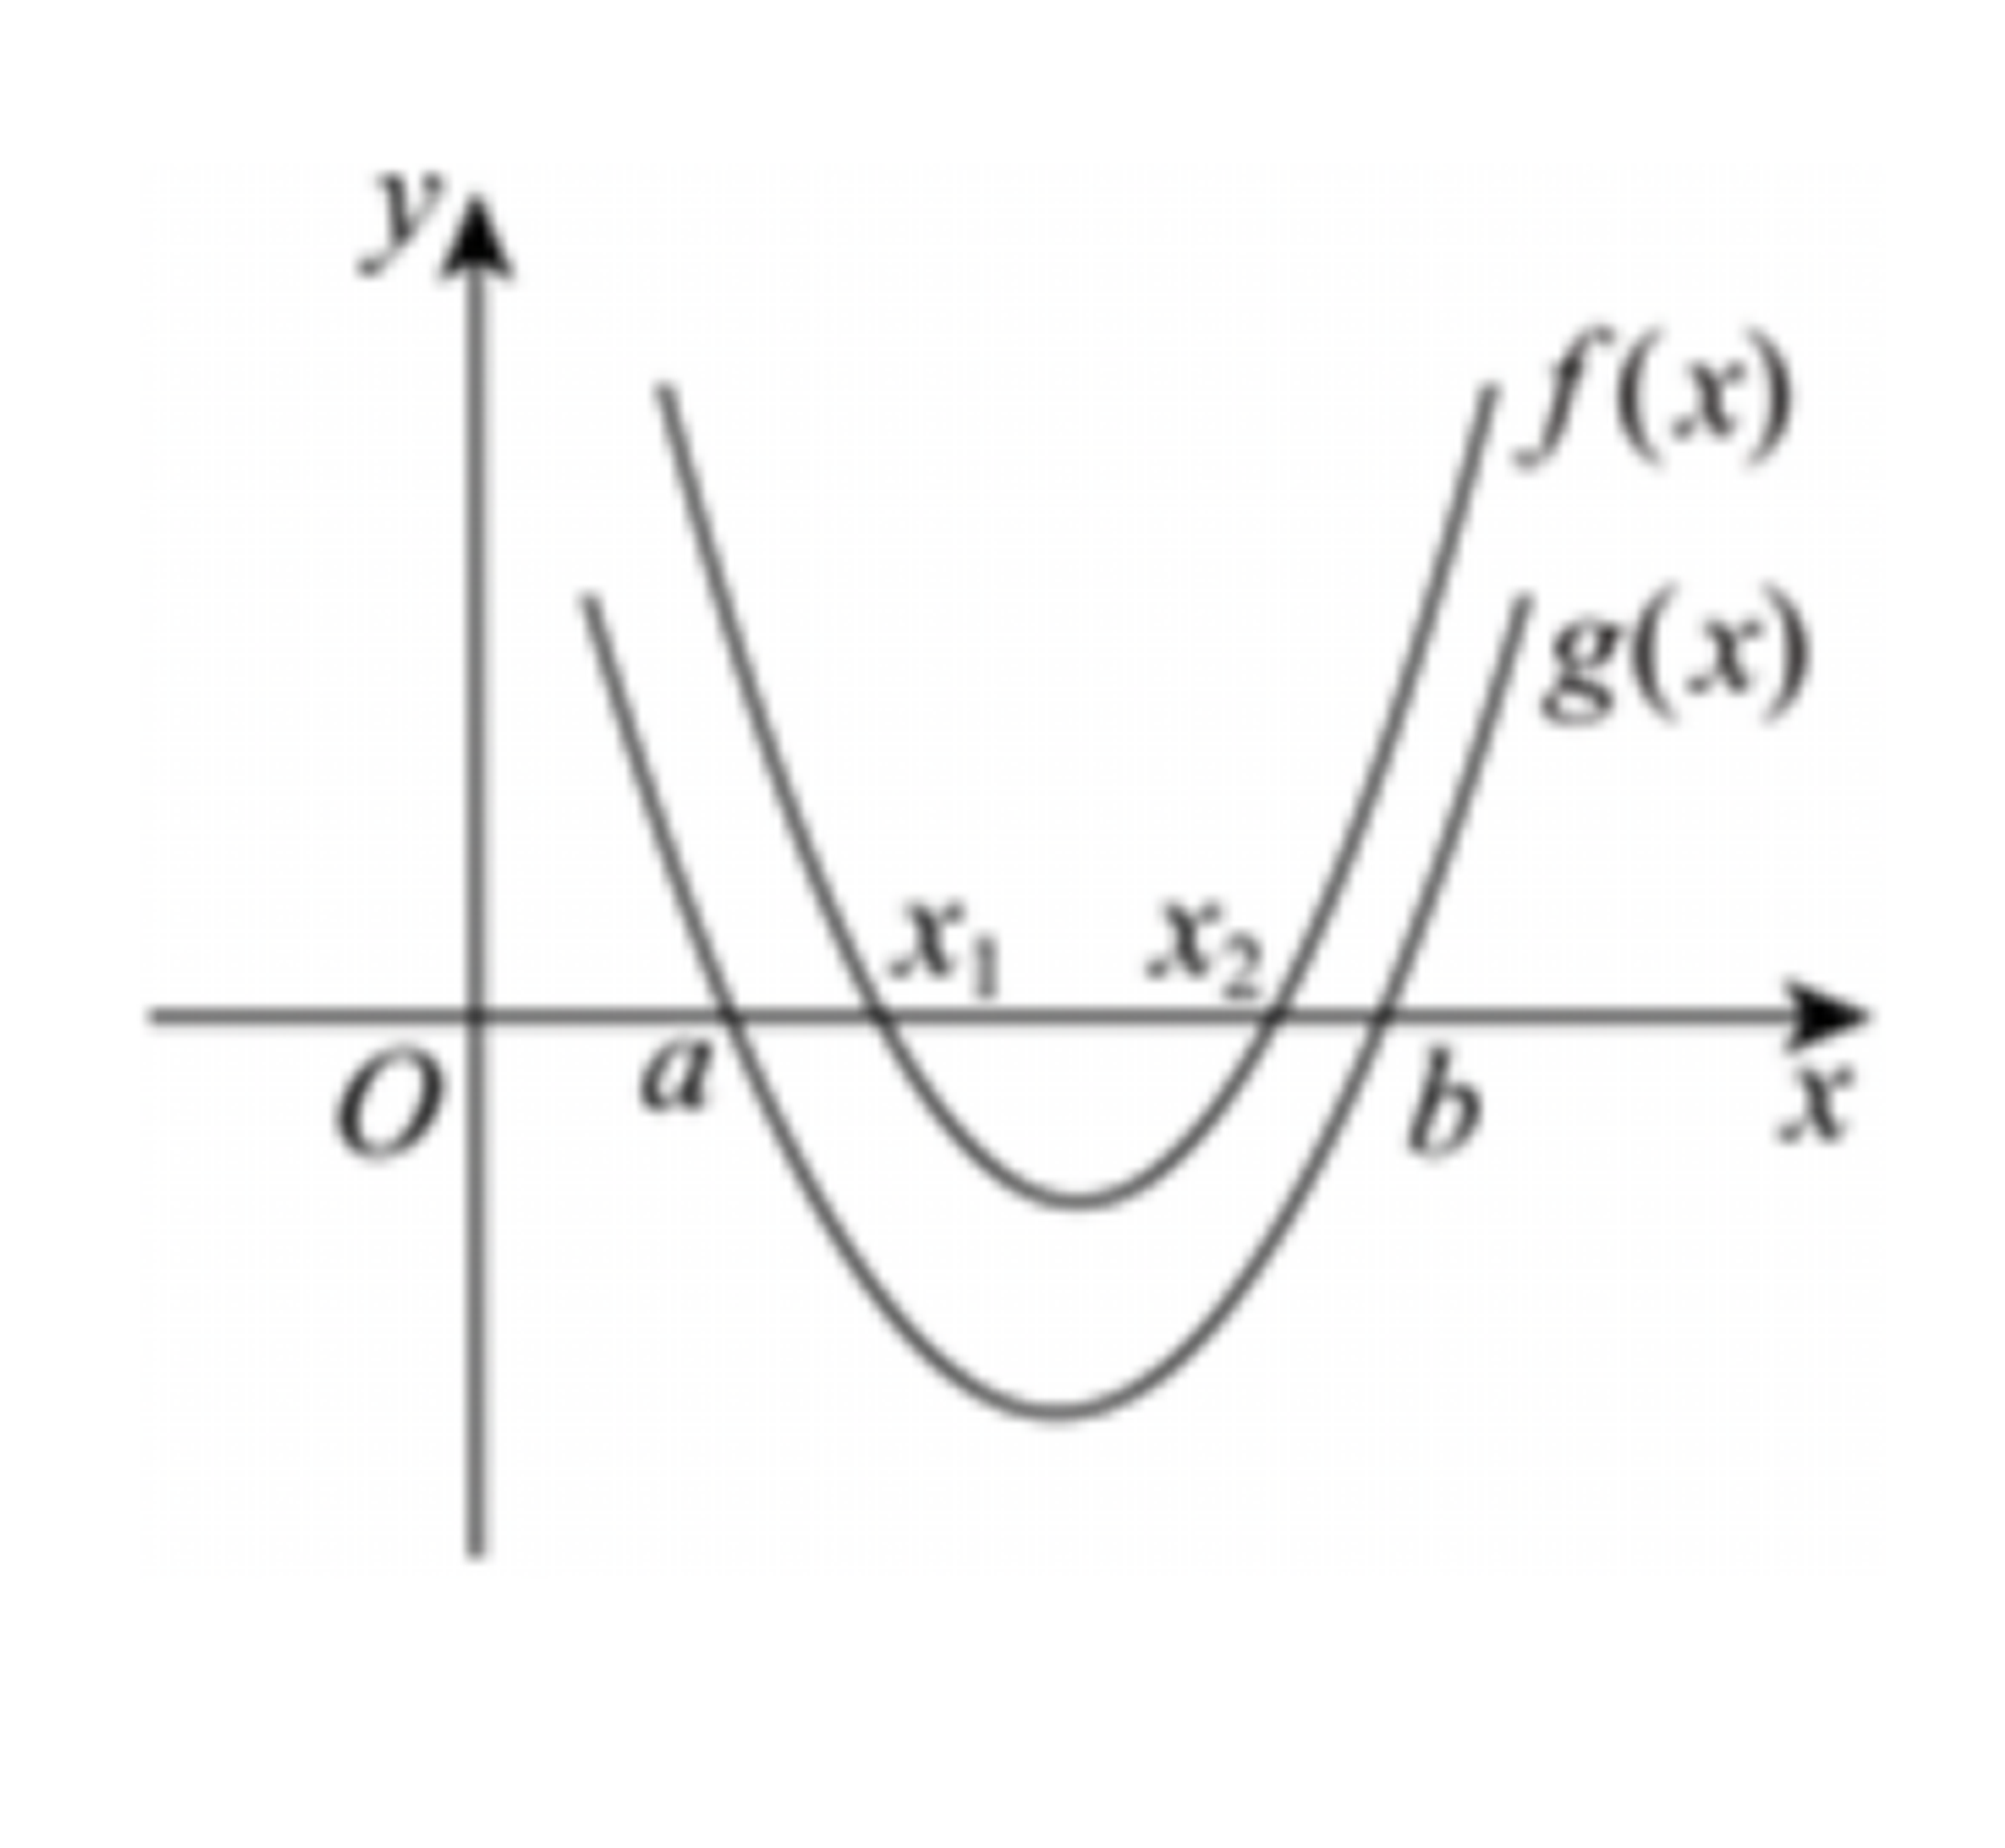
\includegraphics[width=0.30\textwidth]{figures/parabola_f_g_x1x2_h65.png}
\end{center}
\step{由图像得 $a<x_1<x_2<b$，故选 $B$.}
\solend
\fi

\end{enumerate}

\bigsec{三、解答题}

\begin{enumerate}
\setcounter{enumi}{16}

\item 已知 $a>0$，$b>0$，若 $a+b>4$，求证：$\dfrac a{b+2}$ 和 $\dfrac b{a+2}$ 中至少有一个大于 $\dfrac12$.

\ifanswer
\solbegin
\step{假设 $\dfrac a{b+2}\leqslant\dfrac12$，$\dfrac b{a+2}\leqslant\dfrac12$，}
\step{$a>0$，$b>0$，则 $a+2>0$，$b+2>0$，故 $2a\leqslant b+2$，$2b\leqslant a+2$，}
\step{两式相加得 $a+b\leqslant4$，与 $a+b>4$ 矛盾，故 $\dfrac a{b+2}$ 和 $\dfrac b{a+2}$ 中至少有一个大于 $\dfrac12$.}
\solend
\fi

\ansspace[6]

\item 已知集合 $A=\{x\mid-4<x<5\}$，$B=\{x\mid x\leqslant a-6\text{ 或 }x\geqslant a+2\}$.

\begin{enumerate}[label=(\arabic*)]

\item 若 $A\cup B=\R$，求实数 $a$ 的取值范围；

\item 若“$x\in A$”是“$x\in B$”的充分不必要条件，求实数 $a$ 的取值范围.

\end{enumerate}

\ifanswer
\solbegin
\stepm{(1)}{集合 $A=\{x\mid-4<x<5\}$，$B=\{x\mid x\leqslant a-6\text{ 或 }x\geqslant a+2\}$.}
\step{由 $A\cup B=\R$ 得 $\begin{cases}a-6\geqslant-4\\ a+2\leqslant5\end{cases}$，解得 $2\leqslant a\leqslant3$，$a$ 的取值范围为 $[2,3]$；}
\stepm{(2)}{若“$x\in A$”是“$x\in B$”的充分不必要条件，则 $A\subset B$，}
\step{则 $5\leqslant a-6$ 或 $-4\geqslant a+2$，解得 $a\leqslant-6$ 或 $a\geqslant11$.}
\solend
\fi

\ansspace[8]

% 注：原卷题干把命题 $P$ 印作“$\exists3\notin A$”（多一个存在量词），而【解析】两处均作
%     “$3\notin A$”；照录未改，见文件头“原卷笔误/存疑”③。
\item 已知集合 $A=\left\{x\mid\dfrac{x-1}{x-m}<0\right\}$，集合 $B=\left\{x\mid\left|\dfrac{x-1}{x-3}\right|\geqslant1\right\}$，命题 $P$：“$\exists3\notin A$”，命题
$Q$：$A\cap B\neq\varnothing$.

\begin{enumerate}[label=(\arabic*)]

\item 若命题 $P$ 为真命题，求 $m$ 的取值范围；

\item 若命题 $P$ 和命题 $Q$ 至少有一个为假命题，求实数 $m$ 的取值范围.

\end{enumerate}

\ifanswer
\solbegin
\stepm{(1)}{$A=\left\{x\mid\dfrac{x-1}{x-m}<0\right\}=\{x\mid(x-1)(x-m)<0\}$，}
\step{若命题 $P$：“$3\notin A$”为真命题，则 $(3-1)(3-m)\geqslant0$，解得 $m\leqslant3$，}
\step{故实数 $m$ 的取值范围为 $(-\infty,3]$；}
\stepm{(2)}{$B=\left\{x\mid\left|\dfrac{x-1}{x-3}\right|\geqslant1\right\}$，由 $\left|\dfrac{x-1}{x-3}\right|\geqslant1$，得 $\begin{cases}|x-1|\geqslant|x-3|\\ x\neq3\end{cases}$，}
\step{等价于 $\begin{cases}(x-1)^2\geqslant(x-3)^2\\ x\neq3\end{cases}$，解得 $x\geqslant2$ 且 $x\neq3$，所以 $B=[2,3)\cup(3,+\infty)$，}
\step{因为 $A=\{x\mid(x-1)(x-m)<0\}$，}
\step{当 $m=1$ 时，$A=\varnothing$，不满足 $A\cap B\neq\varnothing$，}
\step{当 $m<1$ 时，$A=(m,1)$，不满足 $A\cap B\neq\varnothing$，}
\step{当 $m>1$ 时，$A=(1,m)$，要使 $A\cap B\neq\varnothing$，则 $m>2$，}
\step{则若命题 $Q$：“$A\cap B\neq\varnothing$”为真命题时，实数 $m$ 的取值范围为 $(2,+\infty)$，}
\step{当命题 $P$ 与命题 $Q$ 都是真命题时，则 $\begin{cases}m\leqslant3\\ m>2\end{cases}$，解得 $2<m\leqslant3$，}
\step{则命题 $P$ 和命题 $Q$ 至少有一个为假命题时，得 $m\leqslant2$ 或 $m>3$，}
\step{故实数 $m$ 的取值范围为 $(-\infty,2]\cup(3,+\infty)$.}
\solend
\fi

\ansspace[8]

\item 已知函数 $y=ax^2-(a+2)x+2$，$a\in\R$.

\begin{enumerate}[label=(\arabic*)]

\item $y<3-2x$ 恒成立，求实数 $a$ 的取值范围；

% 注：原卷末句作“求实数 $a$ 的取值”（疑脱“范围”二字），照录未改，
%     见文件头“原卷笔误/存疑”⑤。
\item 若存在 $m>0$ 使关于 $x$ 的方程 $ax^2-(a+2)|x|+2=m+\dfrac1m+1$ 有四个不同的实根，
求实数 $a$ 的取值.

\end{enumerate}

\ifanswer
\solbegin
\stepm{(1)}{由题意得 $ax^2-(a+2)x+2<3-2x$ 恒成立，}
\step{即 $ax^2-ax-1<0$ 恒成立，}
\step{当 $a=0$ 时，$-1<0$ 恒成立，符合题意，}
\step{当 $a\neq0$ 时，则 $\begin{cases}a<0\\ \triangle=a^2+4a<0\end{cases}$，得 $\begin{cases}a<0\\ -4<a<0\end{cases}$，得 $-4<a<0$，}
\step{综上，$a$ 的取值范围为 $(-4,0]$.}
\stepm{(2)}{当 $m>0$ 时，令 $t=m+\dfrac1m+1\geqslant2\sqrt{m\times\dfrac1m}+1=3$，}
\step{当且仅当 $m=1$ 时取等号，}
% 注：题干只给“函数 $y=ax^2-(a+2)x+2$”，全卷未设 $f$，此处 $f(|x|)$ 无定义；
%     照录未改，见文件头“原卷笔误/存疑”④。
\step{则关于 $x$ 的方程 $f(|x|)=t$ 可化为 $a|x|^2-(a+2)|x|+2-t=0$，}
\step{关于 $x$ 的方程为 $a|x|^2-(a+2)|x|+2-t=0$ 有四个不等的实数根，}
\step{即 $ax^2-(a+2)x+2-t=0$，有两个不同的实数正根，}
\step{则 $\begin{cases}\triangle=(a+2)^2-4a(2-t)>0\\ \dfrac{a+2}a>0\\ \dfrac{2-t}a>0\end{cases}$，解得 $a<-2$，}
\step{由（1）得存在 $t\in[3,+\infty)$ 使得不等式 $4at+(a+2)^2-8a>0$ 成立，}
\step{故 $4a\times3+(a+2)^2-8a>0$，即 $a^2+8a+4>0$，}
\step{解得 $a<-4-2\sqrt3$ 或 $a>-4+2\sqrt3$，}
\step{综上，$a<-4-2\sqrt3$，所以 $a$ 的取值范围为 $(-\infty,-4-2\sqrt3)$.}
\solend
\fi

\ansspace[8]

\item 若集合 $A=B_1\cup B_2\cup\cdots\cup B_n$，其中 $B_1$、$B_2$、$\cdots$、$B_n$ 为非空集合，
$B_i\cap B_j=\varnothing$($1\leqslant i<j\leqslant n$)，则称集合 $\{B_1,B_2,\cdots,B_n\}$ 为集合 $A$ 的一个 $n$ 划分.

\begin{enumerate}[label=(\arabic*)]

\item 写出集合 $A=\{1,2,3\}$ 的所有不同的 2 划分；

\item 设 $\{B_1,B_2\}$ 为有理数集 $\Q$ 的一个 2 划分，且满足对任意 $x\in B_1$，任意 $y\in B_2$，都有
$x<y$，判断命题“$B_1$ 中的元素存在最大值，$B_2$ 中的元素存在最小值.”的真假，并说明
理由.

\item 设集合 $A=\{1,2,3,\cdots,16\}$，对于集合 $A$ 的任意一个 3 划分 $\{B_1,B_2,B_3\}$，判断是否存
在 $i\in\{1,2,3\}$，存在 $a$、$b\in B_i$，使得 $b-a\in B_i$ 成立，并说明理由.

\end{enumerate}

\ifanswer
\solbegin
% 注：原卷三个“2 划分”本有外层花括号（$\{\{1,2\},\{3\}\}$ 等），首轮误脱；
%     第二轮复核照原卷补回（原卷原样 / 本稿原错处：原脱外层花括号）。
\stepm{(1)}{集合 $A=\{1,2,3\}$ 的所有不同的 2 划分为 $\{\{1,2\},\{3\}\}$、$\{\{1,3\},\{2\}\}$、}
\step{$\{\{2,3\},\{1\}\}$.}
\stepm{(2)}{该命题为假命题，理由如下：}
\step{假设命题为真，则不妨设 $B_1$ 中元素的最大值为 $s$，$B_2$ 中元素的最小值为 $t$，}
\step{由题意得 $s<t$，所以 $s<\dfrac{s+t}2<t$，}
\step{因为 $s$ 为 $B_1$ 中元素的最大值，所以 $\dfrac{s+t}2\notin B_1$，}
\step{因为 $t$ 为 $B_2$ 中元素的最小值，所以 $\dfrac{s+t}2\notin B_2$，}
\step{因为 $B_1\cup B_2=\Q$，所以 $\dfrac{s+t}2\notin\Q$，}
\step{这与 $\dfrac{s+t}2\in\Q$ 矛盾，所以假设不成立，即命题不可能成立；}
\stepm{(3)}{由于集合 $A$ 中有 16 个元素，}
\step{所以 $B_1$、$B_2$、$B_3$ 中至少有一个集合至少包含 6 个元素，}
\step{不妨设 $B_1$ 中至少包含 6 个元素，}
\step{设 $b_1$、$b_2$、$b_3$、$b_4$、$b_5$、$b_6\in B_1$，且 $b_1<b_2<b_3<b_4<b_5<b_6$，}
\step{假设对任意 $i\in\{1,2,3\}$，对任意 $a$、$b\in B_i$，都有 $b-a\notin B_i$，}
\step{那么 $b_6-b_1$、$b_6-b_2$、$b_6-b_3$、$b_6-b_4$、$b_6-b_5\notin B_1$，}
\step{又因为 $b_6-b_1$、$b_6-b_2$、$b_6-b_3$、$b_6-b_4$、$b_6-b_5\in A$，}
\step{所以 $b_6-b_1$、$b_6-b_2$、$b_6-b_3$、$b_6-b_4$、$b_6-b_5\in B_2\cup B_3$，}
\step{则 $B_2$、$B_3$ 中必有一个集合}
\step{至少包含 $b_6-b_1$、$b_6-b_2$、$b_6-b_3$、$b_6-b_4$、$b_6-b_5$ 中的 3 个元素，}
\step{不妨设这 3 个元素为 $a_1$、$a_2$、$a_3\in B_2$，$a_1<a_2<a_3$，}
\step{由假设得 $a_3-a_1$、$a_3-a_2$、$a_2-a_1\notin B_2$，}
\step{对任意 $i$、$j$($1\leqslant j<i\leqslant3$)，存在 $m$、$n$($1\leqslant m<n\leqslant5$)，}
\step{都有 $a_i-a_j=b_6-b_m-b_6+b_n=b_n-b_m\notin B_1$，}
\step{又因为 $a_3-a_1$、$a_3-a_2$、$a_2-a_1\in B_3$，而 $a_3-a_1-(a_3-a_2)=a_2-a_1$，}
\step{与假设矛盾，所以假设不成立，}
\step{即存在 $i\in\{1,2,3\}$，存在 $a$、$b\in B_i$，使得 $b-a\in B_i$.}
\solend
\fi

\ansspace*[10]

\end{enumerate}

\end{document}
"
% 紧凑版：xelatex "\def\iscompact{1}% 高一65_大同中学_10月月考.tex
%   —— 高一上数学“2026-2027 年大同中学高一上 10 月月考”（讲评版）
% 试卷版：xelatex 高一65_大同中学_10月月考.tex
% 答案版：xelatex "\def\isanswer{1}% 高一65_大同中学_10月月考.tex
%   —— 高一上数学“2026-2027 年大同中学高一上 10 月月考”（讲评版）
% 试卷版：xelatex 高一65_大同中学_10月月考.tex
% 答案版：xelatex "\def\isanswer{1}% 高一65_大同中学_10月月考.tex
%   —— 高一上数学“2026-2027 年大同中学高一上 10 月月考”（讲评版）
% 试卷版：xelatex 高一65_大同中学_10月月考.tex
% 答案版：xelatex "\def\isanswer{1}\input{高一65_大同中学_10月月考.tex}"
% 紧凑版：xelatex "\def\iscompact{1}\input{高一65_大同中学_10月月考.tex}"
%
% 原始材料：微信公众号“魔都数学加油站”文章，作者破晓，连载“27学年高一65”；
% 原文标题“27学年高一65——2026-2027年上海市大同中学高一上10月月考”；
% 原文链接：https://mp.weixin.qq.com/s/h9ctuk-ByE1Vfg2Rx2C6bw。
% 页面标注发布时间 2026-10-17 21:58（上海）。
% 本次转录只据 `原图/高一65_大同中学_10月月考/` 的 11 张 PNG 逐页读图。
% 正文为 11 张 PNG 页（`01..11.png`）：
% 第 06、11 页 2560×3620，第 01、02、03、04、05、07、08、09、10 页 4762×6735
% （**同一篇各页分辨率不同**），均按页序读取。11 页全为试卷正文页（卷首标题在第 1 页页顶，
% 卷末解答题第 21 题解析止于第 11 页），无封面页、目录页、二维码或宣传页。
% 粉色斜排“魔都数学加油站”为卷面水印，与公众号页脚一并未录入。
%
% 卷首标题：照卷面印作“2026--2027 年大同中学高一上 10 月月考”，年份区间按全稿惯例排 en dash。
% 原卷只有一行标题、无副标题。
%
% 篇幅与题号：原卷自第 3 题起编号（第 1、2 题不在本卷内）。填空题 3—12（10 题）、
% 选择题 13—16（4 题）、解答题 17—21（5 题），共 19 题。本稿沿用原节与原题号，
% 只改排为全稿统一的大节样式（原卷小节标题为“一、填空题”“二、选择题”“三、解答题”）。
%
% 讲评版：原卷每题下直接印【答案】或【解析】。**只印【答案】的 4 题**（第 3、4、7、10 题），
% 本稿只给 \ans{}；其余 15 题都印【解析】（按全稿口径这类题不另提 \ans{}——第 12、13、14、
% 15、16 题的结论写在解析末句（“故选 B”“综上，n 的最大值为 14”等），亦照录在解析内）。
% 全卷无“答案印在题干括号内”的题（第 13—16 题的选择题括号内均空白）。
%
% 副标题：原卷未印副标题。本稿按“知识模块”口径标作“集合与常用逻辑用语、不等式”：
% 19 题中集合与常用逻辑用语 10 题（第 3、4、6、8、12、14、15、18、19、21 题），
% 不等式 9 题（含等式恒等、不等式性质、二次不等式、恒成立、基本不等式、不等式的证明：
% 第 5、7、9、10、11、13、16、17、20 题），两类均超过三分之一，故并标。口径同 高一63。
%
% 与原卷的排版差异：
%   ① 原卷每题下直接印【答案】/【解析】，本稿按全稿惯例将答案与解析置于答案版，试卷版保持干净；
%   ② 原卷未印副标题，本稿按“知识模块”口径补出；
%   ③ 原卷填空横线约四个字宽，本稿按全稿惯例统一排 \blankline[4.4em]；
%   ④ 原卷数集记号全为斜体：实数集作 $R$（第 6 题两处、第 8 题两处、第 15 题解析、第 18 题、
%      第 20 题题干），自然数集作 $N$（第 12 题题干“$n\in N,n\geqslant1$”），有理数集作 $Q$
%      （第 21 题 (2) 题干与解析共 4 处），本稿按全稿惯例统一改用 $\R$、$\N$、$\Q$
%      （同 高一63 排版差异④：记号归一）；空集记号原卷作 $\varnothing$，照录；
%   ⑤ 原卷用描述法时竖线排细竖“$|$”（如 $\{x|0<x<3\}$、$\{x|(x-1)(x-m)<0\}$），
%      本稿按全稿惯例排 \mid；
%   ⑥ 原卷判别式印作“$\triangle$”（第 8、14 题解析各 1 处、第 20 题解析 2 处，共 4 处），
%      本稿照录用 \triangle（同 高一39 成例），未改作 \Delta；
%   ⑦ 第 18—21 题的子问原卷各自另起一行、以“（1）”“（2）”标号，本稿按全稿惯例用
%      enumerate 的 (1)(2)(3)；解析中的子问标号一律用 \stepm{(1)}{…}；
%      第 18—21 题解析（原文以“（1）”“（2）”“（3）”冠于解析首句）同此；
%   ⑧ 选择题的作答括号原卷排半角“(　　)”（第 13—16 题括号内均空白），
%      本稿按全稿惯例排 \mbox{（\quad）}；选项字母后的句点照原卷排“A.”“B.”；
%   ⑨ 每道解答题原卷未留作答空白，本稿按全稿惯例加 \ansspace（末题用 \ansspace*）；
%   ⑩ 原卷在数学式内多处用半角逗号（如 $\{x|0<x<3\},B=\{x|x>2\}$、$m\in I_{14},k\in I_{14}$），
%      均照录未强改；句末句点按全稿惯例排西文句点。
%
% 原卷笔误/存疑（均照录未改，正文对应处另有 % 注）：
%   ① 第 13 题题干“下列不等式中一定成立是（　　）”脱一个“的”（当作“一定成立的是”），
%      8 倍放大确认非水印遮挡，本稿照录；
%   ② 第 15 题【解析】末段把题干条件“$x\geqslant10$”写成“$x\geqslant1$”
%      （“所以 $x+2+\frac{16}{x+2}(x\geqslant1)$ 的最小值不为 8”），与同段前面“令 $t=x+2$，
%      则 $t\geqslant12$”不合，本稿照录；
%   ③ 第 19 题题干把命题 $P$ 印作“$\exists3\notin A$”（多一个存在量词），而【解析】两处
%      均作“$3\notin A$”，前后记号不一，本稿照录；
%   ④ 第 20 题【解析】(2) 出现 $f(|x|)$，但题干只给“函数 $y=ax^2-(a+2)x+2$”、全卷未设 $f$，
%      本稿照录；
%   ⑤ 第 20 题 (2) 题干末句作“求实数 $a$ 的取值”（疑脱“范围”二字），本稿照录；
%   ⑥ 第 12 题【解析】第 18 步“它与 $P_n$ 中的任何其他数之和都不是整数”，该段所论为 $P_{14}$
%      （前后均作 $P_{14}$），此处 $P_n$ 疑当作 $P_{14}$，本稿照录。
%
% 第二轮复核（2026-10-18）订正「本稿抄错原卷」一处：
%   第 21 题 (1)【解析】原卷本作“$\{\{1,2\},\{3\}\}$、$\{\{1,3\},\{2\}\}$、$\{\{2,3\},\{1\}\}$”，
%   有外层花括号；首轮误脱外层花括号，并曾在文件头误记为“原卷未加外层花括号”（原第 ⑦ 条，
%   已撤销）。本次照原卷补回，正文对应处另有 % 注。
%
% 插图：第 16 题【解析】内有 1 幅图（两条开口向上的抛物线 $f(x)$、$g(x)$ 与 $x$ 轴交点
% 标 $a$、$x_1$、$x_2$、$b$，纵轴标 $y$、原点 $O$），解析第三行“画出函数 $g(x)$ 与函数 $f(x)$
% 的图像，如图所示”即指此图；取原卷截图（06.png，2560×3620）右半幅，4× LANCZOS 放大，
% 存 figures/parabola_f_g_x1x2_h65.png。该图在【解析】内，仅答案版出。
%
\documentclass[a4paper,11pt]{article}
\usepackage{common}

\begin{document}

\examtitlest[3]{2026--2027 年大同中学高一上 10 月月考}{集合与常用逻辑用语、不等式}

\bigsec{一、填空题}

\begin{enumerate}
\setcounter{enumi}{2}

\item 已知集合 $A=\{x\mid0<x<3\}$,$B=\{x\mid x>2\}$，则集合 $A\cup B=$\blankline[4.4em].

\ifanswer
\ans{$(0,+\infty)$}
\fi

\item “$x>1$ 或 $y>1$”的否定形式是\blankline[4.4em].

\ifanswer
\ans{$x\leqslant1$ 且 $y\leqslant1$}
\fi

\item 已知等式 $2x^2+3x+4=a(2x+1)(x+1)+b$ 恒成立，则常数 $a-b=$\blankline[4.4em].

\ifanswer
\solbegin
\step{因为等式 $2x^2+3x+4=a(2x+1)(x+1)+b$ 恒成立，}
\step{所以 $a(2x+1)(x+1)+b=2ax^2+3ax+a+b=2x^2+3x+4$，}
\step{所以 $\begin{cases}2a=2\\ 3a=3\\ a+b=4\end{cases}$，解得 $\begin{cases}a=1\\ b=3\end{cases}$，所以 $a-b=-2$.}
\solend
\fi

\item 全集为 $U=\R$，$A=\{x\mid|x|\geqslant2\}$，$B=\{y\mid y=x^2+1,x\in\R\}$，则 $A\cup\bar B=$\blankline[4.4em].

\ifanswer
\solbegin
\step{由题意得集合 $A=\{x\mid x\geqslant2\text{ 或 }x\leqslant-2\}$，}
\step{因为 $x^2+1\geqslant1$，所以集合 $B=\{x\mid x\geqslant1\}$，所以 $\bar B=\{x\mid x<1\}$，}
\step{则 $A\cup\bar B=\{x\mid x\geqslant2\text{ 或 }x<1\}$.}
\solend
\fi

\item 已知 $|x+3|+|x-5|=8$，则实数 $x$ 的取值范围为\blankline[4.4em].

\ifanswer
\ans{$[-3,5]$}
\fi

\item 已知集合 $A=\{x\in\R\mid ax^2+2x+1=0,a\in\R\}$ 只有一个元素，则 $a$ 的值为\blankline[4.4em].

\ifanswer
\solbegin
\step{当 $a=0$ 时，$A=\left\{-\dfrac12\right\}$；}
\step{当 $a\neq0$ 时，若集合 $A$ 只有一个元素，由 $\triangle=4-4a=0$ 得 $a=1$.}
\step{综上，当 $a=0$ 或 $a=1$ 时，集合 $A$ 只有一个元素.}
\solend
\fi

\item 已知不等式 $-x^2+bx+c>0$ 的解集为 $(3,4)$，则不等式 $cx^2+bx-1<0$ 的解集为\blankline[4.4em].

\ifanswer
\solbegin
\step{由题意得 3，4 是方程 $-x^2+bx+c=0$ 的两个实数根，}
\step{所以 $\begin{cases}3+4=b\\ 3\times4=-c\end{cases}$，得 $b=7$，$c=-12$，}
\step{则不等式 $cx^2+bx-1<0$，即为 $-12x^2+7x-1<0$，即 $12x^2-7x+1>0$，}
\step{化简得 $(3x-1)(4x-1)>0$，解得 $x<\dfrac14$ 或 $x>\dfrac13$，}
\step{即不等式 $cx^2+bx-1<0$ 的解集为 $\left(-\infty,\dfrac14\right)\cup\left(\dfrac13,+\infty\right)$.}
\solend
\fi

\item 对于区间 $(m,n)$，我们将 $n-m$ 的值称为该区间的长度. 若关于 $x$ 的不等式
$x^2+ax+a<0$ 有解，且解集的区间长度不超过 $2\sqrt3$，则实数 $a$ 的取值范围是\blankline[4.4em].

\ifanswer
\ans{$[-2,0)\cup(4,6]$}
\fi

\item 当 $x>0$ 时，关于 $x$ 的不等式 $(ax-1)(x^2+bx-4)\geqslant0$ 恒成立，则 $b+\dfrac2a$ 的最小值
为\blankline[4.4em].

\ifanswer
\solbegin
\step{由题意 $a\neq0$；}
\step{若 $a<0$，则 $x>0$ 时 $ax-1<0$ 恒成立，需 $x^2+bx-4\leqslant0$ 对一切 $x>0$ 成立，}
\step{而 $y=x^2+bx-4$ 的图象开口向上，当 $x$ 充分大时必为正值，矛盾，故 $a>0$.}
\step{当 $a>0$ 时，$ax-1=a\left(x-\dfrac1a\right)$，故原条件化为 $\left(x-\dfrac1a\right)(x^2+bx-4)\geqslant0$：}
\step{若 $0<x<\dfrac1a$，则 $x-\dfrac1a<0$，需 $x^2+bx-4\leqslant0$；}
\step{若 $x>\dfrac1a$，则 $x-\dfrac1a>0$，需 $x^2+bx-4\geqslant0$；}
\step{由 $y=x^2+bx-4$ 的连续性知 $x=\dfrac1a$ 是它的零点，}
\step{即 $\dfrac1{a^2}+\dfrac ba-4=0$，得 $b=4a-\dfrac1a$；}
\step{此时 $x^2+bx-4=x^2+\left(4a-\dfrac1a\right)x-4=(x+4a)\left(x-\dfrac1a\right)$，}
\step{由 $a>0$、$x>0$ 得 $x+4a>0$，}
\step{其符号与 $x-\dfrac1a$ 一致，故能与 $ax-1$ 同号，原不等式确在 $x>0$ 上恒成立.}
\step{于是 $b+\dfrac2a=4a-\dfrac1a+\dfrac2a=4a+\dfrac1a\geqslant2\sqrt{4a\cdot\dfrac1a}=4$，}
\step{当且仅当 $a=\dfrac12$ 时取等号，故最小值为 4.}
\solend
\fi

\item 设集合 $I_n=\{1,2,\cdots,n\}$，$n\in\N$，$n\geqslant1$，集合 $P_n=\left\{\dfrac m{\sqrt k}\mid m\in I_n,k\in I_n\right\}$，若 $P_n$ 的子集 $A$
中任意两个元素之和不是整数的平方，则称 $A$ 为“人文集”. 那么使 $P_n$ 能分成两个交集为空
集的“人文集”的并集，且这两个人文集的并集恰为 $P_n$ 时，$n$ 的最大值是\blankline[4.4em].

\ifanswer
\solbegin
\step{先证当 $n\geqslant15$ 时，$P_n$ 不能分成两个不相交的人文集的并集.}
\step{假设当 $n\geqslant15$ 时，$P_n$ 可以分成两个不相交的人文集的并集，}
\step{设 $A$ 和 $B$ 为两个不相交的人文集，使 $A\cup B=P_n\supseteq I_n$.}
\step{不妨设 $1\in A$，则由于 $1+3=2^2$，所以 $3\notin A$，即 $3\in B$.}
\step{同理可得，$6\in A$，$10\in B$. 又推出 $15\in A$，}
\step{但 $1+15=4^2$，这与 $A$ 为人文集相矛盾.}
\step{再证 $P_{14}$ 满足要求. 当 $k=1$ 时，$P_{14}=\left\{\dfrac m{\sqrt k}\mid m\in I_{14},k\in I_{14}\right\}$，}
\step{可以分成 2 个人文集的并集.}
\step{事实上，只要取 $A_1=\{1,2,4,6,9,11,13\}$，$B_1=\{3,5,7,8,10,12,14\}$，}
\step{则 $A_1$ 和 $B_1$ 都是人文集，且 $A_1\cup B_1=P_{14}$.}
\step{当 $k=4$ 时，集合 $\left\{\dfrac m{\sqrt k}\mid m\in I_{14}\right\}$ 中，除整数外，}
\step{剩下的数组成集合 $\left\{\dfrac12,\dfrac32,\dfrac52,\cdots,\dfrac{13}2\right\}$，}
\step{可以分为下列 2 个人文集的并：$A_2=\left\{\dfrac12,\dfrac52,\dfrac92,\dfrac{11}2\right\}$，$B_2=\left\{\dfrac32,\dfrac72,\dfrac{13}2\right\}$.}
\step{当 $k=9$ 时，集合 $\left\{\dfrac m{\sqrt k}\mid m\in I_{14}\right\}$ 中，除整数外，}
\step{剩下的数组成集合 $\left\{\dfrac13,\dfrac23,\dfrac43,\dfrac53,\cdots,\dfrac{13}3,\dfrac{14}3\right\}$，}
\step{可以分为下列 2 个人文集的并：$A_3=\left\{\dfrac13,\dfrac43,\dfrac53,\dfrac{10}3,\dfrac{13}3\right\}$，$B_3=\left\{\dfrac23,\dfrac73,\dfrac83,\dfrac{11}3,\dfrac{14}3\right\}$.}
\step{最后，集合 $C=\left\{\dfrac m{\sqrt k}\mid m\in I_{14},k\in I_{14},k\neq1,4,9\right\}$ 中的数的分母都是无理数，}
% 注：本行原卷作“$P_n$”，而该段所论为 $P_{14}$（前后均作 $P_{14}$），疑当作 $P_{14}$；
%     照录未改，见文件头“原卷笔误/存疑”⑥。
\step{它与 $P_n$ 中的任何其他数之和都不是整数，}
\step{因此，令 $A=A_1\cup A_2\cup A_3\cup C$，$B=B_1\cup B_2\cup B_3$，}
\step{则 $A$ 和 $B$ 是不相交的人文集，且 $A\cup B=P_{14}$.}
\step{综上，$n$ 的最大值为 14.}
\solend
\fi

\end{enumerate}

\bigsec{二、选择题}

\begin{enumerate}
\setcounter{enumi}{12}

% 注：原卷题干“下列不等式中一定成立是”脱一个“的”（当作“一定成立的是”），
%     照录未改，见文件头“原卷笔误/存疑”①。
\item 已知 $a>b$，下列不等式中一定成立是\mbox{（\quad）}

\keepwithprev
A. $a^2>b^2$\qquad B. $ac^2>bc^2$\qquad C. $\dfrac1a<\dfrac1b$\qquad D. $a+3>b-4$

\ifanswer
\solbegin
\step{对于 $A$，当 $a=-2$，$b=-4$ 时，不等式不成立，故 $A$ 错误；}
\step{对于 $B$，当 $c=0$ 时，不等式不成立，故 $B$ 错误；}
\step{对于 $C$，当 $a=2$，$b=-4$ 时，不等式不成立，故 $C$ 错误；}
\step{对于 $D$，因为 $a>b$，$3>-4$，必有 $a+3>b-4$ 成立，故 $D$ 正确.}
\step{故选 $D$.}
\solend
\fi

\item 已知 $a$ 为实数，那么“$|a|\leqslant2$”是“方程 $x^2+ax+1=0$ 没有实数解”的\mbox{（\quad）}

\keepwithprev
A. 充分而不必要条件\qquad B. 必要而不充分条件

C. 充要条件\qquad D. 既不充分也不必要条件

\ifanswer
\solbegin
\step{由方程 $x^2+ax+1=0$ 没有实数解，得 $\triangle=a^2-4<0$，则 $|a|<2$，}
\step{由 $|a|<2$ 得 $|a|\leqslant2$，反之不成立，}
\step{所以“$|a|\leqslant2$”是“方程 $x^2+ax+1=0$ 没有实数解”的必要而不充分条件.}
\step{故选 $B$.}
\solend
\fi

\item 下列命题为真命题的是\mbox{（\quad）}

\keepwithprev
A. $a>b>0$，当 $m>0$ 时，$\dfrac{a+m}{b+m}>\dfrac ab$

B. 集合 $A=\{x\mid y=x^2+1\}$ 与集合 $B=\{y\mid y=x^2+1\}$ 是相同的集合

C. 若 $b<a<0$，$m<0$，则 $\dfrac ma>\dfrac mb$

D. $x+2+\dfrac{16}{x+2}(x\geqslant10)$ 最小值为 8

\ifanswer
\solbegin
\step{对于 $A$，$\dfrac{a+m}{b+m}-\dfrac ab=\dfrac{b(a+m)-a(b+m)}{b(b+m)}=\dfrac{m(b-a)}{b(b+m)}$，}
\step{因为 $a>b>0$，$m>0$，所以 $b(b+m)>0$，$m(b-a)<0$，}
\step{所以 $\dfrac{a+m}{b+m}-\dfrac ab=\dfrac{m(b-a)}{b(b+m)}<0$，}
\step{即 $a>b>0$，当 $m>0$ 时，$\dfrac{a+m}{b+m}<\dfrac ab$，故 $A$ 错误；}
\step{对于 $B$，集合 $A=\{x\mid y=x^2+1\}=\R$，集合 $B=\{y\mid y=x^2+1\}=\{y\mid y\geqslant1\}$，}
\step{所以 $A\neq B$，故 $B$ 错误；}
\step{对于 $C$，$\dfrac ma-\dfrac mb=\dfrac{m(b-a)}{ab}$，}
\step{因为 $b<a<0$，$m<0$，所以 $ab>0$，$m(b-a)>0$，}
\step{所以 $\dfrac ma-\dfrac mb=\dfrac{m(b-a)}{ab}>0$，即 $\dfrac ma>\dfrac mb$，故 $C$ 正确；}
\step{对于 $D$，令 $t=x+2$，则 $t\geqslant12$，表达式变为 $t+\dfrac{16}t$，}
\step{$t+\dfrac{16}t\geqslant2\sqrt{t\cdot\dfrac{16}t}=8$，当且仅当 $t=4$ 时取等号，即等号不成立，}
% 注：原卷本行把题干条件“$x\geqslant10$”写成“$x\geqslant1$”，与同段“$t\geqslant12$”不合；
%     照录未改，见文件头“原卷笔误/存疑”②。
\step{所以 $x+2+\dfrac{16}{x+2}(x\geqslant1)$ 的最小值不为 8，故 $D$ 错误.}
\step{故选 $C$.}
\solend
\fi

\item 已知实数 $a<b$，关于 $x$ 的不等式 $x^2-(a+b)x+ab+\dfrac12<0$ 的解集为 $(x_1,x_2)$，则实数 $a$、
$b$、$x_1$、$x_2$ 从小到大的排列是\mbox{（\quad）}

\keepwithprev
A. $x_1<a<b<x_2$\qquad B. $a<x_1<x_2<b$\qquad C. $a<x_1<b<x_2$\qquad D. $x_1<a<x_2<b$

\ifanswer
\solbegin
\step{不等式 $x^2-(a+b)x+ab+\dfrac12<0$ 可化为 $(x-a)(x-b)+\dfrac12<0$，}
\step{设 $g(x)=(x-a)(x-b)$，$f(x)=g(x)+\dfrac12$，}
\step{画出函数 $g(x)$ 与函数 $f(x)$ 的图像，如图所示，}
% 图在【解析】内（仅答案版出），取原卷截图（06.png，2560×3620）右半幅，4× LANCZOS 放大。
\begin{center}
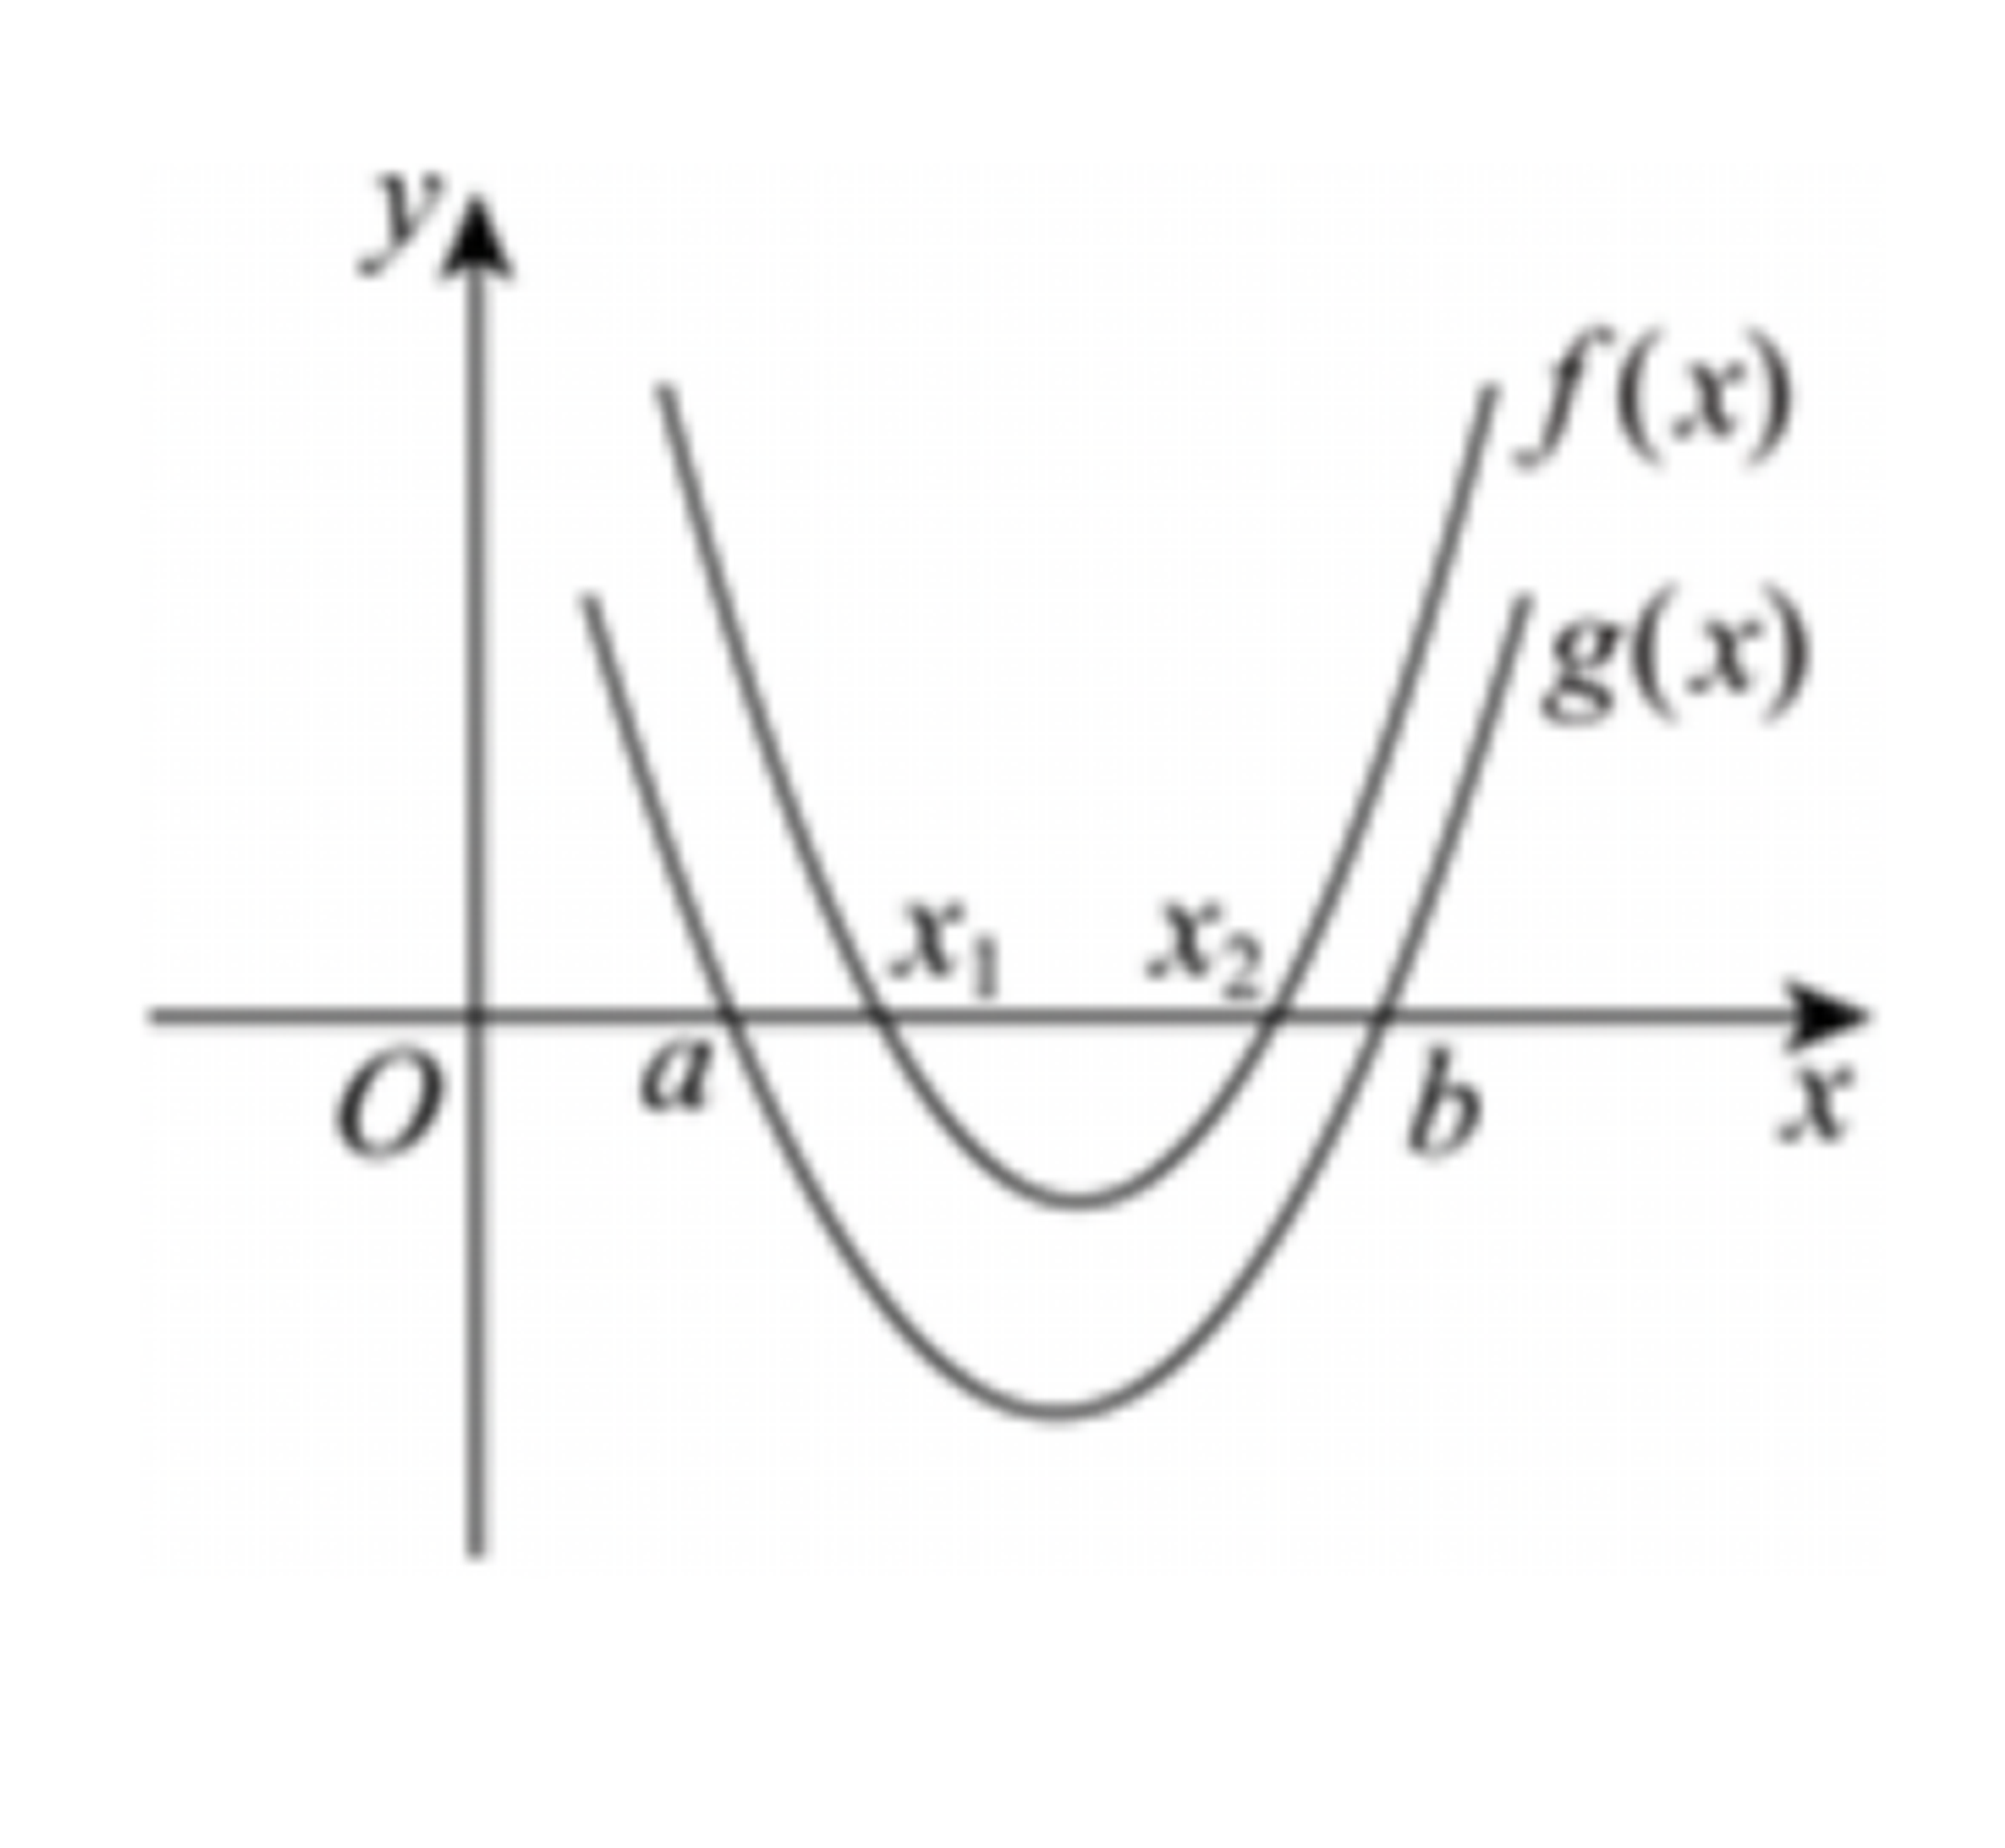
\includegraphics[width=0.30\textwidth]{figures/parabola_f_g_x1x2_h65.png}
\end{center}
\step{由图像得 $a<x_1<x_2<b$，故选 $B$.}
\solend
\fi

\end{enumerate}

\bigsec{三、解答题}

\begin{enumerate}
\setcounter{enumi}{16}

\item 已知 $a>0$，$b>0$，若 $a+b>4$，求证：$\dfrac a{b+2}$ 和 $\dfrac b{a+2}$ 中至少有一个大于 $\dfrac12$.

\ifanswer
\solbegin
\step{假设 $\dfrac a{b+2}\leqslant\dfrac12$，$\dfrac b{a+2}\leqslant\dfrac12$，}
\step{$a>0$，$b>0$，则 $a+2>0$，$b+2>0$，故 $2a\leqslant b+2$，$2b\leqslant a+2$，}
\step{两式相加得 $a+b\leqslant4$，与 $a+b>4$ 矛盾，故 $\dfrac a{b+2}$ 和 $\dfrac b{a+2}$ 中至少有一个大于 $\dfrac12$.}
\solend
\fi

\ansspace[6]

\item 已知集合 $A=\{x\mid-4<x<5\}$，$B=\{x\mid x\leqslant a-6\text{ 或 }x\geqslant a+2\}$.

\begin{enumerate}[label=(\arabic*)]

\item 若 $A\cup B=\R$，求实数 $a$ 的取值范围；

\item 若“$x\in A$”是“$x\in B$”的充分不必要条件，求实数 $a$ 的取值范围.

\end{enumerate}

\ifanswer
\solbegin
\stepm{(1)}{集合 $A=\{x\mid-4<x<5\}$，$B=\{x\mid x\leqslant a-6\text{ 或 }x\geqslant a+2\}$.}
\step{由 $A\cup B=\R$ 得 $\begin{cases}a-6\geqslant-4\\ a+2\leqslant5\end{cases}$，解得 $2\leqslant a\leqslant3$，$a$ 的取值范围为 $[2,3]$；}
\stepm{(2)}{若“$x\in A$”是“$x\in B$”的充分不必要条件，则 $A\subset B$，}
\step{则 $5\leqslant a-6$ 或 $-4\geqslant a+2$，解得 $a\leqslant-6$ 或 $a\geqslant11$.}
\solend
\fi

\ansspace[8]

% 注：原卷题干把命题 $P$ 印作“$\exists3\notin A$”（多一个存在量词），而【解析】两处均作
%     “$3\notin A$”；照录未改，见文件头“原卷笔误/存疑”③。
\item 已知集合 $A=\left\{x\mid\dfrac{x-1}{x-m}<0\right\}$，集合 $B=\left\{x\mid\left|\dfrac{x-1}{x-3}\right|\geqslant1\right\}$，命题 $P$：“$\exists3\notin A$”，命题
$Q$：$A\cap B\neq\varnothing$.

\begin{enumerate}[label=(\arabic*)]

\item 若命题 $P$ 为真命题，求 $m$ 的取值范围；

\item 若命题 $P$ 和命题 $Q$ 至少有一个为假命题，求实数 $m$ 的取值范围.

\end{enumerate}

\ifanswer
\solbegin
\stepm{(1)}{$A=\left\{x\mid\dfrac{x-1}{x-m}<0\right\}=\{x\mid(x-1)(x-m)<0\}$，}
\step{若命题 $P$：“$3\notin A$”为真命题，则 $(3-1)(3-m)\geqslant0$，解得 $m\leqslant3$，}
\step{故实数 $m$ 的取值范围为 $(-\infty,3]$；}
\stepm{(2)}{$B=\left\{x\mid\left|\dfrac{x-1}{x-3}\right|\geqslant1\right\}$，由 $\left|\dfrac{x-1}{x-3}\right|\geqslant1$，得 $\begin{cases}|x-1|\geqslant|x-3|\\ x\neq3\end{cases}$，}
\step{等价于 $\begin{cases}(x-1)^2\geqslant(x-3)^2\\ x\neq3\end{cases}$，解得 $x\geqslant2$ 且 $x\neq3$，所以 $B=[2,3)\cup(3,+\infty)$，}
\step{因为 $A=\{x\mid(x-1)(x-m)<0\}$，}
\step{当 $m=1$ 时，$A=\varnothing$，不满足 $A\cap B\neq\varnothing$，}
\step{当 $m<1$ 时，$A=(m,1)$，不满足 $A\cap B\neq\varnothing$，}
\step{当 $m>1$ 时，$A=(1,m)$，要使 $A\cap B\neq\varnothing$，则 $m>2$，}
\step{则若命题 $Q$：“$A\cap B\neq\varnothing$”为真命题时，实数 $m$ 的取值范围为 $(2,+\infty)$，}
\step{当命题 $P$ 与命题 $Q$ 都是真命题时，则 $\begin{cases}m\leqslant3\\ m>2\end{cases}$，解得 $2<m\leqslant3$，}
\step{则命题 $P$ 和命题 $Q$ 至少有一个为假命题时，得 $m\leqslant2$ 或 $m>3$，}
\step{故实数 $m$ 的取值范围为 $(-\infty,2]\cup(3,+\infty)$.}
\solend
\fi

\ansspace[8]

\item 已知函数 $y=ax^2-(a+2)x+2$，$a\in\R$.

\begin{enumerate}[label=(\arabic*)]

\item $y<3-2x$ 恒成立，求实数 $a$ 的取值范围；

% 注：原卷末句作“求实数 $a$ 的取值”（疑脱“范围”二字），照录未改，
%     见文件头“原卷笔误/存疑”⑤。
\item 若存在 $m>0$ 使关于 $x$ 的方程 $ax^2-(a+2)|x|+2=m+\dfrac1m+1$ 有四个不同的实根，
求实数 $a$ 的取值.

\end{enumerate}

\ifanswer
\solbegin
\stepm{(1)}{由题意得 $ax^2-(a+2)x+2<3-2x$ 恒成立，}
\step{即 $ax^2-ax-1<0$ 恒成立，}
\step{当 $a=0$ 时，$-1<0$ 恒成立，符合题意，}
\step{当 $a\neq0$ 时，则 $\begin{cases}a<0\\ \triangle=a^2+4a<0\end{cases}$，得 $\begin{cases}a<0\\ -4<a<0\end{cases}$，得 $-4<a<0$，}
\step{综上，$a$ 的取值范围为 $(-4,0]$.}
\stepm{(2)}{当 $m>0$ 时，令 $t=m+\dfrac1m+1\geqslant2\sqrt{m\times\dfrac1m}+1=3$，}
\step{当且仅当 $m=1$ 时取等号，}
% 注：题干只给“函数 $y=ax^2-(a+2)x+2$”，全卷未设 $f$，此处 $f(|x|)$ 无定义；
%     照录未改，见文件头“原卷笔误/存疑”④。
\step{则关于 $x$ 的方程 $f(|x|)=t$ 可化为 $a|x|^2-(a+2)|x|+2-t=0$，}
\step{关于 $x$ 的方程为 $a|x|^2-(a+2)|x|+2-t=0$ 有四个不等的实数根，}
\step{即 $ax^2-(a+2)x+2-t=0$，有两个不同的实数正根，}
\step{则 $\begin{cases}\triangle=(a+2)^2-4a(2-t)>0\\ \dfrac{a+2}a>0\\ \dfrac{2-t}a>0\end{cases}$，解得 $a<-2$，}
\step{由（1）得存在 $t\in[3,+\infty)$ 使得不等式 $4at+(a+2)^2-8a>0$ 成立，}
\step{故 $4a\times3+(a+2)^2-8a>0$，即 $a^2+8a+4>0$，}
\step{解得 $a<-4-2\sqrt3$ 或 $a>-4+2\sqrt3$，}
\step{综上，$a<-4-2\sqrt3$，所以 $a$ 的取值范围为 $(-\infty,-4-2\sqrt3)$.}
\solend
\fi

\ansspace[8]

\item 若集合 $A=B_1\cup B_2\cup\cdots\cup B_n$，其中 $B_1$、$B_2$、$\cdots$、$B_n$ 为非空集合，
$B_i\cap B_j=\varnothing$($1\leqslant i<j\leqslant n$)，则称集合 $\{B_1,B_2,\cdots,B_n\}$ 为集合 $A$ 的一个 $n$ 划分.

\begin{enumerate}[label=(\arabic*)]

\item 写出集合 $A=\{1,2,3\}$ 的所有不同的 2 划分；

\item 设 $\{B_1,B_2\}$ 为有理数集 $\Q$ 的一个 2 划分，且满足对任意 $x\in B_1$，任意 $y\in B_2$，都有
$x<y$，判断命题“$B_1$ 中的元素存在最大值，$B_2$ 中的元素存在最小值.”的真假，并说明
理由.

\item 设集合 $A=\{1,2,3,\cdots,16\}$，对于集合 $A$ 的任意一个 3 划分 $\{B_1,B_2,B_3\}$，判断是否存
在 $i\in\{1,2,3\}$，存在 $a$、$b\in B_i$，使得 $b-a\in B_i$ 成立，并说明理由.

\end{enumerate}

\ifanswer
\solbegin
% 注：原卷三个“2 划分”本有外层花括号（$\{\{1,2\},\{3\}\}$ 等），首轮误脱；
%     第二轮复核照原卷补回（原卷原样 / 本稿原错处：原脱外层花括号）。
\stepm{(1)}{集合 $A=\{1,2,3\}$ 的所有不同的 2 划分为 $\{\{1,2\},\{3\}\}$、$\{\{1,3\},\{2\}\}$、}
\step{$\{\{2,3\},\{1\}\}$.}
\stepm{(2)}{该命题为假命题，理由如下：}
\step{假设命题为真，则不妨设 $B_1$ 中元素的最大值为 $s$，$B_2$ 中元素的最小值为 $t$，}
\step{由题意得 $s<t$，所以 $s<\dfrac{s+t}2<t$，}
\step{因为 $s$ 为 $B_1$ 中元素的最大值，所以 $\dfrac{s+t}2\notin B_1$，}
\step{因为 $t$ 为 $B_2$ 中元素的最小值，所以 $\dfrac{s+t}2\notin B_2$，}
\step{因为 $B_1\cup B_2=\Q$，所以 $\dfrac{s+t}2\notin\Q$，}
\step{这与 $\dfrac{s+t}2\in\Q$ 矛盾，所以假设不成立，即命题不可能成立；}
\stepm{(3)}{由于集合 $A$ 中有 16 个元素，}
\step{所以 $B_1$、$B_2$、$B_3$ 中至少有一个集合至少包含 6 个元素，}
\step{不妨设 $B_1$ 中至少包含 6 个元素，}
\step{设 $b_1$、$b_2$、$b_3$、$b_4$、$b_5$、$b_6\in B_1$，且 $b_1<b_2<b_3<b_4<b_5<b_6$，}
\step{假设对任意 $i\in\{1,2,3\}$，对任意 $a$、$b\in B_i$，都有 $b-a\notin B_i$，}
\step{那么 $b_6-b_1$、$b_6-b_2$、$b_6-b_3$、$b_6-b_4$、$b_6-b_5\notin B_1$，}
\step{又因为 $b_6-b_1$、$b_6-b_2$、$b_6-b_3$、$b_6-b_4$、$b_6-b_5\in A$，}
\step{所以 $b_6-b_1$、$b_6-b_2$、$b_6-b_3$、$b_6-b_4$、$b_6-b_5\in B_2\cup B_3$，}
\step{则 $B_2$、$B_3$ 中必有一个集合}
\step{至少包含 $b_6-b_1$、$b_6-b_2$、$b_6-b_3$、$b_6-b_4$、$b_6-b_5$ 中的 3 个元素，}
\step{不妨设这 3 个元素为 $a_1$、$a_2$、$a_3\in B_2$，$a_1<a_2<a_3$，}
\step{由假设得 $a_3-a_1$、$a_3-a_2$、$a_2-a_1\notin B_2$，}
\step{对任意 $i$、$j$($1\leqslant j<i\leqslant3$)，存在 $m$、$n$($1\leqslant m<n\leqslant5$)，}
\step{都有 $a_i-a_j=b_6-b_m-b_6+b_n=b_n-b_m\notin B_1$，}
\step{又因为 $a_3-a_1$、$a_3-a_2$、$a_2-a_1\in B_3$，而 $a_3-a_1-(a_3-a_2)=a_2-a_1$，}
\step{与假设矛盾，所以假设不成立，}
\step{即存在 $i\in\{1,2,3\}$，存在 $a$、$b\in B_i$，使得 $b-a\in B_i$.}
\solend
\fi

\ansspace*[10]

\end{enumerate}

\end{document}
"
% 紧凑版：xelatex "\def\iscompact{1}% 高一65_大同中学_10月月考.tex
%   —— 高一上数学“2026-2027 年大同中学高一上 10 月月考”（讲评版）
% 试卷版：xelatex 高一65_大同中学_10月月考.tex
% 答案版：xelatex "\def\isanswer{1}\input{高一65_大同中学_10月月考.tex}"
% 紧凑版：xelatex "\def\iscompact{1}\input{高一65_大同中学_10月月考.tex}"
%
% 原始材料：微信公众号“魔都数学加油站”文章，作者破晓，连载“27学年高一65”；
% 原文标题“27学年高一65——2026-2027年上海市大同中学高一上10月月考”；
% 原文链接：https://mp.weixin.qq.com/s/h9ctuk-ByE1Vfg2Rx2C6bw。
% 页面标注发布时间 2026-10-17 21:58（上海）。
% 本次转录只据 `原图/高一65_大同中学_10月月考/` 的 11 张 PNG 逐页读图。
% 正文为 11 张 PNG 页（`01..11.png`）：
% 第 06、11 页 2560×3620，第 01、02、03、04、05、07、08、09、10 页 4762×6735
% （**同一篇各页分辨率不同**），均按页序读取。11 页全为试卷正文页（卷首标题在第 1 页页顶，
% 卷末解答题第 21 题解析止于第 11 页），无封面页、目录页、二维码或宣传页。
% 粉色斜排“魔都数学加油站”为卷面水印，与公众号页脚一并未录入。
%
% 卷首标题：照卷面印作“2026--2027 年大同中学高一上 10 月月考”，年份区间按全稿惯例排 en dash。
% 原卷只有一行标题、无副标题。
%
% 篇幅与题号：原卷自第 3 题起编号（第 1、2 题不在本卷内）。填空题 3—12（10 题）、
% 选择题 13—16（4 题）、解答题 17—21（5 题），共 19 题。本稿沿用原节与原题号，
% 只改排为全稿统一的大节样式（原卷小节标题为“一、填空题”“二、选择题”“三、解答题”）。
%
% 讲评版：原卷每题下直接印【答案】或【解析】。**只印【答案】的 4 题**（第 3、4、7、10 题），
% 本稿只给 \ans{}；其余 15 题都印【解析】（按全稿口径这类题不另提 \ans{}——第 12、13、14、
% 15、16 题的结论写在解析末句（“故选 B”“综上，n 的最大值为 14”等），亦照录在解析内）。
% 全卷无“答案印在题干括号内”的题（第 13—16 题的选择题括号内均空白）。
%
% 副标题：原卷未印副标题。本稿按“知识模块”口径标作“集合与常用逻辑用语、不等式”：
% 19 题中集合与常用逻辑用语 10 题（第 3、4、6、8、12、14、15、18、19、21 题），
% 不等式 9 题（含等式恒等、不等式性质、二次不等式、恒成立、基本不等式、不等式的证明：
% 第 5、7、9、10、11、13、16、17、20 题），两类均超过三分之一，故并标。口径同 高一63。
%
% 与原卷的排版差异：
%   ① 原卷每题下直接印【答案】/【解析】，本稿按全稿惯例将答案与解析置于答案版，试卷版保持干净；
%   ② 原卷未印副标题，本稿按“知识模块”口径补出；
%   ③ 原卷填空横线约四个字宽，本稿按全稿惯例统一排 \blankline[4.4em]；
%   ④ 原卷数集记号全为斜体：实数集作 $R$（第 6 题两处、第 8 题两处、第 15 题解析、第 18 题、
%      第 20 题题干），自然数集作 $N$（第 12 题题干“$n\in N,n\geqslant1$”），有理数集作 $Q$
%      （第 21 题 (2) 题干与解析共 4 处），本稿按全稿惯例统一改用 $\R$、$\N$、$\Q$
%      （同 高一63 排版差异④：记号归一）；空集记号原卷作 $\varnothing$，照录；
%   ⑤ 原卷用描述法时竖线排细竖“$|$”（如 $\{x|0<x<3\}$、$\{x|(x-1)(x-m)<0\}$），
%      本稿按全稿惯例排 \mid；
%   ⑥ 原卷判别式印作“$\triangle$”（第 8、14 题解析各 1 处、第 20 题解析 2 处，共 4 处），
%      本稿照录用 \triangle（同 高一39 成例），未改作 \Delta；
%   ⑦ 第 18—21 题的子问原卷各自另起一行、以“（1）”“（2）”标号，本稿按全稿惯例用
%      enumerate 的 (1)(2)(3)；解析中的子问标号一律用 \stepm{(1)}{…}；
%      第 18—21 题解析（原文以“（1）”“（2）”“（3）”冠于解析首句）同此；
%   ⑧ 选择题的作答括号原卷排半角“(　　)”（第 13—16 题括号内均空白），
%      本稿按全稿惯例排 \mbox{（\quad）}；选项字母后的句点照原卷排“A.”“B.”；
%   ⑨ 每道解答题原卷未留作答空白，本稿按全稿惯例加 \ansspace（末题用 \ansspace*）；
%   ⑩ 原卷在数学式内多处用半角逗号（如 $\{x|0<x<3\},B=\{x|x>2\}$、$m\in I_{14},k\in I_{14}$），
%      均照录未强改；句末句点按全稿惯例排西文句点。
%
% 原卷笔误/存疑（均照录未改，正文对应处另有 % 注）：
%   ① 第 13 题题干“下列不等式中一定成立是（　　）”脱一个“的”（当作“一定成立的是”），
%      8 倍放大确认非水印遮挡，本稿照录；
%   ② 第 15 题【解析】末段把题干条件“$x\geqslant10$”写成“$x\geqslant1$”
%      （“所以 $x+2+\frac{16}{x+2}(x\geqslant1)$ 的最小值不为 8”），与同段前面“令 $t=x+2$，
%      则 $t\geqslant12$”不合，本稿照录；
%   ③ 第 19 题题干把命题 $P$ 印作“$\exists3\notin A$”（多一个存在量词），而【解析】两处
%      均作“$3\notin A$”，前后记号不一，本稿照录；
%   ④ 第 20 题【解析】(2) 出现 $f(|x|)$，但题干只给“函数 $y=ax^2-(a+2)x+2$”、全卷未设 $f$，
%      本稿照录；
%   ⑤ 第 20 题 (2) 题干末句作“求实数 $a$ 的取值”（疑脱“范围”二字），本稿照录；
%   ⑥ 第 12 题【解析】第 18 步“它与 $P_n$ 中的任何其他数之和都不是整数”，该段所论为 $P_{14}$
%      （前后均作 $P_{14}$），此处 $P_n$ 疑当作 $P_{14}$，本稿照录。
%
% 第二轮复核（2026-10-18）订正「本稿抄错原卷」一处：
%   第 21 题 (1)【解析】原卷本作“$\{\{1,2\},\{3\}\}$、$\{\{1,3\},\{2\}\}$、$\{\{2,3\},\{1\}\}$”，
%   有外层花括号；首轮误脱外层花括号，并曾在文件头误记为“原卷未加外层花括号”（原第 ⑦ 条，
%   已撤销）。本次照原卷补回，正文对应处另有 % 注。
%
% 插图：第 16 题【解析】内有 1 幅图（两条开口向上的抛物线 $f(x)$、$g(x)$ 与 $x$ 轴交点
% 标 $a$、$x_1$、$x_2$、$b$，纵轴标 $y$、原点 $O$），解析第三行“画出函数 $g(x)$ 与函数 $f(x)$
% 的图像，如图所示”即指此图；取原卷截图（06.png，2560×3620）右半幅，4× LANCZOS 放大，
% 存 figures/parabola_f_g_x1x2_h65.png。该图在【解析】内，仅答案版出。
%
\documentclass[a4paper,11pt]{article}
\usepackage{common}

\begin{document}

\examtitlest[3]{2026--2027 年大同中学高一上 10 月月考}{集合与常用逻辑用语、不等式}

\bigsec{一、填空题}

\begin{enumerate}
\setcounter{enumi}{2}

\item 已知集合 $A=\{x\mid0<x<3\}$,$B=\{x\mid x>2\}$，则集合 $A\cup B=$\blankline[4.4em].

\ifanswer
\ans{$(0,+\infty)$}
\fi

\item “$x>1$ 或 $y>1$”的否定形式是\blankline[4.4em].

\ifanswer
\ans{$x\leqslant1$ 且 $y\leqslant1$}
\fi

\item 已知等式 $2x^2+3x+4=a(2x+1)(x+1)+b$ 恒成立，则常数 $a-b=$\blankline[4.4em].

\ifanswer
\solbegin
\step{因为等式 $2x^2+3x+4=a(2x+1)(x+1)+b$ 恒成立，}
\step{所以 $a(2x+1)(x+1)+b=2ax^2+3ax+a+b=2x^2+3x+4$，}
\step{所以 $\begin{cases}2a=2\\ 3a=3\\ a+b=4\end{cases}$，解得 $\begin{cases}a=1\\ b=3\end{cases}$，所以 $a-b=-2$.}
\solend
\fi

\item 全集为 $U=\R$，$A=\{x\mid|x|\geqslant2\}$，$B=\{y\mid y=x^2+1,x\in\R\}$，则 $A\cup\bar B=$\blankline[4.4em].

\ifanswer
\solbegin
\step{由题意得集合 $A=\{x\mid x\geqslant2\text{ 或 }x\leqslant-2\}$，}
\step{因为 $x^2+1\geqslant1$，所以集合 $B=\{x\mid x\geqslant1\}$，所以 $\bar B=\{x\mid x<1\}$，}
\step{则 $A\cup\bar B=\{x\mid x\geqslant2\text{ 或 }x<1\}$.}
\solend
\fi

\item 已知 $|x+3|+|x-5|=8$，则实数 $x$ 的取值范围为\blankline[4.4em].

\ifanswer
\ans{$[-3,5]$}
\fi

\item 已知集合 $A=\{x\in\R\mid ax^2+2x+1=0,a\in\R\}$ 只有一个元素，则 $a$ 的值为\blankline[4.4em].

\ifanswer
\solbegin
\step{当 $a=0$ 时，$A=\left\{-\dfrac12\right\}$；}
\step{当 $a\neq0$ 时，若集合 $A$ 只有一个元素，由 $\triangle=4-4a=0$ 得 $a=1$.}
\step{综上，当 $a=0$ 或 $a=1$ 时，集合 $A$ 只有一个元素.}
\solend
\fi

\item 已知不等式 $-x^2+bx+c>0$ 的解集为 $(3,4)$，则不等式 $cx^2+bx-1<0$ 的解集为\blankline[4.4em].

\ifanswer
\solbegin
\step{由题意得 3，4 是方程 $-x^2+bx+c=0$ 的两个实数根，}
\step{所以 $\begin{cases}3+4=b\\ 3\times4=-c\end{cases}$，得 $b=7$，$c=-12$，}
\step{则不等式 $cx^2+bx-1<0$，即为 $-12x^2+7x-1<0$，即 $12x^2-7x+1>0$，}
\step{化简得 $(3x-1)(4x-1)>0$，解得 $x<\dfrac14$ 或 $x>\dfrac13$，}
\step{即不等式 $cx^2+bx-1<0$ 的解集为 $\left(-\infty,\dfrac14\right)\cup\left(\dfrac13,+\infty\right)$.}
\solend
\fi

\item 对于区间 $(m,n)$，我们将 $n-m$ 的值称为该区间的长度. 若关于 $x$ 的不等式
$x^2+ax+a<0$ 有解，且解集的区间长度不超过 $2\sqrt3$，则实数 $a$ 的取值范围是\blankline[4.4em].

\ifanswer
\ans{$[-2,0)\cup(4,6]$}
\fi

\item 当 $x>0$ 时，关于 $x$ 的不等式 $(ax-1)(x^2+bx-4)\geqslant0$ 恒成立，则 $b+\dfrac2a$ 的最小值
为\blankline[4.4em].

\ifanswer
\solbegin
\step{由题意 $a\neq0$；}
\step{若 $a<0$，则 $x>0$ 时 $ax-1<0$ 恒成立，需 $x^2+bx-4\leqslant0$ 对一切 $x>0$ 成立，}
\step{而 $y=x^2+bx-4$ 的图象开口向上，当 $x$ 充分大时必为正值，矛盾，故 $a>0$.}
\step{当 $a>0$ 时，$ax-1=a\left(x-\dfrac1a\right)$，故原条件化为 $\left(x-\dfrac1a\right)(x^2+bx-4)\geqslant0$：}
\step{若 $0<x<\dfrac1a$，则 $x-\dfrac1a<0$，需 $x^2+bx-4\leqslant0$；}
\step{若 $x>\dfrac1a$，则 $x-\dfrac1a>0$，需 $x^2+bx-4\geqslant0$；}
\step{由 $y=x^2+bx-4$ 的连续性知 $x=\dfrac1a$ 是它的零点，}
\step{即 $\dfrac1{a^2}+\dfrac ba-4=0$，得 $b=4a-\dfrac1a$；}
\step{此时 $x^2+bx-4=x^2+\left(4a-\dfrac1a\right)x-4=(x+4a)\left(x-\dfrac1a\right)$，}
\step{由 $a>0$、$x>0$ 得 $x+4a>0$，}
\step{其符号与 $x-\dfrac1a$ 一致，故能与 $ax-1$ 同号，原不等式确在 $x>0$ 上恒成立.}
\step{于是 $b+\dfrac2a=4a-\dfrac1a+\dfrac2a=4a+\dfrac1a\geqslant2\sqrt{4a\cdot\dfrac1a}=4$，}
\step{当且仅当 $a=\dfrac12$ 时取等号，故最小值为 4.}
\solend
\fi

\item 设集合 $I_n=\{1,2,\cdots,n\}$，$n\in\N$，$n\geqslant1$，集合 $P_n=\left\{\dfrac m{\sqrt k}\mid m\in I_n,k\in I_n\right\}$，若 $P_n$ 的子集 $A$
中任意两个元素之和不是整数的平方，则称 $A$ 为“人文集”. 那么使 $P_n$ 能分成两个交集为空
集的“人文集”的并集，且这两个人文集的并集恰为 $P_n$ 时，$n$ 的最大值是\blankline[4.4em].

\ifanswer
\solbegin
\step{先证当 $n\geqslant15$ 时，$P_n$ 不能分成两个不相交的人文集的并集.}
\step{假设当 $n\geqslant15$ 时，$P_n$ 可以分成两个不相交的人文集的并集，}
\step{设 $A$ 和 $B$ 为两个不相交的人文集，使 $A\cup B=P_n\supseteq I_n$.}
\step{不妨设 $1\in A$，则由于 $1+3=2^2$，所以 $3\notin A$，即 $3\in B$.}
\step{同理可得，$6\in A$，$10\in B$. 又推出 $15\in A$，}
\step{但 $1+15=4^2$，这与 $A$ 为人文集相矛盾.}
\step{再证 $P_{14}$ 满足要求. 当 $k=1$ 时，$P_{14}=\left\{\dfrac m{\sqrt k}\mid m\in I_{14},k\in I_{14}\right\}$，}
\step{可以分成 2 个人文集的并集.}
\step{事实上，只要取 $A_1=\{1,2,4,6,9,11,13\}$，$B_1=\{3,5,7,8,10,12,14\}$，}
\step{则 $A_1$ 和 $B_1$ 都是人文集，且 $A_1\cup B_1=P_{14}$.}
\step{当 $k=4$ 时，集合 $\left\{\dfrac m{\sqrt k}\mid m\in I_{14}\right\}$ 中，除整数外，}
\step{剩下的数组成集合 $\left\{\dfrac12,\dfrac32,\dfrac52,\cdots,\dfrac{13}2\right\}$，}
\step{可以分为下列 2 个人文集的并：$A_2=\left\{\dfrac12,\dfrac52,\dfrac92,\dfrac{11}2\right\}$，$B_2=\left\{\dfrac32,\dfrac72,\dfrac{13}2\right\}$.}
\step{当 $k=9$ 时，集合 $\left\{\dfrac m{\sqrt k}\mid m\in I_{14}\right\}$ 中，除整数外，}
\step{剩下的数组成集合 $\left\{\dfrac13,\dfrac23,\dfrac43,\dfrac53,\cdots,\dfrac{13}3,\dfrac{14}3\right\}$，}
\step{可以分为下列 2 个人文集的并：$A_3=\left\{\dfrac13,\dfrac43,\dfrac53,\dfrac{10}3,\dfrac{13}3\right\}$，$B_3=\left\{\dfrac23,\dfrac73,\dfrac83,\dfrac{11}3,\dfrac{14}3\right\}$.}
\step{最后，集合 $C=\left\{\dfrac m{\sqrt k}\mid m\in I_{14},k\in I_{14},k\neq1,4,9\right\}$ 中的数的分母都是无理数，}
% 注：本行原卷作“$P_n$”，而该段所论为 $P_{14}$（前后均作 $P_{14}$），疑当作 $P_{14}$；
%     照录未改，见文件头“原卷笔误/存疑”⑥。
\step{它与 $P_n$ 中的任何其他数之和都不是整数，}
\step{因此，令 $A=A_1\cup A_2\cup A_3\cup C$，$B=B_1\cup B_2\cup B_3$，}
\step{则 $A$ 和 $B$ 是不相交的人文集，且 $A\cup B=P_{14}$.}
\step{综上，$n$ 的最大值为 14.}
\solend
\fi

\end{enumerate}

\bigsec{二、选择题}

\begin{enumerate}
\setcounter{enumi}{12}

% 注：原卷题干“下列不等式中一定成立是”脱一个“的”（当作“一定成立的是”），
%     照录未改，见文件头“原卷笔误/存疑”①。
\item 已知 $a>b$，下列不等式中一定成立是\mbox{（\quad）}

\keepwithprev
A. $a^2>b^2$\qquad B. $ac^2>bc^2$\qquad C. $\dfrac1a<\dfrac1b$\qquad D. $a+3>b-4$

\ifanswer
\solbegin
\step{对于 $A$，当 $a=-2$，$b=-4$ 时，不等式不成立，故 $A$ 错误；}
\step{对于 $B$，当 $c=0$ 时，不等式不成立，故 $B$ 错误；}
\step{对于 $C$，当 $a=2$，$b=-4$ 时，不等式不成立，故 $C$ 错误；}
\step{对于 $D$，因为 $a>b$，$3>-4$，必有 $a+3>b-4$ 成立，故 $D$ 正确.}
\step{故选 $D$.}
\solend
\fi

\item 已知 $a$ 为实数，那么“$|a|\leqslant2$”是“方程 $x^2+ax+1=0$ 没有实数解”的\mbox{（\quad）}

\keepwithprev
A. 充分而不必要条件\qquad B. 必要而不充分条件

C. 充要条件\qquad D. 既不充分也不必要条件

\ifanswer
\solbegin
\step{由方程 $x^2+ax+1=0$ 没有实数解，得 $\triangle=a^2-4<0$，则 $|a|<2$，}
\step{由 $|a|<2$ 得 $|a|\leqslant2$，反之不成立，}
\step{所以“$|a|\leqslant2$”是“方程 $x^2+ax+1=0$ 没有实数解”的必要而不充分条件.}
\step{故选 $B$.}
\solend
\fi

\item 下列命题为真命题的是\mbox{（\quad）}

\keepwithprev
A. $a>b>0$，当 $m>0$ 时，$\dfrac{a+m}{b+m}>\dfrac ab$

B. 集合 $A=\{x\mid y=x^2+1\}$ 与集合 $B=\{y\mid y=x^2+1\}$ 是相同的集合

C. 若 $b<a<0$，$m<0$，则 $\dfrac ma>\dfrac mb$

D. $x+2+\dfrac{16}{x+2}(x\geqslant10)$ 最小值为 8

\ifanswer
\solbegin
\step{对于 $A$，$\dfrac{a+m}{b+m}-\dfrac ab=\dfrac{b(a+m)-a(b+m)}{b(b+m)}=\dfrac{m(b-a)}{b(b+m)}$，}
\step{因为 $a>b>0$，$m>0$，所以 $b(b+m)>0$，$m(b-a)<0$，}
\step{所以 $\dfrac{a+m}{b+m}-\dfrac ab=\dfrac{m(b-a)}{b(b+m)}<0$，}
\step{即 $a>b>0$，当 $m>0$ 时，$\dfrac{a+m}{b+m}<\dfrac ab$，故 $A$ 错误；}
\step{对于 $B$，集合 $A=\{x\mid y=x^2+1\}=\R$，集合 $B=\{y\mid y=x^2+1\}=\{y\mid y\geqslant1\}$，}
\step{所以 $A\neq B$，故 $B$ 错误；}
\step{对于 $C$，$\dfrac ma-\dfrac mb=\dfrac{m(b-a)}{ab}$，}
\step{因为 $b<a<0$，$m<0$，所以 $ab>0$，$m(b-a)>0$，}
\step{所以 $\dfrac ma-\dfrac mb=\dfrac{m(b-a)}{ab}>0$，即 $\dfrac ma>\dfrac mb$，故 $C$ 正确；}
\step{对于 $D$，令 $t=x+2$，则 $t\geqslant12$，表达式变为 $t+\dfrac{16}t$，}
\step{$t+\dfrac{16}t\geqslant2\sqrt{t\cdot\dfrac{16}t}=8$，当且仅当 $t=4$ 时取等号，即等号不成立，}
% 注：原卷本行把题干条件“$x\geqslant10$”写成“$x\geqslant1$”，与同段“$t\geqslant12$”不合；
%     照录未改，见文件头“原卷笔误/存疑”②。
\step{所以 $x+2+\dfrac{16}{x+2}(x\geqslant1)$ 的最小值不为 8，故 $D$ 错误.}
\step{故选 $C$.}
\solend
\fi

\item 已知实数 $a<b$，关于 $x$ 的不等式 $x^2-(a+b)x+ab+\dfrac12<0$ 的解集为 $(x_1,x_2)$，则实数 $a$、
$b$、$x_1$、$x_2$ 从小到大的排列是\mbox{（\quad）}

\keepwithprev
A. $x_1<a<b<x_2$\qquad B. $a<x_1<x_2<b$\qquad C. $a<x_1<b<x_2$\qquad D. $x_1<a<x_2<b$

\ifanswer
\solbegin
\step{不等式 $x^2-(a+b)x+ab+\dfrac12<0$ 可化为 $(x-a)(x-b)+\dfrac12<0$，}
\step{设 $g(x)=(x-a)(x-b)$，$f(x)=g(x)+\dfrac12$，}
\step{画出函数 $g(x)$ 与函数 $f(x)$ 的图像，如图所示，}
% 图在【解析】内（仅答案版出），取原卷截图（06.png，2560×3620）右半幅，4× LANCZOS 放大。
\begin{center}
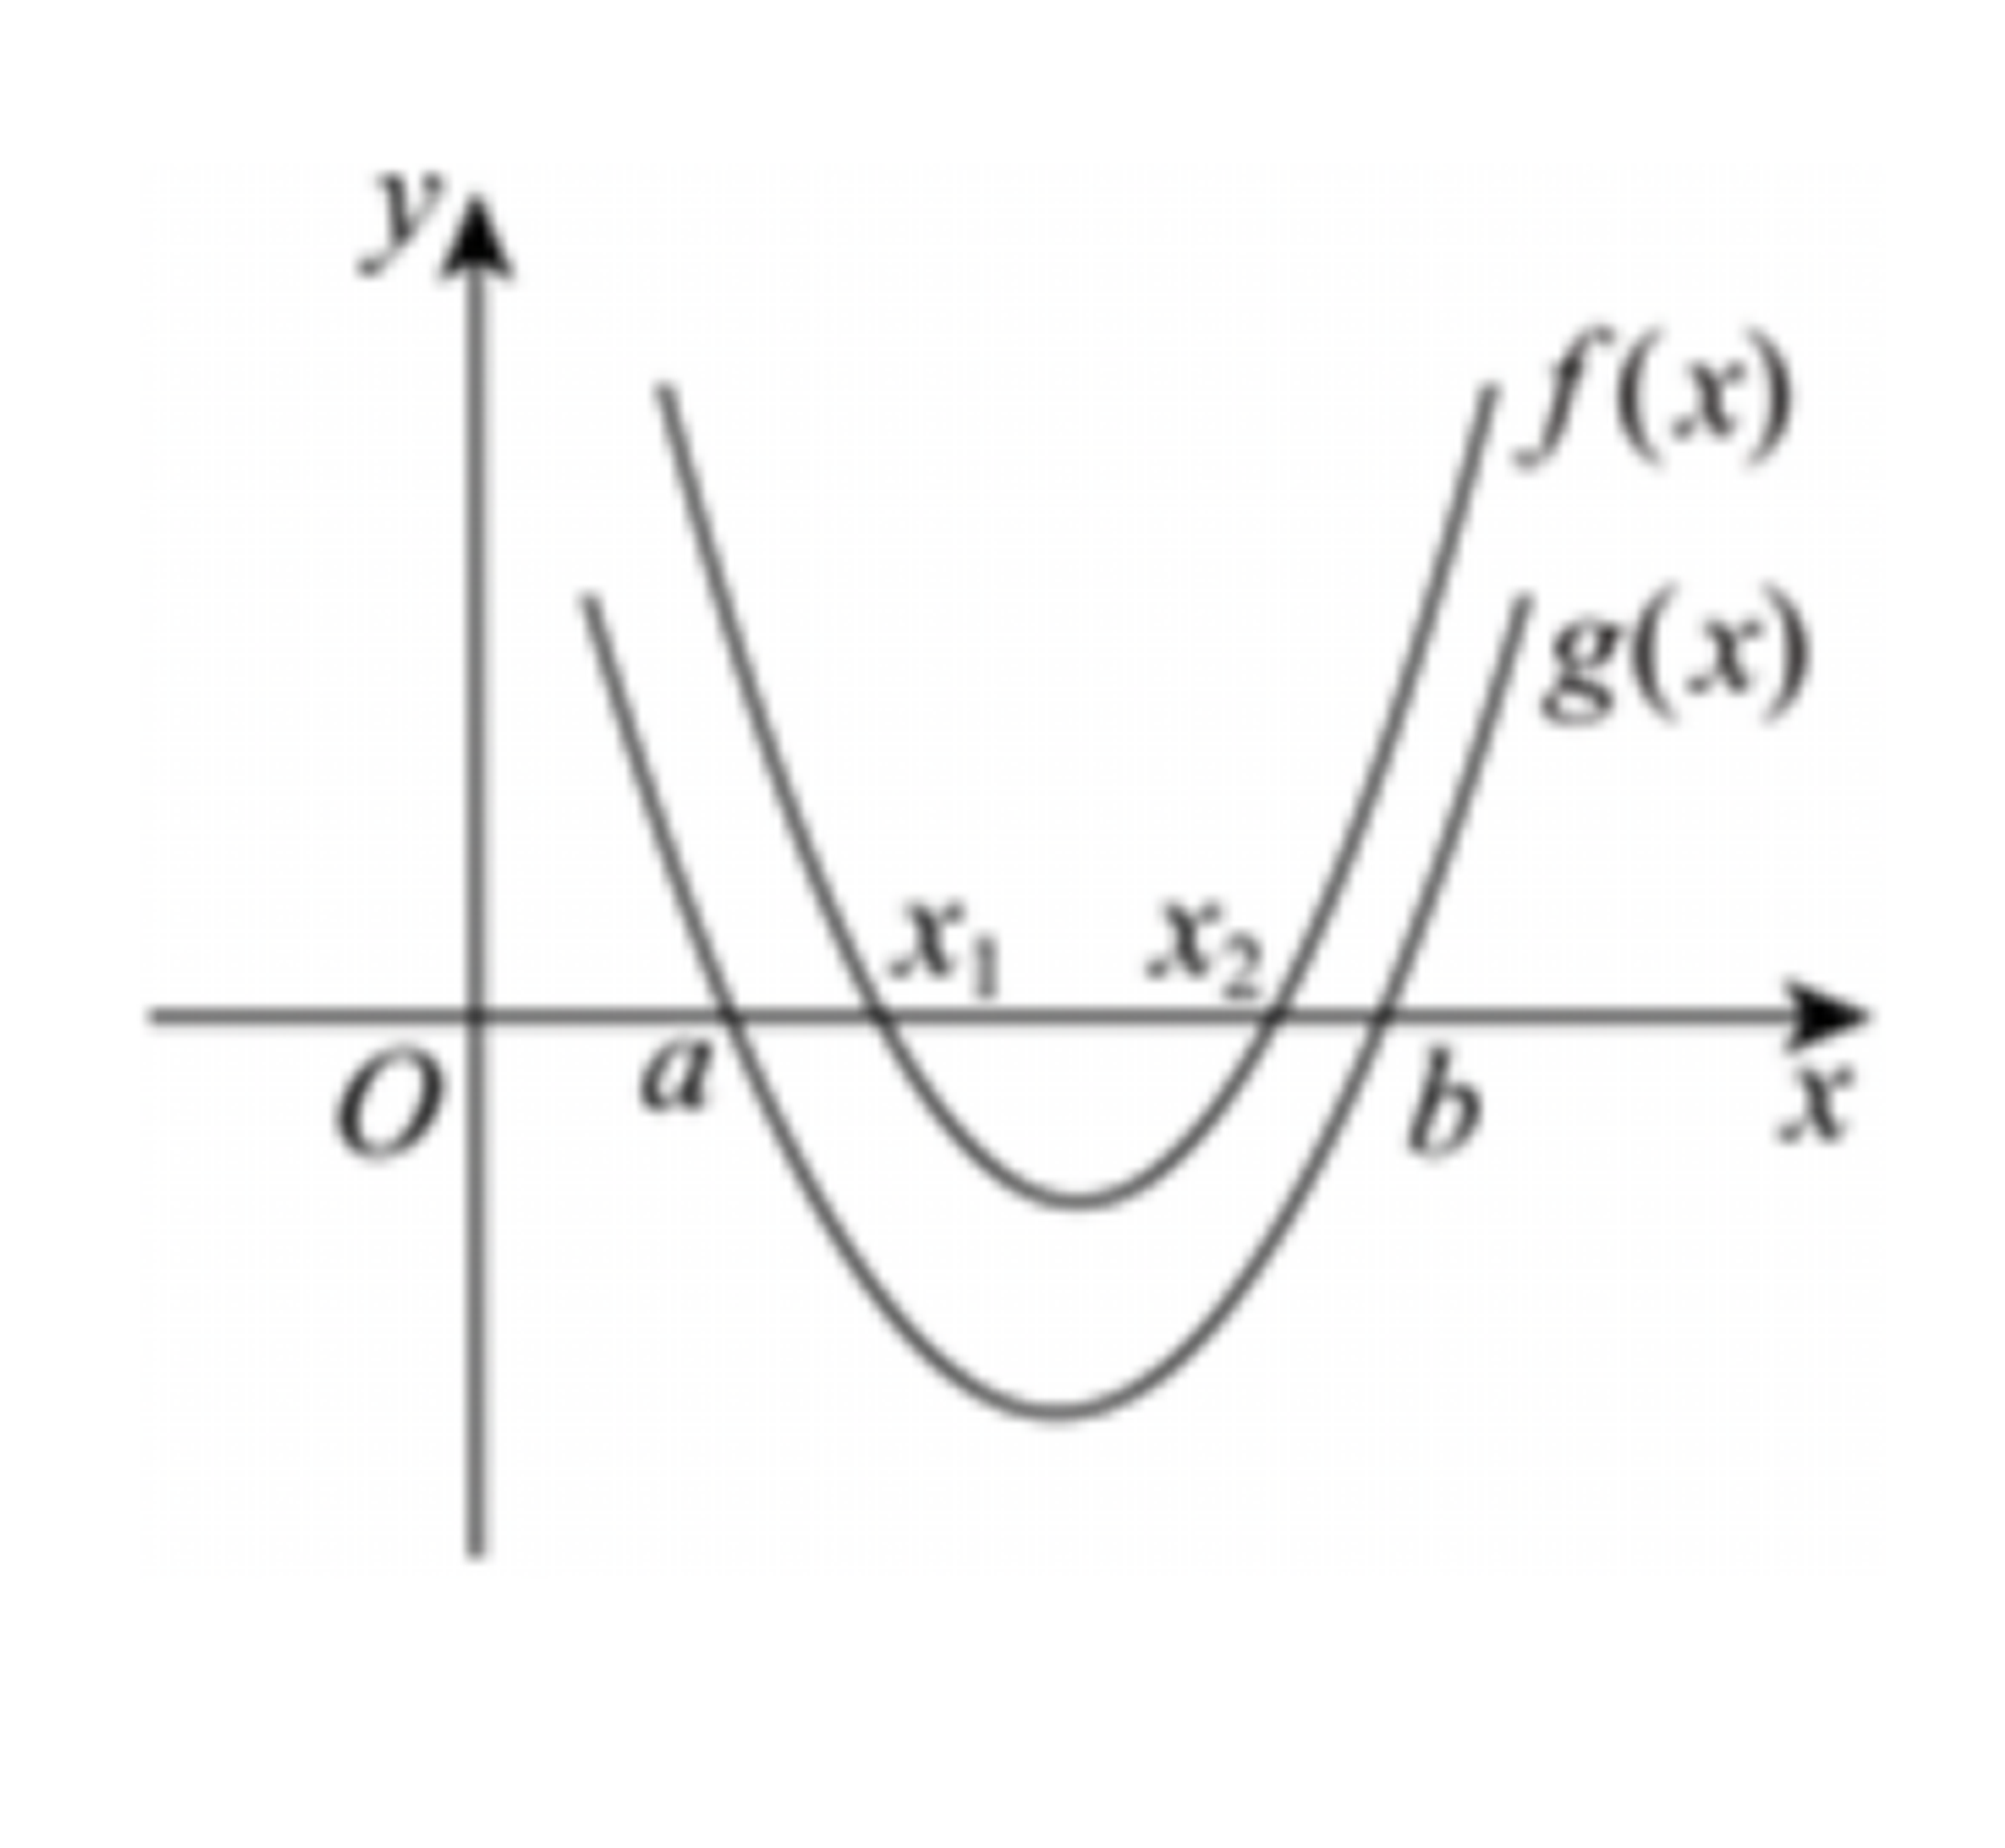
\includegraphics[width=0.30\textwidth]{figures/parabola_f_g_x1x2_h65.png}
\end{center}
\step{由图像得 $a<x_1<x_2<b$，故选 $B$.}
\solend
\fi

\end{enumerate}

\bigsec{三、解答题}

\begin{enumerate}
\setcounter{enumi}{16}

\item 已知 $a>0$，$b>0$，若 $a+b>4$，求证：$\dfrac a{b+2}$ 和 $\dfrac b{a+2}$ 中至少有一个大于 $\dfrac12$.

\ifanswer
\solbegin
\step{假设 $\dfrac a{b+2}\leqslant\dfrac12$，$\dfrac b{a+2}\leqslant\dfrac12$，}
\step{$a>0$，$b>0$，则 $a+2>0$，$b+2>0$，故 $2a\leqslant b+2$，$2b\leqslant a+2$，}
\step{两式相加得 $a+b\leqslant4$，与 $a+b>4$ 矛盾，故 $\dfrac a{b+2}$ 和 $\dfrac b{a+2}$ 中至少有一个大于 $\dfrac12$.}
\solend
\fi

\ansspace[6]

\item 已知集合 $A=\{x\mid-4<x<5\}$，$B=\{x\mid x\leqslant a-6\text{ 或 }x\geqslant a+2\}$.

\begin{enumerate}[label=(\arabic*)]

\item 若 $A\cup B=\R$，求实数 $a$ 的取值范围；

\item 若“$x\in A$”是“$x\in B$”的充分不必要条件，求实数 $a$ 的取值范围.

\end{enumerate}

\ifanswer
\solbegin
\stepm{(1)}{集合 $A=\{x\mid-4<x<5\}$，$B=\{x\mid x\leqslant a-6\text{ 或 }x\geqslant a+2\}$.}
\step{由 $A\cup B=\R$ 得 $\begin{cases}a-6\geqslant-4\\ a+2\leqslant5\end{cases}$，解得 $2\leqslant a\leqslant3$，$a$ 的取值范围为 $[2,3]$；}
\stepm{(2)}{若“$x\in A$”是“$x\in B$”的充分不必要条件，则 $A\subset B$，}
\step{则 $5\leqslant a-6$ 或 $-4\geqslant a+2$，解得 $a\leqslant-6$ 或 $a\geqslant11$.}
\solend
\fi

\ansspace[8]

% 注：原卷题干把命题 $P$ 印作“$\exists3\notin A$”（多一个存在量词），而【解析】两处均作
%     “$3\notin A$”；照录未改，见文件头“原卷笔误/存疑”③。
\item 已知集合 $A=\left\{x\mid\dfrac{x-1}{x-m}<0\right\}$，集合 $B=\left\{x\mid\left|\dfrac{x-1}{x-3}\right|\geqslant1\right\}$，命题 $P$：“$\exists3\notin A$”，命题
$Q$：$A\cap B\neq\varnothing$.

\begin{enumerate}[label=(\arabic*)]

\item 若命题 $P$ 为真命题，求 $m$ 的取值范围；

\item 若命题 $P$ 和命题 $Q$ 至少有一个为假命题，求实数 $m$ 的取值范围.

\end{enumerate}

\ifanswer
\solbegin
\stepm{(1)}{$A=\left\{x\mid\dfrac{x-1}{x-m}<0\right\}=\{x\mid(x-1)(x-m)<0\}$，}
\step{若命题 $P$：“$3\notin A$”为真命题，则 $(3-1)(3-m)\geqslant0$，解得 $m\leqslant3$，}
\step{故实数 $m$ 的取值范围为 $(-\infty,3]$；}
\stepm{(2)}{$B=\left\{x\mid\left|\dfrac{x-1}{x-3}\right|\geqslant1\right\}$，由 $\left|\dfrac{x-1}{x-3}\right|\geqslant1$，得 $\begin{cases}|x-1|\geqslant|x-3|\\ x\neq3\end{cases}$，}
\step{等价于 $\begin{cases}(x-1)^2\geqslant(x-3)^2\\ x\neq3\end{cases}$，解得 $x\geqslant2$ 且 $x\neq3$，所以 $B=[2,3)\cup(3,+\infty)$，}
\step{因为 $A=\{x\mid(x-1)(x-m)<0\}$，}
\step{当 $m=1$ 时，$A=\varnothing$，不满足 $A\cap B\neq\varnothing$，}
\step{当 $m<1$ 时，$A=(m,1)$，不满足 $A\cap B\neq\varnothing$，}
\step{当 $m>1$ 时，$A=(1,m)$，要使 $A\cap B\neq\varnothing$，则 $m>2$，}
\step{则若命题 $Q$：“$A\cap B\neq\varnothing$”为真命题时，实数 $m$ 的取值范围为 $(2,+\infty)$，}
\step{当命题 $P$ 与命题 $Q$ 都是真命题时，则 $\begin{cases}m\leqslant3\\ m>2\end{cases}$，解得 $2<m\leqslant3$，}
\step{则命题 $P$ 和命题 $Q$ 至少有一个为假命题时，得 $m\leqslant2$ 或 $m>3$，}
\step{故实数 $m$ 的取值范围为 $(-\infty,2]\cup(3,+\infty)$.}
\solend
\fi

\ansspace[8]

\item 已知函数 $y=ax^2-(a+2)x+2$，$a\in\R$.

\begin{enumerate}[label=(\arabic*)]

\item $y<3-2x$ 恒成立，求实数 $a$ 的取值范围；

% 注：原卷末句作“求实数 $a$ 的取值”（疑脱“范围”二字），照录未改，
%     见文件头“原卷笔误/存疑”⑤。
\item 若存在 $m>0$ 使关于 $x$ 的方程 $ax^2-(a+2)|x|+2=m+\dfrac1m+1$ 有四个不同的实根，
求实数 $a$ 的取值.

\end{enumerate}

\ifanswer
\solbegin
\stepm{(1)}{由题意得 $ax^2-(a+2)x+2<3-2x$ 恒成立，}
\step{即 $ax^2-ax-1<0$ 恒成立，}
\step{当 $a=0$ 时，$-1<0$ 恒成立，符合题意，}
\step{当 $a\neq0$ 时，则 $\begin{cases}a<0\\ \triangle=a^2+4a<0\end{cases}$，得 $\begin{cases}a<0\\ -4<a<0\end{cases}$，得 $-4<a<0$，}
\step{综上，$a$ 的取值范围为 $(-4,0]$.}
\stepm{(2)}{当 $m>0$ 时，令 $t=m+\dfrac1m+1\geqslant2\sqrt{m\times\dfrac1m}+1=3$，}
\step{当且仅当 $m=1$ 时取等号，}
% 注：题干只给“函数 $y=ax^2-(a+2)x+2$”，全卷未设 $f$，此处 $f(|x|)$ 无定义；
%     照录未改，见文件头“原卷笔误/存疑”④。
\step{则关于 $x$ 的方程 $f(|x|)=t$ 可化为 $a|x|^2-(a+2)|x|+2-t=0$，}
\step{关于 $x$ 的方程为 $a|x|^2-(a+2)|x|+2-t=0$ 有四个不等的实数根，}
\step{即 $ax^2-(a+2)x+2-t=0$，有两个不同的实数正根，}
\step{则 $\begin{cases}\triangle=(a+2)^2-4a(2-t)>0\\ \dfrac{a+2}a>0\\ \dfrac{2-t}a>0\end{cases}$，解得 $a<-2$，}
\step{由（1）得存在 $t\in[3,+\infty)$ 使得不等式 $4at+(a+2)^2-8a>0$ 成立，}
\step{故 $4a\times3+(a+2)^2-8a>0$，即 $a^2+8a+4>0$，}
\step{解得 $a<-4-2\sqrt3$ 或 $a>-4+2\sqrt3$，}
\step{综上，$a<-4-2\sqrt3$，所以 $a$ 的取值范围为 $(-\infty,-4-2\sqrt3)$.}
\solend
\fi

\ansspace[8]

\item 若集合 $A=B_1\cup B_2\cup\cdots\cup B_n$，其中 $B_1$、$B_2$、$\cdots$、$B_n$ 为非空集合，
$B_i\cap B_j=\varnothing$($1\leqslant i<j\leqslant n$)，则称集合 $\{B_1,B_2,\cdots,B_n\}$ 为集合 $A$ 的一个 $n$ 划分.

\begin{enumerate}[label=(\arabic*)]

\item 写出集合 $A=\{1,2,3\}$ 的所有不同的 2 划分；

\item 设 $\{B_1,B_2\}$ 为有理数集 $\Q$ 的一个 2 划分，且满足对任意 $x\in B_1$，任意 $y\in B_2$，都有
$x<y$，判断命题“$B_1$ 中的元素存在最大值，$B_2$ 中的元素存在最小值.”的真假，并说明
理由.

\item 设集合 $A=\{1,2,3,\cdots,16\}$，对于集合 $A$ 的任意一个 3 划分 $\{B_1,B_2,B_3\}$，判断是否存
在 $i\in\{1,2,3\}$，存在 $a$、$b\in B_i$，使得 $b-a\in B_i$ 成立，并说明理由.

\end{enumerate}

\ifanswer
\solbegin
% 注：原卷三个“2 划分”本有外层花括号（$\{\{1,2\},\{3\}\}$ 等），首轮误脱；
%     第二轮复核照原卷补回（原卷原样 / 本稿原错处：原脱外层花括号）。
\stepm{(1)}{集合 $A=\{1,2,3\}$ 的所有不同的 2 划分为 $\{\{1,2\},\{3\}\}$、$\{\{1,3\},\{2\}\}$、}
\step{$\{\{2,3\},\{1\}\}$.}
\stepm{(2)}{该命题为假命题，理由如下：}
\step{假设命题为真，则不妨设 $B_1$ 中元素的最大值为 $s$，$B_2$ 中元素的最小值为 $t$，}
\step{由题意得 $s<t$，所以 $s<\dfrac{s+t}2<t$，}
\step{因为 $s$ 为 $B_1$ 中元素的最大值，所以 $\dfrac{s+t}2\notin B_1$，}
\step{因为 $t$ 为 $B_2$ 中元素的最小值，所以 $\dfrac{s+t}2\notin B_2$，}
\step{因为 $B_1\cup B_2=\Q$，所以 $\dfrac{s+t}2\notin\Q$，}
\step{这与 $\dfrac{s+t}2\in\Q$ 矛盾，所以假设不成立，即命题不可能成立；}
\stepm{(3)}{由于集合 $A$ 中有 16 个元素，}
\step{所以 $B_1$、$B_2$、$B_3$ 中至少有一个集合至少包含 6 个元素，}
\step{不妨设 $B_1$ 中至少包含 6 个元素，}
\step{设 $b_1$、$b_2$、$b_3$、$b_4$、$b_5$、$b_6\in B_1$，且 $b_1<b_2<b_3<b_4<b_5<b_6$，}
\step{假设对任意 $i\in\{1,2,3\}$，对任意 $a$、$b\in B_i$，都有 $b-a\notin B_i$，}
\step{那么 $b_6-b_1$、$b_6-b_2$、$b_6-b_3$、$b_6-b_4$、$b_6-b_5\notin B_1$，}
\step{又因为 $b_6-b_1$、$b_6-b_2$、$b_6-b_3$、$b_6-b_4$、$b_6-b_5\in A$，}
\step{所以 $b_6-b_1$、$b_6-b_2$、$b_6-b_3$、$b_6-b_4$、$b_6-b_5\in B_2\cup B_3$，}
\step{则 $B_2$、$B_3$ 中必有一个集合}
\step{至少包含 $b_6-b_1$、$b_6-b_2$、$b_6-b_3$、$b_6-b_4$、$b_6-b_5$ 中的 3 个元素，}
\step{不妨设这 3 个元素为 $a_1$、$a_2$、$a_3\in B_2$，$a_1<a_2<a_3$，}
\step{由假设得 $a_3-a_1$、$a_3-a_2$、$a_2-a_1\notin B_2$，}
\step{对任意 $i$、$j$($1\leqslant j<i\leqslant3$)，存在 $m$、$n$($1\leqslant m<n\leqslant5$)，}
\step{都有 $a_i-a_j=b_6-b_m-b_6+b_n=b_n-b_m\notin B_1$，}
\step{又因为 $a_3-a_1$、$a_3-a_2$、$a_2-a_1\in B_3$，而 $a_3-a_1-(a_3-a_2)=a_2-a_1$，}
\step{与假设矛盾，所以假设不成立，}
\step{即存在 $i\in\{1,2,3\}$，存在 $a$、$b\in B_i$，使得 $b-a\in B_i$.}
\solend
\fi

\ansspace*[10]

\end{enumerate}

\end{document}
"
%
% 原始材料：微信公众号“魔都数学加油站”文章，作者破晓，连载“27学年高一65”；
% 原文标题“27学年高一65——2026-2027年上海市大同中学高一上10月月考”；
% 原文链接：https://mp.weixin.qq.com/s/h9ctuk-ByE1Vfg2Rx2C6bw。
% 页面标注发布时间 2026-10-17 21:58（上海）。
% 本次转录只据 `原图/高一65_大同中学_10月月考/` 的 11 张 PNG 逐页读图。
% 正文为 11 张 PNG 页（`01..11.png`）：
% 第 06、11 页 2560×3620，第 01、02、03、04、05、07、08、09、10 页 4762×6735
% （**同一篇各页分辨率不同**），均按页序读取。11 页全为试卷正文页（卷首标题在第 1 页页顶，
% 卷末解答题第 21 题解析止于第 11 页），无封面页、目录页、二维码或宣传页。
% 粉色斜排“魔都数学加油站”为卷面水印，与公众号页脚一并未录入。
%
% 卷首标题：照卷面印作“2026--2027 年大同中学高一上 10 月月考”，年份区间按全稿惯例排 en dash。
% 原卷只有一行标题、无副标题。
%
% 篇幅与题号：原卷自第 3 题起编号（第 1、2 题不在本卷内）。填空题 3—12（10 题）、
% 选择题 13—16（4 题）、解答题 17—21（5 题），共 19 题。本稿沿用原节与原题号，
% 只改排为全稿统一的大节样式（原卷小节标题为“一、填空题”“二、选择题”“三、解答题”）。
%
% 讲评版：原卷每题下直接印【答案】或【解析】。**只印【答案】的 4 题**（第 3、4、7、10 题），
% 本稿只给 \ans{}；其余 15 题都印【解析】（按全稿口径这类题不另提 \ans{}——第 12、13、14、
% 15、16 题的结论写在解析末句（“故选 B”“综上，n 的最大值为 14”等），亦照录在解析内）。
% 全卷无“答案印在题干括号内”的题（第 13—16 题的选择题括号内均空白）。
%
% 副标题：原卷未印副标题。本稿按“知识模块”口径标作“集合与常用逻辑用语、不等式”：
% 19 题中集合与常用逻辑用语 10 题（第 3、4、6、8、12、14、15、18、19、21 题），
% 不等式 9 题（含等式恒等、不等式性质、二次不等式、恒成立、基本不等式、不等式的证明：
% 第 5、7、9、10、11、13、16、17、20 题），两类均超过三分之一，故并标。口径同 高一63。
%
% 与原卷的排版差异：
%   ① 原卷每题下直接印【答案】/【解析】，本稿按全稿惯例将答案与解析置于答案版，试卷版保持干净；
%   ② 原卷未印副标题，本稿按“知识模块”口径补出；
%   ③ 原卷填空横线约四个字宽，本稿按全稿惯例统一排 \blankline[4.4em]；
%   ④ 原卷数集记号全为斜体：实数集作 $R$（第 6 题两处、第 8 题两处、第 15 题解析、第 18 题、
%      第 20 题题干），自然数集作 $N$（第 12 题题干“$n\in N,n\geqslant1$”），有理数集作 $Q$
%      （第 21 题 (2) 题干与解析共 4 处），本稿按全稿惯例统一改用 $\R$、$\N$、$\Q$
%      （同 高一63 排版差异④：记号归一）；空集记号原卷作 $\varnothing$，照录；
%   ⑤ 原卷用描述法时竖线排细竖“$|$”（如 $\{x|0<x<3\}$、$\{x|(x-1)(x-m)<0\}$），
%      本稿按全稿惯例排 \mid；
%   ⑥ 原卷判别式印作“$\triangle$”（第 8、14 题解析各 1 处、第 20 题解析 2 处，共 4 处），
%      本稿照录用 \triangle（同 高一39 成例），未改作 \Delta；
%   ⑦ 第 18—21 题的子问原卷各自另起一行、以“（1）”“（2）”标号，本稿按全稿惯例用
%      enumerate 的 (1)(2)(3)；解析中的子问标号一律用 \stepm{(1)}{…}；
%      第 18—21 题解析（原文以“（1）”“（2）”“（3）”冠于解析首句）同此；
%   ⑧ 选择题的作答括号原卷排半角“(　　)”（第 13—16 题括号内均空白），
%      本稿按全稿惯例排 \mbox{（\quad）}；选项字母后的句点照原卷排“A.”“B.”；
%   ⑨ 每道解答题原卷未留作答空白，本稿按全稿惯例加 \ansspace（末题用 \ansspace*）；
%   ⑩ 原卷在数学式内多处用半角逗号（如 $\{x|0<x<3\},B=\{x|x>2\}$、$m\in I_{14},k\in I_{14}$），
%      均照录未强改；句末句点按全稿惯例排西文句点。
%
% 原卷笔误/存疑（均照录未改，正文对应处另有 % 注）：
%   ① 第 13 题题干“下列不等式中一定成立是（　　）”脱一个“的”（当作“一定成立的是”），
%      8 倍放大确认非水印遮挡，本稿照录；
%   ② 第 15 题【解析】末段把题干条件“$x\geqslant10$”写成“$x\geqslant1$”
%      （“所以 $x+2+\frac{16}{x+2}(x\geqslant1)$ 的最小值不为 8”），与同段前面“令 $t=x+2$，
%      则 $t\geqslant12$”不合，本稿照录；
%   ③ 第 19 题题干把命题 $P$ 印作“$\exists3\notin A$”（多一个存在量词），而【解析】两处
%      均作“$3\notin A$”，前后记号不一，本稿照录；
%   ④ 第 20 题【解析】(2) 出现 $f(|x|)$，但题干只给“函数 $y=ax^2-(a+2)x+2$”、全卷未设 $f$，
%      本稿照录；
%   ⑤ 第 20 题 (2) 题干末句作“求实数 $a$ 的取值”（疑脱“范围”二字），本稿照录；
%   ⑥ 第 12 题【解析】第 18 步“它与 $P_n$ 中的任何其他数之和都不是整数”，该段所论为 $P_{14}$
%      （前后均作 $P_{14}$），此处 $P_n$ 疑当作 $P_{14}$，本稿照录。
%
% 第二轮复核（2026-10-18）订正「本稿抄错原卷」一处：
%   第 21 题 (1)【解析】原卷本作“$\{\{1,2\},\{3\}\}$、$\{\{1,3\},\{2\}\}$、$\{\{2,3\},\{1\}\}$”，
%   有外层花括号；首轮误脱外层花括号，并曾在文件头误记为“原卷未加外层花括号”（原第 ⑦ 条，
%   已撤销）。本次照原卷补回，正文对应处另有 % 注。
%
% 插图：第 16 题【解析】内有 1 幅图（两条开口向上的抛物线 $f(x)$、$g(x)$ 与 $x$ 轴交点
% 标 $a$、$x_1$、$x_2$、$b$，纵轴标 $y$、原点 $O$），解析第三行“画出函数 $g(x)$ 与函数 $f(x)$
% 的图像，如图所示”即指此图；取原卷截图（06.png，2560×3620）右半幅，4× LANCZOS 放大，
% 存 figures/parabola_f_g_x1x2_h65.png。该图在【解析】内，仅答案版出。
%
\documentclass[a4paper,11pt]{article}
\usepackage{common}

\begin{document}

\examtitlest[3]{2026--2027 年大同中学高一上 10 月月考}{集合与常用逻辑用语、不等式}

\bigsec{一、填空题}

\begin{enumerate}
\setcounter{enumi}{2}

\item 已知集合 $A=\{x\mid0<x<3\}$,$B=\{x\mid x>2\}$，则集合 $A\cup B=$\blankline[4.4em].

\ifanswer
\ans{$(0,+\infty)$}
\fi

\item “$x>1$ 或 $y>1$”的否定形式是\blankline[4.4em].

\ifanswer
\ans{$x\leqslant1$ 且 $y\leqslant1$}
\fi

\item 已知等式 $2x^2+3x+4=a(2x+1)(x+1)+b$ 恒成立，则常数 $a-b=$\blankline[4.4em].

\ifanswer
\solbegin
\step{因为等式 $2x^2+3x+4=a(2x+1)(x+1)+b$ 恒成立，}
\step{所以 $a(2x+1)(x+1)+b=2ax^2+3ax+a+b=2x^2+3x+4$，}
\step{所以 $\begin{cases}2a=2\\ 3a=3\\ a+b=4\end{cases}$，解得 $\begin{cases}a=1\\ b=3\end{cases}$，所以 $a-b=-2$.}
\solend
\fi

\item 全集为 $U=\R$，$A=\{x\mid|x|\geqslant2\}$，$B=\{y\mid y=x^2+1,x\in\R\}$，则 $A\cup\bar B=$\blankline[4.4em].

\ifanswer
\solbegin
\step{由题意得集合 $A=\{x\mid x\geqslant2\text{ 或 }x\leqslant-2\}$，}
\step{因为 $x^2+1\geqslant1$，所以集合 $B=\{x\mid x\geqslant1\}$，所以 $\bar B=\{x\mid x<1\}$，}
\step{则 $A\cup\bar B=\{x\mid x\geqslant2\text{ 或 }x<1\}$.}
\solend
\fi

\item 已知 $|x+3|+|x-5|=8$，则实数 $x$ 的取值范围为\blankline[4.4em].

\ifanswer
\ans{$[-3,5]$}
\fi

\item 已知集合 $A=\{x\in\R\mid ax^2+2x+1=0,a\in\R\}$ 只有一个元素，则 $a$ 的值为\blankline[4.4em].

\ifanswer
\solbegin
\step{当 $a=0$ 时，$A=\left\{-\dfrac12\right\}$；}
\step{当 $a\neq0$ 时，若集合 $A$ 只有一个元素，由 $\triangle=4-4a=0$ 得 $a=1$.}
\step{综上，当 $a=0$ 或 $a=1$ 时，集合 $A$ 只有一个元素.}
\solend
\fi

\item 已知不等式 $-x^2+bx+c>0$ 的解集为 $(3,4)$，则不等式 $cx^2+bx-1<0$ 的解集为\blankline[4.4em].

\ifanswer
\solbegin
\step{由题意得 3，4 是方程 $-x^2+bx+c=0$ 的两个实数根，}
\step{所以 $\begin{cases}3+4=b\\ 3\times4=-c\end{cases}$，得 $b=7$，$c=-12$，}
\step{则不等式 $cx^2+bx-1<0$，即为 $-12x^2+7x-1<0$，即 $12x^2-7x+1>0$，}
\step{化简得 $(3x-1)(4x-1)>0$，解得 $x<\dfrac14$ 或 $x>\dfrac13$，}
\step{即不等式 $cx^2+bx-1<0$ 的解集为 $\left(-\infty,\dfrac14\right)\cup\left(\dfrac13,+\infty\right)$.}
\solend
\fi

\item 对于区间 $(m,n)$，我们将 $n-m$ 的值称为该区间的长度. 若关于 $x$ 的不等式
$x^2+ax+a<0$ 有解，且解集的区间长度不超过 $2\sqrt3$，则实数 $a$ 的取值范围是\blankline[4.4em].

\ifanswer
\ans{$[-2,0)\cup(4,6]$}
\fi

\item 当 $x>0$ 时，关于 $x$ 的不等式 $(ax-1)(x^2+bx-4)\geqslant0$ 恒成立，则 $b+\dfrac2a$ 的最小值
为\blankline[4.4em].

\ifanswer
\solbegin
\step{由题意 $a\neq0$；}
\step{若 $a<0$，则 $x>0$ 时 $ax-1<0$ 恒成立，需 $x^2+bx-4\leqslant0$ 对一切 $x>0$ 成立，}
\step{而 $y=x^2+bx-4$ 的图象开口向上，当 $x$ 充分大时必为正值，矛盾，故 $a>0$.}
\step{当 $a>0$ 时，$ax-1=a\left(x-\dfrac1a\right)$，故原条件化为 $\left(x-\dfrac1a\right)(x^2+bx-4)\geqslant0$：}
\step{若 $0<x<\dfrac1a$，则 $x-\dfrac1a<0$，需 $x^2+bx-4\leqslant0$；}
\step{若 $x>\dfrac1a$，则 $x-\dfrac1a>0$，需 $x^2+bx-4\geqslant0$；}
\step{由 $y=x^2+bx-4$ 的连续性知 $x=\dfrac1a$ 是它的零点，}
\step{即 $\dfrac1{a^2}+\dfrac ba-4=0$，得 $b=4a-\dfrac1a$；}
\step{此时 $x^2+bx-4=x^2+\left(4a-\dfrac1a\right)x-4=(x+4a)\left(x-\dfrac1a\right)$，}
\step{由 $a>0$、$x>0$ 得 $x+4a>0$，}
\step{其符号与 $x-\dfrac1a$ 一致，故能与 $ax-1$ 同号，原不等式确在 $x>0$ 上恒成立.}
\step{于是 $b+\dfrac2a=4a-\dfrac1a+\dfrac2a=4a+\dfrac1a\geqslant2\sqrt{4a\cdot\dfrac1a}=4$，}
\step{当且仅当 $a=\dfrac12$ 时取等号，故最小值为 4.}
\solend
\fi

\item 设集合 $I_n=\{1,2,\cdots,n\}$，$n\in\N$，$n\geqslant1$，集合 $P_n=\left\{\dfrac m{\sqrt k}\mid m\in I_n,k\in I_n\right\}$，若 $P_n$ 的子集 $A$
中任意两个元素之和不是整数的平方，则称 $A$ 为“人文集”. 那么使 $P_n$ 能分成两个交集为空
集的“人文集”的并集，且这两个人文集的并集恰为 $P_n$ 时，$n$ 的最大值是\blankline[4.4em].

\ifanswer
\solbegin
\step{先证当 $n\geqslant15$ 时，$P_n$ 不能分成两个不相交的人文集的并集.}
\step{假设当 $n\geqslant15$ 时，$P_n$ 可以分成两个不相交的人文集的并集，}
\step{设 $A$ 和 $B$ 为两个不相交的人文集，使 $A\cup B=P_n\supseteq I_n$.}
\step{不妨设 $1\in A$，则由于 $1+3=2^2$，所以 $3\notin A$，即 $3\in B$.}
\step{同理可得，$6\in A$，$10\in B$. 又推出 $15\in A$，}
\step{但 $1+15=4^2$，这与 $A$ 为人文集相矛盾.}
\step{再证 $P_{14}$ 满足要求. 当 $k=1$ 时，$P_{14}=\left\{\dfrac m{\sqrt k}\mid m\in I_{14},k\in I_{14}\right\}$，}
\step{可以分成 2 个人文集的并集.}
\step{事实上，只要取 $A_1=\{1,2,4,6,9,11,13\}$，$B_1=\{3,5,7,8,10,12,14\}$，}
\step{则 $A_1$ 和 $B_1$ 都是人文集，且 $A_1\cup B_1=P_{14}$.}
\step{当 $k=4$ 时，集合 $\left\{\dfrac m{\sqrt k}\mid m\in I_{14}\right\}$ 中，除整数外，}
\step{剩下的数组成集合 $\left\{\dfrac12,\dfrac32,\dfrac52,\cdots,\dfrac{13}2\right\}$，}
\step{可以分为下列 2 个人文集的并：$A_2=\left\{\dfrac12,\dfrac52,\dfrac92,\dfrac{11}2\right\}$，$B_2=\left\{\dfrac32,\dfrac72,\dfrac{13}2\right\}$.}
\step{当 $k=9$ 时，集合 $\left\{\dfrac m{\sqrt k}\mid m\in I_{14}\right\}$ 中，除整数外，}
\step{剩下的数组成集合 $\left\{\dfrac13,\dfrac23,\dfrac43,\dfrac53,\cdots,\dfrac{13}3,\dfrac{14}3\right\}$，}
\step{可以分为下列 2 个人文集的并：$A_3=\left\{\dfrac13,\dfrac43,\dfrac53,\dfrac{10}3,\dfrac{13}3\right\}$，$B_3=\left\{\dfrac23,\dfrac73,\dfrac83,\dfrac{11}3,\dfrac{14}3\right\}$.}
\step{最后，集合 $C=\left\{\dfrac m{\sqrt k}\mid m\in I_{14},k\in I_{14},k\neq1,4,9\right\}$ 中的数的分母都是无理数，}
% 注：本行原卷作“$P_n$”，而该段所论为 $P_{14}$（前后均作 $P_{14}$），疑当作 $P_{14}$；
%     照录未改，见文件头“原卷笔误/存疑”⑥。
\step{它与 $P_n$ 中的任何其他数之和都不是整数，}
\step{因此，令 $A=A_1\cup A_2\cup A_3\cup C$，$B=B_1\cup B_2\cup B_3$，}
\step{则 $A$ 和 $B$ 是不相交的人文集，且 $A\cup B=P_{14}$.}
\step{综上，$n$ 的最大值为 14.}
\solend
\fi

\end{enumerate}

\bigsec{二、选择题}

\begin{enumerate}
\setcounter{enumi}{12}

% 注：原卷题干“下列不等式中一定成立是”脱一个“的”（当作“一定成立的是”），
%     照录未改，见文件头“原卷笔误/存疑”①。
\item 已知 $a>b$，下列不等式中一定成立是\mbox{（\quad）}

\keepwithprev
A. $a^2>b^2$\qquad B. $ac^2>bc^2$\qquad C. $\dfrac1a<\dfrac1b$\qquad D. $a+3>b-4$

\ifanswer
\solbegin
\step{对于 $A$，当 $a=-2$，$b=-4$ 时，不等式不成立，故 $A$ 错误；}
\step{对于 $B$，当 $c=0$ 时，不等式不成立，故 $B$ 错误；}
\step{对于 $C$，当 $a=2$，$b=-4$ 时，不等式不成立，故 $C$ 错误；}
\step{对于 $D$，因为 $a>b$，$3>-4$，必有 $a+3>b-4$ 成立，故 $D$ 正确.}
\step{故选 $D$.}
\solend
\fi

\item 已知 $a$ 为实数，那么“$|a|\leqslant2$”是“方程 $x^2+ax+1=0$ 没有实数解”的\mbox{（\quad）}

\keepwithprev
A. 充分而不必要条件\qquad B. 必要而不充分条件

C. 充要条件\qquad D. 既不充分也不必要条件

\ifanswer
\solbegin
\step{由方程 $x^2+ax+1=0$ 没有实数解，得 $\triangle=a^2-4<0$，则 $|a|<2$，}
\step{由 $|a|<2$ 得 $|a|\leqslant2$，反之不成立，}
\step{所以“$|a|\leqslant2$”是“方程 $x^2+ax+1=0$ 没有实数解”的必要而不充分条件.}
\step{故选 $B$.}
\solend
\fi

\item 下列命题为真命题的是\mbox{（\quad）}

\keepwithprev
A. $a>b>0$，当 $m>0$ 时，$\dfrac{a+m}{b+m}>\dfrac ab$

B. 集合 $A=\{x\mid y=x^2+1\}$ 与集合 $B=\{y\mid y=x^2+1\}$ 是相同的集合

C. 若 $b<a<0$，$m<0$，则 $\dfrac ma>\dfrac mb$

D. $x+2+\dfrac{16}{x+2}(x\geqslant10)$ 最小值为 8

\ifanswer
\solbegin
\step{对于 $A$，$\dfrac{a+m}{b+m}-\dfrac ab=\dfrac{b(a+m)-a(b+m)}{b(b+m)}=\dfrac{m(b-a)}{b(b+m)}$，}
\step{因为 $a>b>0$，$m>0$，所以 $b(b+m)>0$，$m(b-a)<0$，}
\step{所以 $\dfrac{a+m}{b+m}-\dfrac ab=\dfrac{m(b-a)}{b(b+m)}<0$，}
\step{即 $a>b>0$，当 $m>0$ 时，$\dfrac{a+m}{b+m}<\dfrac ab$，故 $A$ 错误；}
\step{对于 $B$，集合 $A=\{x\mid y=x^2+1\}=\R$，集合 $B=\{y\mid y=x^2+1\}=\{y\mid y\geqslant1\}$，}
\step{所以 $A\neq B$，故 $B$ 错误；}
\step{对于 $C$，$\dfrac ma-\dfrac mb=\dfrac{m(b-a)}{ab}$，}
\step{因为 $b<a<0$，$m<0$，所以 $ab>0$，$m(b-a)>0$，}
\step{所以 $\dfrac ma-\dfrac mb=\dfrac{m(b-a)}{ab}>0$，即 $\dfrac ma>\dfrac mb$，故 $C$ 正确；}
\step{对于 $D$，令 $t=x+2$，则 $t\geqslant12$，表达式变为 $t+\dfrac{16}t$，}
\step{$t+\dfrac{16}t\geqslant2\sqrt{t\cdot\dfrac{16}t}=8$，当且仅当 $t=4$ 时取等号，即等号不成立，}
% 注：原卷本行把题干条件“$x\geqslant10$”写成“$x\geqslant1$”，与同段“$t\geqslant12$”不合；
%     照录未改，见文件头“原卷笔误/存疑”②。
\step{所以 $x+2+\dfrac{16}{x+2}(x\geqslant1)$ 的最小值不为 8，故 $D$ 错误.}
\step{故选 $C$.}
\solend
\fi

\item 已知实数 $a<b$，关于 $x$ 的不等式 $x^2-(a+b)x+ab+\dfrac12<0$ 的解集为 $(x_1,x_2)$，则实数 $a$、
$b$、$x_1$、$x_2$ 从小到大的排列是\mbox{（\quad）}

\keepwithprev
A. $x_1<a<b<x_2$\qquad B. $a<x_1<x_2<b$\qquad C. $a<x_1<b<x_2$\qquad D. $x_1<a<x_2<b$

\ifanswer
\solbegin
\step{不等式 $x^2-(a+b)x+ab+\dfrac12<0$ 可化为 $(x-a)(x-b)+\dfrac12<0$，}
\step{设 $g(x)=(x-a)(x-b)$，$f(x)=g(x)+\dfrac12$，}
\step{画出函数 $g(x)$ 与函数 $f(x)$ 的图像，如图所示，}
% 图在【解析】内（仅答案版出），取原卷截图（06.png，2560×3620）右半幅，4× LANCZOS 放大。
\begin{center}
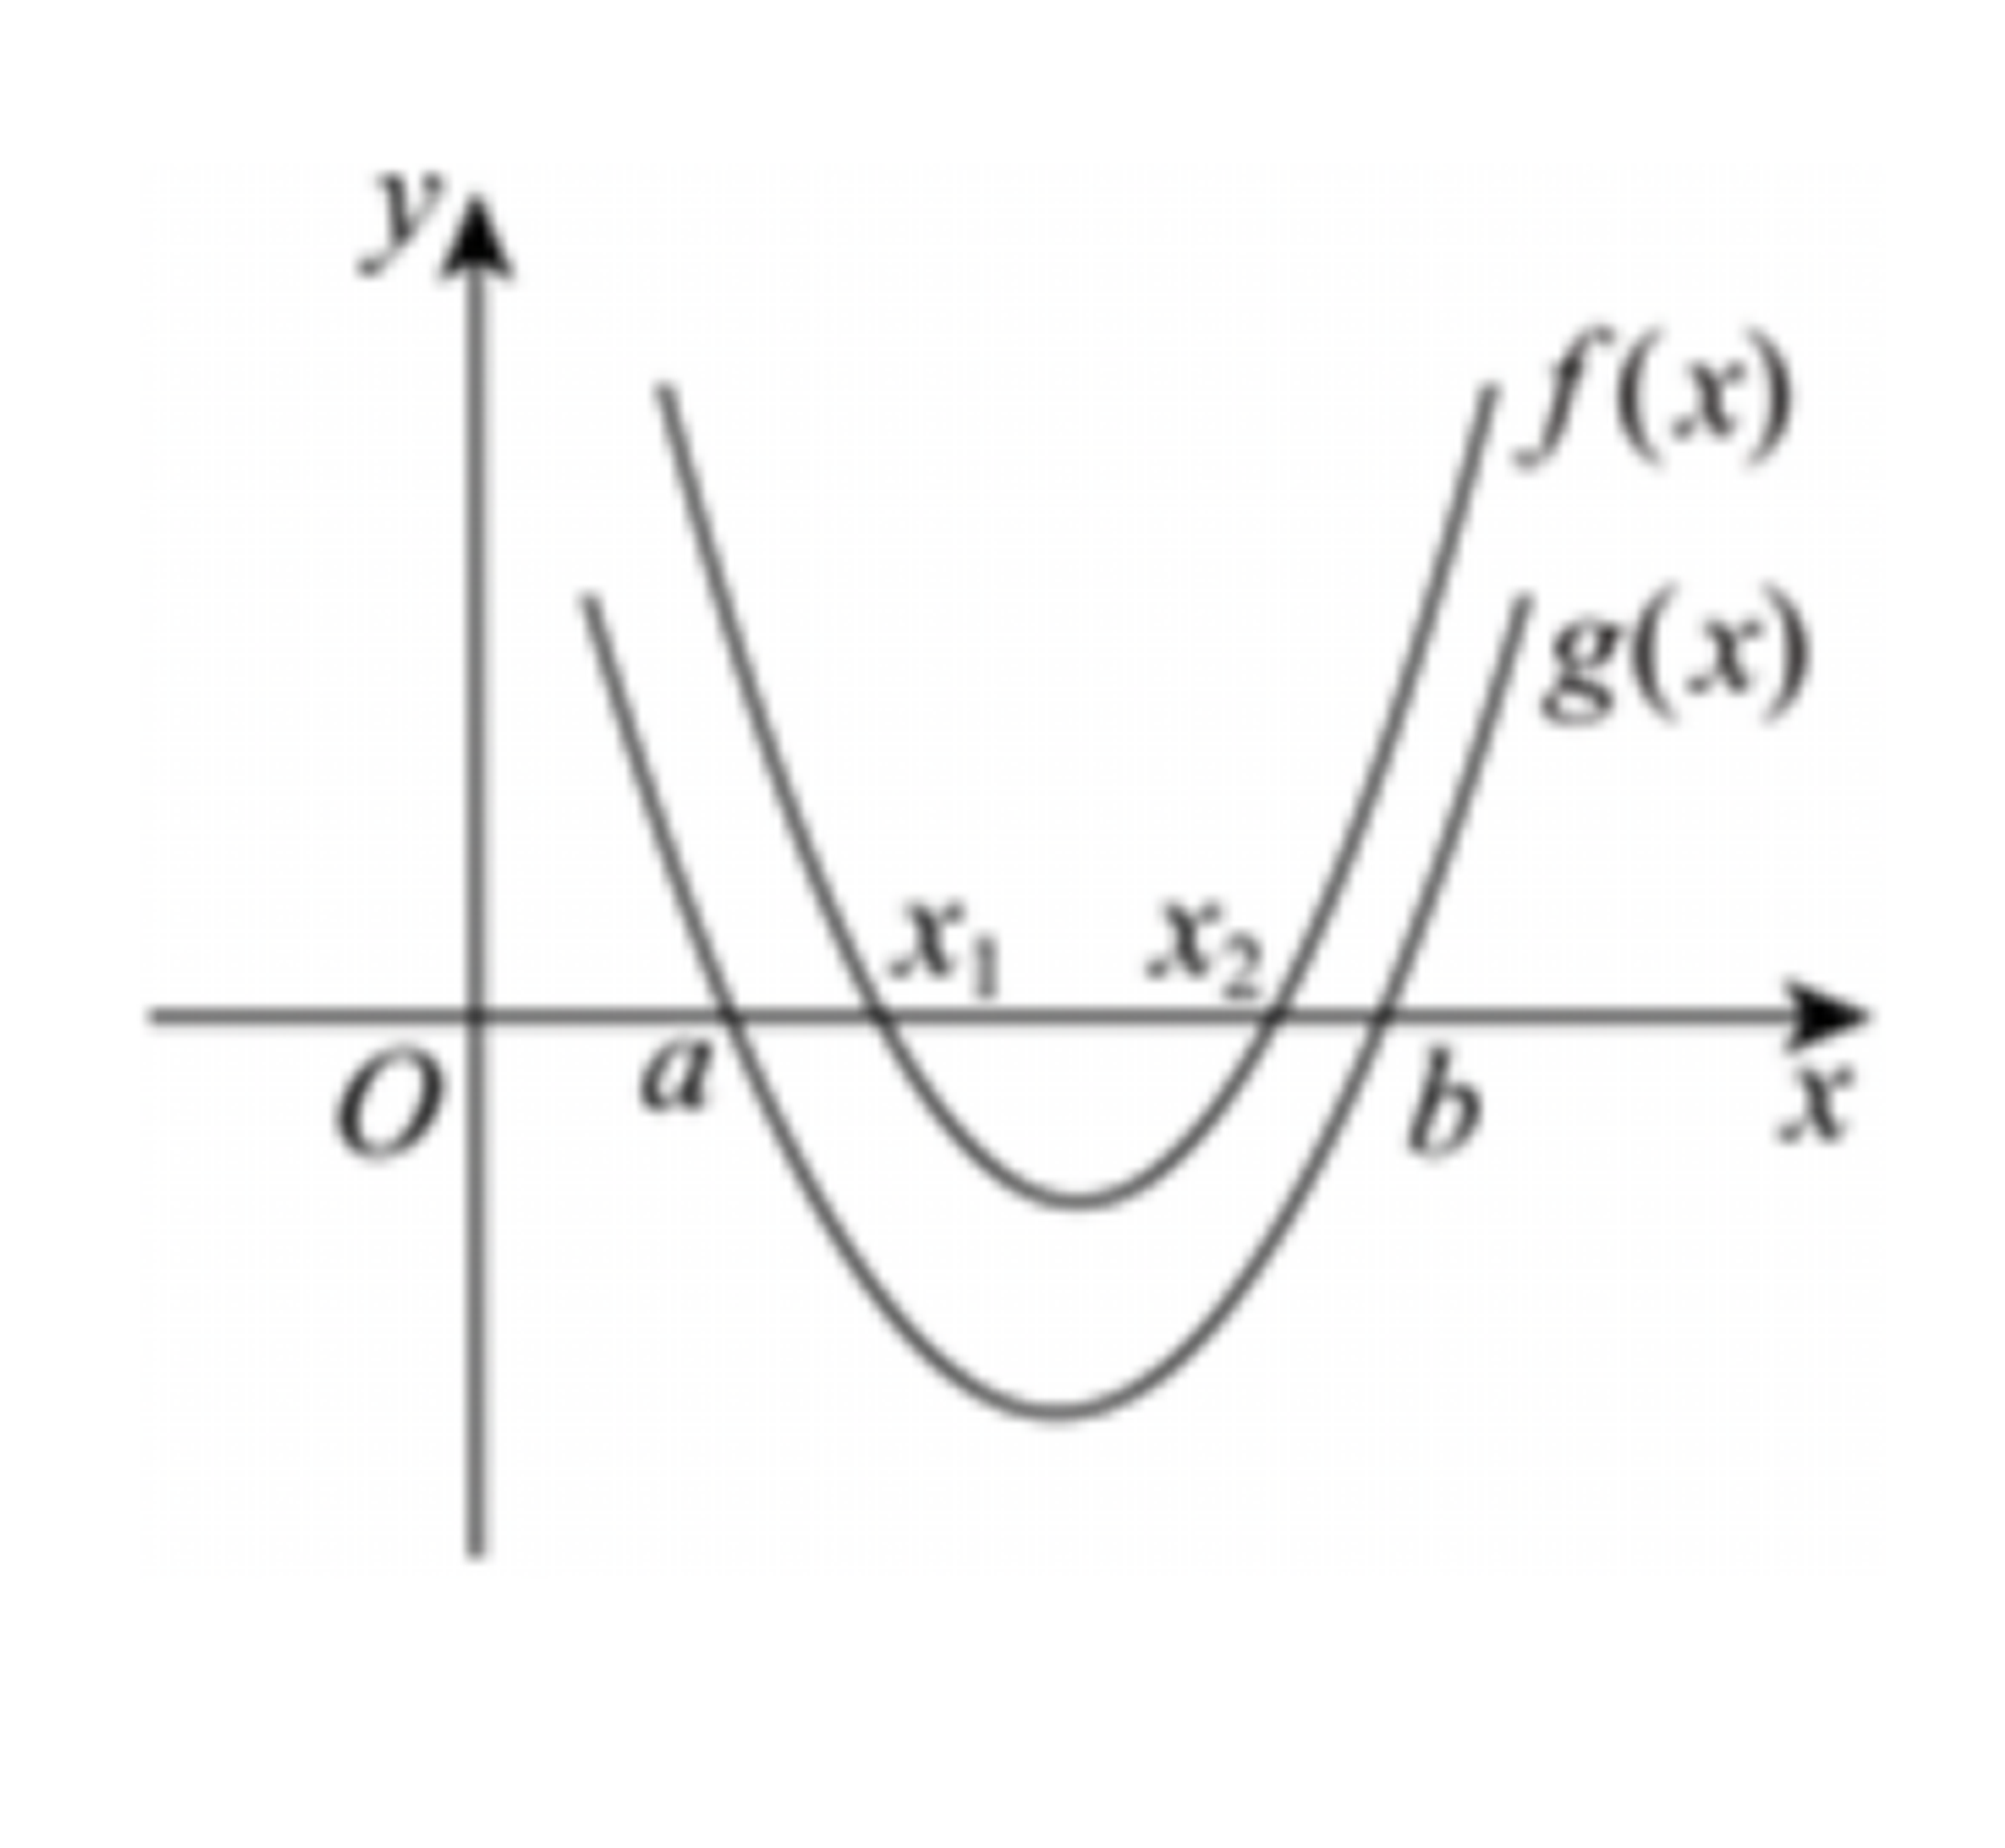
\includegraphics[width=0.30\textwidth]{figures/parabola_f_g_x1x2_h65.png}
\end{center}
\step{由图像得 $a<x_1<x_2<b$，故选 $B$.}
\solend
\fi

\end{enumerate}

\bigsec{三、解答题}

\begin{enumerate}
\setcounter{enumi}{16}

\item 已知 $a>0$，$b>0$，若 $a+b>4$，求证：$\dfrac a{b+2}$ 和 $\dfrac b{a+2}$ 中至少有一个大于 $\dfrac12$.

\ifanswer
\solbegin
\step{假设 $\dfrac a{b+2}\leqslant\dfrac12$，$\dfrac b{a+2}\leqslant\dfrac12$，}
\step{$a>0$，$b>0$，则 $a+2>0$，$b+2>0$，故 $2a\leqslant b+2$，$2b\leqslant a+2$，}
\step{两式相加得 $a+b\leqslant4$，与 $a+b>4$ 矛盾，故 $\dfrac a{b+2}$ 和 $\dfrac b{a+2}$ 中至少有一个大于 $\dfrac12$.}
\solend
\fi

\ansspace[6]

\item 已知集合 $A=\{x\mid-4<x<5\}$，$B=\{x\mid x\leqslant a-6\text{ 或 }x\geqslant a+2\}$.

\begin{enumerate}[label=(\arabic*)]

\item 若 $A\cup B=\R$，求实数 $a$ 的取值范围；

\item 若“$x\in A$”是“$x\in B$”的充分不必要条件，求实数 $a$ 的取值范围.

\end{enumerate}

\ifanswer
\solbegin
\stepm{(1)}{集合 $A=\{x\mid-4<x<5\}$，$B=\{x\mid x\leqslant a-6\text{ 或 }x\geqslant a+2\}$.}
\step{由 $A\cup B=\R$ 得 $\begin{cases}a-6\geqslant-4\\ a+2\leqslant5\end{cases}$，解得 $2\leqslant a\leqslant3$，$a$ 的取值范围为 $[2,3]$；}
\stepm{(2)}{若“$x\in A$”是“$x\in B$”的充分不必要条件，则 $A\subset B$，}
\step{则 $5\leqslant a-6$ 或 $-4\geqslant a+2$，解得 $a\leqslant-6$ 或 $a\geqslant11$.}
\solend
\fi

\ansspace[8]

% 注：原卷题干把命题 $P$ 印作“$\exists3\notin A$”（多一个存在量词），而【解析】两处均作
%     “$3\notin A$”；照录未改，见文件头“原卷笔误/存疑”③。
\item 已知集合 $A=\left\{x\mid\dfrac{x-1}{x-m}<0\right\}$，集合 $B=\left\{x\mid\left|\dfrac{x-1}{x-3}\right|\geqslant1\right\}$，命题 $P$：“$\exists3\notin A$”，命题
$Q$：$A\cap B\neq\varnothing$.

\begin{enumerate}[label=(\arabic*)]

\item 若命题 $P$ 为真命题，求 $m$ 的取值范围；

\item 若命题 $P$ 和命题 $Q$ 至少有一个为假命题，求实数 $m$ 的取值范围.

\end{enumerate}

\ifanswer
\solbegin
\stepm{(1)}{$A=\left\{x\mid\dfrac{x-1}{x-m}<0\right\}=\{x\mid(x-1)(x-m)<0\}$，}
\step{若命题 $P$：“$3\notin A$”为真命题，则 $(3-1)(3-m)\geqslant0$，解得 $m\leqslant3$，}
\step{故实数 $m$ 的取值范围为 $(-\infty,3]$；}
\stepm{(2)}{$B=\left\{x\mid\left|\dfrac{x-1}{x-3}\right|\geqslant1\right\}$，由 $\left|\dfrac{x-1}{x-3}\right|\geqslant1$，得 $\begin{cases}|x-1|\geqslant|x-3|\\ x\neq3\end{cases}$，}
\step{等价于 $\begin{cases}(x-1)^2\geqslant(x-3)^2\\ x\neq3\end{cases}$，解得 $x\geqslant2$ 且 $x\neq3$，所以 $B=[2,3)\cup(3,+\infty)$，}
\step{因为 $A=\{x\mid(x-1)(x-m)<0\}$，}
\step{当 $m=1$ 时，$A=\varnothing$，不满足 $A\cap B\neq\varnothing$，}
\step{当 $m<1$ 时，$A=(m,1)$，不满足 $A\cap B\neq\varnothing$，}
\step{当 $m>1$ 时，$A=(1,m)$，要使 $A\cap B\neq\varnothing$，则 $m>2$，}
\step{则若命题 $Q$：“$A\cap B\neq\varnothing$”为真命题时，实数 $m$ 的取值范围为 $(2,+\infty)$，}
\step{当命题 $P$ 与命题 $Q$ 都是真命题时，则 $\begin{cases}m\leqslant3\\ m>2\end{cases}$，解得 $2<m\leqslant3$，}
\step{则命题 $P$ 和命题 $Q$ 至少有一个为假命题时，得 $m\leqslant2$ 或 $m>3$，}
\step{故实数 $m$ 的取值范围为 $(-\infty,2]\cup(3,+\infty)$.}
\solend
\fi

\ansspace[8]

\item 已知函数 $y=ax^2-(a+2)x+2$，$a\in\R$.

\begin{enumerate}[label=(\arabic*)]

\item $y<3-2x$ 恒成立，求实数 $a$ 的取值范围；

% 注：原卷末句作“求实数 $a$ 的取值”（疑脱“范围”二字），照录未改，
%     见文件头“原卷笔误/存疑”⑤。
\item 若存在 $m>0$ 使关于 $x$ 的方程 $ax^2-(a+2)|x|+2=m+\dfrac1m+1$ 有四个不同的实根，
求实数 $a$ 的取值.

\end{enumerate}

\ifanswer
\solbegin
\stepm{(1)}{由题意得 $ax^2-(a+2)x+2<3-2x$ 恒成立，}
\step{即 $ax^2-ax-1<0$ 恒成立，}
\step{当 $a=0$ 时，$-1<0$ 恒成立，符合题意，}
\step{当 $a\neq0$ 时，则 $\begin{cases}a<0\\ \triangle=a^2+4a<0\end{cases}$，得 $\begin{cases}a<0\\ -4<a<0\end{cases}$，得 $-4<a<0$，}
\step{综上，$a$ 的取值范围为 $(-4,0]$.}
\stepm{(2)}{当 $m>0$ 时，令 $t=m+\dfrac1m+1\geqslant2\sqrt{m\times\dfrac1m}+1=3$，}
\step{当且仅当 $m=1$ 时取等号，}
% 注：题干只给“函数 $y=ax^2-(a+2)x+2$”，全卷未设 $f$，此处 $f(|x|)$ 无定义；
%     照录未改，见文件头“原卷笔误/存疑”④。
\step{则关于 $x$ 的方程 $f(|x|)=t$ 可化为 $a|x|^2-(a+2)|x|+2-t=0$，}
\step{关于 $x$ 的方程为 $a|x|^2-(a+2)|x|+2-t=0$ 有四个不等的实数根，}
\step{即 $ax^2-(a+2)x+2-t=0$，有两个不同的实数正根，}
\step{则 $\begin{cases}\triangle=(a+2)^2-4a(2-t)>0\\ \dfrac{a+2}a>0\\ \dfrac{2-t}a>0\end{cases}$，解得 $a<-2$，}
\step{由（1）得存在 $t\in[3,+\infty)$ 使得不等式 $4at+(a+2)^2-8a>0$ 成立，}
\step{故 $4a\times3+(a+2)^2-8a>0$，即 $a^2+8a+4>0$，}
\step{解得 $a<-4-2\sqrt3$ 或 $a>-4+2\sqrt3$，}
\step{综上，$a<-4-2\sqrt3$，所以 $a$ 的取值范围为 $(-\infty,-4-2\sqrt3)$.}
\solend
\fi

\ansspace[8]

\item 若集合 $A=B_1\cup B_2\cup\cdots\cup B_n$，其中 $B_1$、$B_2$、$\cdots$、$B_n$ 为非空集合，
$B_i\cap B_j=\varnothing$($1\leqslant i<j\leqslant n$)，则称集合 $\{B_1,B_2,\cdots,B_n\}$ 为集合 $A$ 的一个 $n$ 划分.

\begin{enumerate}[label=(\arabic*)]

\item 写出集合 $A=\{1,2,3\}$ 的所有不同的 2 划分；

\item 设 $\{B_1,B_2\}$ 为有理数集 $\Q$ 的一个 2 划分，且满足对任意 $x\in B_1$，任意 $y\in B_2$，都有
$x<y$，判断命题“$B_1$ 中的元素存在最大值，$B_2$ 中的元素存在最小值.”的真假，并说明
理由.

\item 设集合 $A=\{1,2,3,\cdots,16\}$，对于集合 $A$ 的任意一个 3 划分 $\{B_1,B_2,B_3\}$，判断是否存
在 $i\in\{1,2,3\}$，存在 $a$、$b\in B_i$，使得 $b-a\in B_i$ 成立，并说明理由.

\end{enumerate}

\ifanswer
\solbegin
% 注：原卷三个“2 划分”本有外层花括号（$\{\{1,2\},\{3\}\}$ 等），首轮误脱；
%     第二轮复核照原卷补回（原卷原样 / 本稿原错处：原脱外层花括号）。
\stepm{(1)}{集合 $A=\{1,2,3\}$ 的所有不同的 2 划分为 $\{\{1,2\},\{3\}\}$、$\{\{1,3\},\{2\}\}$、}
\step{$\{\{2,3\},\{1\}\}$.}
\stepm{(2)}{该命题为假命题，理由如下：}
\step{假设命题为真，则不妨设 $B_1$ 中元素的最大值为 $s$，$B_2$ 中元素的最小值为 $t$，}
\step{由题意得 $s<t$，所以 $s<\dfrac{s+t}2<t$，}
\step{因为 $s$ 为 $B_1$ 中元素的最大值，所以 $\dfrac{s+t}2\notin B_1$，}
\step{因为 $t$ 为 $B_2$ 中元素的最小值，所以 $\dfrac{s+t}2\notin B_2$，}
\step{因为 $B_1\cup B_2=\Q$，所以 $\dfrac{s+t}2\notin\Q$，}
\step{这与 $\dfrac{s+t}2\in\Q$ 矛盾，所以假设不成立，即命题不可能成立；}
\stepm{(3)}{由于集合 $A$ 中有 16 个元素，}
\step{所以 $B_1$、$B_2$、$B_3$ 中至少有一个集合至少包含 6 个元素，}
\step{不妨设 $B_1$ 中至少包含 6 个元素，}
\step{设 $b_1$、$b_2$、$b_3$、$b_4$、$b_5$、$b_6\in B_1$，且 $b_1<b_2<b_3<b_4<b_5<b_6$，}
\step{假设对任意 $i\in\{1,2,3\}$，对任意 $a$、$b\in B_i$，都有 $b-a\notin B_i$，}
\step{那么 $b_6-b_1$、$b_6-b_2$、$b_6-b_3$、$b_6-b_4$、$b_6-b_5\notin B_1$，}
\step{又因为 $b_6-b_1$、$b_6-b_2$、$b_6-b_3$、$b_6-b_4$、$b_6-b_5\in A$，}
\step{所以 $b_6-b_1$、$b_6-b_2$、$b_6-b_3$、$b_6-b_4$、$b_6-b_5\in B_2\cup B_3$，}
\step{则 $B_2$、$B_3$ 中必有一个集合}
\step{至少包含 $b_6-b_1$、$b_6-b_2$、$b_6-b_3$、$b_6-b_4$、$b_6-b_5$ 中的 3 个元素，}
\step{不妨设这 3 个元素为 $a_1$、$a_2$、$a_3\in B_2$，$a_1<a_2<a_3$，}
\step{由假设得 $a_3-a_1$、$a_3-a_2$、$a_2-a_1\notin B_2$，}
\step{对任意 $i$、$j$($1\leqslant j<i\leqslant3$)，存在 $m$、$n$($1\leqslant m<n\leqslant5$)，}
\step{都有 $a_i-a_j=b_6-b_m-b_6+b_n=b_n-b_m\notin B_1$，}
\step{又因为 $a_3-a_1$、$a_3-a_2$、$a_2-a_1\in B_3$，而 $a_3-a_1-(a_3-a_2)=a_2-a_1$，}
\step{与假设矛盾，所以假设不成立，}
\step{即存在 $i\in\{1,2,3\}$，存在 $a$、$b\in B_i$，使得 $b-a\in B_i$.}
\solend
\fi

\ansspace*[10]

\end{enumerate}

\end{document}
"
% 紧凑版：xelatex "\def\iscompact{1}% 高一65_大同中学_10月月考.tex
%   —— 高一上数学“2026-2027 年大同中学高一上 10 月月考”（讲评版）
% 试卷版：xelatex 高一65_大同中学_10月月考.tex
% 答案版：xelatex "\def\isanswer{1}% 高一65_大同中学_10月月考.tex
%   —— 高一上数学“2026-2027 年大同中学高一上 10 月月考”（讲评版）
% 试卷版：xelatex 高一65_大同中学_10月月考.tex
% 答案版：xelatex "\def\isanswer{1}\input{高一65_大同中学_10月月考.tex}"
% 紧凑版：xelatex "\def\iscompact{1}\input{高一65_大同中学_10月月考.tex}"
%
% 原始材料：微信公众号“魔都数学加油站”文章，作者破晓，连载“27学年高一65”；
% 原文标题“27学年高一65——2026-2027年上海市大同中学高一上10月月考”；
% 原文链接：https://mp.weixin.qq.com/s/h9ctuk-ByE1Vfg2Rx2C6bw。
% 页面标注发布时间 2026-10-17 21:58（上海）。
% 本次转录只据 `原图/高一65_大同中学_10月月考/` 的 11 张 PNG 逐页读图。
% 正文为 11 张 PNG 页（`01..11.png`）：
% 第 06、11 页 2560×3620，第 01、02、03、04、05、07、08、09、10 页 4762×6735
% （**同一篇各页分辨率不同**），均按页序读取。11 页全为试卷正文页（卷首标题在第 1 页页顶，
% 卷末解答题第 21 题解析止于第 11 页），无封面页、目录页、二维码或宣传页。
% 粉色斜排“魔都数学加油站”为卷面水印，与公众号页脚一并未录入。
%
% 卷首标题：照卷面印作“2026--2027 年大同中学高一上 10 月月考”，年份区间按全稿惯例排 en dash。
% 原卷只有一行标题、无副标题。
%
% 篇幅与题号：原卷自第 3 题起编号（第 1、2 题不在本卷内）。填空题 3—12（10 题）、
% 选择题 13—16（4 题）、解答题 17—21（5 题），共 19 题。本稿沿用原节与原题号，
% 只改排为全稿统一的大节样式（原卷小节标题为“一、填空题”“二、选择题”“三、解答题”）。
%
% 讲评版：原卷每题下直接印【答案】或【解析】。**只印【答案】的 4 题**（第 3、4、7、10 题），
% 本稿只给 \ans{}；其余 15 题都印【解析】（按全稿口径这类题不另提 \ans{}——第 12、13、14、
% 15、16 题的结论写在解析末句（“故选 B”“综上，n 的最大值为 14”等），亦照录在解析内）。
% 全卷无“答案印在题干括号内”的题（第 13—16 题的选择题括号内均空白）。
%
% 副标题：原卷未印副标题。本稿按“知识模块”口径标作“集合与常用逻辑用语、不等式”：
% 19 题中集合与常用逻辑用语 10 题（第 3、4、6、8、12、14、15、18、19、21 题），
% 不等式 9 题（含等式恒等、不等式性质、二次不等式、恒成立、基本不等式、不等式的证明：
% 第 5、7、9、10、11、13、16、17、20 题），两类均超过三分之一，故并标。口径同 高一63。
%
% 与原卷的排版差异：
%   ① 原卷每题下直接印【答案】/【解析】，本稿按全稿惯例将答案与解析置于答案版，试卷版保持干净；
%   ② 原卷未印副标题，本稿按“知识模块”口径补出；
%   ③ 原卷填空横线约四个字宽，本稿按全稿惯例统一排 \blankline[4.4em]；
%   ④ 原卷数集记号全为斜体：实数集作 $R$（第 6 题两处、第 8 题两处、第 15 题解析、第 18 题、
%      第 20 题题干），自然数集作 $N$（第 12 题题干“$n\in N,n\geqslant1$”），有理数集作 $Q$
%      （第 21 题 (2) 题干与解析共 4 处），本稿按全稿惯例统一改用 $\R$、$\N$、$\Q$
%      （同 高一63 排版差异④：记号归一）；空集记号原卷作 $\varnothing$，照录；
%   ⑤ 原卷用描述法时竖线排细竖“$|$”（如 $\{x|0<x<3\}$、$\{x|(x-1)(x-m)<0\}$），
%      本稿按全稿惯例排 \mid；
%   ⑥ 原卷判别式印作“$\triangle$”（第 8、14 题解析各 1 处、第 20 题解析 2 处，共 4 处），
%      本稿照录用 \triangle（同 高一39 成例），未改作 \Delta；
%   ⑦ 第 18—21 题的子问原卷各自另起一行、以“（1）”“（2）”标号，本稿按全稿惯例用
%      enumerate 的 (1)(2)(3)；解析中的子问标号一律用 \stepm{(1)}{…}；
%      第 18—21 题解析（原文以“（1）”“（2）”“（3）”冠于解析首句）同此；
%   ⑧ 选择题的作答括号原卷排半角“(　　)”（第 13—16 题括号内均空白），
%      本稿按全稿惯例排 \mbox{（\quad）}；选项字母后的句点照原卷排“A.”“B.”；
%   ⑨ 每道解答题原卷未留作答空白，本稿按全稿惯例加 \ansspace（末题用 \ansspace*）；
%   ⑩ 原卷在数学式内多处用半角逗号（如 $\{x|0<x<3\},B=\{x|x>2\}$、$m\in I_{14},k\in I_{14}$），
%      均照录未强改；句末句点按全稿惯例排西文句点。
%
% 原卷笔误/存疑（均照录未改，正文对应处另有 % 注）：
%   ① 第 13 题题干“下列不等式中一定成立是（　　）”脱一个“的”（当作“一定成立的是”），
%      8 倍放大确认非水印遮挡，本稿照录；
%   ② 第 15 题【解析】末段把题干条件“$x\geqslant10$”写成“$x\geqslant1$”
%      （“所以 $x+2+\frac{16}{x+2}(x\geqslant1)$ 的最小值不为 8”），与同段前面“令 $t=x+2$，
%      则 $t\geqslant12$”不合，本稿照录；
%   ③ 第 19 题题干把命题 $P$ 印作“$\exists3\notin A$”（多一个存在量词），而【解析】两处
%      均作“$3\notin A$”，前后记号不一，本稿照录；
%   ④ 第 20 题【解析】(2) 出现 $f(|x|)$，但题干只给“函数 $y=ax^2-(a+2)x+2$”、全卷未设 $f$，
%      本稿照录；
%   ⑤ 第 20 题 (2) 题干末句作“求实数 $a$ 的取值”（疑脱“范围”二字），本稿照录；
%   ⑥ 第 12 题【解析】第 18 步“它与 $P_n$ 中的任何其他数之和都不是整数”，该段所论为 $P_{14}$
%      （前后均作 $P_{14}$），此处 $P_n$ 疑当作 $P_{14}$，本稿照录。
%
% 第二轮复核（2026-10-18）订正「本稿抄错原卷」一处：
%   第 21 题 (1)【解析】原卷本作“$\{\{1,2\},\{3\}\}$、$\{\{1,3\},\{2\}\}$、$\{\{2,3\},\{1\}\}$”，
%   有外层花括号；首轮误脱外层花括号，并曾在文件头误记为“原卷未加外层花括号”（原第 ⑦ 条，
%   已撤销）。本次照原卷补回，正文对应处另有 % 注。
%
% 插图：第 16 题【解析】内有 1 幅图（两条开口向上的抛物线 $f(x)$、$g(x)$ 与 $x$ 轴交点
% 标 $a$、$x_1$、$x_2$、$b$，纵轴标 $y$、原点 $O$），解析第三行“画出函数 $g(x)$ 与函数 $f(x)$
% 的图像，如图所示”即指此图；取原卷截图（06.png，2560×3620）右半幅，4× LANCZOS 放大，
% 存 figures/parabola_f_g_x1x2_h65.png。该图在【解析】内，仅答案版出。
%
\documentclass[a4paper,11pt]{article}
\usepackage{common}

\begin{document}

\examtitlest[3]{2026--2027 年大同中学高一上 10 月月考}{集合与常用逻辑用语、不等式}

\bigsec{一、填空题}

\begin{enumerate}
\setcounter{enumi}{2}

\item 已知集合 $A=\{x\mid0<x<3\}$,$B=\{x\mid x>2\}$，则集合 $A\cup B=$\blankline[4.4em].

\ifanswer
\ans{$(0,+\infty)$}
\fi

\item “$x>1$ 或 $y>1$”的否定形式是\blankline[4.4em].

\ifanswer
\ans{$x\leqslant1$ 且 $y\leqslant1$}
\fi

\item 已知等式 $2x^2+3x+4=a(2x+1)(x+1)+b$ 恒成立，则常数 $a-b=$\blankline[4.4em].

\ifanswer
\solbegin
\step{因为等式 $2x^2+3x+4=a(2x+1)(x+1)+b$ 恒成立，}
\step{所以 $a(2x+1)(x+1)+b=2ax^2+3ax+a+b=2x^2+3x+4$，}
\step{所以 $\begin{cases}2a=2\\ 3a=3\\ a+b=4\end{cases}$，解得 $\begin{cases}a=1\\ b=3\end{cases}$，所以 $a-b=-2$.}
\solend
\fi

\item 全集为 $U=\R$，$A=\{x\mid|x|\geqslant2\}$，$B=\{y\mid y=x^2+1,x\in\R\}$，则 $A\cup\bar B=$\blankline[4.4em].

\ifanswer
\solbegin
\step{由题意得集合 $A=\{x\mid x\geqslant2\text{ 或 }x\leqslant-2\}$，}
\step{因为 $x^2+1\geqslant1$，所以集合 $B=\{x\mid x\geqslant1\}$，所以 $\bar B=\{x\mid x<1\}$，}
\step{则 $A\cup\bar B=\{x\mid x\geqslant2\text{ 或 }x<1\}$.}
\solend
\fi

\item 已知 $|x+3|+|x-5|=8$，则实数 $x$ 的取值范围为\blankline[4.4em].

\ifanswer
\ans{$[-3,5]$}
\fi

\item 已知集合 $A=\{x\in\R\mid ax^2+2x+1=0,a\in\R\}$ 只有一个元素，则 $a$ 的值为\blankline[4.4em].

\ifanswer
\solbegin
\step{当 $a=0$ 时，$A=\left\{-\dfrac12\right\}$；}
\step{当 $a\neq0$ 时，若集合 $A$ 只有一个元素，由 $\triangle=4-4a=0$ 得 $a=1$.}
\step{综上，当 $a=0$ 或 $a=1$ 时，集合 $A$ 只有一个元素.}
\solend
\fi

\item 已知不等式 $-x^2+bx+c>0$ 的解集为 $(3,4)$，则不等式 $cx^2+bx-1<0$ 的解集为\blankline[4.4em].

\ifanswer
\solbegin
\step{由题意得 3，4 是方程 $-x^2+bx+c=0$ 的两个实数根，}
\step{所以 $\begin{cases}3+4=b\\ 3\times4=-c\end{cases}$，得 $b=7$，$c=-12$，}
\step{则不等式 $cx^2+bx-1<0$，即为 $-12x^2+7x-1<0$，即 $12x^2-7x+1>0$，}
\step{化简得 $(3x-1)(4x-1)>0$，解得 $x<\dfrac14$ 或 $x>\dfrac13$，}
\step{即不等式 $cx^2+bx-1<0$ 的解集为 $\left(-\infty,\dfrac14\right)\cup\left(\dfrac13,+\infty\right)$.}
\solend
\fi

\item 对于区间 $(m,n)$，我们将 $n-m$ 的值称为该区间的长度. 若关于 $x$ 的不等式
$x^2+ax+a<0$ 有解，且解集的区间长度不超过 $2\sqrt3$，则实数 $a$ 的取值范围是\blankline[4.4em].

\ifanswer
\ans{$[-2,0)\cup(4,6]$}
\fi

\item 当 $x>0$ 时，关于 $x$ 的不等式 $(ax-1)(x^2+bx-4)\geqslant0$ 恒成立，则 $b+\dfrac2a$ 的最小值
为\blankline[4.4em].

\ifanswer
\solbegin
\step{由题意 $a\neq0$；}
\step{若 $a<0$，则 $x>0$ 时 $ax-1<0$ 恒成立，需 $x^2+bx-4\leqslant0$ 对一切 $x>0$ 成立，}
\step{而 $y=x^2+bx-4$ 的图象开口向上，当 $x$ 充分大时必为正值，矛盾，故 $a>0$.}
\step{当 $a>0$ 时，$ax-1=a\left(x-\dfrac1a\right)$，故原条件化为 $\left(x-\dfrac1a\right)(x^2+bx-4)\geqslant0$：}
\step{若 $0<x<\dfrac1a$，则 $x-\dfrac1a<0$，需 $x^2+bx-4\leqslant0$；}
\step{若 $x>\dfrac1a$，则 $x-\dfrac1a>0$，需 $x^2+bx-4\geqslant0$；}
\step{由 $y=x^2+bx-4$ 的连续性知 $x=\dfrac1a$ 是它的零点，}
\step{即 $\dfrac1{a^2}+\dfrac ba-4=0$，得 $b=4a-\dfrac1a$；}
\step{此时 $x^2+bx-4=x^2+\left(4a-\dfrac1a\right)x-4=(x+4a)\left(x-\dfrac1a\right)$，}
\step{由 $a>0$、$x>0$ 得 $x+4a>0$，}
\step{其符号与 $x-\dfrac1a$ 一致，故能与 $ax-1$ 同号，原不等式确在 $x>0$ 上恒成立.}
\step{于是 $b+\dfrac2a=4a-\dfrac1a+\dfrac2a=4a+\dfrac1a\geqslant2\sqrt{4a\cdot\dfrac1a}=4$，}
\step{当且仅当 $a=\dfrac12$ 时取等号，故最小值为 4.}
\solend
\fi

\item 设集合 $I_n=\{1,2,\cdots,n\}$，$n\in\N$，$n\geqslant1$，集合 $P_n=\left\{\dfrac m{\sqrt k}\mid m\in I_n,k\in I_n\right\}$，若 $P_n$ 的子集 $A$
中任意两个元素之和不是整数的平方，则称 $A$ 为“人文集”. 那么使 $P_n$ 能分成两个交集为空
集的“人文集”的并集，且这两个人文集的并集恰为 $P_n$ 时，$n$ 的最大值是\blankline[4.4em].

\ifanswer
\solbegin
\step{先证当 $n\geqslant15$ 时，$P_n$ 不能分成两个不相交的人文集的并集.}
\step{假设当 $n\geqslant15$ 时，$P_n$ 可以分成两个不相交的人文集的并集，}
\step{设 $A$ 和 $B$ 为两个不相交的人文集，使 $A\cup B=P_n\supseteq I_n$.}
\step{不妨设 $1\in A$，则由于 $1+3=2^2$，所以 $3\notin A$，即 $3\in B$.}
\step{同理可得，$6\in A$，$10\in B$. 又推出 $15\in A$，}
\step{但 $1+15=4^2$，这与 $A$ 为人文集相矛盾.}
\step{再证 $P_{14}$ 满足要求. 当 $k=1$ 时，$P_{14}=\left\{\dfrac m{\sqrt k}\mid m\in I_{14},k\in I_{14}\right\}$，}
\step{可以分成 2 个人文集的并集.}
\step{事实上，只要取 $A_1=\{1,2,4,6,9,11,13\}$，$B_1=\{3,5,7,8,10,12,14\}$，}
\step{则 $A_1$ 和 $B_1$ 都是人文集，且 $A_1\cup B_1=P_{14}$.}
\step{当 $k=4$ 时，集合 $\left\{\dfrac m{\sqrt k}\mid m\in I_{14}\right\}$ 中，除整数外，}
\step{剩下的数组成集合 $\left\{\dfrac12,\dfrac32,\dfrac52,\cdots,\dfrac{13}2\right\}$，}
\step{可以分为下列 2 个人文集的并：$A_2=\left\{\dfrac12,\dfrac52,\dfrac92,\dfrac{11}2\right\}$，$B_2=\left\{\dfrac32,\dfrac72,\dfrac{13}2\right\}$.}
\step{当 $k=9$ 时，集合 $\left\{\dfrac m{\sqrt k}\mid m\in I_{14}\right\}$ 中，除整数外，}
\step{剩下的数组成集合 $\left\{\dfrac13,\dfrac23,\dfrac43,\dfrac53,\cdots,\dfrac{13}3,\dfrac{14}3\right\}$，}
\step{可以分为下列 2 个人文集的并：$A_3=\left\{\dfrac13,\dfrac43,\dfrac53,\dfrac{10}3,\dfrac{13}3\right\}$，$B_3=\left\{\dfrac23,\dfrac73,\dfrac83,\dfrac{11}3,\dfrac{14}3\right\}$.}
\step{最后，集合 $C=\left\{\dfrac m{\sqrt k}\mid m\in I_{14},k\in I_{14},k\neq1,4,9\right\}$ 中的数的分母都是无理数，}
% 注：本行原卷作“$P_n$”，而该段所论为 $P_{14}$（前后均作 $P_{14}$），疑当作 $P_{14}$；
%     照录未改，见文件头“原卷笔误/存疑”⑥。
\step{它与 $P_n$ 中的任何其他数之和都不是整数，}
\step{因此，令 $A=A_1\cup A_2\cup A_3\cup C$，$B=B_1\cup B_2\cup B_3$，}
\step{则 $A$ 和 $B$ 是不相交的人文集，且 $A\cup B=P_{14}$.}
\step{综上，$n$ 的最大值为 14.}
\solend
\fi

\end{enumerate}

\bigsec{二、选择题}

\begin{enumerate}
\setcounter{enumi}{12}

% 注：原卷题干“下列不等式中一定成立是”脱一个“的”（当作“一定成立的是”），
%     照录未改，见文件头“原卷笔误/存疑”①。
\item 已知 $a>b$，下列不等式中一定成立是\mbox{（\quad）}

\keepwithprev
A. $a^2>b^2$\qquad B. $ac^2>bc^2$\qquad C. $\dfrac1a<\dfrac1b$\qquad D. $a+3>b-4$

\ifanswer
\solbegin
\step{对于 $A$，当 $a=-2$，$b=-4$ 时，不等式不成立，故 $A$ 错误；}
\step{对于 $B$，当 $c=0$ 时，不等式不成立，故 $B$ 错误；}
\step{对于 $C$，当 $a=2$，$b=-4$ 时，不等式不成立，故 $C$ 错误；}
\step{对于 $D$，因为 $a>b$，$3>-4$，必有 $a+3>b-4$ 成立，故 $D$ 正确.}
\step{故选 $D$.}
\solend
\fi

\item 已知 $a$ 为实数，那么“$|a|\leqslant2$”是“方程 $x^2+ax+1=0$ 没有实数解”的\mbox{（\quad）}

\keepwithprev
A. 充分而不必要条件\qquad B. 必要而不充分条件

C. 充要条件\qquad D. 既不充分也不必要条件

\ifanswer
\solbegin
\step{由方程 $x^2+ax+1=0$ 没有实数解，得 $\triangle=a^2-4<0$，则 $|a|<2$，}
\step{由 $|a|<2$ 得 $|a|\leqslant2$，反之不成立，}
\step{所以“$|a|\leqslant2$”是“方程 $x^2+ax+1=0$ 没有实数解”的必要而不充分条件.}
\step{故选 $B$.}
\solend
\fi

\item 下列命题为真命题的是\mbox{（\quad）}

\keepwithprev
A. $a>b>0$，当 $m>0$ 时，$\dfrac{a+m}{b+m}>\dfrac ab$

B. 集合 $A=\{x\mid y=x^2+1\}$ 与集合 $B=\{y\mid y=x^2+1\}$ 是相同的集合

C. 若 $b<a<0$，$m<0$，则 $\dfrac ma>\dfrac mb$

D. $x+2+\dfrac{16}{x+2}(x\geqslant10)$ 最小值为 8

\ifanswer
\solbegin
\step{对于 $A$，$\dfrac{a+m}{b+m}-\dfrac ab=\dfrac{b(a+m)-a(b+m)}{b(b+m)}=\dfrac{m(b-a)}{b(b+m)}$，}
\step{因为 $a>b>0$，$m>0$，所以 $b(b+m)>0$，$m(b-a)<0$，}
\step{所以 $\dfrac{a+m}{b+m}-\dfrac ab=\dfrac{m(b-a)}{b(b+m)}<0$，}
\step{即 $a>b>0$，当 $m>0$ 时，$\dfrac{a+m}{b+m}<\dfrac ab$，故 $A$ 错误；}
\step{对于 $B$，集合 $A=\{x\mid y=x^2+1\}=\R$，集合 $B=\{y\mid y=x^2+1\}=\{y\mid y\geqslant1\}$，}
\step{所以 $A\neq B$，故 $B$ 错误；}
\step{对于 $C$，$\dfrac ma-\dfrac mb=\dfrac{m(b-a)}{ab}$，}
\step{因为 $b<a<0$，$m<0$，所以 $ab>0$，$m(b-a)>0$，}
\step{所以 $\dfrac ma-\dfrac mb=\dfrac{m(b-a)}{ab}>0$，即 $\dfrac ma>\dfrac mb$，故 $C$ 正确；}
\step{对于 $D$，令 $t=x+2$，则 $t\geqslant12$，表达式变为 $t+\dfrac{16}t$，}
\step{$t+\dfrac{16}t\geqslant2\sqrt{t\cdot\dfrac{16}t}=8$，当且仅当 $t=4$ 时取等号，即等号不成立，}
% 注：原卷本行把题干条件“$x\geqslant10$”写成“$x\geqslant1$”，与同段“$t\geqslant12$”不合；
%     照录未改，见文件头“原卷笔误/存疑”②。
\step{所以 $x+2+\dfrac{16}{x+2}(x\geqslant1)$ 的最小值不为 8，故 $D$ 错误.}
\step{故选 $C$.}
\solend
\fi

\item 已知实数 $a<b$，关于 $x$ 的不等式 $x^2-(a+b)x+ab+\dfrac12<0$ 的解集为 $(x_1,x_2)$，则实数 $a$、
$b$、$x_1$、$x_2$ 从小到大的排列是\mbox{（\quad）}

\keepwithprev
A. $x_1<a<b<x_2$\qquad B. $a<x_1<x_2<b$\qquad C. $a<x_1<b<x_2$\qquad D. $x_1<a<x_2<b$

\ifanswer
\solbegin
\step{不等式 $x^2-(a+b)x+ab+\dfrac12<0$ 可化为 $(x-a)(x-b)+\dfrac12<0$，}
\step{设 $g(x)=(x-a)(x-b)$，$f(x)=g(x)+\dfrac12$，}
\step{画出函数 $g(x)$ 与函数 $f(x)$ 的图像，如图所示，}
% 图在【解析】内（仅答案版出），取原卷截图（06.png，2560×3620）右半幅，4× LANCZOS 放大。
\begin{center}
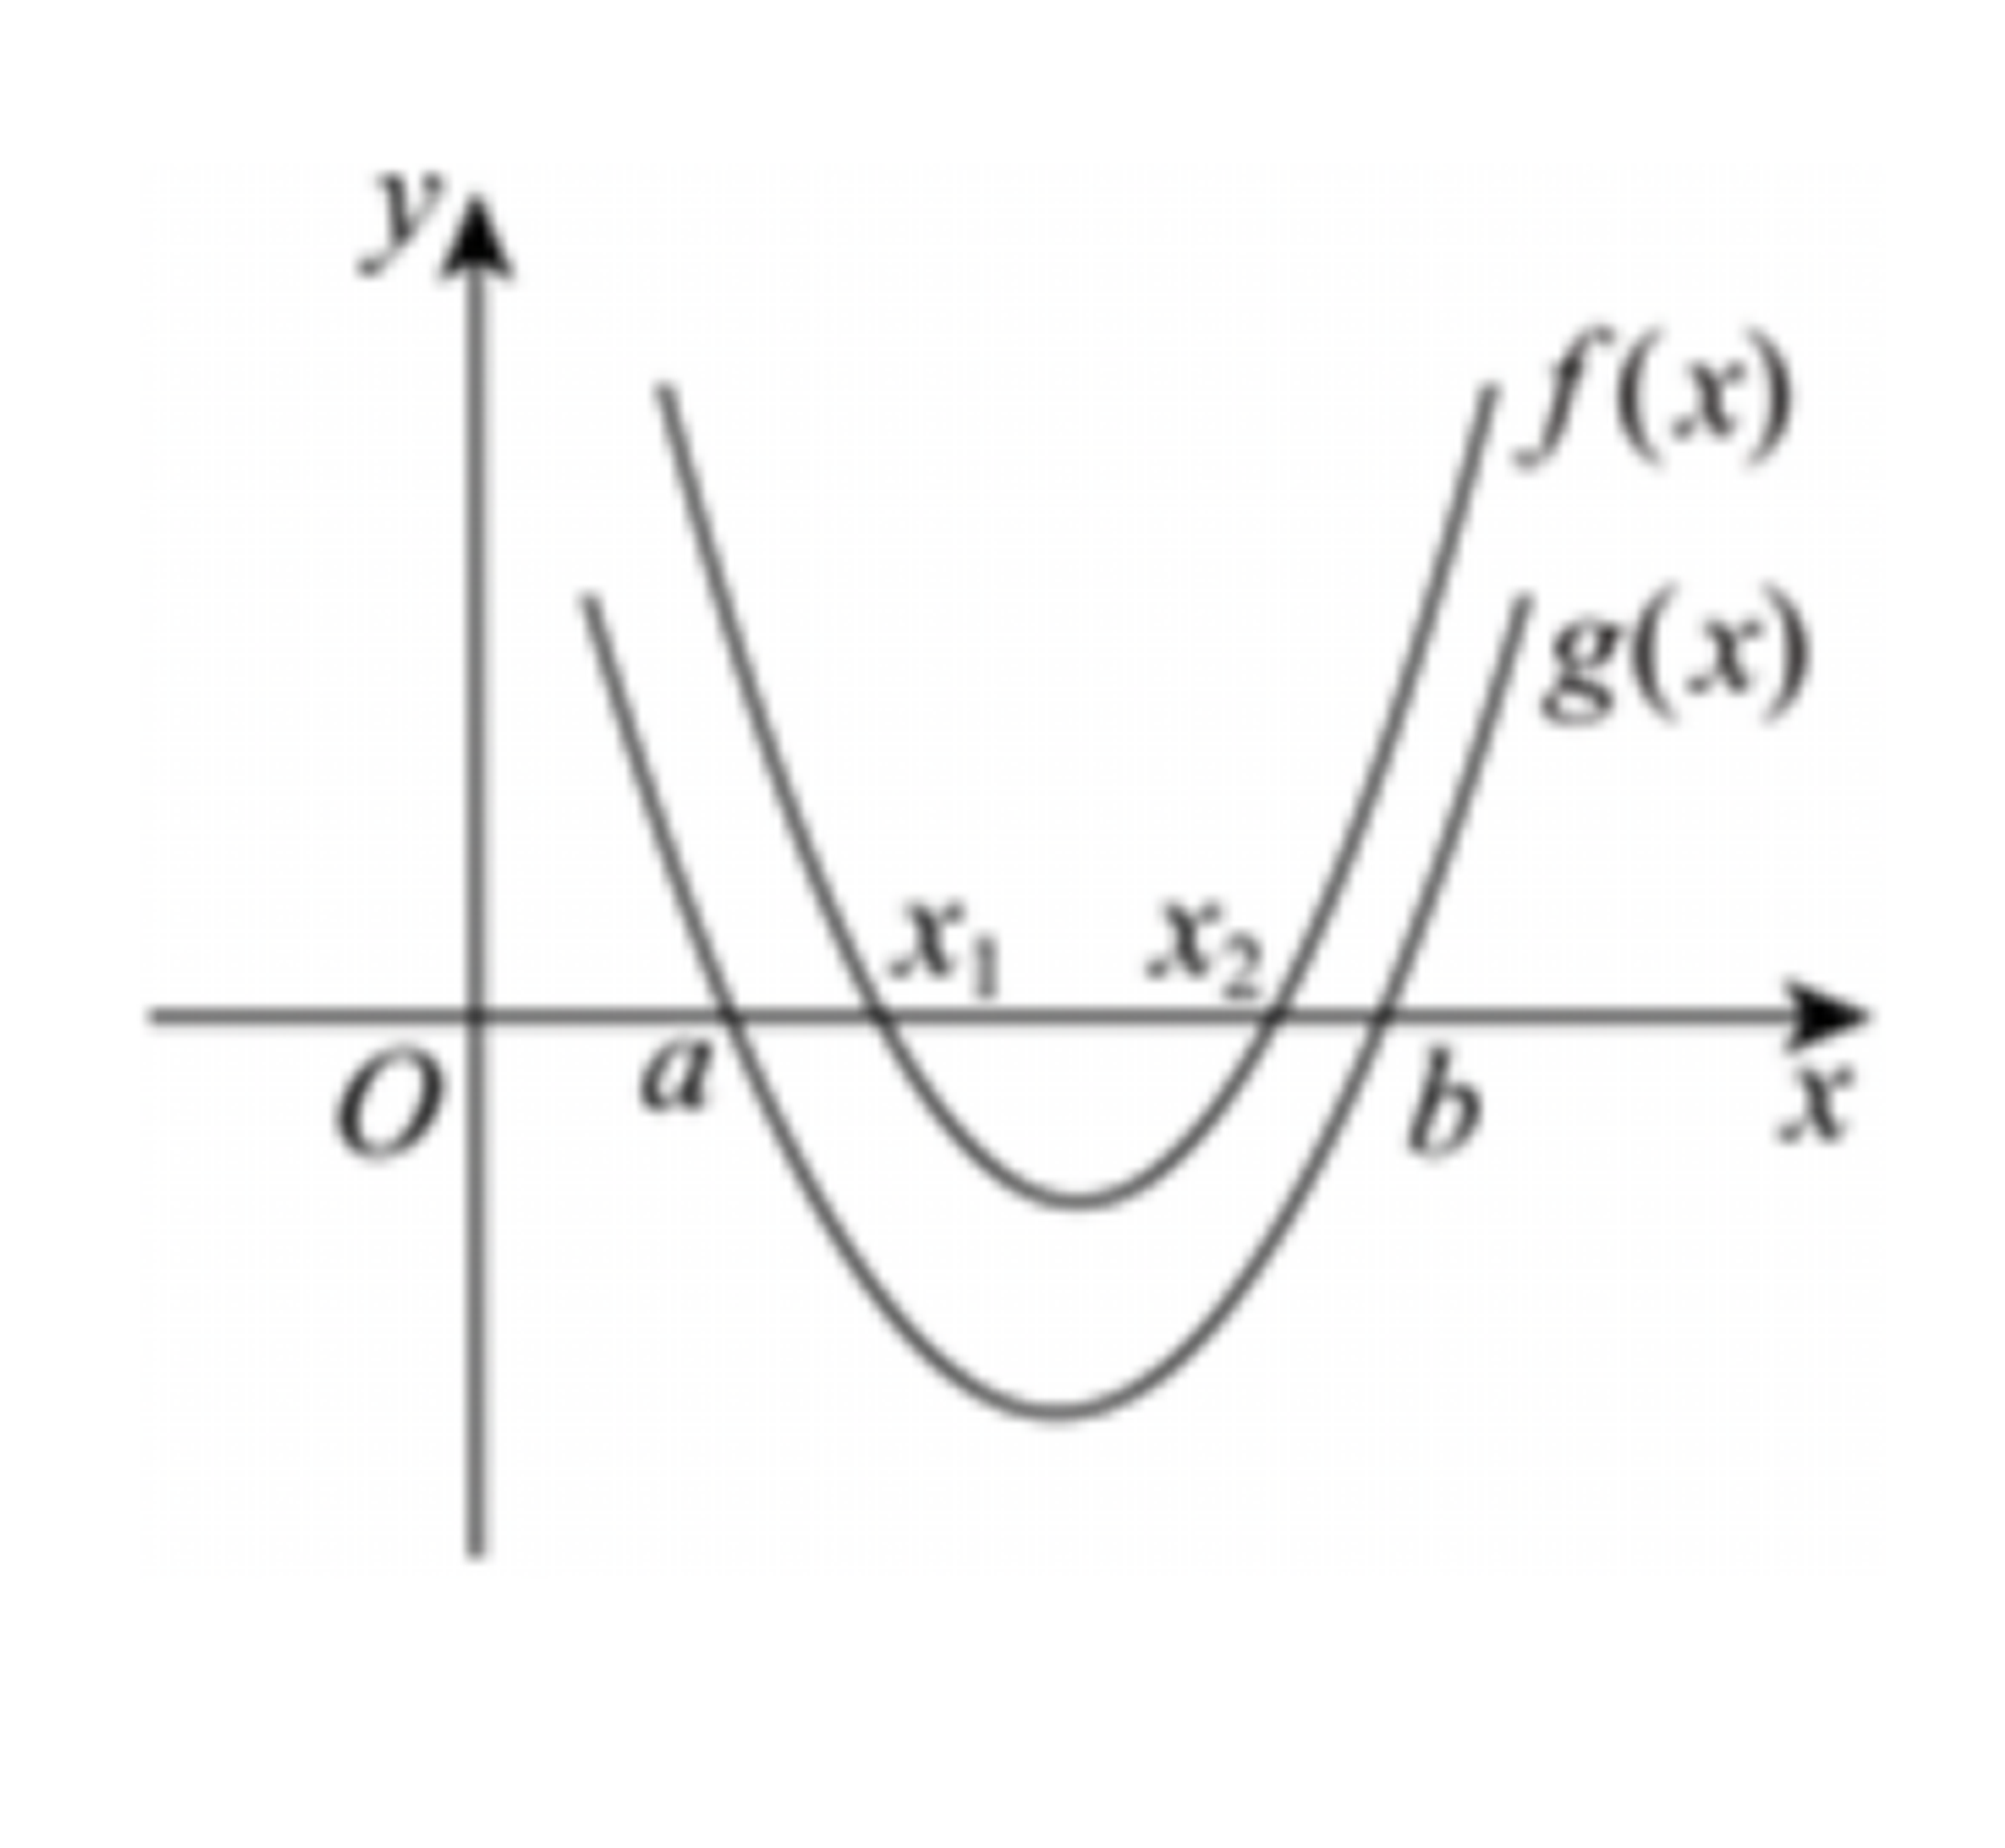
\includegraphics[width=0.30\textwidth]{figures/parabola_f_g_x1x2_h65.png}
\end{center}
\step{由图像得 $a<x_1<x_2<b$，故选 $B$.}
\solend
\fi

\end{enumerate}

\bigsec{三、解答题}

\begin{enumerate}
\setcounter{enumi}{16}

\item 已知 $a>0$，$b>0$，若 $a+b>4$，求证：$\dfrac a{b+2}$ 和 $\dfrac b{a+2}$ 中至少有一个大于 $\dfrac12$.

\ifanswer
\solbegin
\step{假设 $\dfrac a{b+2}\leqslant\dfrac12$，$\dfrac b{a+2}\leqslant\dfrac12$，}
\step{$a>0$，$b>0$，则 $a+2>0$，$b+2>0$，故 $2a\leqslant b+2$，$2b\leqslant a+2$，}
\step{两式相加得 $a+b\leqslant4$，与 $a+b>4$ 矛盾，故 $\dfrac a{b+2}$ 和 $\dfrac b{a+2}$ 中至少有一个大于 $\dfrac12$.}
\solend
\fi

\ansspace[6]

\item 已知集合 $A=\{x\mid-4<x<5\}$，$B=\{x\mid x\leqslant a-6\text{ 或 }x\geqslant a+2\}$.

\begin{enumerate}[label=(\arabic*)]

\item 若 $A\cup B=\R$，求实数 $a$ 的取值范围；

\item 若“$x\in A$”是“$x\in B$”的充分不必要条件，求实数 $a$ 的取值范围.

\end{enumerate}

\ifanswer
\solbegin
\stepm{(1)}{集合 $A=\{x\mid-4<x<5\}$，$B=\{x\mid x\leqslant a-6\text{ 或 }x\geqslant a+2\}$.}
\step{由 $A\cup B=\R$ 得 $\begin{cases}a-6\geqslant-4\\ a+2\leqslant5\end{cases}$，解得 $2\leqslant a\leqslant3$，$a$ 的取值范围为 $[2,3]$；}
\stepm{(2)}{若“$x\in A$”是“$x\in B$”的充分不必要条件，则 $A\subset B$，}
\step{则 $5\leqslant a-6$ 或 $-4\geqslant a+2$，解得 $a\leqslant-6$ 或 $a\geqslant11$.}
\solend
\fi

\ansspace[8]

% 注：原卷题干把命题 $P$ 印作“$\exists3\notin A$”（多一个存在量词），而【解析】两处均作
%     “$3\notin A$”；照录未改，见文件头“原卷笔误/存疑”③。
\item 已知集合 $A=\left\{x\mid\dfrac{x-1}{x-m}<0\right\}$，集合 $B=\left\{x\mid\left|\dfrac{x-1}{x-3}\right|\geqslant1\right\}$，命题 $P$：“$\exists3\notin A$”，命题
$Q$：$A\cap B\neq\varnothing$.

\begin{enumerate}[label=(\arabic*)]

\item 若命题 $P$ 为真命题，求 $m$ 的取值范围；

\item 若命题 $P$ 和命题 $Q$ 至少有一个为假命题，求实数 $m$ 的取值范围.

\end{enumerate}

\ifanswer
\solbegin
\stepm{(1)}{$A=\left\{x\mid\dfrac{x-1}{x-m}<0\right\}=\{x\mid(x-1)(x-m)<0\}$，}
\step{若命题 $P$：“$3\notin A$”为真命题，则 $(3-1)(3-m)\geqslant0$，解得 $m\leqslant3$，}
\step{故实数 $m$ 的取值范围为 $(-\infty,3]$；}
\stepm{(2)}{$B=\left\{x\mid\left|\dfrac{x-1}{x-3}\right|\geqslant1\right\}$，由 $\left|\dfrac{x-1}{x-3}\right|\geqslant1$，得 $\begin{cases}|x-1|\geqslant|x-3|\\ x\neq3\end{cases}$，}
\step{等价于 $\begin{cases}(x-1)^2\geqslant(x-3)^2\\ x\neq3\end{cases}$，解得 $x\geqslant2$ 且 $x\neq3$，所以 $B=[2,3)\cup(3,+\infty)$，}
\step{因为 $A=\{x\mid(x-1)(x-m)<0\}$，}
\step{当 $m=1$ 时，$A=\varnothing$，不满足 $A\cap B\neq\varnothing$，}
\step{当 $m<1$ 时，$A=(m,1)$，不满足 $A\cap B\neq\varnothing$，}
\step{当 $m>1$ 时，$A=(1,m)$，要使 $A\cap B\neq\varnothing$，则 $m>2$，}
\step{则若命题 $Q$：“$A\cap B\neq\varnothing$”为真命题时，实数 $m$ 的取值范围为 $(2,+\infty)$，}
\step{当命题 $P$ 与命题 $Q$ 都是真命题时，则 $\begin{cases}m\leqslant3\\ m>2\end{cases}$，解得 $2<m\leqslant3$，}
\step{则命题 $P$ 和命题 $Q$ 至少有一个为假命题时，得 $m\leqslant2$ 或 $m>3$，}
\step{故实数 $m$ 的取值范围为 $(-\infty,2]\cup(3,+\infty)$.}
\solend
\fi

\ansspace[8]

\item 已知函数 $y=ax^2-(a+2)x+2$，$a\in\R$.

\begin{enumerate}[label=(\arabic*)]

\item $y<3-2x$ 恒成立，求实数 $a$ 的取值范围；

% 注：原卷末句作“求实数 $a$ 的取值”（疑脱“范围”二字），照录未改，
%     见文件头“原卷笔误/存疑”⑤。
\item 若存在 $m>0$ 使关于 $x$ 的方程 $ax^2-(a+2)|x|+2=m+\dfrac1m+1$ 有四个不同的实根，
求实数 $a$ 的取值.

\end{enumerate}

\ifanswer
\solbegin
\stepm{(1)}{由题意得 $ax^2-(a+2)x+2<3-2x$ 恒成立，}
\step{即 $ax^2-ax-1<0$ 恒成立，}
\step{当 $a=0$ 时，$-1<0$ 恒成立，符合题意，}
\step{当 $a\neq0$ 时，则 $\begin{cases}a<0\\ \triangle=a^2+4a<0\end{cases}$，得 $\begin{cases}a<0\\ -4<a<0\end{cases}$，得 $-4<a<0$，}
\step{综上，$a$ 的取值范围为 $(-4,0]$.}
\stepm{(2)}{当 $m>0$ 时，令 $t=m+\dfrac1m+1\geqslant2\sqrt{m\times\dfrac1m}+1=3$，}
\step{当且仅当 $m=1$ 时取等号，}
% 注：题干只给“函数 $y=ax^2-(a+2)x+2$”，全卷未设 $f$，此处 $f(|x|)$ 无定义；
%     照录未改，见文件头“原卷笔误/存疑”④。
\step{则关于 $x$ 的方程 $f(|x|)=t$ 可化为 $a|x|^2-(a+2)|x|+2-t=0$，}
\step{关于 $x$ 的方程为 $a|x|^2-(a+2)|x|+2-t=0$ 有四个不等的实数根，}
\step{即 $ax^2-(a+2)x+2-t=0$，有两个不同的实数正根，}
\step{则 $\begin{cases}\triangle=(a+2)^2-4a(2-t)>0\\ \dfrac{a+2}a>0\\ \dfrac{2-t}a>0\end{cases}$，解得 $a<-2$，}
\step{由（1）得存在 $t\in[3,+\infty)$ 使得不等式 $4at+(a+2)^2-8a>0$ 成立，}
\step{故 $4a\times3+(a+2)^2-8a>0$，即 $a^2+8a+4>0$，}
\step{解得 $a<-4-2\sqrt3$ 或 $a>-4+2\sqrt3$，}
\step{综上，$a<-4-2\sqrt3$，所以 $a$ 的取值范围为 $(-\infty,-4-2\sqrt3)$.}
\solend
\fi

\ansspace[8]

\item 若集合 $A=B_1\cup B_2\cup\cdots\cup B_n$，其中 $B_1$、$B_2$、$\cdots$、$B_n$ 为非空集合，
$B_i\cap B_j=\varnothing$($1\leqslant i<j\leqslant n$)，则称集合 $\{B_1,B_2,\cdots,B_n\}$ 为集合 $A$ 的一个 $n$ 划分.

\begin{enumerate}[label=(\arabic*)]

\item 写出集合 $A=\{1,2,3\}$ 的所有不同的 2 划分；

\item 设 $\{B_1,B_2\}$ 为有理数集 $\Q$ 的一个 2 划分，且满足对任意 $x\in B_1$，任意 $y\in B_2$，都有
$x<y$，判断命题“$B_1$ 中的元素存在最大值，$B_2$ 中的元素存在最小值.”的真假，并说明
理由.

\item 设集合 $A=\{1,2,3,\cdots,16\}$，对于集合 $A$ 的任意一个 3 划分 $\{B_1,B_2,B_3\}$，判断是否存
在 $i\in\{1,2,3\}$，存在 $a$、$b\in B_i$，使得 $b-a\in B_i$ 成立，并说明理由.

\end{enumerate}

\ifanswer
\solbegin
% 注：原卷三个“2 划分”本有外层花括号（$\{\{1,2\},\{3\}\}$ 等），首轮误脱；
%     第二轮复核照原卷补回（原卷原样 / 本稿原错处：原脱外层花括号）。
\stepm{(1)}{集合 $A=\{1,2,3\}$ 的所有不同的 2 划分为 $\{\{1,2\},\{3\}\}$、$\{\{1,3\},\{2\}\}$、}
\step{$\{\{2,3\},\{1\}\}$.}
\stepm{(2)}{该命题为假命题，理由如下：}
\step{假设命题为真，则不妨设 $B_1$ 中元素的最大值为 $s$，$B_2$ 中元素的最小值为 $t$，}
\step{由题意得 $s<t$，所以 $s<\dfrac{s+t}2<t$，}
\step{因为 $s$ 为 $B_1$ 中元素的最大值，所以 $\dfrac{s+t}2\notin B_1$，}
\step{因为 $t$ 为 $B_2$ 中元素的最小值，所以 $\dfrac{s+t}2\notin B_2$，}
\step{因为 $B_1\cup B_2=\Q$，所以 $\dfrac{s+t}2\notin\Q$，}
\step{这与 $\dfrac{s+t}2\in\Q$ 矛盾，所以假设不成立，即命题不可能成立；}
\stepm{(3)}{由于集合 $A$ 中有 16 个元素，}
\step{所以 $B_1$、$B_2$、$B_3$ 中至少有一个集合至少包含 6 个元素，}
\step{不妨设 $B_1$ 中至少包含 6 个元素，}
\step{设 $b_1$、$b_2$、$b_3$、$b_4$、$b_5$、$b_6\in B_1$，且 $b_1<b_2<b_3<b_4<b_5<b_6$，}
\step{假设对任意 $i\in\{1,2,3\}$，对任意 $a$、$b\in B_i$，都有 $b-a\notin B_i$，}
\step{那么 $b_6-b_1$、$b_6-b_2$、$b_6-b_3$、$b_6-b_4$、$b_6-b_5\notin B_1$，}
\step{又因为 $b_6-b_1$、$b_6-b_2$、$b_6-b_3$、$b_6-b_4$、$b_6-b_5\in A$，}
\step{所以 $b_6-b_1$、$b_6-b_2$、$b_6-b_3$、$b_6-b_4$、$b_6-b_5\in B_2\cup B_3$，}
\step{则 $B_2$、$B_3$ 中必有一个集合}
\step{至少包含 $b_6-b_1$、$b_6-b_2$、$b_6-b_3$、$b_6-b_4$、$b_6-b_5$ 中的 3 个元素，}
\step{不妨设这 3 个元素为 $a_1$、$a_2$、$a_3\in B_2$，$a_1<a_2<a_3$，}
\step{由假设得 $a_3-a_1$、$a_3-a_2$、$a_2-a_1\notin B_2$，}
\step{对任意 $i$、$j$($1\leqslant j<i\leqslant3$)，存在 $m$、$n$($1\leqslant m<n\leqslant5$)，}
\step{都有 $a_i-a_j=b_6-b_m-b_6+b_n=b_n-b_m\notin B_1$，}
\step{又因为 $a_3-a_1$、$a_3-a_2$、$a_2-a_1\in B_3$，而 $a_3-a_1-(a_3-a_2)=a_2-a_1$，}
\step{与假设矛盾，所以假设不成立，}
\step{即存在 $i\in\{1,2,3\}$，存在 $a$、$b\in B_i$，使得 $b-a\in B_i$.}
\solend
\fi

\ansspace*[10]

\end{enumerate}

\end{document}
"
% 紧凑版：xelatex "\def\iscompact{1}% 高一65_大同中学_10月月考.tex
%   —— 高一上数学“2026-2027 年大同中学高一上 10 月月考”（讲评版）
% 试卷版：xelatex 高一65_大同中学_10月月考.tex
% 答案版：xelatex "\def\isanswer{1}\input{高一65_大同中学_10月月考.tex}"
% 紧凑版：xelatex "\def\iscompact{1}\input{高一65_大同中学_10月月考.tex}"
%
% 原始材料：微信公众号“魔都数学加油站”文章，作者破晓，连载“27学年高一65”；
% 原文标题“27学年高一65——2026-2027年上海市大同中学高一上10月月考”；
% 原文链接：https://mp.weixin.qq.com/s/h9ctuk-ByE1Vfg2Rx2C6bw。
% 页面标注发布时间 2026-10-17 21:58（上海）。
% 本次转录只据 `原图/高一65_大同中学_10月月考/` 的 11 张 PNG 逐页读图。
% 正文为 11 张 PNG 页（`01..11.png`）：
% 第 06、11 页 2560×3620，第 01、02、03、04、05、07、08、09、10 页 4762×6735
% （**同一篇各页分辨率不同**），均按页序读取。11 页全为试卷正文页（卷首标题在第 1 页页顶，
% 卷末解答题第 21 题解析止于第 11 页），无封面页、目录页、二维码或宣传页。
% 粉色斜排“魔都数学加油站”为卷面水印，与公众号页脚一并未录入。
%
% 卷首标题：照卷面印作“2026--2027 年大同中学高一上 10 月月考”，年份区间按全稿惯例排 en dash。
% 原卷只有一行标题、无副标题。
%
% 篇幅与题号：原卷自第 3 题起编号（第 1、2 题不在本卷内）。填空题 3—12（10 题）、
% 选择题 13—16（4 题）、解答题 17—21（5 题），共 19 题。本稿沿用原节与原题号，
% 只改排为全稿统一的大节样式（原卷小节标题为“一、填空题”“二、选择题”“三、解答题”）。
%
% 讲评版：原卷每题下直接印【答案】或【解析】。**只印【答案】的 4 题**（第 3、4、7、10 题），
% 本稿只给 \ans{}；其余 15 题都印【解析】（按全稿口径这类题不另提 \ans{}——第 12、13、14、
% 15、16 题的结论写在解析末句（“故选 B”“综上，n 的最大值为 14”等），亦照录在解析内）。
% 全卷无“答案印在题干括号内”的题（第 13—16 题的选择题括号内均空白）。
%
% 副标题：原卷未印副标题。本稿按“知识模块”口径标作“集合与常用逻辑用语、不等式”：
% 19 题中集合与常用逻辑用语 10 题（第 3、4、6、8、12、14、15、18、19、21 题），
% 不等式 9 题（含等式恒等、不等式性质、二次不等式、恒成立、基本不等式、不等式的证明：
% 第 5、7、9、10、11、13、16、17、20 题），两类均超过三分之一，故并标。口径同 高一63。
%
% 与原卷的排版差异：
%   ① 原卷每题下直接印【答案】/【解析】，本稿按全稿惯例将答案与解析置于答案版，试卷版保持干净；
%   ② 原卷未印副标题，本稿按“知识模块”口径补出；
%   ③ 原卷填空横线约四个字宽，本稿按全稿惯例统一排 \blankline[4.4em]；
%   ④ 原卷数集记号全为斜体：实数集作 $R$（第 6 题两处、第 8 题两处、第 15 题解析、第 18 题、
%      第 20 题题干），自然数集作 $N$（第 12 题题干“$n\in N,n\geqslant1$”），有理数集作 $Q$
%      （第 21 题 (2) 题干与解析共 4 处），本稿按全稿惯例统一改用 $\R$、$\N$、$\Q$
%      （同 高一63 排版差异④：记号归一）；空集记号原卷作 $\varnothing$，照录；
%   ⑤ 原卷用描述法时竖线排细竖“$|$”（如 $\{x|0<x<3\}$、$\{x|(x-1)(x-m)<0\}$），
%      本稿按全稿惯例排 \mid；
%   ⑥ 原卷判别式印作“$\triangle$”（第 8、14 题解析各 1 处、第 20 题解析 2 处，共 4 处），
%      本稿照录用 \triangle（同 高一39 成例），未改作 \Delta；
%   ⑦ 第 18—21 题的子问原卷各自另起一行、以“（1）”“（2）”标号，本稿按全稿惯例用
%      enumerate 的 (1)(2)(3)；解析中的子问标号一律用 \stepm{(1)}{…}；
%      第 18—21 题解析（原文以“（1）”“（2）”“（3）”冠于解析首句）同此；
%   ⑧ 选择题的作答括号原卷排半角“(　　)”（第 13—16 题括号内均空白），
%      本稿按全稿惯例排 \mbox{（\quad）}；选项字母后的句点照原卷排“A.”“B.”；
%   ⑨ 每道解答题原卷未留作答空白，本稿按全稿惯例加 \ansspace（末题用 \ansspace*）；
%   ⑩ 原卷在数学式内多处用半角逗号（如 $\{x|0<x<3\},B=\{x|x>2\}$、$m\in I_{14},k\in I_{14}$），
%      均照录未强改；句末句点按全稿惯例排西文句点。
%
% 原卷笔误/存疑（均照录未改，正文对应处另有 % 注）：
%   ① 第 13 题题干“下列不等式中一定成立是（　　）”脱一个“的”（当作“一定成立的是”），
%      8 倍放大确认非水印遮挡，本稿照录；
%   ② 第 15 题【解析】末段把题干条件“$x\geqslant10$”写成“$x\geqslant1$”
%      （“所以 $x+2+\frac{16}{x+2}(x\geqslant1)$ 的最小值不为 8”），与同段前面“令 $t=x+2$，
%      则 $t\geqslant12$”不合，本稿照录；
%   ③ 第 19 题题干把命题 $P$ 印作“$\exists3\notin A$”（多一个存在量词），而【解析】两处
%      均作“$3\notin A$”，前后记号不一，本稿照录；
%   ④ 第 20 题【解析】(2) 出现 $f(|x|)$，但题干只给“函数 $y=ax^2-(a+2)x+2$”、全卷未设 $f$，
%      本稿照录；
%   ⑤ 第 20 题 (2) 题干末句作“求实数 $a$ 的取值”（疑脱“范围”二字），本稿照录；
%   ⑥ 第 12 题【解析】第 18 步“它与 $P_n$ 中的任何其他数之和都不是整数”，该段所论为 $P_{14}$
%      （前后均作 $P_{14}$），此处 $P_n$ 疑当作 $P_{14}$，本稿照录。
%
% 第二轮复核（2026-10-18）订正「本稿抄错原卷」一处：
%   第 21 题 (1)【解析】原卷本作“$\{\{1,2\},\{3\}\}$、$\{\{1,3\},\{2\}\}$、$\{\{2,3\},\{1\}\}$”，
%   有外层花括号；首轮误脱外层花括号，并曾在文件头误记为“原卷未加外层花括号”（原第 ⑦ 条，
%   已撤销）。本次照原卷补回，正文对应处另有 % 注。
%
% 插图：第 16 题【解析】内有 1 幅图（两条开口向上的抛物线 $f(x)$、$g(x)$ 与 $x$ 轴交点
% 标 $a$、$x_1$、$x_2$、$b$，纵轴标 $y$、原点 $O$），解析第三行“画出函数 $g(x)$ 与函数 $f(x)$
% 的图像，如图所示”即指此图；取原卷截图（06.png，2560×3620）右半幅，4× LANCZOS 放大，
% 存 figures/parabola_f_g_x1x2_h65.png。该图在【解析】内，仅答案版出。
%
\documentclass[a4paper,11pt]{article}
\usepackage{common}

\begin{document}

\examtitlest[3]{2026--2027 年大同中学高一上 10 月月考}{集合与常用逻辑用语、不等式}

\bigsec{一、填空题}

\begin{enumerate}
\setcounter{enumi}{2}

\item 已知集合 $A=\{x\mid0<x<3\}$,$B=\{x\mid x>2\}$，则集合 $A\cup B=$\blankline[4.4em].

\ifanswer
\ans{$(0,+\infty)$}
\fi

\item “$x>1$ 或 $y>1$”的否定形式是\blankline[4.4em].

\ifanswer
\ans{$x\leqslant1$ 且 $y\leqslant1$}
\fi

\item 已知等式 $2x^2+3x+4=a(2x+1)(x+1)+b$ 恒成立，则常数 $a-b=$\blankline[4.4em].

\ifanswer
\solbegin
\step{因为等式 $2x^2+3x+4=a(2x+1)(x+1)+b$ 恒成立，}
\step{所以 $a(2x+1)(x+1)+b=2ax^2+3ax+a+b=2x^2+3x+4$，}
\step{所以 $\begin{cases}2a=2\\ 3a=3\\ a+b=4\end{cases}$，解得 $\begin{cases}a=1\\ b=3\end{cases}$，所以 $a-b=-2$.}
\solend
\fi

\item 全集为 $U=\R$，$A=\{x\mid|x|\geqslant2\}$，$B=\{y\mid y=x^2+1,x\in\R\}$，则 $A\cup\bar B=$\blankline[4.4em].

\ifanswer
\solbegin
\step{由题意得集合 $A=\{x\mid x\geqslant2\text{ 或 }x\leqslant-2\}$，}
\step{因为 $x^2+1\geqslant1$，所以集合 $B=\{x\mid x\geqslant1\}$，所以 $\bar B=\{x\mid x<1\}$，}
\step{则 $A\cup\bar B=\{x\mid x\geqslant2\text{ 或 }x<1\}$.}
\solend
\fi

\item 已知 $|x+3|+|x-5|=8$，则实数 $x$ 的取值范围为\blankline[4.4em].

\ifanswer
\ans{$[-3,5]$}
\fi

\item 已知集合 $A=\{x\in\R\mid ax^2+2x+1=0,a\in\R\}$ 只有一个元素，则 $a$ 的值为\blankline[4.4em].

\ifanswer
\solbegin
\step{当 $a=0$ 时，$A=\left\{-\dfrac12\right\}$；}
\step{当 $a\neq0$ 时，若集合 $A$ 只有一个元素，由 $\triangle=4-4a=0$ 得 $a=1$.}
\step{综上，当 $a=0$ 或 $a=1$ 时，集合 $A$ 只有一个元素.}
\solend
\fi

\item 已知不等式 $-x^2+bx+c>0$ 的解集为 $(3,4)$，则不等式 $cx^2+bx-1<0$ 的解集为\blankline[4.4em].

\ifanswer
\solbegin
\step{由题意得 3，4 是方程 $-x^2+bx+c=0$ 的两个实数根，}
\step{所以 $\begin{cases}3+4=b\\ 3\times4=-c\end{cases}$，得 $b=7$，$c=-12$，}
\step{则不等式 $cx^2+bx-1<0$，即为 $-12x^2+7x-1<0$，即 $12x^2-7x+1>0$，}
\step{化简得 $(3x-1)(4x-1)>0$，解得 $x<\dfrac14$ 或 $x>\dfrac13$，}
\step{即不等式 $cx^2+bx-1<0$ 的解集为 $\left(-\infty,\dfrac14\right)\cup\left(\dfrac13,+\infty\right)$.}
\solend
\fi

\item 对于区间 $(m,n)$，我们将 $n-m$ 的值称为该区间的长度. 若关于 $x$ 的不等式
$x^2+ax+a<0$ 有解，且解集的区间长度不超过 $2\sqrt3$，则实数 $a$ 的取值范围是\blankline[4.4em].

\ifanswer
\ans{$[-2,0)\cup(4,6]$}
\fi

\item 当 $x>0$ 时，关于 $x$ 的不等式 $(ax-1)(x^2+bx-4)\geqslant0$ 恒成立，则 $b+\dfrac2a$ 的最小值
为\blankline[4.4em].

\ifanswer
\solbegin
\step{由题意 $a\neq0$；}
\step{若 $a<0$，则 $x>0$ 时 $ax-1<0$ 恒成立，需 $x^2+bx-4\leqslant0$ 对一切 $x>0$ 成立，}
\step{而 $y=x^2+bx-4$ 的图象开口向上，当 $x$ 充分大时必为正值，矛盾，故 $a>0$.}
\step{当 $a>0$ 时，$ax-1=a\left(x-\dfrac1a\right)$，故原条件化为 $\left(x-\dfrac1a\right)(x^2+bx-4)\geqslant0$：}
\step{若 $0<x<\dfrac1a$，则 $x-\dfrac1a<0$，需 $x^2+bx-4\leqslant0$；}
\step{若 $x>\dfrac1a$，则 $x-\dfrac1a>0$，需 $x^2+bx-4\geqslant0$；}
\step{由 $y=x^2+bx-4$ 的连续性知 $x=\dfrac1a$ 是它的零点，}
\step{即 $\dfrac1{a^2}+\dfrac ba-4=0$，得 $b=4a-\dfrac1a$；}
\step{此时 $x^2+bx-4=x^2+\left(4a-\dfrac1a\right)x-4=(x+4a)\left(x-\dfrac1a\right)$，}
\step{由 $a>0$、$x>0$ 得 $x+4a>0$，}
\step{其符号与 $x-\dfrac1a$ 一致，故能与 $ax-1$ 同号，原不等式确在 $x>0$ 上恒成立.}
\step{于是 $b+\dfrac2a=4a-\dfrac1a+\dfrac2a=4a+\dfrac1a\geqslant2\sqrt{4a\cdot\dfrac1a}=4$，}
\step{当且仅当 $a=\dfrac12$ 时取等号，故最小值为 4.}
\solend
\fi

\item 设集合 $I_n=\{1,2,\cdots,n\}$，$n\in\N$，$n\geqslant1$，集合 $P_n=\left\{\dfrac m{\sqrt k}\mid m\in I_n,k\in I_n\right\}$，若 $P_n$ 的子集 $A$
中任意两个元素之和不是整数的平方，则称 $A$ 为“人文集”. 那么使 $P_n$ 能分成两个交集为空
集的“人文集”的并集，且这两个人文集的并集恰为 $P_n$ 时，$n$ 的最大值是\blankline[4.4em].

\ifanswer
\solbegin
\step{先证当 $n\geqslant15$ 时，$P_n$ 不能分成两个不相交的人文集的并集.}
\step{假设当 $n\geqslant15$ 时，$P_n$ 可以分成两个不相交的人文集的并集，}
\step{设 $A$ 和 $B$ 为两个不相交的人文集，使 $A\cup B=P_n\supseteq I_n$.}
\step{不妨设 $1\in A$，则由于 $1+3=2^2$，所以 $3\notin A$，即 $3\in B$.}
\step{同理可得，$6\in A$，$10\in B$. 又推出 $15\in A$，}
\step{但 $1+15=4^2$，这与 $A$ 为人文集相矛盾.}
\step{再证 $P_{14}$ 满足要求. 当 $k=1$ 时，$P_{14}=\left\{\dfrac m{\sqrt k}\mid m\in I_{14},k\in I_{14}\right\}$，}
\step{可以分成 2 个人文集的并集.}
\step{事实上，只要取 $A_1=\{1,2,4,6,9,11,13\}$，$B_1=\{3,5,7,8,10,12,14\}$，}
\step{则 $A_1$ 和 $B_1$ 都是人文集，且 $A_1\cup B_1=P_{14}$.}
\step{当 $k=4$ 时，集合 $\left\{\dfrac m{\sqrt k}\mid m\in I_{14}\right\}$ 中，除整数外，}
\step{剩下的数组成集合 $\left\{\dfrac12,\dfrac32,\dfrac52,\cdots,\dfrac{13}2\right\}$，}
\step{可以分为下列 2 个人文集的并：$A_2=\left\{\dfrac12,\dfrac52,\dfrac92,\dfrac{11}2\right\}$，$B_2=\left\{\dfrac32,\dfrac72,\dfrac{13}2\right\}$.}
\step{当 $k=9$ 时，集合 $\left\{\dfrac m{\sqrt k}\mid m\in I_{14}\right\}$ 中，除整数外，}
\step{剩下的数组成集合 $\left\{\dfrac13,\dfrac23,\dfrac43,\dfrac53,\cdots,\dfrac{13}3,\dfrac{14}3\right\}$，}
\step{可以分为下列 2 个人文集的并：$A_3=\left\{\dfrac13,\dfrac43,\dfrac53,\dfrac{10}3,\dfrac{13}3\right\}$，$B_3=\left\{\dfrac23,\dfrac73,\dfrac83,\dfrac{11}3,\dfrac{14}3\right\}$.}
\step{最后，集合 $C=\left\{\dfrac m{\sqrt k}\mid m\in I_{14},k\in I_{14},k\neq1,4,9\right\}$ 中的数的分母都是无理数，}
% 注：本行原卷作“$P_n$”，而该段所论为 $P_{14}$（前后均作 $P_{14}$），疑当作 $P_{14}$；
%     照录未改，见文件头“原卷笔误/存疑”⑥。
\step{它与 $P_n$ 中的任何其他数之和都不是整数，}
\step{因此，令 $A=A_1\cup A_2\cup A_3\cup C$，$B=B_1\cup B_2\cup B_3$，}
\step{则 $A$ 和 $B$ 是不相交的人文集，且 $A\cup B=P_{14}$.}
\step{综上，$n$ 的最大值为 14.}
\solend
\fi

\end{enumerate}

\bigsec{二、选择题}

\begin{enumerate}
\setcounter{enumi}{12}

% 注：原卷题干“下列不等式中一定成立是”脱一个“的”（当作“一定成立的是”），
%     照录未改，见文件头“原卷笔误/存疑”①。
\item 已知 $a>b$，下列不等式中一定成立是\mbox{（\quad）}

\keepwithprev
A. $a^2>b^2$\qquad B. $ac^2>bc^2$\qquad C. $\dfrac1a<\dfrac1b$\qquad D. $a+3>b-4$

\ifanswer
\solbegin
\step{对于 $A$，当 $a=-2$，$b=-4$ 时，不等式不成立，故 $A$ 错误；}
\step{对于 $B$，当 $c=0$ 时，不等式不成立，故 $B$ 错误；}
\step{对于 $C$，当 $a=2$，$b=-4$ 时，不等式不成立，故 $C$ 错误；}
\step{对于 $D$，因为 $a>b$，$3>-4$，必有 $a+3>b-4$ 成立，故 $D$ 正确.}
\step{故选 $D$.}
\solend
\fi

\item 已知 $a$ 为实数，那么“$|a|\leqslant2$”是“方程 $x^2+ax+1=0$ 没有实数解”的\mbox{（\quad）}

\keepwithprev
A. 充分而不必要条件\qquad B. 必要而不充分条件

C. 充要条件\qquad D. 既不充分也不必要条件

\ifanswer
\solbegin
\step{由方程 $x^2+ax+1=0$ 没有实数解，得 $\triangle=a^2-4<0$，则 $|a|<2$，}
\step{由 $|a|<2$ 得 $|a|\leqslant2$，反之不成立，}
\step{所以“$|a|\leqslant2$”是“方程 $x^2+ax+1=0$ 没有实数解”的必要而不充分条件.}
\step{故选 $B$.}
\solend
\fi

\item 下列命题为真命题的是\mbox{（\quad）}

\keepwithprev
A. $a>b>0$，当 $m>0$ 时，$\dfrac{a+m}{b+m}>\dfrac ab$

B. 集合 $A=\{x\mid y=x^2+1\}$ 与集合 $B=\{y\mid y=x^2+1\}$ 是相同的集合

C. 若 $b<a<0$，$m<0$，则 $\dfrac ma>\dfrac mb$

D. $x+2+\dfrac{16}{x+2}(x\geqslant10)$ 最小值为 8

\ifanswer
\solbegin
\step{对于 $A$，$\dfrac{a+m}{b+m}-\dfrac ab=\dfrac{b(a+m)-a(b+m)}{b(b+m)}=\dfrac{m(b-a)}{b(b+m)}$，}
\step{因为 $a>b>0$，$m>0$，所以 $b(b+m)>0$，$m(b-a)<0$，}
\step{所以 $\dfrac{a+m}{b+m}-\dfrac ab=\dfrac{m(b-a)}{b(b+m)}<0$，}
\step{即 $a>b>0$，当 $m>0$ 时，$\dfrac{a+m}{b+m}<\dfrac ab$，故 $A$ 错误；}
\step{对于 $B$，集合 $A=\{x\mid y=x^2+1\}=\R$，集合 $B=\{y\mid y=x^2+1\}=\{y\mid y\geqslant1\}$，}
\step{所以 $A\neq B$，故 $B$ 错误；}
\step{对于 $C$，$\dfrac ma-\dfrac mb=\dfrac{m(b-a)}{ab}$，}
\step{因为 $b<a<0$，$m<0$，所以 $ab>0$，$m(b-a)>0$，}
\step{所以 $\dfrac ma-\dfrac mb=\dfrac{m(b-a)}{ab}>0$，即 $\dfrac ma>\dfrac mb$，故 $C$ 正确；}
\step{对于 $D$，令 $t=x+2$，则 $t\geqslant12$，表达式变为 $t+\dfrac{16}t$，}
\step{$t+\dfrac{16}t\geqslant2\sqrt{t\cdot\dfrac{16}t}=8$，当且仅当 $t=4$ 时取等号，即等号不成立，}
% 注：原卷本行把题干条件“$x\geqslant10$”写成“$x\geqslant1$”，与同段“$t\geqslant12$”不合；
%     照录未改，见文件头“原卷笔误/存疑”②。
\step{所以 $x+2+\dfrac{16}{x+2}(x\geqslant1)$ 的最小值不为 8，故 $D$ 错误.}
\step{故选 $C$.}
\solend
\fi

\item 已知实数 $a<b$，关于 $x$ 的不等式 $x^2-(a+b)x+ab+\dfrac12<0$ 的解集为 $(x_1,x_2)$，则实数 $a$、
$b$、$x_1$、$x_2$ 从小到大的排列是\mbox{（\quad）}

\keepwithprev
A. $x_1<a<b<x_2$\qquad B. $a<x_1<x_2<b$\qquad C. $a<x_1<b<x_2$\qquad D. $x_1<a<x_2<b$

\ifanswer
\solbegin
\step{不等式 $x^2-(a+b)x+ab+\dfrac12<0$ 可化为 $(x-a)(x-b)+\dfrac12<0$，}
\step{设 $g(x)=(x-a)(x-b)$，$f(x)=g(x)+\dfrac12$，}
\step{画出函数 $g(x)$ 与函数 $f(x)$ 的图像，如图所示，}
% 图在【解析】内（仅答案版出），取原卷截图（06.png，2560×3620）右半幅，4× LANCZOS 放大。
\begin{center}
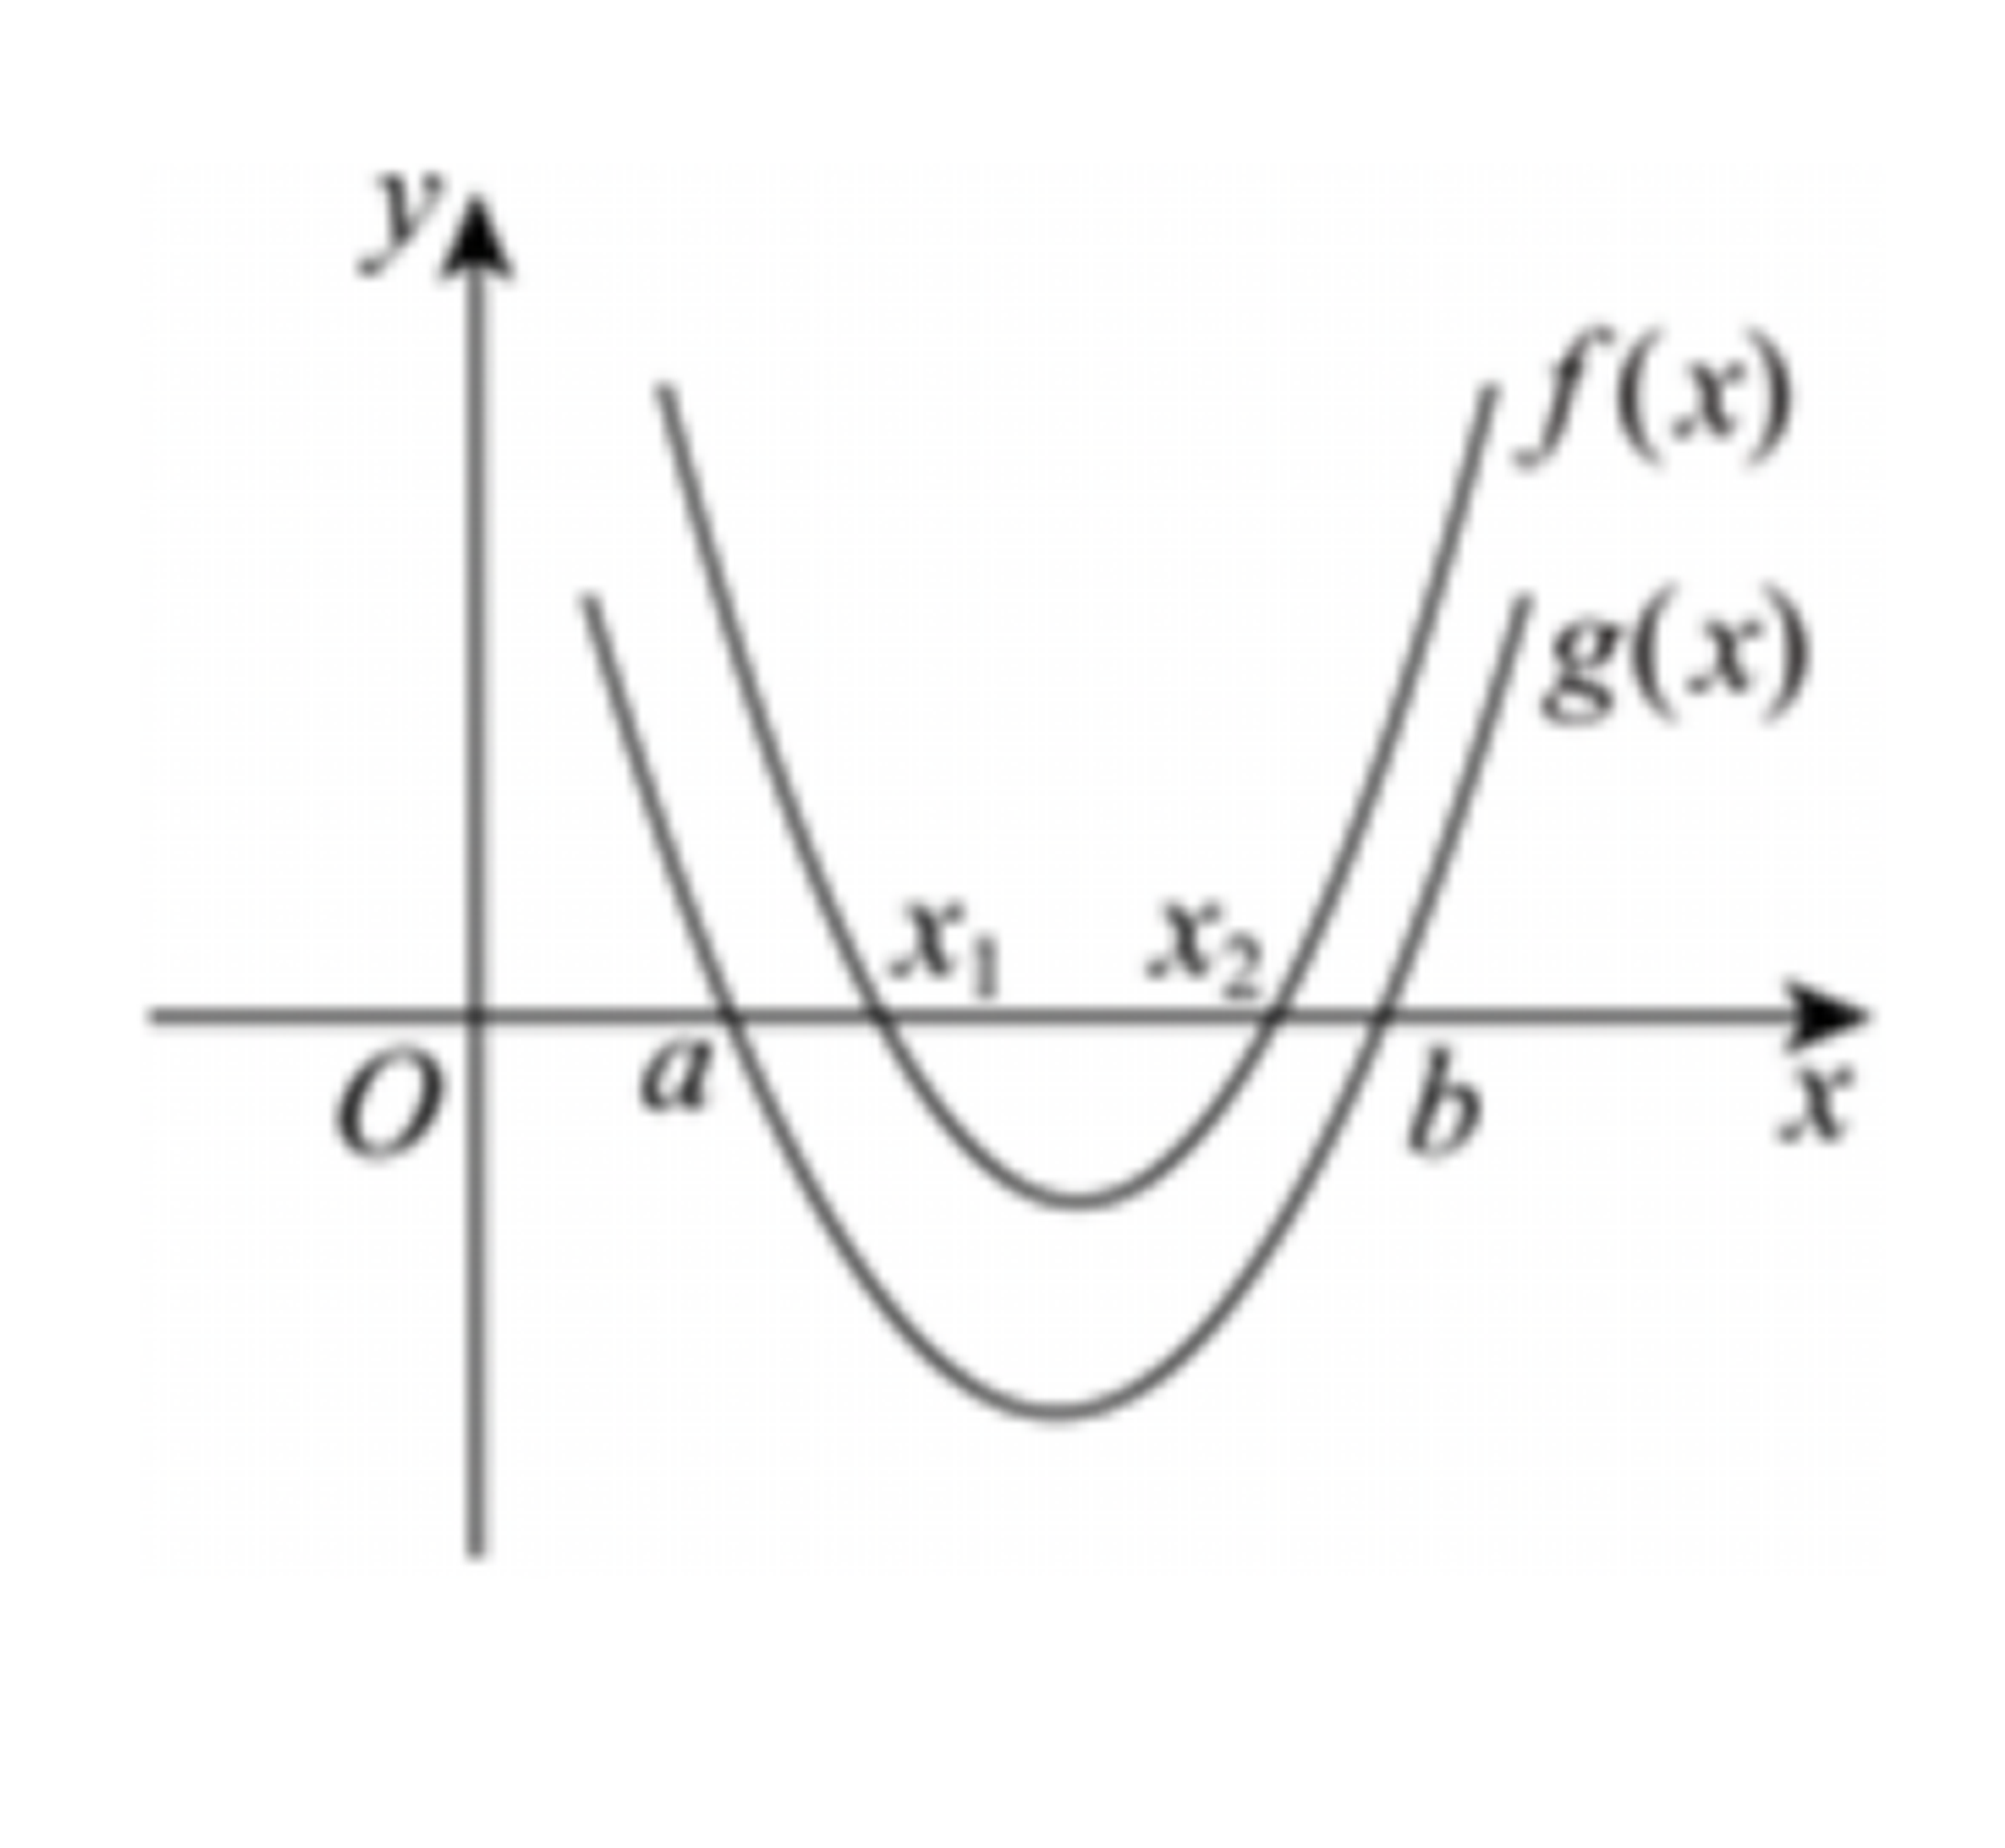
\includegraphics[width=0.30\textwidth]{figures/parabola_f_g_x1x2_h65.png}
\end{center}
\step{由图像得 $a<x_1<x_2<b$，故选 $B$.}
\solend
\fi

\end{enumerate}

\bigsec{三、解答题}

\begin{enumerate}
\setcounter{enumi}{16}

\item 已知 $a>0$，$b>0$，若 $a+b>4$，求证：$\dfrac a{b+2}$ 和 $\dfrac b{a+2}$ 中至少有一个大于 $\dfrac12$.

\ifanswer
\solbegin
\step{假设 $\dfrac a{b+2}\leqslant\dfrac12$，$\dfrac b{a+2}\leqslant\dfrac12$，}
\step{$a>0$，$b>0$，则 $a+2>0$，$b+2>0$，故 $2a\leqslant b+2$，$2b\leqslant a+2$，}
\step{两式相加得 $a+b\leqslant4$，与 $a+b>4$ 矛盾，故 $\dfrac a{b+2}$ 和 $\dfrac b{a+2}$ 中至少有一个大于 $\dfrac12$.}
\solend
\fi

\ansspace[6]

\item 已知集合 $A=\{x\mid-4<x<5\}$，$B=\{x\mid x\leqslant a-6\text{ 或 }x\geqslant a+2\}$.

\begin{enumerate}[label=(\arabic*)]

\item 若 $A\cup B=\R$，求实数 $a$ 的取值范围；

\item 若“$x\in A$”是“$x\in B$”的充分不必要条件，求实数 $a$ 的取值范围.

\end{enumerate}

\ifanswer
\solbegin
\stepm{(1)}{集合 $A=\{x\mid-4<x<5\}$，$B=\{x\mid x\leqslant a-6\text{ 或 }x\geqslant a+2\}$.}
\step{由 $A\cup B=\R$ 得 $\begin{cases}a-6\geqslant-4\\ a+2\leqslant5\end{cases}$，解得 $2\leqslant a\leqslant3$，$a$ 的取值范围为 $[2,3]$；}
\stepm{(2)}{若“$x\in A$”是“$x\in B$”的充分不必要条件，则 $A\subset B$，}
\step{则 $5\leqslant a-6$ 或 $-4\geqslant a+2$，解得 $a\leqslant-6$ 或 $a\geqslant11$.}
\solend
\fi

\ansspace[8]

% 注：原卷题干把命题 $P$ 印作“$\exists3\notin A$”（多一个存在量词），而【解析】两处均作
%     “$3\notin A$”；照录未改，见文件头“原卷笔误/存疑”③。
\item 已知集合 $A=\left\{x\mid\dfrac{x-1}{x-m}<0\right\}$，集合 $B=\left\{x\mid\left|\dfrac{x-1}{x-3}\right|\geqslant1\right\}$，命题 $P$：“$\exists3\notin A$”，命题
$Q$：$A\cap B\neq\varnothing$.

\begin{enumerate}[label=(\arabic*)]

\item 若命题 $P$ 为真命题，求 $m$ 的取值范围；

\item 若命题 $P$ 和命题 $Q$ 至少有一个为假命题，求实数 $m$ 的取值范围.

\end{enumerate}

\ifanswer
\solbegin
\stepm{(1)}{$A=\left\{x\mid\dfrac{x-1}{x-m}<0\right\}=\{x\mid(x-1)(x-m)<0\}$，}
\step{若命题 $P$：“$3\notin A$”为真命题，则 $(3-1)(3-m)\geqslant0$，解得 $m\leqslant3$，}
\step{故实数 $m$ 的取值范围为 $(-\infty,3]$；}
\stepm{(2)}{$B=\left\{x\mid\left|\dfrac{x-1}{x-3}\right|\geqslant1\right\}$，由 $\left|\dfrac{x-1}{x-3}\right|\geqslant1$，得 $\begin{cases}|x-1|\geqslant|x-3|\\ x\neq3\end{cases}$，}
\step{等价于 $\begin{cases}(x-1)^2\geqslant(x-3)^2\\ x\neq3\end{cases}$，解得 $x\geqslant2$ 且 $x\neq3$，所以 $B=[2,3)\cup(3,+\infty)$，}
\step{因为 $A=\{x\mid(x-1)(x-m)<0\}$，}
\step{当 $m=1$ 时，$A=\varnothing$，不满足 $A\cap B\neq\varnothing$，}
\step{当 $m<1$ 时，$A=(m,1)$，不满足 $A\cap B\neq\varnothing$，}
\step{当 $m>1$ 时，$A=(1,m)$，要使 $A\cap B\neq\varnothing$，则 $m>2$，}
\step{则若命题 $Q$：“$A\cap B\neq\varnothing$”为真命题时，实数 $m$ 的取值范围为 $(2,+\infty)$，}
\step{当命题 $P$ 与命题 $Q$ 都是真命题时，则 $\begin{cases}m\leqslant3\\ m>2\end{cases}$，解得 $2<m\leqslant3$，}
\step{则命题 $P$ 和命题 $Q$ 至少有一个为假命题时，得 $m\leqslant2$ 或 $m>3$，}
\step{故实数 $m$ 的取值范围为 $(-\infty,2]\cup(3,+\infty)$.}
\solend
\fi

\ansspace[8]

\item 已知函数 $y=ax^2-(a+2)x+2$，$a\in\R$.

\begin{enumerate}[label=(\arabic*)]

\item $y<3-2x$ 恒成立，求实数 $a$ 的取值范围；

% 注：原卷末句作“求实数 $a$ 的取值”（疑脱“范围”二字），照录未改，
%     见文件头“原卷笔误/存疑”⑤。
\item 若存在 $m>0$ 使关于 $x$ 的方程 $ax^2-(a+2)|x|+2=m+\dfrac1m+1$ 有四个不同的实根，
求实数 $a$ 的取值.

\end{enumerate}

\ifanswer
\solbegin
\stepm{(1)}{由题意得 $ax^2-(a+2)x+2<3-2x$ 恒成立，}
\step{即 $ax^2-ax-1<0$ 恒成立，}
\step{当 $a=0$ 时，$-1<0$ 恒成立，符合题意，}
\step{当 $a\neq0$ 时，则 $\begin{cases}a<0\\ \triangle=a^2+4a<0\end{cases}$，得 $\begin{cases}a<0\\ -4<a<0\end{cases}$，得 $-4<a<0$，}
\step{综上，$a$ 的取值范围为 $(-4,0]$.}
\stepm{(2)}{当 $m>0$ 时，令 $t=m+\dfrac1m+1\geqslant2\sqrt{m\times\dfrac1m}+1=3$，}
\step{当且仅当 $m=1$ 时取等号，}
% 注：题干只给“函数 $y=ax^2-(a+2)x+2$”，全卷未设 $f$，此处 $f(|x|)$ 无定义；
%     照录未改，见文件头“原卷笔误/存疑”④。
\step{则关于 $x$ 的方程 $f(|x|)=t$ 可化为 $a|x|^2-(a+2)|x|+2-t=0$，}
\step{关于 $x$ 的方程为 $a|x|^2-(a+2)|x|+2-t=0$ 有四个不等的实数根，}
\step{即 $ax^2-(a+2)x+2-t=0$，有两个不同的实数正根，}
\step{则 $\begin{cases}\triangle=(a+2)^2-4a(2-t)>0\\ \dfrac{a+2}a>0\\ \dfrac{2-t}a>0\end{cases}$，解得 $a<-2$，}
\step{由（1）得存在 $t\in[3,+\infty)$ 使得不等式 $4at+(a+2)^2-8a>0$ 成立，}
\step{故 $4a\times3+(a+2)^2-8a>0$，即 $a^2+8a+4>0$，}
\step{解得 $a<-4-2\sqrt3$ 或 $a>-4+2\sqrt3$，}
\step{综上，$a<-4-2\sqrt3$，所以 $a$ 的取值范围为 $(-\infty,-4-2\sqrt3)$.}
\solend
\fi

\ansspace[8]

\item 若集合 $A=B_1\cup B_2\cup\cdots\cup B_n$，其中 $B_1$、$B_2$、$\cdots$、$B_n$ 为非空集合，
$B_i\cap B_j=\varnothing$($1\leqslant i<j\leqslant n$)，则称集合 $\{B_1,B_2,\cdots,B_n\}$ 为集合 $A$ 的一个 $n$ 划分.

\begin{enumerate}[label=(\arabic*)]

\item 写出集合 $A=\{1,2,3\}$ 的所有不同的 2 划分；

\item 设 $\{B_1,B_2\}$ 为有理数集 $\Q$ 的一个 2 划分，且满足对任意 $x\in B_1$，任意 $y\in B_2$，都有
$x<y$，判断命题“$B_1$ 中的元素存在最大值，$B_2$ 中的元素存在最小值.”的真假，并说明
理由.

\item 设集合 $A=\{1,2,3,\cdots,16\}$，对于集合 $A$ 的任意一个 3 划分 $\{B_1,B_2,B_3\}$，判断是否存
在 $i\in\{1,2,3\}$，存在 $a$、$b\in B_i$，使得 $b-a\in B_i$ 成立，并说明理由.

\end{enumerate}

\ifanswer
\solbegin
% 注：原卷三个“2 划分”本有外层花括号（$\{\{1,2\},\{3\}\}$ 等），首轮误脱；
%     第二轮复核照原卷补回（原卷原样 / 本稿原错处：原脱外层花括号）。
\stepm{(1)}{集合 $A=\{1,2,3\}$ 的所有不同的 2 划分为 $\{\{1,2\},\{3\}\}$、$\{\{1,3\},\{2\}\}$、}
\step{$\{\{2,3\},\{1\}\}$.}
\stepm{(2)}{该命题为假命题，理由如下：}
\step{假设命题为真，则不妨设 $B_1$ 中元素的最大值为 $s$，$B_2$ 中元素的最小值为 $t$，}
\step{由题意得 $s<t$，所以 $s<\dfrac{s+t}2<t$，}
\step{因为 $s$ 为 $B_1$ 中元素的最大值，所以 $\dfrac{s+t}2\notin B_1$，}
\step{因为 $t$ 为 $B_2$ 中元素的最小值，所以 $\dfrac{s+t}2\notin B_2$，}
\step{因为 $B_1\cup B_2=\Q$，所以 $\dfrac{s+t}2\notin\Q$，}
\step{这与 $\dfrac{s+t}2\in\Q$ 矛盾，所以假设不成立，即命题不可能成立；}
\stepm{(3)}{由于集合 $A$ 中有 16 个元素，}
\step{所以 $B_1$、$B_2$、$B_3$ 中至少有一个集合至少包含 6 个元素，}
\step{不妨设 $B_1$ 中至少包含 6 个元素，}
\step{设 $b_1$、$b_2$、$b_3$、$b_4$、$b_5$、$b_6\in B_1$，且 $b_1<b_2<b_3<b_4<b_5<b_6$，}
\step{假设对任意 $i\in\{1,2,3\}$，对任意 $a$、$b\in B_i$，都有 $b-a\notin B_i$，}
\step{那么 $b_6-b_1$、$b_6-b_2$、$b_6-b_3$、$b_6-b_4$、$b_6-b_5\notin B_1$，}
\step{又因为 $b_6-b_1$、$b_6-b_2$、$b_6-b_3$、$b_6-b_4$、$b_6-b_5\in A$，}
\step{所以 $b_6-b_1$、$b_6-b_2$、$b_6-b_3$、$b_6-b_4$、$b_6-b_5\in B_2\cup B_3$，}
\step{则 $B_2$、$B_3$ 中必有一个集合}
\step{至少包含 $b_6-b_1$、$b_6-b_2$、$b_6-b_3$、$b_6-b_4$、$b_6-b_5$ 中的 3 个元素，}
\step{不妨设这 3 个元素为 $a_1$、$a_2$、$a_3\in B_2$，$a_1<a_2<a_3$，}
\step{由假设得 $a_3-a_1$、$a_3-a_2$、$a_2-a_1\notin B_2$，}
\step{对任意 $i$、$j$($1\leqslant j<i\leqslant3$)，存在 $m$、$n$($1\leqslant m<n\leqslant5$)，}
\step{都有 $a_i-a_j=b_6-b_m-b_6+b_n=b_n-b_m\notin B_1$，}
\step{又因为 $a_3-a_1$、$a_3-a_2$、$a_2-a_1\in B_3$，而 $a_3-a_1-(a_3-a_2)=a_2-a_1$，}
\step{与假设矛盾，所以假设不成立，}
\step{即存在 $i\in\{1,2,3\}$，存在 $a$、$b\in B_i$，使得 $b-a\in B_i$.}
\solend
\fi

\ansspace*[10]

\end{enumerate}

\end{document}
"
%
% 原始材料：微信公众号“魔都数学加油站”文章，作者破晓，连载“27学年高一65”；
% 原文标题“27学年高一65——2026-2027年上海市大同中学高一上10月月考”；
% 原文链接：https://mp.weixin.qq.com/s/h9ctuk-ByE1Vfg2Rx2C6bw。
% 页面标注发布时间 2026-10-17 21:58（上海）。
% 本次转录只据 `原图/高一65_大同中学_10月月考/` 的 11 张 PNG 逐页读图。
% 正文为 11 张 PNG 页（`01..11.png`）：
% 第 06、11 页 2560×3620，第 01、02、03、04、05、07、08、09、10 页 4762×6735
% （**同一篇各页分辨率不同**），均按页序读取。11 页全为试卷正文页（卷首标题在第 1 页页顶，
% 卷末解答题第 21 题解析止于第 11 页），无封面页、目录页、二维码或宣传页。
% 粉色斜排“魔都数学加油站”为卷面水印，与公众号页脚一并未录入。
%
% 卷首标题：照卷面印作“2026--2027 年大同中学高一上 10 月月考”，年份区间按全稿惯例排 en dash。
% 原卷只有一行标题、无副标题。
%
% 篇幅与题号：原卷自第 3 题起编号（第 1、2 题不在本卷内）。填空题 3—12（10 题）、
% 选择题 13—16（4 题）、解答题 17—21（5 题），共 19 题。本稿沿用原节与原题号，
% 只改排为全稿统一的大节样式（原卷小节标题为“一、填空题”“二、选择题”“三、解答题”）。
%
% 讲评版：原卷每题下直接印【答案】或【解析】。**只印【答案】的 4 题**（第 3、4、7、10 题），
% 本稿只给 \ans{}；其余 15 题都印【解析】（按全稿口径这类题不另提 \ans{}——第 12、13、14、
% 15、16 题的结论写在解析末句（“故选 B”“综上，n 的最大值为 14”等），亦照录在解析内）。
% 全卷无“答案印在题干括号内”的题（第 13—16 题的选择题括号内均空白）。
%
% 副标题：原卷未印副标题。本稿按“知识模块”口径标作“集合与常用逻辑用语、不等式”：
% 19 题中集合与常用逻辑用语 10 题（第 3、4、6、8、12、14、15、18、19、21 题），
% 不等式 9 题（含等式恒等、不等式性质、二次不等式、恒成立、基本不等式、不等式的证明：
% 第 5、7、9、10、11、13、16、17、20 题），两类均超过三分之一，故并标。口径同 高一63。
%
% 与原卷的排版差异：
%   ① 原卷每题下直接印【答案】/【解析】，本稿按全稿惯例将答案与解析置于答案版，试卷版保持干净；
%   ② 原卷未印副标题，本稿按“知识模块”口径补出；
%   ③ 原卷填空横线约四个字宽，本稿按全稿惯例统一排 \blankline[4.4em]；
%   ④ 原卷数集记号全为斜体：实数集作 $R$（第 6 题两处、第 8 题两处、第 15 题解析、第 18 题、
%      第 20 题题干），自然数集作 $N$（第 12 题题干“$n\in N,n\geqslant1$”），有理数集作 $Q$
%      （第 21 题 (2) 题干与解析共 4 处），本稿按全稿惯例统一改用 $\R$、$\N$、$\Q$
%      （同 高一63 排版差异④：记号归一）；空集记号原卷作 $\varnothing$，照录；
%   ⑤ 原卷用描述法时竖线排细竖“$|$”（如 $\{x|0<x<3\}$、$\{x|(x-1)(x-m)<0\}$），
%      本稿按全稿惯例排 \mid；
%   ⑥ 原卷判别式印作“$\triangle$”（第 8、14 题解析各 1 处、第 20 题解析 2 处，共 4 处），
%      本稿照录用 \triangle（同 高一39 成例），未改作 \Delta；
%   ⑦ 第 18—21 题的子问原卷各自另起一行、以“（1）”“（2）”标号，本稿按全稿惯例用
%      enumerate 的 (1)(2)(3)；解析中的子问标号一律用 \stepm{(1)}{…}；
%      第 18—21 题解析（原文以“（1）”“（2）”“（3）”冠于解析首句）同此；
%   ⑧ 选择题的作答括号原卷排半角“(　　)”（第 13—16 题括号内均空白），
%      本稿按全稿惯例排 \mbox{（\quad）}；选项字母后的句点照原卷排“A.”“B.”；
%   ⑨ 每道解答题原卷未留作答空白，本稿按全稿惯例加 \ansspace（末题用 \ansspace*）；
%   ⑩ 原卷在数学式内多处用半角逗号（如 $\{x|0<x<3\},B=\{x|x>2\}$、$m\in I_{14},k\in I_{14}$），
%      均照录未强改；句末句点按全稿惯例排西文句点。
%
% 原卷笔误/存疑（均照录未改，正文对应处另有 % 注）：
%   ① 第 13 题题干“下列不等式中一定成立是（　　）”脱一个“的”（当作“一定成立的是”），
%      8 倍放大确认非水印遮挡，本稿照录；
%   ② 第 15 题【解析】末段把题干条件“$x\geqslant10$”写成“$x\geqslant1$”
%      （“所以 $x+2+\frac{16}{x+2}(x\geqslant1)$ 的最小值不为 8”），与同段前面“令 $t=x+2$，
%      则 $t\geqslant12$”不合，本稿照录；
%   ③ 第 19 题题干把命题 $P$ 印作“$\exists3\notin A$”（多一个存在量词），而【解析】两处
%      均作“$3\notin A$”，前后记号不一，本稿照录；
%   ④ 第 20 题【解析】(2) 出现 $f(|x|)$，但题干只给“函数 $y=ax^2-(a+2)x+2$”、全卷未设 $f$，
%      本稿照录；
%   ⑤ 第 20 题 (2) 题干末句作“求实数 $a$ 的取值”（疑脱“范围”二字），本稿照录；
%   ⑥ 第 12 题【解析】第 18 步“它与 $P_n$ 中的任何其他数之和都不是整数”，该段所论为 $P_{14}$
%      （前后均作 $P_{14}$），此处 $P_n$ 疑当作 $P_{14}$，本稿照录。
%
% 第二轮复核（2026-10-18）订正「本稿抄错原卷」一处：
%   第 21 题 (1)【解析】原卷本作“$\{\{1,2\},\{3\}\}$、$\{\{1,3\},\{2\}\}$、$\{\{2,3\},\{1\}\}$”，
%   有外层花括号；首轮误脱外层花括号，并曾在文件头误记为“原卷未加外层花括号”（原第 ⑦ 条，
%   已撤销）。本次照原卷补回，正文对应处另有 % 注。
%
% 插图：第 16 题【解析】内有 1 幅图（两条开口向上的抛物线 $f(x)$、$g(x)$ 与 $x$ 轴交点
% 标 $a$、$x_1$、$x_2$、$b$，纵轴标 $y$、原点 $O$），解析第三行“画出函数 $g(x)$ 与函数 $f(x)$
% 的图像，如图所示”即指此图；取原卷截图（06.png，2560×3620）右半幅，4× LANCZOS 放大，
% 存 figures/parabola_f_g_x1x2_h65.png。该图在【解析】内，仅答案版出。
%
\documentclass[a4paper,11pt]{article}
\usepackage{common}

\begin{document}

\examtitlest[3]{2026--2027 年大同中学高一上 10 月月考}{集合与常用逻辑用语、不等式}

\bigsec{一、填空题}

\begin{enumerate}
\setcounter{enumi}{2}

\item 已知集合 $A=\{x\mid0<x<3\}$,$B=\{x\mid x>2\}$，则集合 $A\cup B=$\blankline[4.4em].

\ifanswer
\ans{$(0,+\infty)$}
\fi

\item “$x>1$ 或 $y>1$”的否定形式是\blankline[4.4em].

\ifanswer
\ans{$x\leqslant1$ 且 $y\leqslant1$}
\fi

\item 已知等式 $2x^2+3x+4=a(2x+1)(x+1)+b$ 恒成立，则常数 $a-b=$\blankline[4.4em].

\ifanswer
\solbegin
\step{因为等式 $2x^2+3x+4=a(2x+1)(x+1)+b$ 恒成立，}
\step{所以 $a(2x+1)(x+1)+b=2ax^2+3ax+a+b=2x^2+3x+4$，}
\step{所以 $\begin{cases}2a=2\\ 3a=3\\ a+b=4\end{cases}$，解得 $\begin{cases}a=1\\ b=3\end{cases}$，所以 $a-b=-2$.}
\solend
\fi

\item 全集为 $U=\R$，$A=\{x\mid|x|\geqslant2\}$，$B=\{y\mid y=x^2+1,x\in\R\}$，则 $A\cup\bar B=$\blankline[4.4em].

\ifanswer
\solbegin
\step{由题意得集合 $A=\{x\mid x\geqslant2\text{ 或 }x\leqslant-2\}$，}
\step{因为 $x^2+1\geqslant1$，所以集合 $B=\{x\mid x\geqslant1\}$，所以 $\bar B=\{x\mid x<1\}$，}
\step{则 $A\cup\bar B=\{x\mid x\geqslant2\text{ 或 }x<1\}$.}
\solend
\fi

\item 已知 $|x+3|+|x-5|=8$，则实数 $x$ 的取值范围为\blankline[4.4em].

\ifanswer
\ans{$[-3,5]$}
\fi

\item 已知集合 $A=\{x\in\R\mid ax^2+2x+1=0,a\in\R\}$ 只有一个元素，则 $a$ 的值为\blankline[4.4em].

\ifanswer
\solbegin
\step{当 $a=0$ 时，$A=\left\{-\dfrac12\right\}$；}
\step{当 $a\neq0$ 时，若集合 $A$ 只有一个元素，由 $\triangle=4-4a=0$ 得 $a=1$.}
\step{综上，当 $a=0$ 或 $a=1$ 时，集合 $A$ 只有一个元素.}
\solend
\fi

\item 已知不等式 $-x^2+bx+c>0$ 的解集为 $(3,4)$，则不等式 $cx^2+bx-1<0$ 的解集为\blankline[4.4em].

\ifanswer
\solbegin
\step{由题意得 3，4 是方程 $-x^2+bx+c=0$ 的两个实数根，}
\step{所以 $\begin{cases}3+4=b\\ 3\times4=-c\end{cases}$，得 $b=7$，$c=-12$，}
\step{则不等式 $cx^2+bx-1<0$，即为 $-12x^2+7x-1<0$，即 $12x^2-7x+1>0$，}
\step{化简得 $(3x-1)(4x-1)>0$，解得 $x<\dfrac14$ 或 $x>\dfrac13$，}
\step{即不等式 $cx^2+bx-1<0$ 的解集为 $\left(-\infty,\dfrac14\right)\cup\left(\dfrac13,+\infty\right)$.}
\solend
\fi

\item 对于区间 $(m,n)$，我们将 $n-m$ 的值称为该区间的长度. 若关于 $x$ 的不等式
$x^2+ax+a<0$ 有解，且解集的区间长度不超过 $2\sqrt3$，则实数 $a$ 的取值范围是\blankline[4.4em].

\ifanswer
\ans{$[-2,0)\cup(4,6]$}
\fi

\item 当 $x>0$ 时，关于 $x$ 的不等式 $(ax-1)(x^2+bx-4)\geqslant0$ 恒成立，则 $b+\dfrac2a$ 的最小值
为\blankline[4.4em].

\ifanswer
\solbegin
\step{由题意 $a\neq0$；}
\step{若 $a<0$，则 $x>0$ 时 $ax-1<0$ 恒成立，需 $x^2+bx-4\leqslant0$ 对一切 $x>0$ 成立，}
\step{而 $y=x^2+bx-4$ 的图象开口向上，当 $x$ 充分大时必为正值，矛盾，故 $a>0$.}
\step{当 $a>0$ 时，$ax-1=a\left(x-\dfrac1a\right)$，故原条件化为 $\left(x-\dfrac1a\right)(x^2+bx-4)\geqslant0$：}
\step{若 $0<x<\dfrac1a$，则 $x-\dfrac1a<0$，需 $x^2+bx-4\leqslant0$；}
\step{若 $x>\dfrac1a$，则 $x-\dfrac1a>0$，需 $x^2+bx-4\geqslant0$；}
\step{由 $y=x^2+bx-4$ 的连续性知 $x=\dfrac1a$ 是它的零点，}
\step{即 $\dfrac1{a^2}+\dfrac ba-4=0$，得 $b=4a-\dfrac1a$；}
\step{此时 $x^2+bx-4=x^2+\left(4a-\dfrac1a\right)x-4=(x+4a)\left(x-\dfrac1a\right)$，}
\step{由 $a>0$、$x>0$ 得 $x+4a>0$，}
\step{其符号与 $x-\dfrac1a$ 一致，故能与 $ax-1$ 同号，原不等式确在 $x>0$ 上恒成立.}
\step{于是 $b+\dfrac2a=4a-\dfrac1a+\dfrac2a=4a+\dfrac1a\geqslant2\sqrt{4a\cdot\dfrac1a}=4$，}
\step{当且仅当 $a=\dfrac12$ 时取等号，故最小值为 4.}
\solend
\fi

\item 设集合 $I_n=\{1,2,\cdots,n\}$，$n\in\N$，$n\geqslant1$，集合 $P_n=\left\{\dfrac m{\sqrt k}\mid m\in I_n,k\in I_n\right\}$，若 $P_n$ 的子集 $A$
中任意两个元素之和不是整数的平方，则称 $A$ 为“人文集”. 那么使 $P_n$ 能分成两个交集为空
集的“人文集”的并集，且这两个人文集的并集恰为 $P_n$ 时，$n$ 的最大值是\blankline[4.4em].

\ifanswer
\solbegin
\step{先证当 $n\geqslant15$ 时，$P_n$ 不能分成两个不相交的人文集的并集.}
\step{假设当 $n\geqslant15$ 时，$P_n$ 可以分成两个不相交的人文集的并集，}
\step{设 $A$ 和 $B$ 为两个不相交的人文集，使 $A\cup B=P_n\supseteq I_n$.}
\step{不妨设 $1\in A$，则由于 $1+3=2^2$，所以 $3\notin A$，即 $3\in B$.}
\step{同理可得，$6\in A$，$10\in B$. 又推出 $15\in A$，}
\step{但 $1+15=4^2$，这与 $A$ 为人文集相矛盾.}
\step{再证 $P_{14}$ 满足要求. 当 $k=1$ 时，$P_{14}=\left\{\dfrac m{\sqrt k}\mid m\in I_{14},k\in I_{14}\right\}$，}
\step{可以分成 2 个人文集的并集.}
\step{事实上，只要取 $A_1=\{1,2,4,6,9,11,13\}$，$B_1=\{3,5,7,8,10,12,14\}$，}
\step{则 $A_1$ 和 $B_1$ 都是人文集，且 $A_1\cup B_1=P_{14}$.}
\step{当 $k=4$ 时，集合 $\left\{\dfrac m{\sqrt k}\mid m\in I_{14}\right\}$ 中，除整数外，}
\step{剩下的数组成集合 $\left\{\dfrac12,\dfrac32,\dfrac52,\cdots,\dfrac{13}2\right\}$，}
\step{可以分为下列 2 个人文集的并：$A_2=\left\{\dfrac12,\dfrac52,\dfrac92,\dfrac{11}2\right\}$，$B_2=\left\{\dfrac32,\dfrac72,\dfrac{13}2\right\}$.}
\step{当 $k=9$ 时，集合 $\left\{\dfrac m{\sqrt k}\mid m\in I_{14}\right\}$ 中，除整数外，}
\step{剩下的数组成集合 $\left\{\dfrac13,\dfrac23,\dfrac43,\dfrac53,\cdots,\dfrac{13}3,\dfrac{14}3\right\}$，}
\step{可以分为下列 2 个人文集的并：$A_3=\left\{\dfrac13,\dfrac43,\dfrac53,\dfrac{10}3,\dfrac{13}3\right\}$，$B_3=\left\{\dfrac23,\dfrac73,\dfrac83,\dfrac{11}3,\dfrac{14}3\right\}$.}
\step{最后，集合 $C=\left\{\dfrac m{\sqrt k}\mid m\in I_{14},k\in I_{14},k\neq1,4,9\right\}$ 中的数的分母都是无理数，}
% 注：本行原卷作“$P_n$”，而该段所论为 $P_{14}$（前后均作 $P_{14}$），疑当作 $P_{14}$；
%     照录未改，见文件头“原卷笔误/存疑”⑥。
\step{它与 $P_n$ 中的任何其他数之和都不是整数，}
\step{因此，令 $A=A_1\cup A_2\cup A_3\cup C$，$B=B_1\cup B_2\cup B_3$，}
\step{则 $A$ 和 $B$ 是不相交的人文集，且 $A\cup B=P_{14}$.}
\step{综上，$n$ 的最大值为 14.}
\solend
\fi

\end{enumerate}

\bigsec{二、选择题}

\begin{enumerate}
\setcounter{enumi}{12}

% 注：原卷题干“下列不等式中一定成立是”脱一个“的”（当作“一定成立的是”），
%     照录未改，见文件头“原卷笔误/存疑”①。
\item 已知 $a>b$，下列不等式中一定成立是\mbox{（\quad）}

\keepwithprev
A. $a^2>b^2$\qquad B. $ac^2>bc^2$\qquad C. $\dfrac1a<\dfrac1b$\qquad D. $a+3>b-4$

\ifanswer
\solbegin
\step{对于 $A$，当 $a=-2$，$b=-4$ 时，不等式不成立，故 $A$ 错误；}
\step{对于 $B$，当 $c=0$ 时，不等式不成立，故 $B$ 错误；}
\step{对于 $C$，当 $a=2$，$b=-4$ 时，不等式不成立，故 $C$ 错误；}
\step{对于 $D$，因为 $a>b$，$3>-4$，必有 $a+3>b-4$ 成立，故 $D$ 正确.}
\step{故选 $D$.}
\solend
\fi

\item 已知 $a$ 为实数，那么“$|a|\leqslant2$”是“方程 $x^2+ax+1=0$ 没有实数解”的\mbox{（\quad）}

\keepwithprev
A. 充分而不必要条件\qquad B. 必要而不充分条件

C. 充要条件\qquad D. 既不充分也不必要条件

\ifanswer
\solbegin
\step{由方程 $x^2+ax+1=0$ 没有实数解，得 $\triangle=a^2-4<0$，则 $|a|<2$，}
\step{由 $|a|<2$ 得 $|a|\leqslant2$，反之不成立，}
\step{所以“$|a|\leqslant2$”是“方程 $x^2+ax+1=0$ 没有实数解”的必要而不充分条件.}
\step{故选 $B$.}
\solend
\fi

\item 下列命题为真命题的是\mbox{（\quad）}

\keepwithprev
A. $a>b>0$，当 $m>0$ 时，$\dfrac{a+m}{b+m}>\dfrac ab$

B. 集合 $A=\{x\mid y=x^2+1\}$ 与集合 $B=\{y\mid y=x^2+1\}$ 是相同的集合

C. 若 $b<a<0$，$m<0$，则 $\dfrac ma>\dfrac mb$

D. $x+2+\dfrac{16}{x+2}(x\geqslant10)$ 最小值为 8

\ifanswer
\solbegin
\step{对于 $A$，$\dfrac{a+m}{b+m}-\dfrac ab=\dfrac{b(a+m)-a(b+m)}{b(b+m)}=\dfrac{m(b-a)}{b(b+m)}$，}
\step{因为 $a>b>0$，$m>0$，所以 $b(b+m)>0$，$m(b-a)<0$，}
\step{所以 $\dfrac{a+m}{b+m}-\dfrac ab=\dfrac{m(b-a)}{b(b+m)}<0$，}
\step{即 $a>b>0$，当 $m>0$ 时，$\dfrac{a+m}{b+m}<\dfrac ab$，故 $A$ 错误；}
\step{对于 $B$，集合 $A=\{x\mid y=x^2+1\}=\R$，集合 $B=\{y\mid y=x^2+1\}=\{y\mid y\geqslant1\}$，}
\step{所以 $A\neq B$，故 $B$ 错误；}
\step{对于 $C$，$\dfrac ma-\dfrac mb=\dfrac{m(b-a)}{ab}$，}
\step{因为 $b<a<0$，$m<0$，所以 $ab>0$，$m(b-a)>0$，}
\step{所以 $\dfrac ma-\dfrac mb=\dfrac{m(b-a)}{ab}>0$，即 $\dfrac ma>\dfrac mb$，故 $C$ 正确；}
\step{对于 $D$，令 $t=x+2$，则 $t\geqslant12$，表达式变为 $t+\dfrac{16}t$，}
\step{$t+\dfrac{16}t\geqslant2\sqrt{t\cdot\dfrac{16}t}=8$，当且仅当 $t=4$ 时取等号，即等号不成立，}
% 注：原卷本行把题干条件“$x\geqslant10$”写成“$x\geqslant1$”，与同段“$t\geqslant12$”不合；
%     照录未改，见文件头“原卷笔误/存疑”②。
\step{所以 $x+2+\dfrac{16}{x+2}(x\geqslant1)$ 的最小值不为 8，故 $D$ 错误.}
\step{故选 $C$.}
\solend
\fi

\item 已知实数 $a<b$，关于 $x$ 的不等式 $x^2-(a+b)x+ab+\dfrac12<0$ 的解集为 $(x_1,x_2)$，则实数 $a$、
$b$、$x_1$、$x_2$ 从小到大的排列是\mbox{（\quad）}

\keepwithprev
A. $x_1<a<b<x_2$\qquad B. $a<x_1<x_2<b$\qquad C. $a<x_1<b<x_2$\qquad D. $x_1<a<x_2<b$

\ifanswer
\solbegin
\step{不等式 $x^2-(a+b)x+ab+\dfrac12<0$ 可化为 $(x-a)(x-b)+\dfrac12<0$，}
\step{设 $g(x)=(x-a)(x-b)$，$f(x)=g(x)+\dfrac12$，}
\step{画出函数 $g(x)$ 与函数 $f(x)$ 的图像，如图所示，}
% 图在【解析】内（仅答案版出），取原卷截图（06.png，2560×3620）右半幅，4× LANCZOS 放大。
\begin{center}
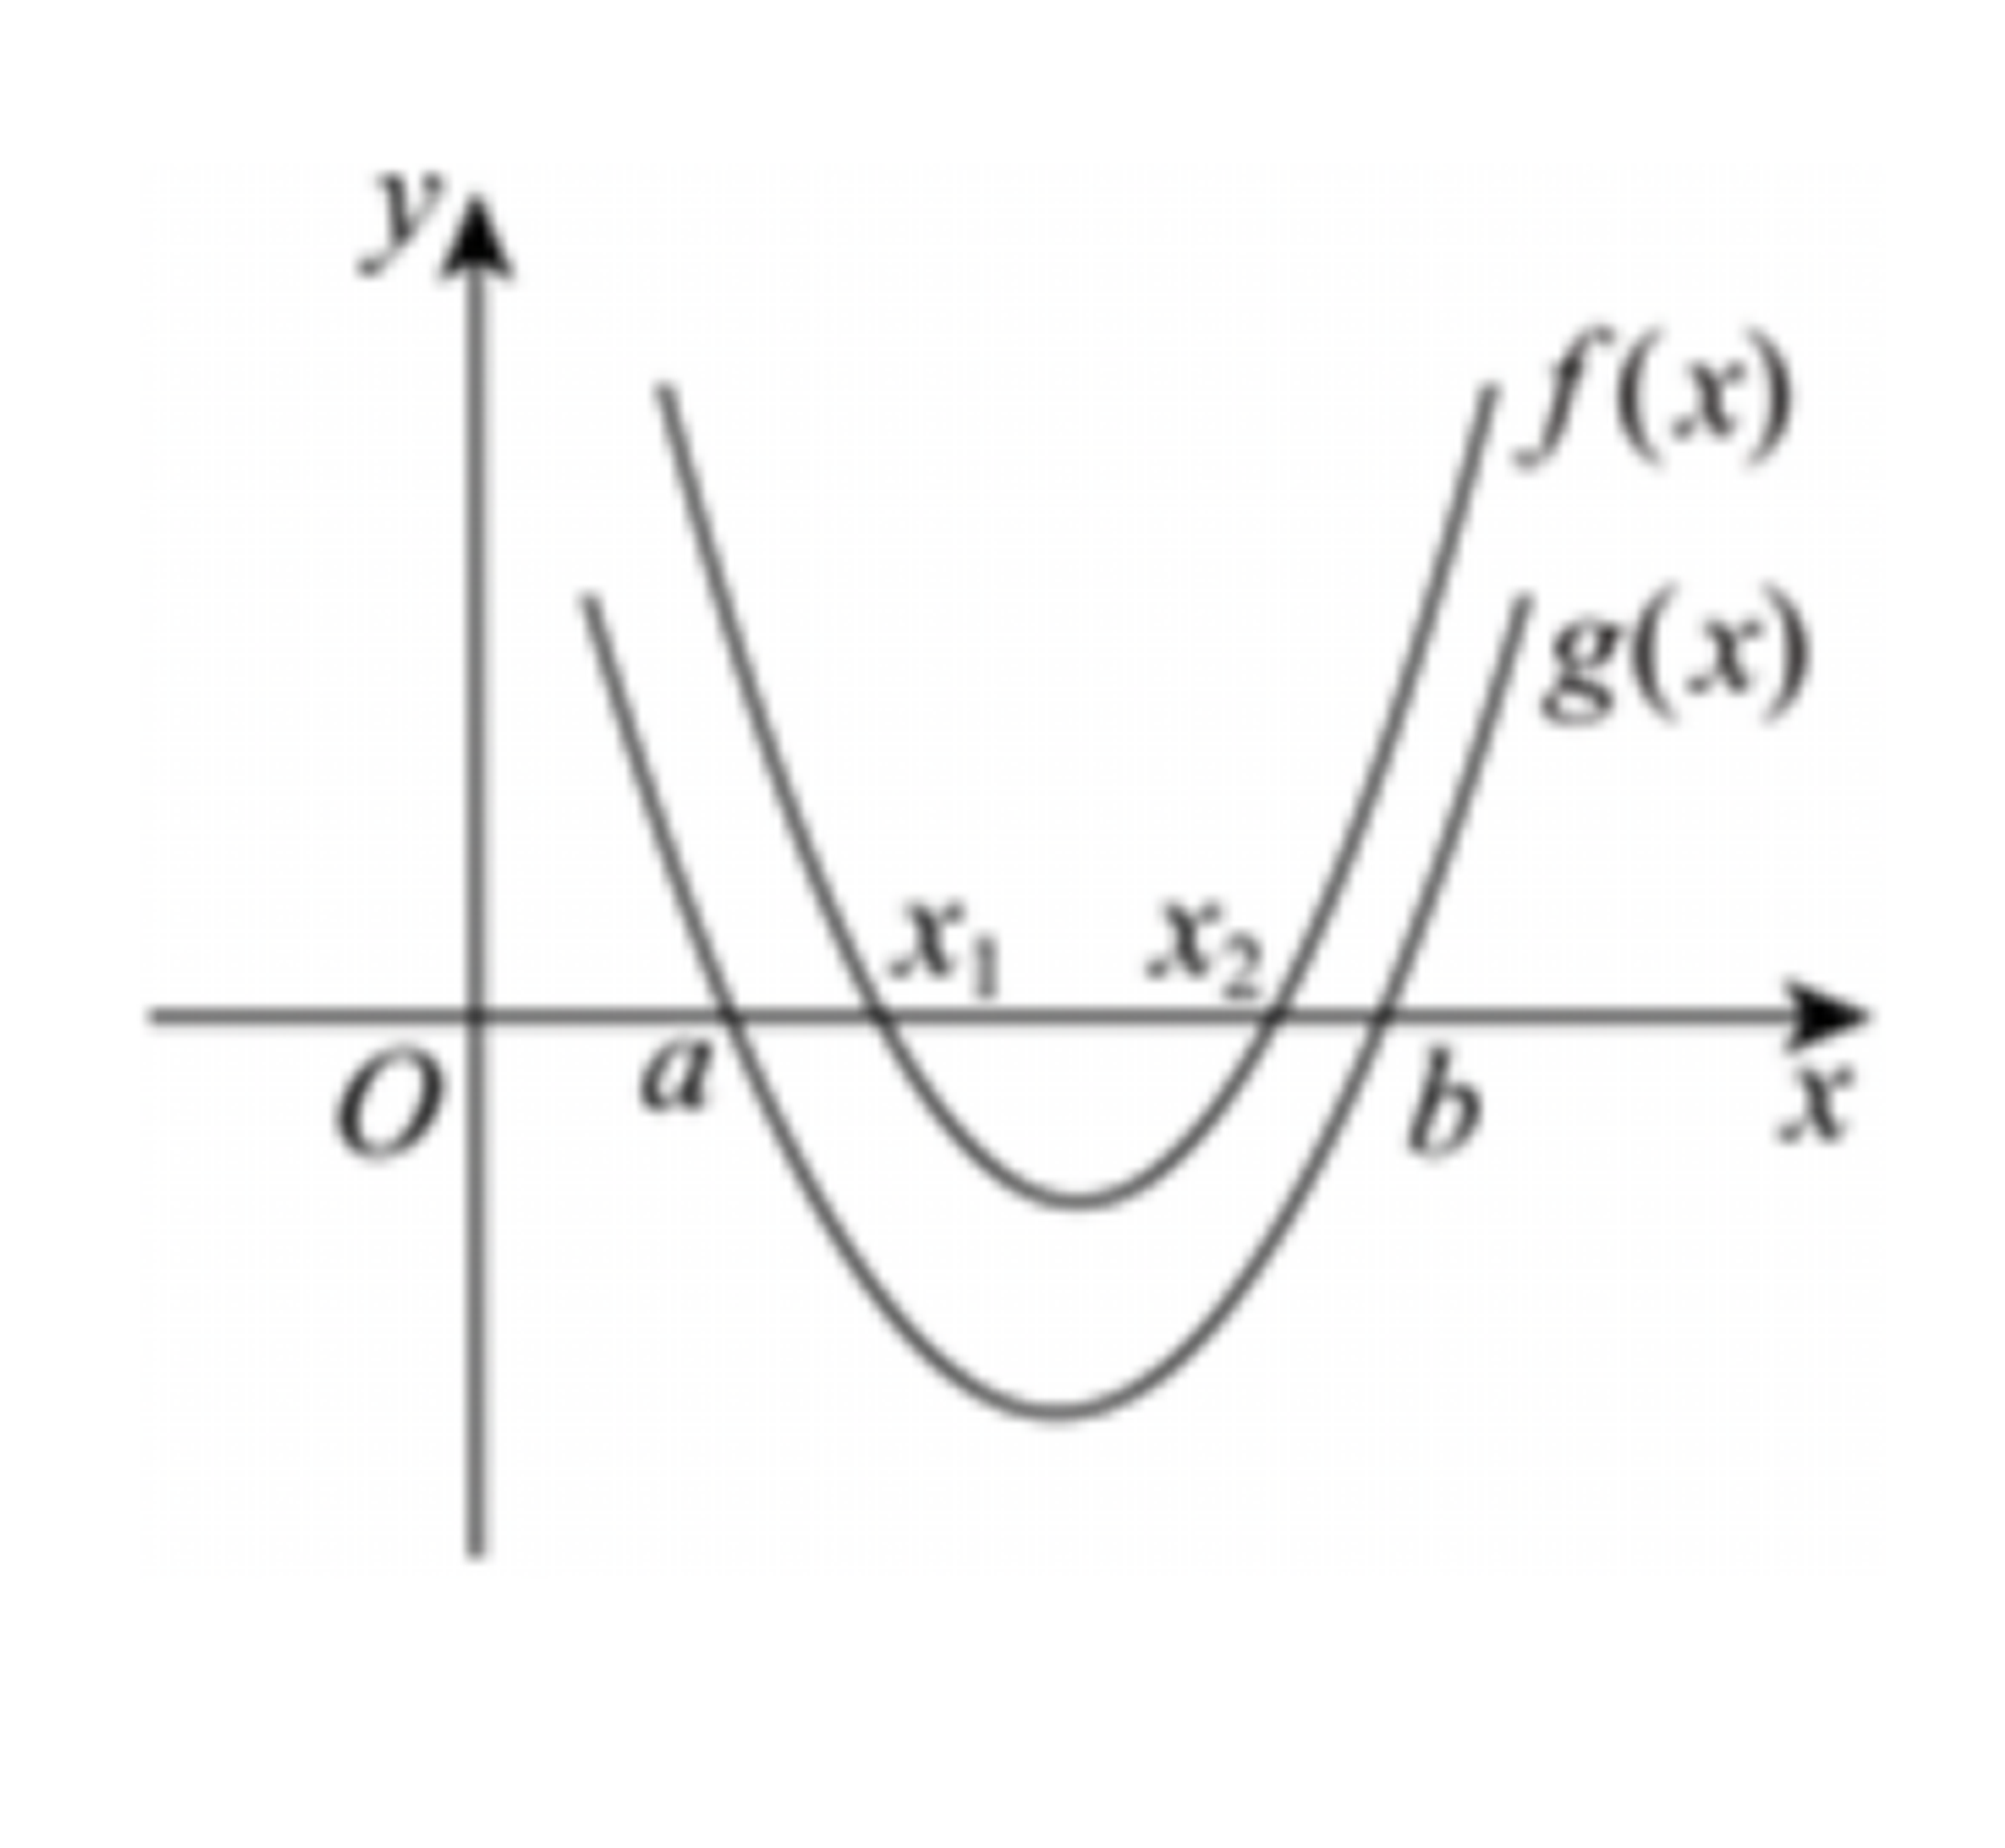
\includegraphics[width=0.30\textwidth]{figures/parabola_f_g_x1x2_h65.png}
\end{center}
\step{由图像得 $a<x_1<x_2<b$，故选 $B$.}
\solend
\fi

\end{enumerate}

\bigsec{三、解答题}

\begin{enumerate}
\setcounter{enumi}{16}

\item 已知 $a>0$，$b>0$，若 $a+b>4$，求证：$\dfrac a{b+2}$ 和 $\dfrac b{a+2}$ 中至少有一个大于 $\dfrac12$.

\ifanswer
\solbegin
\step{假设 $\dfrac a{b+2}\leqslant\dfrac12$，$\dfrac b{a+2}\leqslant\dfrac12$，}
\step{$a>0$，$b>0$，则 $a+2>0$，$b+2>0$，故 $2a\leqslant b+2$，$2b\leqslant a+2$，}
\step{两式相加得 $a+b\leqslant4$，与 $a+b>4$ 矛盾，故 $\dfrac a{b+2}$ 和 $\dfrac b{a+2}$ 中至少有一个大于 $\dfrac12$.}
\solend
\fi

\ansspace[6]

\item 已知集合 $A=\{x\mid-4<x<5\}$，$B=\{x\mid x\leqslant a-6\text{ 或 }x\geqslant a+2\}$.

\begin{enumerate}[label=(\arabic*)]

\item 若 $A\cup B=\R$，求实数 $a$ 的取值范围；

\item 若“$x\in A$”是“$x\in B$”的充分不必要条件，求实数 $a$ 的取值范围.

\end{enumerate}

\ifanswer
\solbegin
\stepm{(1)}{集合 $A=\{x\mid-4<x<5\}$，$B=\{x\mid x\leqslant a-6\text{ 或 }x\geqslant a+2\}$.}
\step{由 $A\cup B=\R$ 得 $\begin{cases}a-6\geqslant-4\\ a+2\leqslant5\end{cases}$，解得 $2\leqslant a\leqslant3$，$a$ 的取值范围为 $[2,3]$；}
\stepm{(2)}{若“$x\in A$”是“$x\in B$”的充分不必要条件，则 $A\subset B$，}
\step{则 $5\leqslant a-6$ 或 $-4\geqslant a+2$，解得 $a\leqslant-6$ 或 $a\geqslant11$.}
\solend
\fi

\ansspace[8]

% 注：原卷题干把命题 $P$ 印作“$\exists3\notin A$”（多一个存在量词），而【解析】两处均作
%     “$3\notin A$”；照录未改，见文件头“原卷笔误/存疑”③。
\item 已知集合 $A=\left\{x\mid\dfrac{x-1}{x-m}<0\right\}$，集合 $B=\left\{x\mid\left|\dfrac{x-1}{x-3}\right|\geqslant1\right\}$，命题 $P$：“$\exists3\notin A$”，命题
$Q$：$A\cap B\neq\varnothing$.

\begin{enumerate}[label=(\arabic*)]

\item 若命题 $P$ 为真命题，求 $m$ 的取值范围；

\item 若命题 $P$ 和命题 $Q$ 至少有一个为假命题，求实数 $m$ 的取值范围.

\end{enumerate}

\ifanswer
\solbegin
\stepm{(1)}{$A=\left\{x\mid\dfrac{x-1}{x-m}<0\right\}=\{x\mid(x-1)(x-m)<0\}$，}
\step{若命题 $P$：“$3\notin A$”为真命题，则 $(3-1)(3-m)\geqslant0$，解得 $m\leqslant3$，}
\step{故实数 $m$ 的取值范围为 $(-\infty,3]$；}
\stepm{(2)}{$B=\left\{x\mid\left|\dfrac{x-1}{x-3}\right|\geqslant1\right\}$，由 $\left|\dfrac{x-1}{x-3}\right|\geqslant1$，得 $\begin{cases}|x-1|\geqslant|x-3|\\ x\neq3\end{cases}$，}
\step{等价于 $\begin{cases}(x-1)^2\geqslant(x-3)^2\\ x\neq3\end{cases}$，解得 $x\geqslant2$ 且 $x\neq3$，所以 $B=[2,3)\cup(3,+\infty)$，}
\step{因为 $A=\{x\mid(x-1)(x-m)<0\}$，}
\step{当 $m=1$ 时，$A=\varnothing$，不满足 $A\cap B\neq\varnothing$，}
\step{当 $m<1$ 时，$A=(m,1)$，不满足 $A\cap B\neq\varnothing$，}
\step{当 $m>1$ 时，$A=(1,m)$，要使 $A\cap B\neq\varnothing$，则 $m>2$，}
\step{则若命题 $Q$：“$A\cap B\neq\varnothing$”为真命题时，实数 $m$ 的取值范围为 $(2,+\infty)$，}
\step{当命题 $P$ 与命题 $Q$ 都是真命题时，则 $\begin{cases}m\leqslant3\\ m>2\end{cases}$，解得 $2<m\leqslant3$，}
\step{则命题 $P$ 和命题 $Q$ 至少有一个为假命题时，得 $m\leqslant2$ 或 $m>3$，}
\step{故实数 $m$ 的取值范围为 $(-\infty,2]\cup(3,+\infty)$.}
\solend
\fi

\ansspace[8]

\item 已知函数 $y=ax^2-(a+2)x+2$，$a\in\R$.

\begin{enumerate}[label=(\arabic*)]

\item $y<3-2x$ 恒成立，求实数 $a$ 的取值范围；

% 注：原卷末句作“求实数 $a$ 的取值”（疑脱“范围”二字），照录未改，
%     见文件头“原卷笔误/存疑”⑤。
\item 若存在 $m>0$ 使关于 $x$ 的方程 $ax^2-(a+2)|x|+2=m+\dfrac1m+1$ 有四个不同的实根，
求实数 $a$ 的取值.

\end{enumerate}

\ifanswer
\solbegin
\stepm{(1)}{由题意得 $ax^2-(a+2)x+2<3-2x$ 恒成立，}
\step{即 $ax^2-ax-1<0$ 恒成立，}
\step{当 $a=0$ 时，$-1<0$ 恒成立，符合题意，}
\step{当 $a\neq0$ 时，则 $\begin{cases}a<0\\ \triangle=a^2+4a<0\end{cases}$，得 $\begin{cases}a<0\\ -4<a<0\end{cases}$，得 $-4<a<0$，}
\step{综上，$a$ 的取值范围为 $(-4,0]$.}
\stepm{(2)}{当 $m>0$ 时，令 $t=m+\dfrac1m+1\geqslant2\sqrt{m\times\dfrac1m}+1=3$，}
\step{当且仅当 $m=1$ 时取等号，}
% 注：题干只给“函数 $y=ax^2-(a+2)x+2$”，全卷未设 $f$，此处 $f(|x|)$ 无定义；
%     照录未改，见文件头“原卷笔误/存疑”④。
\step{则关于 $x$ 的方程 $f(|x|)=t$ 可化为 $a|x|^2-(a+2)|x|+2-t=0$，}
\step{关于 $x$ 的方程为 $a|x|^2-(a+2)|x|+2-t=0$ 有四个不等的实数根，}
\step{即 $ax^2-(a+2)x+2-t=0$，有两个不同的实数正根，}
\step{则 $\begin{cases}\triangle=(a+2)^2-4a(2-t)>0\\ \dfrac{a+2}a>0\\ \dfrac{2-t}a>0\end{cases}$，解得 $a<-2$，}
\step{由（1）得存在 $t\in[3,+\infty)$ 使得不等式 $4at+(a+2)^2-8a>0$ 成立，}
\step{故 $4a\times3+(a+2)^2-8a>0$，即 $a^2+8a+4>0$，}
\step{解得 $a<-4-2\sqrt3$ 或 $a>-4+2\sqrt3$，}
\step{综上，$a<-4-2\sqrt3$，所以 $a$ 的取值范围为 $(-\infty,-4-2\sqrt3)$.}
\solend
\fi

\ansspace[8]

\item 若集合 $A=B_1\cup B_2\cup\cdots\cup B_n$，其中 $B_1$、$B_2$、$\cdots$、$B_n$ 为非空集合，
$B_i\cap B_j=\varnothing$($1\leqslant i<j\leqslant n$)，则称集合 $\{B_1,B_2,\cdots,B_n\}$ 为集合 $A$ 的一个 $n$ 划分.

\begin{enumerate}[label=(\arabic*)]

\item 写出集合 $A=\{1,2,3\}$ 的所有不同的 2 划分；

\item 设 $\{B_1,B_2\}$ 为有理数集 $\Q$ 的一个 2 划分，且满足对任意 $x\in B_1$，任意 $y\in B_2$，都有
$x<y$，判断命题“$B_1$ 中的元素存在最大值，$B_2$ 中的元素存在最小值.”的真假，并说明
理由.

\item 设集合 $A=\{1,2,3,\cdots,16\}$，对于集合 $A$ 的任意一个 3 划分 $\{B_1,B_2,B_3\}$，判断是否存
在 $i\in\{1,2,3\}$，存在 $a$、$b\in B_i$，使得 $b-a\in B_i$ 成立，并说明理由.

\end{enumerate}

\ifanswer
\solbegin
% 注：原卷三个“2 划分”本有外层花括号（$\{\{1,2\},\{3\}\}$ 等），首轮误脱；
%     第二轮复核照原卷补回（原卷原样 / 本稿原错处：原脱外层花括号）。
\stepm{(1)}{集合 $A=\{1,2,3\}$ 的所有不同的 2 划分为 $\{\{1,2\},\{3\}\}$、$\{\{1,3\},\{2\}\}$、}
\step{$\{\{2,3\},\{1\}\}$.}
\stepm{(2)}{该命题为假命题，理由如下：}
\step{假设命题为真，则不妨设 $B_1$ 中元素的最大值为 $s$，$B_2$ 中元素的最小值为 $t$，}
\step{由题意得 $s<t$，所以 $s<\dfrac{s+t}2<t$，}
\step{因为 $s$ 为 $B_1$ 中元素的最大值，所以 $\dfrac{s+t}2\notin B_1$，}
\step{因为 $t$ 为 $B_2$ 中元素的最小值，所以 $\dfrac{s+t}2\notin B_2$，}
\step{因为 $B_1\cup B_2=\Q$，所以 $\dfrac{s+t}2\notin\Q$，}
\step{这与 $\dfrac{s+t}2\in\Q$ 矛盾，所以假设不成立，即命题不可能成立；}
\stepm{(3)}{由于集合 $A$ 中有 16 个元素，}
\step{所以 $B_1$、$B_2$、$B_3$ 中至少有一个集合至少包含 6 个元素，}
\step{不妨设 $B_1$ 中至少包含 6 个元素，}
\step{设 $b_1$、$b_2$、$b_3$、$b_4$、$b_5$、$b_6\in B_1$，且 $b_1<b_2<b_3<b_4<b_5<b_6$，}
\step{假设对任意 $i\in\{1,2,3\}$，对任意 $a$、$b\in B_i$，都有 $b-a\notin B_i$，}
\step{那么 $b_6-b_1$、$b_6-b_2$、$b_6-b_3$、$b_6-b_4$、$b_6-b_5\notin B_1$，}
\step{又因为 $b_6-b_1$、$b_6-b_2$、$b_6-b_3$、$b_6-b_4$、$b_6-b_5\in A$，}
\step{所以 $b_6-b_1$、$b_6-b_2$、$b_6-b_3$、$b_6-b_4$、$b_6-b_5\in B_2\cup B_3$，}
\step{则 $B_2$、$B_3$ 中必有一个集合}
\step{至少包含 $b_6-b_1$、$b_6-b_2$、$b_6-b_3$、$b_6-b_4$、$b_6-b_5$ 中的 3 个元素，}
\step{不妨设这 3 个元素为 $a_1$、$a_2$、$a_3\in B_2$，$a_1<a_2<a_3$，}
\step{由假设得 $a_3-a_1$、$a_3-a_2$、$a_2-a_1\notin B_2$，}
\step{对任意 $i$、$j$($1\leqslant j<i\leqslant3$)，存在 $m$、$n$($1\leqslant m<n\leqslant5$)，}
\step{都有 $a_i-a_j=b_6-b_m-b_6+b_n=b_n-b_m\notin B_1$，}
\step{又因为 $a_3-a_1$、$a_3-a_2$、$a_2-a_1\in B_3$，而 $a_3-a_1-(a_3-a_2)=a_2-a_1$，}
\step{与假设矛盾，所以假设不成立，}
\step{即存在 $i\in\{1,2,3\}$，存在 $a$、$b\in B_i$，使得 $b-a\in B_i$.}
\solend
\fi

\ansspace*[10]

\end{enumerate}

\end{document}
"
%
% 原始材料：微信公众号“魔都数学加油站”文章，作者破晓，连载“27学年高一65”；
% 原文标题“27学年高一65——2026-2027年上海市大同中学高一上10月月考”；
% 原文链接：https://mp.weixin.qq.com/s/h9ctuk-ByE1Vfg2Rx2C6bw。
% 页面标注发布时间 2026-10-17 21:58（上海）。
% 本次转录只据 `原图/高一65_大同中学_10月月考/` 的 11 张 PNG 逐页读图。
% 正文为 11 张 PNG 页（`01..11.png`）：
% 第 06、11 页 2560×3620，第 01、02、03、04、05、07、08、09、10 页 4762×6735
% （**同一篇各页分辨率不同**），均按页序读取。11 页全为试卷正文页（卷首标题在第 1 页页顶，
% 卷末解答题第 21 题解析止于第 11 页），无封面页、目录页、二维码或宣传页。
% 粉色斜排“魔都数学加油站”为卷面水印，与公众号页脚一并未录入。
%
% 卷首标题：照卷面印作“2026--2027 年大同中学高一上 10 月月考”，年份区间按全稿惯例排 en dash。
% 原卷只有一行标题、无副标题。
%
% 篇幅与题号：原卷自第 3 题起编号（第 1、2 题不在本卷内）。填空题 3—12（10 题）、
% 选择题 13—16（4 题）、解答题 17—21（5 题），共 19 题。本稿沿用原节与原题号，
% 只改排为全稿统一的大节样式（原卷小节标题为“一、填空题”“二、选择题”“三、解答题”）。
%
% 讲评版：原卷每题下直接印【答案】或【解析】。**只印【答案】的 4 题**（第 3、4、7、10 题），
% 本稿只给 \ans{}；其余 15 题都印【解析】（按全稿口径这类题不另提 \ans{}——第 12、13、14、
% 15、16 题的结论写在解析末句（“故选 B”“综上，n 的最大值为 14”等），亦照录在解析内）。
% 全卷无“答案印在题干括号内”的题（第 13—16 题的选择题括号内均空白）。
%
% 副标题：原卷未印副标题。本稿按“知识模块”口径标作“集合与常用逻辑用语、不等式”：
% 19 题中集合与常用逻辑用语 10 题（第 3、4、6、8、12、14、15、18、19、21 题），
% 不等式 9 题（含等式恒等、不等式性质、二次不等式、恒成立、基本不等式、不等式的证明：
% 第 5、7、9、10、11、13、16、17、20 题），两类均超过三分之一，故并标。口径同 高一63。
%
% 与原卷的排版差异：
%   ① 原卷每题下直接印【答案】/【解析】，本稿按全稿惯例将答案与解析置于答案版，试卷版保持干净；
%   ② 原卷未印副标题，本稿按“知识模块”口径补出；
%   ③ 原卷填空横线约四个字宽，本稿按全稿惯例统一排 \blankline[4.4em]；
%   ④ 原卷数集记号全为斜体：实数集作 $R$（第 6 题两处、第 8 题两处、第 15 题解析、第 18 题、
%      第 20 题题干），自然数集作 $N$（第 12 题题干“$n\in N,n\geqslant1$”），有理数集作 $Q$
%      （第 21 题 (2) 题干与解析共 4 处），本稿按全稿惯例统一改用 $\R$、$\N$、$\Q$
%      （同 高一63 排版差异④：记号归一）；空集记号原卷作 $\varnothing$，照录；
%   ⑤ 原卷用描述法时竖线排细竖“$|$”（如 $\{x|0<x<3\}$、$\{x|(x-1)(x-m)<0\}$），
%      本稿按全稿惯例排 \mid；
%   ⑥ 原卷判别式印作“$\triangle$”（第 8、14 题解析各 1 处、第 20 题解析 2 处，共 4 处），
%      本稿照录用 \triangle（同 高一39 成例），未改作 \Delta；
%   ⑦ 第 18—21 题的子问原卷各自另起一行、以“（1）”“（2）”标号，本稿按全稿惯例用
%      enumerate 的 (1)(2)(3)；解析中的子问标号一律用 \stepm{(1)}{…}；
%      第 18—21 题解析（原文以“（1）”“（2）”“（3）”冠于解析首句）同此；
%   ⑧ 选择题的作答括号原卷排半角“(　　)”（第 13—16 题括号内均空白），
%      本稿按全稿惯例排 \mbox{（\quad）}；选项字母后的句点照原卷排“A.”“B.”；
%   ⑨ 每道解答题原卷未留作答空白，本稿按全稿惯例加 \ansspace（末题用 \ansspace*）；
%   ⑩ 原卷在数学式内多处用半角逗号（如 $\{x|0<x<3\},B=\{x|x>2\}$、$m\in I_{14},k\in I_{14}$），
%      均照录未强改；句末句点按全稿惯例排西文句点。
%
% 原卷笔误/存疑（均照录未改，正文对应处另有 % 注）：
%   ① 第 13 题题干“下列不等式中一定成立是（　　）”脱一个“的”（当作“一定成立的是”），
%      8 倍放大确认非水印遮挡，本稿照录；
%   ② 第 15 题【解析】末段把题干条件“$x\geqslant10$”写成“$x\geqslant1$”
%      （“所以 $x+2+\frac{16}{x+2}(x\geqslant1)$ 的最小值不为 8”），与同段前面“令 $t=x+2$，
%      则 $t\geqslant12$”不合，本稿照录；
%   ③ 第 19 题题干把命题 $P$ 印作“$\exists3\notin A$”（多一个存在量词），而【解析】两处
%      均作“$3\notin A$”，前后记号不一，本稿照录；
%   ④ 第 20 题【解析】(2) 出现 $f(|x|)$，但题干只给“函数 $y=ax^2-(a+2)x+2$”、全卷未设 $f$，
%      本稿照录；
%   ⑤ 第 20 题 (2) 题干末句作“求实数 $a$ 的取值”（疑脱“范围”二字），本稿照录；
%   ⑥ 第 12 题【解析】第 18 步“它与 $P_n$ 中的任何其他数之和都不是整数”，该段所论为 $P_{14}$
%      （前后均作 $P_{14}$），此处 $P_n$ 疑当作 $P_{14}$，本稿照录。
%
% 第二轮复核（2026-10-18）订正「本稿抄错原卷」一处：
%   第 21 题 (1)【解析】原卷本作“$\{\{1,2\},\{3\}\}$、$\{\{1,3\},\{2\}\}$、$\{\{2,3\},\{1\}\}$”，
%   有外层花括号；首轮误脱外层花括号，并曾在文件头误记为“原卷未加外层花括号”（原第 ⑦ 条，
%   已撤销）。本次照原卷补回，正文对应处另有 % 注。
%
% 插图：第 16 题【解析】内有 1 幅图（两条开口向上的抛物线 $f(x)$、$g(x)$ 与 $x$ 轴交点
% 标 $a$、$x_1$、$x_2$、$b$，纵轴标 $y$、原点 $O$），解析第三行“画出函数 $g(x)$ 与函数 $f(x)$
% 的图像，如图所示”即指此图；取原卷截图（06.png，2560×3620）右半幅，4× LANCZOS 放大，
% 存 figures/parabola_f_g_x1x2_h65.png。该图在【解析】内，仅答案版出。
%
\documentclass[a4paper,11pt]{article}
\usepackage{common}

\begin{document}

\examtitlest[3]{2026--2027 年大同中学高一上 10 月月考}{集合与常用逻辑用语、不等式}

\bigsec{一、填空题}

\begin{enumerate}
\setcounter{enumi}{2}

\item 已知集合 $A=\{x\mid0<x<3\}$,$B=\{x\mid x>2\}$，则集合 $A\cup B=$\blankline[4.4em].

\ifanswer
\ans{$(0,+\infty)$}
\fi

\item “$x>1$ 或 $y>1$”的否定形式是\blankline[4.4em].

\ifanswer
\ans{$x\leqslant1$ 且 $y\leqslant1$}
\fi

\item 已知等式 $2x^2+3x+4=a(2x+1)(x+1)+b$ 恒成立，则常数 $a-b=$\blankline[4.4em].

\ifanswer
\solbegin
\step{因为等式 $2x^2+3x+4=a(2x+1)(x+1)+b$ 恒成立，}
\step{所以 $a(2x+1)(x+1)+b=2ax^2+3ax+a+b=2x^2+3x+4$，}
\step{所以 $\begin{cases}2a=2\\ 3a=3\\ a+b=4\end{cases}$，解得 $\begin{cases}a=1\\ b=3\end{cases}$，所以 $a-b=-2$.}
\solend
\fi

\item 全集为 $U=\R$，$A=\{x\mid|x|\geqslant2\}$，$B=\{y\mid y=x^2+1,x\in\R\}$，则 $A\cup\bar B=$\blankline[4.4em].

\ifanswer
\solbegin
\step{由题意得集合 $A=\{x\mid x\geqslant2\text{ 或 }x\leqslant-2\}$，}
\step{因为 $x^2+1\geqslant1$，所以集合 $B=\{x\mid x\geqslant1\}$，所以 $\bar B=\{x\mid x<1\}$，}
\step{则 $A\cup\bar B=\{x\mid x\geqslant2\text{ 或 }x<1\}$.}
\solend
\fi

\item 已知 $|x+3|+|x-5|=8$，则实数 $x$ 的取值范围为\blankline[4.4em].

\ifanswer
\ans{$[-3,5]$}
\fi

\item 已知集合 $A=\{x\in\R\mid ax^2+2x+1=0,a\in\R\}$ 只有一个元素，则 $a$ 的值为\blankline[4.4em].

\ifanswer
\solbegin
\step{当 $a=0$ 时，$A=\left\{-\dfrac12\right\}$；}
\step{当 $a\neq0$ 时，若集合 $A$ 只有一个元素，由 $\triangle=4-4a=0$ 得 $a=1$.}
\step{综上，当 $a=0$ 或 $a=1$ 时，集合 $A$ 只有一个元素.}
\solend
\fi

\item 已知不等式 $-x^2+bx+c>0$ 的解集为 $(3,4)$，则不等式 $cx^2+bx-1<0$ 的解集为\blankline[4.4em].

\ifanswer
\solbegin
\step{由题意得 3，4 是方程 $-x^2+bx+c=0$ 的两个实数根，}
\step{所以 $\begin{cases}3+4=b\\ 3\times4=-c\end{cases}$，得 $b=7$，$c=-12$，}
\step{则不等式 $cx^2+bx-1<0$，即为 $-12x^2+7x-1<0$，即 $12x^2-7x+1>0$，}
\step{化简得 $(3x-1)(4x-1)>0$，解得 $x<\dfrac14$ 或 $x>\dfrac13$，}
\step{即不等式 $cx^2+bx-1<0$ 的解集为 $\left(-\infty,\dfrac14\right)\cup\left(\dfrac13,+\infty\right)$.}
\solend
\fi

\item 对于区间 $(m,n)$，我们将 $n-m$ 的值称为该区间的长度. 若关于 $x$ 的不等式
$x^2+ax+a<0$ 有解，且解集的区间长度不超过 $2\sqrt3$，则实数 $a$ 的取值范围是\blankline[4.4em].

\ifanswer
\ans{$[-2,0)\cup(4,6]$}
\fi

\item 当 $x>0$ 时，关于 $x$ 的不等式 $(ax-1)(x^2+bx-4)\geqslant0$ 恒成立，则 $b+\dfrac2a$ 的最小值
为\blankline[4.4em].

\ifanswer
\solbegin
\step{由题意 $a\neq0$；}
\step{若 $a<0$，则 $x>0$ 时 $ax-1<0$ 恒成立，需 $x^2+bx-4\leqslant0$ 对一切 $x>0$ 成立，}
\step{而 $y=x^2+bx-4$ 的图象开口向上，当 $x$ 充分大时必为正值，矛盾，故 $a>0$.}
\step{当 $a>0$ 时，$ax-1=a\left(x-\dfrac1a\right)$，故原条件化为 $\left(x-\dfrac1a\right)(x^2+bx-4)\geqslant0$：}
\step{若 $0<x<\dfrac1a$，则 $x-\dfrac1a<0$，需 $x^2+bx-4\leqslant0$；}
\step{若 $x>\dfrac1a$，则 $x-\dfrac1a>0$，需 $x^2+bx-4\geqslant0$；}
\step{由 $y=x^2+bx-4$ 的连续性知 $x=\dfrac1a$ 是它的零点，}
\step{即 $\dfrac1{a^2}+\dfrac ba-4=0$，得 $b=4a-\dfrac1a$；}
\step{此时 $x^2+bx-4=x^2+\left(4a-\dfrac1a\right)x-4=(x+4a)\left(x-\dfrac1a\right)$，}
\step{由 $a>0$、$x>0$ 得 $x+4a>0$，}
\step{其符号与 $x-\dfrac1a$ 一致，故能与 $ax-1$ 同号，原不等式确在 $x>0$ 上恒成立.}
\step{于是 $b+\dfrac2a=4a-\dfrac1a+\dfrac2a=4a+\dfrac1a\geqslant2\sqrt{4a\cdot\dfrac1a}=4$，}
\step{当且仅当 $a=\dfrac12$ 时取等号，故最小值为 4.}
\solend
\fi

\item 设集合 $I_n=\{1,2,\cdots,n\}$，$n\in\N$，$n\geqslant1$，集合 $P_n=\left\{\dfrac m{\sqrt k}\mid m\in I_n,k\in I_n\right\}$，若 $P_n$ 的子集 $A$
中任意两个元素之和不是整数的平方，则称 $A$ 为“人文集”. 那么使 $P_n$ 能分成两个交集为空
集的“人文集”的并集，且这两个人文集的并集恰为 $P_n$ 时，$n$ 的最大值是\blankline[4.4em].

\ifanswer
\solbegin
\step{先证当 $n\geqslant15$ 时，$P_n$ 不能分成两个不相交的人文集的并集.}
\step{假设当 $n\geqslant15$ 时，$P_n$ 可以分成两个不相交的人文集的并集，}
\step{设 $A$ 和 $B$ 为两个不相交的人文集，使 $A\cup B=P_n\supseteq I_n$.}
\step{不妨设 $1\in A$，则由于 $1+3=2^2$，所以 $3\notin A$，即 $3\in B$.}
\step{同理可得，$6\in A$，$10\in B$. 又推出 $15\in A$，}
\step{但 $1+15=4^2$，这与 $A$ 为人文集相矛盾.}
\step{再证 $P_{14}$ 满足要求. 当 $k=1$ 时，$P_{14}=\left\{\dfrac m{\sqrt k}\mid m\in I_{14},k\in I_{14}\right\}$，}
\step{可以分成 2 个人文集的并集.}
\step{事实上，只要取 $A_1=\{1,2,4,6,9,11,13\}$，$B_1=\{3,5,7,8,10,12,14\}$，}
\step{则 $A_1$ 和 $B_1$ 都是人文集，且 $A_1\cup B_1=P_{14}$.}
\step{当 $k=4$ 时，集合 $\left\{\dfrac m{\sqrt k}\mid m\in I_{14}\right\}$ 中，除整数外，}
\step{剩下的数组成集合 $\left\{\dfrac12,\dfrac32,\dfrac52,\cdots,\dfrac{13}2\right\}$，}
\step{可以分为下列 2 个人文集的并：$A_2=\left\{\dfrac12,\dfrac52,\dfrac92,\dfrac{11}2\right\}$，$B_2=\left\{\dfrac32,\dfrac72,\dfrac{13}2\right\}$.}
\step{当 $k=9$ 时，集合 $\left\{\dfrac m{\sqrt k}\mid m\in I_{14}\right\}$ 中，除整数外，}
\step{剩下的数组成集合 $\left\{\dfrac13,\dfrac23,\dfrac43,\dfrac53,\cdots,\dfrac{13}3,\dfrac{14}3\right\}$，}
\step{可以分为下列 2 个人文集的并：$A_3=\left\{\dfrac13,\dfrac43,\dfrac53,\dfrac{10}3,\dfrac{13}3\right\}$，$B_3=\left\{\dfrac23,\dfrac73,\dfrac83,\dfrac{11}3,\dfrac{14}3\right\}$.}
\step{最后，集合 $C=\left\{\dfrac m{\sqrt k}\mid m\in I_{14},k\in I_{14},k\neq1,4,9\right\}$ 中的数的分母都是无理数，}
% 注：本行原卷作“$P_n$”，而该段所论为 $P_{14}$（前后均作 $P_{14}$），疑当作 $P_{14}$；
%     照录未改，见文件头“原卷笔误/存疑”⑥。
\step{它与 $P_n$ 中的任何其他数之和都不是整数，}
\step{因此，令 $A=A_1\cup A_2\cup A_3\cup C$，$B=B_1\cup B_2\cup B_3$，}
\step{则 $A$ 和 $B$ 是不相交的人文集，且 $A\cup B=P_{14}$.}
\step{综上，$n$ 的最大值为 14.}
\solend
\fi

\end{enumerate}

\bigsec{二、选择题}

\begin{enumerate}
\setcounter{enumi}{12}

% 注：原卷题干“下列不等式中一定成立是”脱一个“的”（当作“一定成立的是”），
%     照录未改，见文件头“原卷笔误/存疑”①。
\item 已知 $a>b$，下列不等式中一定成立是\mbox{（\quad）}

\keepwithprev
A. $a^2>b^2$\qquad B. $ac^2>bc^2$\qquad C. $\dfrac1a<\dfrac1b$\qquad D. $a+3>b-4$

\ifanswer
\solbegin
\step{对于 $A$，当 $a=-2$，$b=-4$ 时，不等式不成立，故 $A$ 错误；}
\step{对于 $B$，当 $c=0$ 时，不等式不成立，故 $B$ 错误；}
\step{对于 $C$，当 $a=2$，$b=-4$ 时，不等式不成立，故 $C$ 错误；}
\step{对于 $D$，因为 $a>b$，$3>-4$，必有 $a+3>b-4$ 成立，故 $D$ 正确.}
\step{故选 $D$.}
\solend
\fi

\item 已知 $a$ 为实数，那么“$|a|\leqslant2$”是“方程 $x^2+ax+1=0$ 没有实数解”的\mbox{（\quad）}

\keepwithprev
A. 充分而不必要条件\qquad B. 必要而不充分条件

C. 充要条件\qquad D. 既不充分也不必要条件

\ifanswer
\solbegin
\step{由方程 $x^2+ax+1=0$ 没有实数解，得 $\triangle=a^2-4<0$，则 $|a|<2$，}
\step{由 $|a|<2$ 得 $|a|\leqslant2$，反之不成立，}
\step{所以“$|a|\leqslant2$”是“方程 $x^2+ax+1=0$ 没有实数解”的必要而不充分条件.}
\step{故选 $B$.}
\solend
\fi

\item 下列命题为真命题的是\mbox{（\quad）}

\keepwithprev
A. $a>b>0$，当 $m>0$ 时，$\dfrac{a+m}{b+m}>\dfrac ab$

B. 集合 $A=\{x\mid y=x^2+1\}$ 与集合 $B=\{y\mid y=x^2+1\}$ 是相同的集合

C. 若 $b<a<0$，$m<0$，则 $\dfrac ma>\dfrac mb$

D. $x+2+\dfrac{16}{x+2}(x\geqslant10)$ 最小值为 8

\ifanswer
\solbegin
\step{对于 $A$，$\dfrac{a+m}{b+m}-\dfrac ab=\dfrac{b(a+m)-a(b+m)}{b(b+m)}=\dfrac{m(b-a)}{b(b+m)}$，}
\step{因为 $a>b>0$，$m>0$，所以 $b(b+m)>0$，$m(b-a)<0$，}
\step{所以 $\dfrac{a+m}{b+m}-\dfrac ab=\dfrac{m(b-a)}{b(b+m)}<0$，}
\step{即 $a>b>0$，当 $m>0$ 时，$\dfrac{a+m}{b+m}<\dfrac ab$，故 $A$ 错误；}
\step{对于 $B$，集合 $A=\{x\mid y=x^2+1\}=\R$，集合 $B=\{y\mid y=x^2+1\}=\{y\mid y\geqslant1\}$，}
\step{所以 $A\neq B$，故 $B$ 错误；}
\step{对于 $C$，$\dfrac ma-\dfrac mb=\dfrac{m(b-a)}{ab}$，}
\step{因为 $b<a<0$，$m<0$，所以 $ab>0$，$m(b-a)>0$，}
\step{所以 $\dfrac ma-\dfrac mb=\dfrac{m(b-a)}{ab}>0$，即 $\dfrac ma>\dfrac mb$，故 $C$ 正确；}
\step{对于 $D$，令 $t=x+2$，则 $t\geqslant12$，表达式变为 $t+\dfrac{16}t$，}
\step{$t+\dfrac{16}t\geqslant2\sqrt{t\cdot\dfrac{16}t}=8$，当且仅当 $t=4$ 时取等号，即等号不成立，}
% 注：原卷本行把题干条件“$x\geqslant10$”写成“$x\geqslant1$”，与同段“$t\geqslant12$”不合；
%     照录未改，见文件头“原卷笔误/存疑”②。
\step{所以 $x+2+\dfrac{16}{x+2}(x\geqslant1)$ 的最小值不为 8，故 $D$ 错误.}
\step{故选 $C$.}
\solend
\fi

\item 已知实数 $a<b$，关于 $x$ 的不等式 $x^2-(a+b)x+ab+\dfrac12<0$ 的解集为 $(x_1,x_2)$，则实数 $a$、
$b$、$x_1$、$x_2$ 从小到大的排列是\mbox{（\quad）}

\keepwithprev
A. $x_1<a<b<x_2$\qquad B. $a<x_1<x_2<b$\qquad C. $a<x_1<b<x_2$\qquad D. $x_1<a<x_2<b$

\ifanswer
\solbegin
\step{不等式 $x^2-(a+b)x+ab+\dfrac12<0$ 可化为 $(x-a)(x-b)+\dfrac12<0$，}
\step{设 $g(x)=(x-a)(x-b)$，$f(x)=g(x)+\dfrac12$，}
\step{画出函数 $g(x)$ 与函数 $f(x)$ 的图像，如图所示，}
% 图在【解析】内（仅答案版出），取原卷截图（06.png，2560×3620）右半幅，4× LANCZOS 放大。
\begin{center}
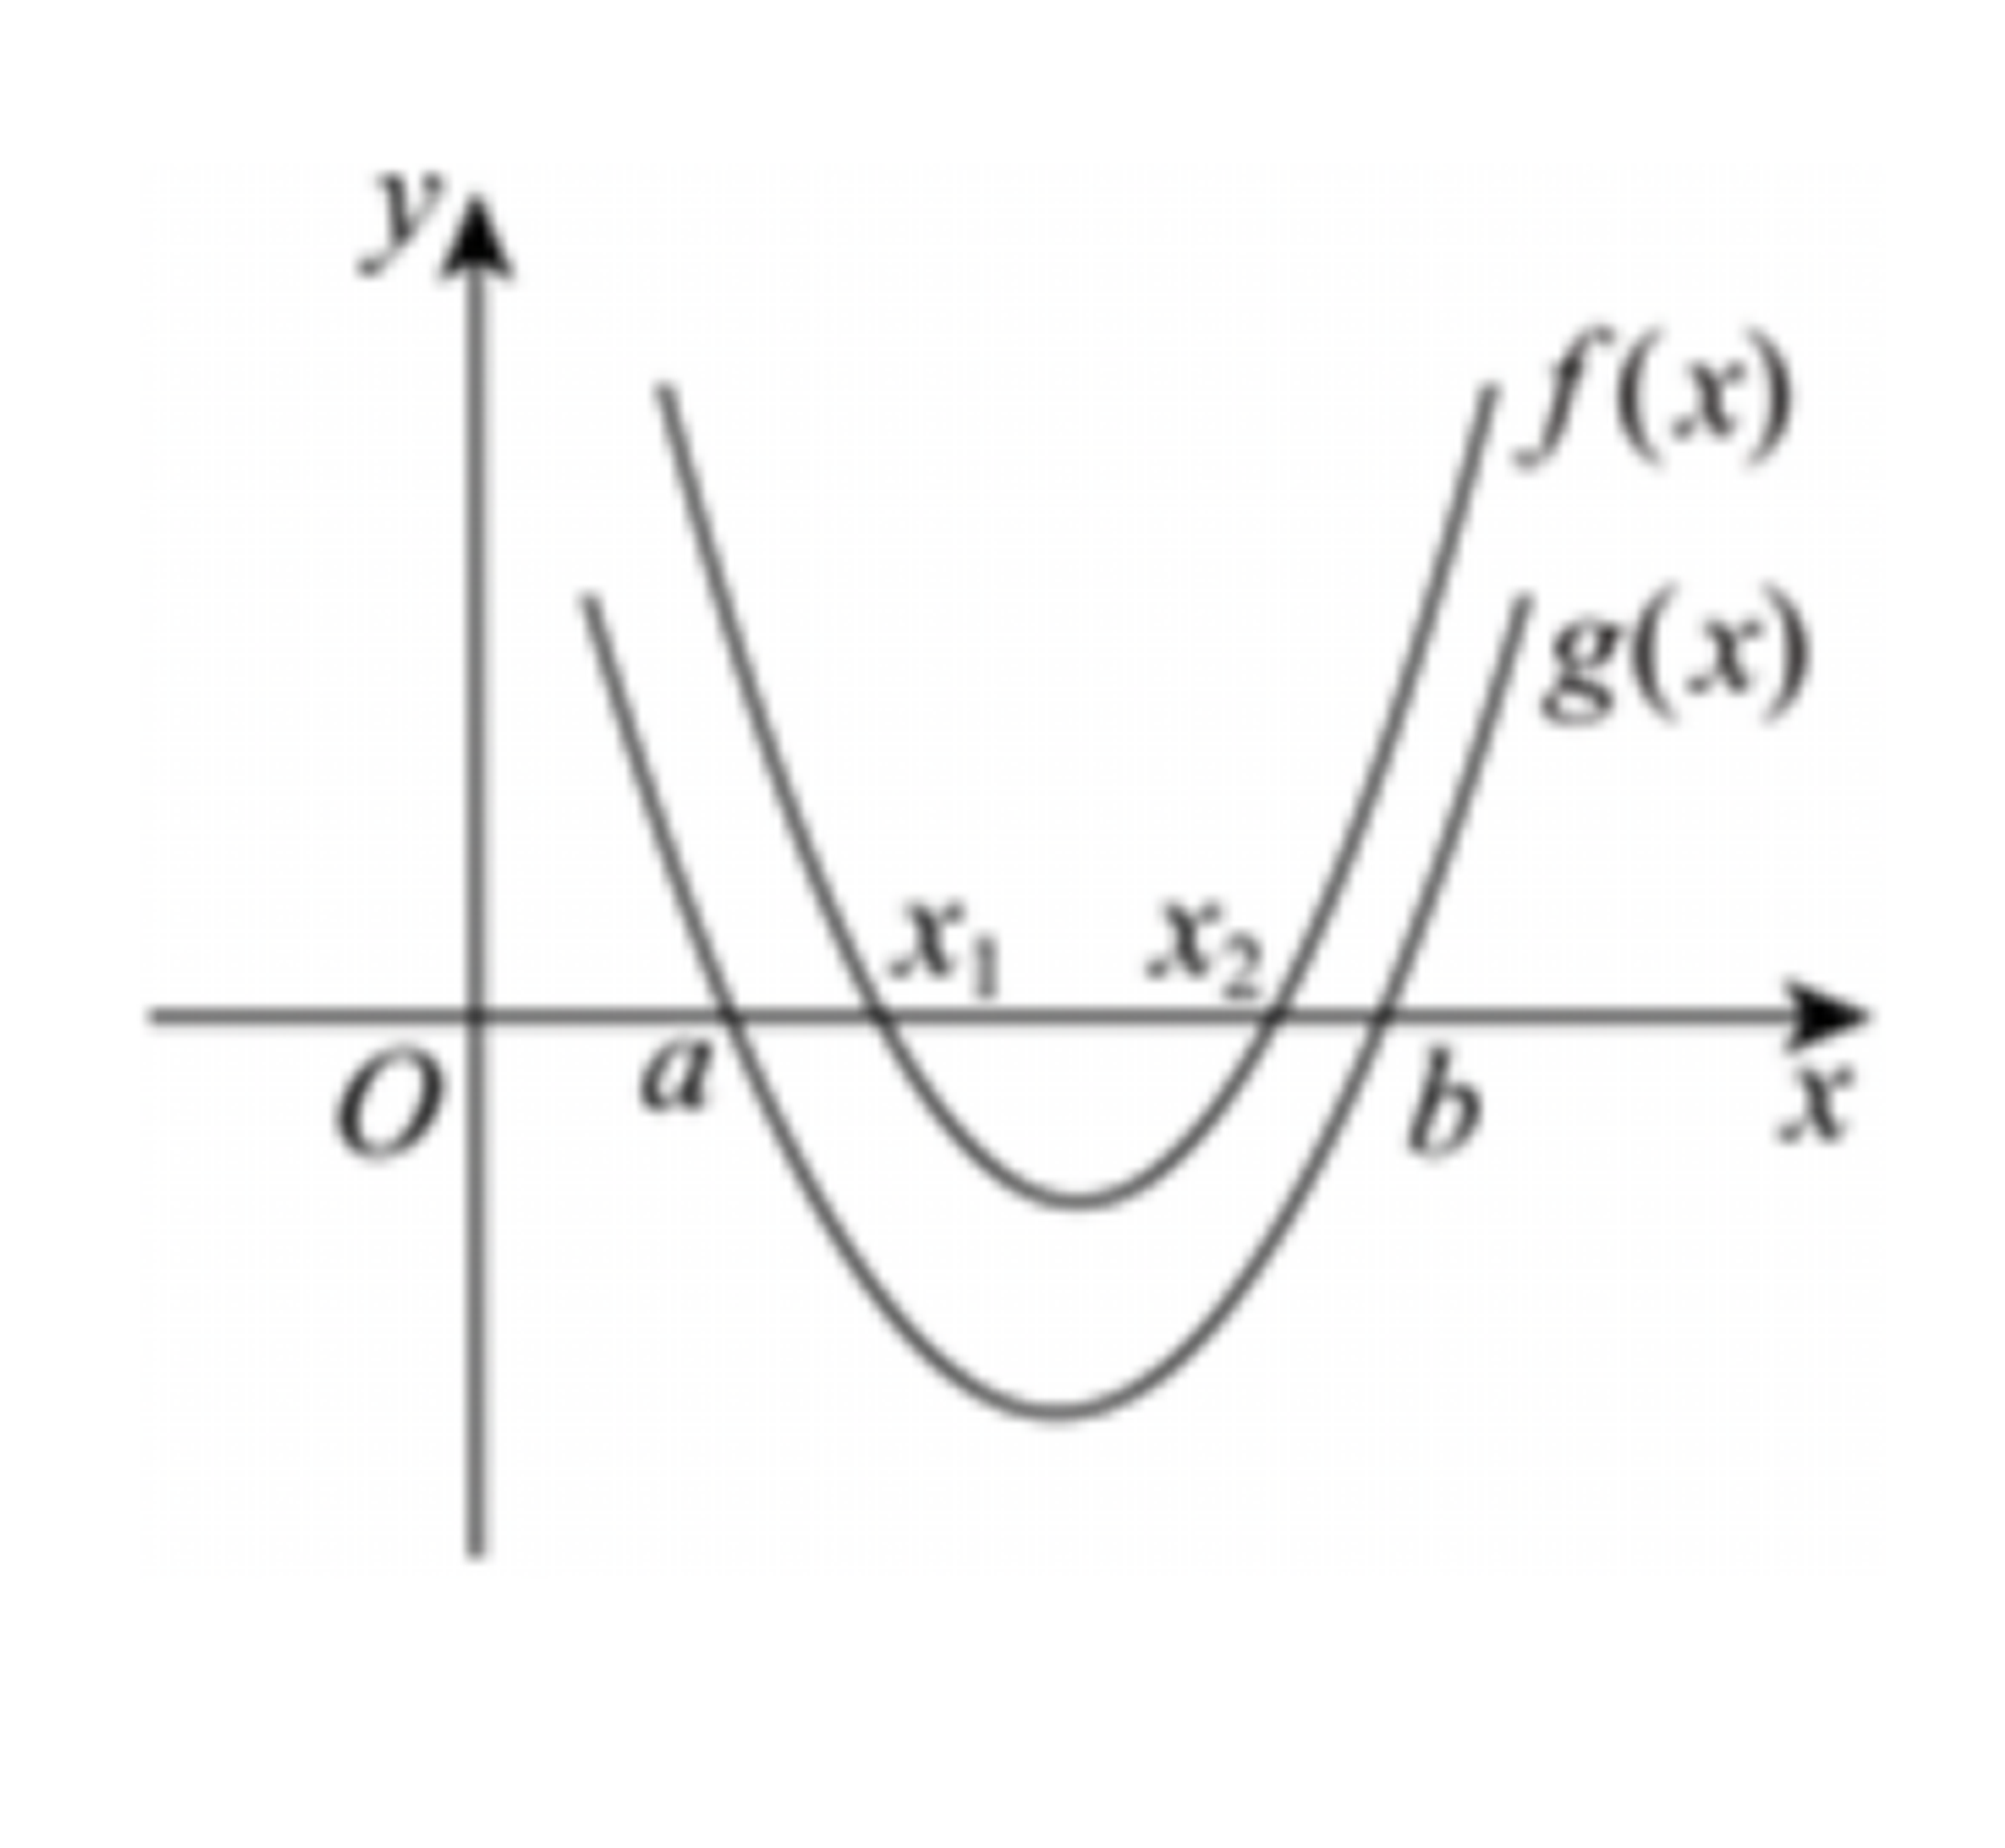
\includegraphics[width=0.30\textwidth]{figures/parabola_f_g_x1x2_h65.png}
\end{center}
\step{由图像得 $a<x_1<x_2<b$，故选 $B$.}
\solend
\fi

\end{enumerate}

\bigsec{三、解答题}

\begin{enumerate}
\setcounter{enumi}{16}

\item 已知 $a>0$，$b>0$，若 $a+b>4$，求证：$\dfrac a{b+2}$ 和 $\dfrac b{a+2}$ 中至少有一个大于 $\dfrac12$.

\ifanswer
\solbegin
\step{假设 $\dfrac a{b+2}\leqslant\dfrac12$，$\dfrac b{a+2}\leqslant\dfrac12$，}
\step{$a>0$，$b>0$，则 $a+2>0$，$b+2>0$，故 $2a\leqslant b+2$，$2b\leqslant a+2$，}
\step{两式相加得 $a+b\leqslant4$，与 $a+b>4$ 矛盾，故 $\dfrac a{b+2}$ 和 $\dfrac b{a+2}$ 中至少有一个大于 $\dfrac12$.}
\solend
\fi

\ansspace[6]

\item 已知集合 $A=\{x\mid-4<x<5\}$，$B=\{x\mid x\leqslant a-6\text{ 或 }x\geqslant a+2\}$.

\begin{enumerate}[label=(\arabic*)]

\item 若 $A\cup B=\R$，求实数 $a$ 的取值范围；

\item 若“$x\in A$”是“$x\in B$”的充分不必要条件，求实数 $a$ 的取值范围.

\end{enumerate}

\ifanswer
\solbegin
\stepm{(1)}{集合 $A=\{x\mid-4<x<5\}$，$B=\{x\mid x\leqslant a-6\text{ 或 }x\geqslant a+2\}$.}
\step{由 $A\cup B=\R$ 得 $\begin{cases}a-6\geqslant-4\\ a+2\leqslant5\end{cases}$，解得 $2\leqslant a\leqslant3$，$a$ 的取值范围为 $[2,3]$；}
\stepm{(2)}{若“$x\in A$”是“$x\in B$”的充分不必要条件，则 $A\subset B$，}
\step{则 $5\leqslant a-6$ 或 $-4\geqslant a+2$，解得 $a\leqslant-6$ 或 $a\geqslant11$.}
\solend
\fi

\ansspace[8]

% 注：原卷题干把命题 $P$ 印作“$\exists3\notin A$”（多一个存在量词），而【解析】两处均作
%     “$3\notin A$”；照录未改，见文件头“原卷笔误/存疑”③。
\item 已知集合 $A=\left\{x\mid\dfrac{x-1}{x-m}<0\right\}$，集合 $B=\left\{x\mid\left|\dfrac{x-1}{x-3}\right|\geqslant1\right\}$，命题 $P$：“$\exists3\notin A$”，命题
$Q$：$A\cap B\neq\varnothing$.

\begin{enumerate}[label=(\arabic*)]

\item 若命题 $P$ 为真命题，求 $m$ 的取值范围；

\item 若命题 $P$ 和命题 $Q$ 至少有一个为假命题，求实数 $m$ 的取值范围.

\end{enumerate}

\ifanswer
\solbegin
\stepm{(1)}{$A=\left\{x\mid\dfrac{x-1}{x-m}<0\right\}=\{x\mid(x-1)(x-m)<0\}$，}
\step{若命题 $P$：“$3\notin A$”为真命题，则 $(3-1)(3-m)\geqslant0$，解得 $m\leqslant3$，}
\step{故实数 $m$ 的取值范围为 $(-\infty,3]$；}
\stepm{(2)}{$B=\left\{x\mid\left|\dfrac{x-1}{x-3}\right|\geqslant1\right\}$，由 $\left|\dfrac{x-1}{x-3}\right|\geqslant1$，得 $\begin{cases}|x-1|\geqslant|x-3|\\ x\neq3\end{cases}$，}
\step{等价于 $\begin{cases}(x-1)^2\geqslant(x-3)^2\\ x\neq3\end{cases}$，解得 $x\geqslant2$ 且 $x\neq3$，所以 $B=[2,3)\cup(3,+\infty)$，}
\step{因为 $A=\{x\mid(x-1)(x-m)<0\}$，}
\step{当 $m=1$ 时，$A=\varnothing$，不满足 $A\cap B\neq\varnothing$，}
\step{当 $m<1$ 时，$A=(m,1)$，不满足 $A\cap B\neq\varnothing$，}
\step{当 $m>1$ 时，$A=(1,m)$，要使 $A\cap B\neq\varnothing$，则 $m>2$，}
\step{则若命题 $Q$：“$A\cap B\neq\varnothing$”为真命题时，实数 $m$ 的取值范围为 $(2,+\infty)$，}
\step{当命题 $P$ 与命题 $Q$ 都是真命题时，则 $\begin{cases}m\leqslant3\\ m>2\end{cases}$，解得 $2<m\leqslant3$，}
\step{则命题 $P$ 和命题 $Q$ 至少有一个为假命题时，得 $m\leqslant2$ 或 $m>3$，}
\step{故实数 $m$ 的取值范围为 $(-\infty,2]\cup(3,+\infty)$.}
\solend
\fi

\ansspace[8]

\item 已知函数 $y=ax^2-(a+2)x+2$，$a\in\R$.

\begin{enumerate}[label=(\arabic*)]

\item $y<3-2x$ 恒成立，求实数 $a$ 的取值范围；

% 注：原卷末句作“求实数 $a$ 的取值”（疑脱“范围”二字），照录未改，
%     见文件头“原卷笔误/存疑”⑤。
\item 若存在 $m>0$ 使关于 $x$ 的方程 $ax^2-(a+2)|x|+2=m+\dfrac1m+1$ 有四个不同的实根，
求实数 $a$ 的取值.

\end{enumerate}

\ifanswer
\solbegin
\stepm{(1)}{由题意得 $ax^2-(a+2)x+2<3-2x$ 恒成立，}
\step{即 $ax^2-ax-1<0$ 恒成立，}
\step{当 $a=0$ 时，$-1<0$ 恒成立，符合题意，}
\step{当 $a\neq0$ 时，则 $\begin{cases}a<0\\ \triangle=a^2+4a<0\end{cases}$，得 $\begin{cases}a<0\\ -4<a<0\end{cases}$，得 $-4<a<0$，}
\step{综上，$a$ 的取值范围为 $(-4,0]$.}
\stepm{(2)}{当 $m>0$ 时，令 $t=m+\dfrac1m+1\geqslant2\sqrt{m\times\dfrac1m}+1=3$，}
\step{当且仅当 $m=1$ 时取等号，}
% 注：题干只给“函数 $y=ax^2-(a+2)x+2$”，全卷未设 $f$，此处 $f(|x|)$ 无定义；
%     照录未改，见文件头“原卷笔误/存疑”④。
\step{则关于 $x$ 的方程 $f(|x|)=t$ 可化为 $a|x|^2-(a+2)|x|+2-t=0$，}
\step{关于 $x$ 的方程为 $a|x|^2-(a+2)|x|+2-t=0$ 有四个不等的实数根，}
\step{即 $ax^2-(a+2)x+2-t=0$，有两个不同的实数正根，}
\step{则 $\begin{cases}\triangle=(a+2)^2-4a(2-t)>0\\ \dfrac{a+2}a>0\\ \dfrac{2-t}a>0\end{cases}$，解得 $a<-2$，}
\step{由（1）得存在 $t\in[3,+\infty)$ 使得不等式 $4at+(a+2)^2-8a>0$ 成立，}
\step{故 $4a\times3+(a+2)^2-8a>0$，即 $a^2+8a+4>0$，}
\step{解得 $a<-4-2\sqrt3$ 或 $a>-4+2\sqrt3$，}
\step{综上，$a<-4-2\sqrt3$，所以 $a$ 的取值范围为 $(-\infty,-4-2\sqrt3)$.}
\solend
\fi

\ansspace[8]

\item 若集合 $A=B_1\cup B_2\cup\cdots\cup B_n$，其中 $B_1$、$B_2$、$\cdots$、$B_n$ 为非空集合，
$B_i\cap B_j=\varnothing$($1\leqslant i<j\leqslant n$)，则称集合 $\{B_1,B_2,\cdots,B_n\}$ 为集合 $A$ 的一个 $n$ 划分.

\begin{enumerate}[label=(\arabic*)]

\item 写出集合 $A=\{1,2,3\}$ 的所有不同的 2 划分；

\item 设 $\{B_1,B_2\}$ 为有理数集 $\Q$ 的一个 2 划分，且满足对任意 $x\in B_1$，任意 $y\in B_2$，都有
$x<y$，判断命题“$B_1$ 中的元素存在最大值，$B_2$ 中的元素存在最小值.”的真假，并说明
理由.

\item 设集合 $A=\{1,2,3,\cdots,16\}$，对于集合 $A$ 的任意一个 3 划分 $\{B_1,B_2,B_3\}$，判断是否存
在 $i\in\{1,2,3\}$，存在 $a$、$b\in B_i$，使得 $b-a\in B_i$ 成立，并说明理由.

\end{enumerate}

\ifanswer
\solbegin
% 注：原卷三个“2 划分”本有外层花括号（$\{\{1,2\},\{3\}\}$ 等），首轮误脱；
%     第二轮复核照原卷补回（原卷原样 / 本稿原错处：原脱外层花括号）。
\stepm{(1)}{集合 $A=\{1,2,3\}$ 的所有不同的 2 划分为 $\{\{1,2\},\{3\}\}$、$\{\{1,3\},\{2\}\}$、}
\step{$\{\{2,3\},\{1\}\}$.}
\stepm{(2)}{该命题为假命题，理由如下：}
\step{假设命题为真，则不妨设 $B_1$ 中元素的最大值为 $s$，$B_2$ 中元素的最小值为 $t$，}
\step{由题意得 $s<t$，所以 $s<\dfrac{s+t}2<t$，}
\step{因为 $s$ 为 $B_1$ 中元素的最大值，所以 $\dfrac{s+t}2\notin B_1$，}
\step{因为 $t$ 为 $B_2$ 中元素的最小值，所以 $\dfrac{s+t}2\notin B_2$，}
\step{因为 $B_1\cup B_2=\Q$，所以 $\dfrac{s+t}2\notin\Q$，}
\step{这与 $\dfrac{s+t}2\in\Q$ 矛盾，所以假设不成立，即命题不可能成立；}
\stepm{(3)}{由于集合 $A$ 中有 16 个元素，}
\step{所以 $B_1$、$B_2$、$B_3$ 中至少有一个集合至少包含 6 个元素，}
\step{不妨设 $B_1$ 中至少包含 6 个元素，}
\step{设 $b_1$、$b_2$、$b_3$、$b_4$、$b_5$、$b_6\in B_1$，且 $b_1<b_2<b_3<b_4<b_5<b_6$，}
\step{假设对任意 $i\in\{1,2,3\}$，对任意 $a$、$b\in B_i$，都有 $b-a\notin B_i$，}
\step{那么 $b_6-b_1$、$b_6-b_2$、$b_6-b_3$、$b_6-b_4$、$b_6-b_5\notin B_1$，}
\step{又因为 $b_6-b_1$、$b_6-b_2$、$b_6-b_3$、$b_6-b_4$、$b_6-b_5\in A$，}
\step{所以 $b_6-b_1$、$b_6-b_2$、$b_6-b_3$、$b_6-b_4$、$b_6-b_5\in B_2\cup B_3$，}
\step{则 $B_2$、$B_3$ 中必有一个集合}
\step{至少包含 $b_6-b_1$、$b_6-b_2$、$b_6-b_3$、$b_6-b_4$、$b_6-b_5$ 中的 3 个元素，}
\step{不妨设这 3 个元素为 $a_1$、$a_2$、$a_3\in B_2$，$a_1<a_2<a_3$，}
\step{由假设得 $a_3-a_1$、$a_3-a_2$、$a_2-a_1\notin B_2$，}
\step{对任意 $i$、$j$($1\leqslant j<i\leqslant3$)，存在 $m$、$n$($1\leqslant m<n\leqslant5$)，}
\step{都有 $a_i-a_j=b_6-b_m-b_6+b_n=b_n-b_m\notin B_1$，}
\step{又因为 $a_3-a_1$、$a_3-a_2$、$a_2-a_1\in B_3$，而 $a_3-a_1-(a_3-a_2)=a_2-a_1$，}
\step{与假设矛盾，所以假设不成立，}
\step{即存在 $i\in\{1,2,3\}$，存在 $a$、$b\in B_i$，使得 $b-a\in B_i$.}
\solend
\fi

\ansspace*[10]

\end{enumerate}

\end{document}
"
%
% 原始材料：微信公众号“魔都数学加油站”文章，作者破晓，连载“27学年高一65”；
% 原文标题“27学年高一65——2026-2027年上海市大同中学高一上10月月考”；
% 原文链接：https://mp.weixin.qq.com/s/h9ctuk-ByE1Vfg2Rx2C6bw。
% 页面标注发布时间 2026-10-17 21:58（上海）。
% 本次转录只据 `原图/高一65_大同中学_10月月考/` 的 11 张 PNG 逐页读图。
% 正文为 11 张 PNG 页（`01..11.png`）：
% 第 06、11 页 2560×3620，第 01、02、03、04、05、07、08、09、10 页 4762×6735
% （**同一篇各页分辨率不同**），均按页序读取。11 页全为试卷正文页（卷首标题在第 1 页页顶，
% 卷末解答题第 21 题解析止于第 11 页），无封面页、目录页、二维码或宣传页。
% 粉色斜排“魔都数学加油站”为卷面水印，与公众号页脚一并未录入。
%
% 卷首标题：照卷面印作“2026--2027 年大同中学高一上 10 月月考”，年份区间按全稿惯例排 en dash。
% 原卷只有一行标题、无副标题。
%
% 篇幅与题号：原卷自第 3 题起编号（第 1、2 题不在本卷内）。填空题 3—12（10 题）、
% 选择题 13—16（4 题）、解答题 17—21（5 题），共 19 题。本稿沿用原节与原题号，
% 只改排为全稿统一的大节样式（原卷小节标题为“一、填空题”“二、选择题”“三、解答题”）。
%
% 讲评版：原卷每题下直接印【答案】或【解析】。**只印【答案】的 4 题**（第 3、4、7、10 题），
% 本稿只给 \ans{}；其余 15 题都印【解析】（按全稿口径这类题不另提 \ans{}——第 12、13、14、
% 15、16 题的结论写在解析末句（“故选 B”“综上，n 的最大值为 14”等），亦照录在解析内）。
% 全卷无“答案印在题干括号内”的题（第 13—16 题的选择题括号内均空白）。
%
% 副标题：原卷未印副标题。本稿按“知识模块”口径标作“集合与常用逻辑用语、不等式”：
% 19 题中集合与常用逻辑用语 10 题（第 3、4、6、8、12、14、15、18、19、21 题），
% 不等式 9 题（含等式恒等、不等式性质、二次不等式、恒成立、基本不等式、不等式的证明：
% 第 5、7、9、10、11、13、16、17、20 题），两类均超过三分之一，故并标。口径同 高一63。
%
% 与原卷的排版差异：
%   ① 原卷每题下直接印【答案】/【解析】，本稿按全稿惯例将答案与解析置于答案版，试卷版保持干净；
%   ② 原卷未印副标题，本稿按“知识模块”口径补出；
%   ③ 原卷填空横线约四个字宽，本稿按全稿惯例统一排 \blankline[4.4em]；
%   ④ 原卷数集记号全为斜体：实数集作 $R$（第 6 题两处、第 8 题两处、第 15 题解析、第 18 题、
%      第 20 题题干），自然数集作 $N$（第 12 题题干“$n\in N,n\geqslant1$”），有理数集作 $Q$
%      （第 21 题 (2) 题干与解析共 4 处），本稿按全稿惯例统一改用 $\R$、$\N$、$\Q$
%      （同 高一63 排版差异④：记号归一）；空集记号原卷作 $\varnothing$，照录；
%   ⑤ 原卷用描述法时竖线排细竖“$|$”（如 $\{x|0<x<3\}$、$\{x|(x-1)(x-m)<0\}$），
%      本稿按全稿惯例排 \mid；
%   ⑥ 原卷判别式印作“$\triangle$”（第 8、14 题解析各 1 处、第 20 题解析 2 处，共 4 处），
%      本稿照录用 \triangle（同 高一39 成例），未改作 \Delta；
%   ⑦ 第 18—21 题的子问原卷各自另起一行、以“（1）”“（2）”标号，本稿按全稿惯例用
%      enumerate 的 (1)(2)(3)；解析中的子问标号一律用 \stepm{(1)}{…}；
%      第 18—21 题解析（原文以“（1）”“（2）”“（3）”冠于解析首句）同此；
%   ⑧ 选择题的作答括号原卷排半角“(　　)”（第 13—16 题括号内均空白），
%      本稿按全稿惯例排 \mbox{（\quad）}；选项字母后的句点照原卷排“A.”“B.”；
%   ⑨ 每道解答题原卷未留作答空白，本稿按全稿惯例加 \ansspace（末题用 \ansspace*）；
%   ⑩ 原卷在数学式内多处用半角逗号（如 $\{x|0<x<3\},B=\{x|x>2\}$、$m\in I_{14},k\in I_{14}$），
%      均照录未强改；句末句点按全稿惯例排西文句点。
%
% 原卷笔误/存疑（均照录未改，正文对应处另有 % 注）：
%   ① 第 13 题题干“下列不等式中一定成立是（　　）”脱一个“的”（当作“一定成立的是”），
%      8 倍放大确认非水印遮挡，本稿照录；
%   ② 第 15 题【解析】末段把题干条件“$x\geqslant10$”写成“$x\geqslant1$”
%      （“所以 $x+2+\frac{16}{x+2}(x\geqslant1)$ 的最小值不为 8”），与同段前面“令 $t=x+2$，
%      则 $t\geqslant12$”不合，本稿照录；
%   ③ 第 19 题题干把命题 $P$ 印作“$\exists3\notin A$”（多一个存在量词），而【解析】两处
%      均作“$3\notin A$”，前后记号不一，本稿照录；
%   ④ 第 20 题【解析】(2) 出现 $f(|x|)$，但题干只给“函数 $y=ax^2-(a+2)x+2$”、全卷未设 $f$，
%      本稿照录；
%   ⑤ 第 20 题 (2) 题干末句作“求实数 $a$ 的取值”（疑脱“范围”二字），本稿照录；
%   ⑥ 第 12 题【解析】第 18 步“它与 $P_n$ 中的任何其他数之和都不是整数”，该段所论为 $P_{14}$
%      （前后均作 $P_{14}$），此处 $P_n$ 疑当作 $P_{14}$，本稿照录。
%
% 第二轮复核（2026-10-18）订正「本稿抄错原卷」一处：
%   第 21 题 (1)【解析】原卷本作“$\{\{1,2\},\{3\}\}$、$\{\{1,3\},\{2\}\}$、$\{\{2,3\},\{1\}\}$”，
%   有外层花括号；首轮误脱外层花括号，并曾在文件头误记为“原卷未加外层花括号”（原第 ⑦ 条，
%   已撤销）。本次照原卷补回，正文对应处另有 % 注。
%
% 插图：第 16 题【解析】内有 1 幅图（两条开口向上的抛物线 $f(x)$、$g(x)$ 与 $x$ 轴交点
% 标 $a$、$x_1$、$x_2$、$b$，纵轴标 $y$、原点 $O$），解析第三行“画出函数 $g(x)$ 与函数 $f(x)$
% 的图像，如图所示”即指此图；取原卷截图（06.png，2560×3620）右半幅，4× LANCZOS 放大，
% 存 figures/parabola_f_g_x1x2_h65.png。该图在【解析】内，仅答案版出。
%
\documentclass[a4paper,11pt]{article}
\usepackage{common}

\begin{document}

\examtitlest[3]{2026--2027 年大同中学高一上 10 月月考}{集合与常用逻辑用语、不等式}

\bigsec{一、填空题}

\begin{enumerate}
\setcounter{enumi}{2}

\item 已知集合 $A=\{x\mid0<x<3\}$,$B=\{x\mid x>2\}$，则集合 $A\cup B=$\blankline[4.4em].

\ifanswer
\ans{$(0,+\infty)$}
\fi

\item “$x>1$ 或 $y>1$”的否定形式是\blankline[4.4em].

\ifanswer
\ans{$x\leqslant1$ 且 $y\leqslant1$}
\fi

\item 已知等式 $2x^2+3x+4=a(2x+1)(x+1)+b$ 恒成立，则常数 $a-b=$\blankline[4.4em].

\ifanswer
\solbegin
\step{因为等式 $2x^2+3x+4=a(2x+1)(x+1)+b$ 恒成立，}
\step{所以 $a(2x+1)(x+1)+b=2ax^2+3ax+a+b=2x^2+3x+4$，}
\step{所以 $\begin{cases}2a=2\\ 3a=3\\ a+b=4\end{cases}$，解得 $\begin{cases}a=1\\ b=3\end{cases}$，所以 $a-b=-2$.}
\solend
\fi

\item 全集为 $U=\R$，$A=\{x\mid|x|\geqslant2\}$，$B=\{y\mid y=x^2+1,x\in\R\}$，则 $A\cup\bar B=$\blankline[4.4em].

\ifanswer
\solbegin
\step{由题意得集合 $A=\{x\mid x\geqslant2\text{ 或 }x\leqslant-2\}$，}
\step{因为 $x^2+1\geqslant1$，所以集合 $B=\{x\mid x\geqslant1\}$，所以 $\bar B=\{x\mid x<1\}$，}
\step{则 $A\cup\bar B=\{x\mid x\geqslant2\text{ 或 }x<1\}$.}
\solend
\fi

\item 已知 $|x+3|+|x-5|=8$，则实数 $x$ 的取值范围为\blankline[4.4em].

\ifanswer
\ans{$[-3,5]$}
\fi

\item 已知集合 $A=\{x\in\R\mid ax^2+2x+1=0,a\in\R\}$ 只有一个元素，则 $a$ 的值为\blankline[4.4em].

\ifanswer
\solbegin
\step{当 $a=0$ 时，$A=\left\{-\dfrac12\right\}$；}
\step{当 $a\neq0$ 时，若集合 $A$ 只有一个元素，由 $\triangle=4-4a=0$ 得 $a=1$.}
\step{综上，当 $a=0$ 或 $a=1$ 时，集合 $A$ 只有一个元素.}
\solend
\fi

\item 已知不等式 $-x^2+bx+c>0$ 的解集为 $(3,4)$，则不等式 $cx^2+bx-1<0$ 的解集为\blankline[4.4em].

\ifanswer
\solbegin
\step{由题意得 3，4 是方程 $-x^2+bx+c=0$ 的两个实数根，}
\step{所以 $\begin{cases}3+4=b\\ 3\times4=-c\end{cases}$，得 $b=7$，$c=-12$，}
\step{则不等式 $cx^2+bx-1<0$，即为 $-12x^2+7x-1<0$，即 $12x^2-7x+1>0$，}
\step{化简得 $(3x-1)(4x-1)>0$，解得 $x<\dfrac14$ 或 $x>\dfrac13$，}
\step{即不等式 $cx^2+bx-1<0$ 的解集为 $\left(-\infty,\dfrac14\right)\cup\left(\dfrac13,+\infty\right)$.}
\solend
\fi

\item 对于区间 $(m,n)$，我们将 $n-m$ 的值称为该区间的长度. 若关于 $x$ 的不等式
$x^2+ax+a<0$ 有解，且解集的区间长度不超过 $2\sqrt3$，则实数 $a$ 的取值范围是\blankline[4.4em].

\ifanswer
\ans{$[-2,0)\cup(4,6]$}
\fi

\item 当 $x>0$ 时，关于 $x$ 的不等式 $(ax-1)(x^2+bx-4)\geqslant0$ 恒成立，则 $b+\dfrac2a$ 的最小值
为\blankline[4.4em].

\ifanswer
\solbegin
\step{由题意 $a\neq0$；}
\step{若 $a<0$，则 $x>0$ 时 $ax-1<0$ 恒成立，需 $x^2+bx-4\leqslant0$ 对一切 $x>0$ 成立，}
\step{而 $y=x^2+bx-4$ 的图象开口向上，当 $x$ 充分大时必为正值，矛盾，故 $a>0$.}
\step{当 $a>0$ 时，$ax-1=a\left(x-\dfrac1a\right)$，故原条件化为 $\left(x-\dfrac1a\right)(x^2+bx-4)\geqslant0$：}
\step{若 $0<x<\dfrac1a$，则 $x-\dfrac1a<0$，需 $x^2+bx-4\leqslant0$；}
\step{若 $x>\dfrac1a$，则 $x-\dfrac1a>0$，需 $x^2+bx-4\geqslant0$；}
\step{由 $y=x^2+bx-4$ 的连续性知 $x=\dfrac1a$ 是它的零点，}
\step{即 $\dfrac1{a^2}+\dfrac ba-4=0$，得 $b=4a-\dfrac1a$；}
\step{此时 $x^2+bx-4=x^2+\left(4a-\dfrac1a\right)x-4=(x+4a)\left(x-\dfrac1a\right)$，}
\step{由 $a>0$、$x>0$ 得 $x+4a>0$，}
\step{其符号与 $x-\dfrac1a$ 一致，故能与 $ax-1$ 同号，原不等式确在 $x>0$ 上恒成立.}
\step{于是 $b+\dfrac2a=4a-\dfrac1a+\dfrac2a=4a+\dfrac1a\geqslant2\sqrt{4a\cdot\dfrac1a}=4$，}
\step{当且仅当 $a=\dfrac12$ 时取等号，故最小值为 4.}
\solend
\fi

\item 设集合 $I_n=\{1,2,\cdots,n\}$，$n\in\N$，$n\geqslant1$，集合 $P_n=\left\{\dfrac m{\sqrt k}\mid m\in I_n,k\in I_n\right\}$，若 $P_n$ 的子集 $A$
中任意两个元素之和不是整数的平方，则称 $A$ 为“人文集”. 那么使 $P_n$ 能分成两个交集为空
集的“人文集”的并集，且这两个人文集的并集恰为 $P_n$ 时，$n$ 的最大值是\blankline[4.4em].

\ifanswer
\solbegin
\step{先证当 $n\geqslant15$ 时，$P_n$ 不能分成两个不相交的人文集的并集.}
\step{假设当 $n\geqslant15$ 时，$P_n$ 可以分成两个不相交的人文集的并集，}
\step{设 $A$ 和 $B$ 为两个不相交的人文集，使 $A\cup B=P_n\supseteq I_n$.}
\step{不妨设 $1\in A$，则由于 $1+3=2^2$，所以 $3\notin A$，即 $3\in B$.}
\step{同理可得，$6\in A$，$10\in B$. 又推出 $15\in A$，}
\step{但 $1+15=4^2$，这与 $A$ 为人文集相矛盾.}
\step{再证 $P_{14}$ 满足要求. 当 $k=1$ 时，$P_{14}=\left\{\dfrac m{\sqrt k}\mid m\in I_{14},k\in I_{14}\right\}$，}
\step{可以分成 2 个人文集的并集.}
\step{事实上，只要取 $A_1=\{1,2,4,6,9,11,13\}$，$B_1=\{3,5,7,8,10,12,14\}$，}
\step{则 $A_1$ 和 $B_1$ 都是人文集，且 $A_1\cup B_1=P_{14}$.}
\step{当 $k=4$ 时，集合 $\left\{\dfrac m{\sqrt k}\mid m\in I_{14}\right\}$ 中，除整数外，}
\step{剩下的数组成集合 $\left\{\dfrac12,\dfrac32,\dfrac52,\cdots,\dfrac{13}2\right\}$，}
\step{可以分为下列 2 个人文集的并：$A_2=\left\{\dfrac12,\dfrac52,\dfrac92,\dfrac{11}2\right\}$，$B_2=\left\{\dfrac32,\dfrac72,\dfrac{13}2\right\}$.}
\step{当 $k=9$ 时，集合 $\left\{\dfrac m{\sqrt k}\mid m\in I_{14}\right\}$ 中，除整数外，}
\step{剩下的数组成集合 $\left\{\dfrac13,\dfrac23,\dfrac43,\dfrac53,\cdots,\dfrac{13}3,\dfrac{14}3\right\}$，}
\step{可以分为下列 2 个人文集的并：$A_3=\left\{\dfrac13,\dfrac43,\dfrac53,\dfrac{10}3,\dfrac{13}3\right\}$，$B_3=\left\{\dfrac23,\dfrac73,\dfrac83,\dfrac{11}3,\dfrac{14}3\right\}$.}
\step{最后，集合 $C=\left\{\dfrac m{\sqrt k}\mid m\in I_{14},k\in I_{14},k\neq1,4,9\right\}$ 中的数的分母都是无理数，}
% 注：本行原卷作“$P_n$”，而该段所论为 $P_{14}$（前后均作 $P_{14}$），疑当作 $P_{14}$；
%     照录未改，见文件头“原卷笔误/存疑”⑥。
\step{它与 $P_n$ 中的任何其他数之和都不是整数，}
\step{因此，令 $A=A_1\cup A_2\cup A_3\cup C$，$B=B_1\cup B_2\cup B_3$，}
\step{则 $A$ 和 $B$ 是不相交的人文集，且 $A\cup B=P_{14}$.}
\step{综上，$n$ 的最大值为 14.}
\solend
\fi

\end{enumerate}

\bigsec{二、选择题}

\begin{enumerate}
\setcounter{enumi}{12}

% 注：原卷题干“下列不等式中一定成立是”脱一个“的”（当作“一定成立的是”），
%     照录未改，见文件头“原卷笔误/存疑”①。
\item 已知 $a>b$，下列不等式中一定成立是\mbox{（\quad）}

\keepwithprev
A. $a^2>b^2$\qquad B. $ac^2>bc^2$\qquad C. $\dfrac1a<\dfrac1b$\qquad D. $a+3>b-4$

\ifanswer
\solbegin
\step{对于 $A$，当 $a=-2$，$b=-4$ 时，不等式不成立，故 $A$ 错误；}
\step{对于 $B$，当 $c=0$ 时，不等式不成立，故 $B$ 错误；}
\step{对于 $C$，当 $a=2$，$b=-4$ 时，不等式不成立，故 $C$ 错误；}
\step{对于 $D$，因为 $a>b$，$3>-4$，必有 $a+3>b-4$ 成立，故 $D$ 正确.}
\step{故选 $D$.}
\solend
\fi

\item 已知 $a$ 为实数，那么“$|a|\leqslant2$”是“方程 $x^2+ax+1=0$ 没有实数解”的\mbox{（\quad）}

\keepwithprev
A. 充分而不必要条件\qquad B. 必要而不充分条件

C. 充要条件\qquad D. 既不充分也不必要条件

\ifanswer
\solbegin
\step{由方程 $x^2+ax+1=0$ 没有实数解，得 $\triangle=a^2-4<0$，则 $|a|<2$，}
\step{由 $|a|<2$ 得 $|a|\leqslant2$，反之不成立，}
\step{所以“$|a|\leqslant2$”是“方程 $x^2+ax+1=0$ 没有实数解”的必要而不充分条件.}
\step{故选 $B$.}
\solend
\fi

\item 下列命题为真命题的是\mbox{（\quad）}

\keepwithprev
A. $a>b>0$，当 $m>0$ 时，$\dfrac{a+m}{b+m}>\dfrac ab$

B. 集合 $A=\{x\mid y=x^2+1\}$ 与集合 $B=\{y\mid y=x^2+1\}$ 是相同的集合

C. 若 $b<a<0$，$m<0$，则 $\dfrac ma>\dfrac mb$

D. $x+2+\dfrac{16}{x+2}(x\geqslant10)$ 最小值为 8

\ifanswer
\solbegin
\step{对于 $A$，$\dfrac{a+m}{b+m}-\dfrac ab=\dfrac{b(a+m)-a(b+m)}{b(b+m)}=\dfrac{m(b-a)}{b(b+m)}$，}
\step{因为 $a>b>0$，$m>0$，所以 $b(b+m)>0$，$m(b-a)<0$，}
\step{所以 $\dfrac{a+m}{b+m}-\dfrac ab=\dfrac{m(b-a)}{b(b+m)}<0$，}
\step{即 $a>b>0$，当 $m>0$ 时，$\dfrac{a+m}{b+m}<\dfrac ab$，故 $A$ 错误；}
\step{对于 $B$，集合 $A=\{x\mid y=x^2+1\}=\R$，集合 $B=\{y\mid y=x^2+1\}=\{y\mid y\geqslant1\}$，}
\step{所以 $A\neq B$，故 $B$ 错误；}
\step{对于 $C$，$\dfrac ma-\dfrac mb=\dfrac{m(b-a)}{ab}$，}
\step{因为 $b<a<0$，$m<0$，所以 $ab>0$，$m(b-a)>0$，}
\step{所以 $\dfrac ma-\dfrac mb=\dfrac{m(b-a)}{ab}>0$，即 $\dfrac ma>\dfrac mb$，故 $C$ 正确；}
\step{对于 $D$，令 $t=x+2$，则 $t\geqslant12$，表达式变为 $t+\dfrac{16}t$，}
\step{$t+\dfrac{16}t\geqslant2\sqrt{t\cdot\dfrac{16}t}=8$，当且仅当 $t=4$ 时取等号，即等号不成立，}
% 注：原卷本行把题干条件“$x\geqslant10$”写成“$x\geqslant1$”，与同段“$t\geqslant12$”不合；
%     照录未改，见文件头“原卷笔误/存疑”②。
\step{所以 $x+2+\dfrac{16}{x+2}(x\geqslant1)$ 的最小值不为 8，故 $D$ 错误.}
\step{故选 $C$.}
\solend
\fi

\item 已知实数 $a<b$，关于 $x$ 的不等式 $x^2-(a+b)x+ab+\dfrac12<0$ 的解集为 $(x_1,x_2)$，则实数 $a$、
$b$、$x_1$、$x_2$ 从小到大的排列是\mbox{（\quad）}

\keepwithprev
A. $x_1<a<b<x_2$\qquad B. $a<x_1<x_2<b$\qquad C. $a<x_1<b<x_2$\qquad D. $x_1<a<x_2<b$

\ifanswer
\solbegin
\step{不等式 $x^2-(a+b)x+ab+\dfrac12<0$ 可化为 $(x-a)(x-b)+\dfrac12<0$，}
\step{设 $g(x)=(x-a)(x-b)$，$f(x)=g(x)+\dfrac12$，}
\step{画出函数 $g(x)$ 与函数 $f(x)$ 的图像，如图所示，}
% 图在【解析】内（仅答案版出），取原卷截图（06.png，2560×3620）右半幅，4× LANCZOS 放大。
\begin{center}
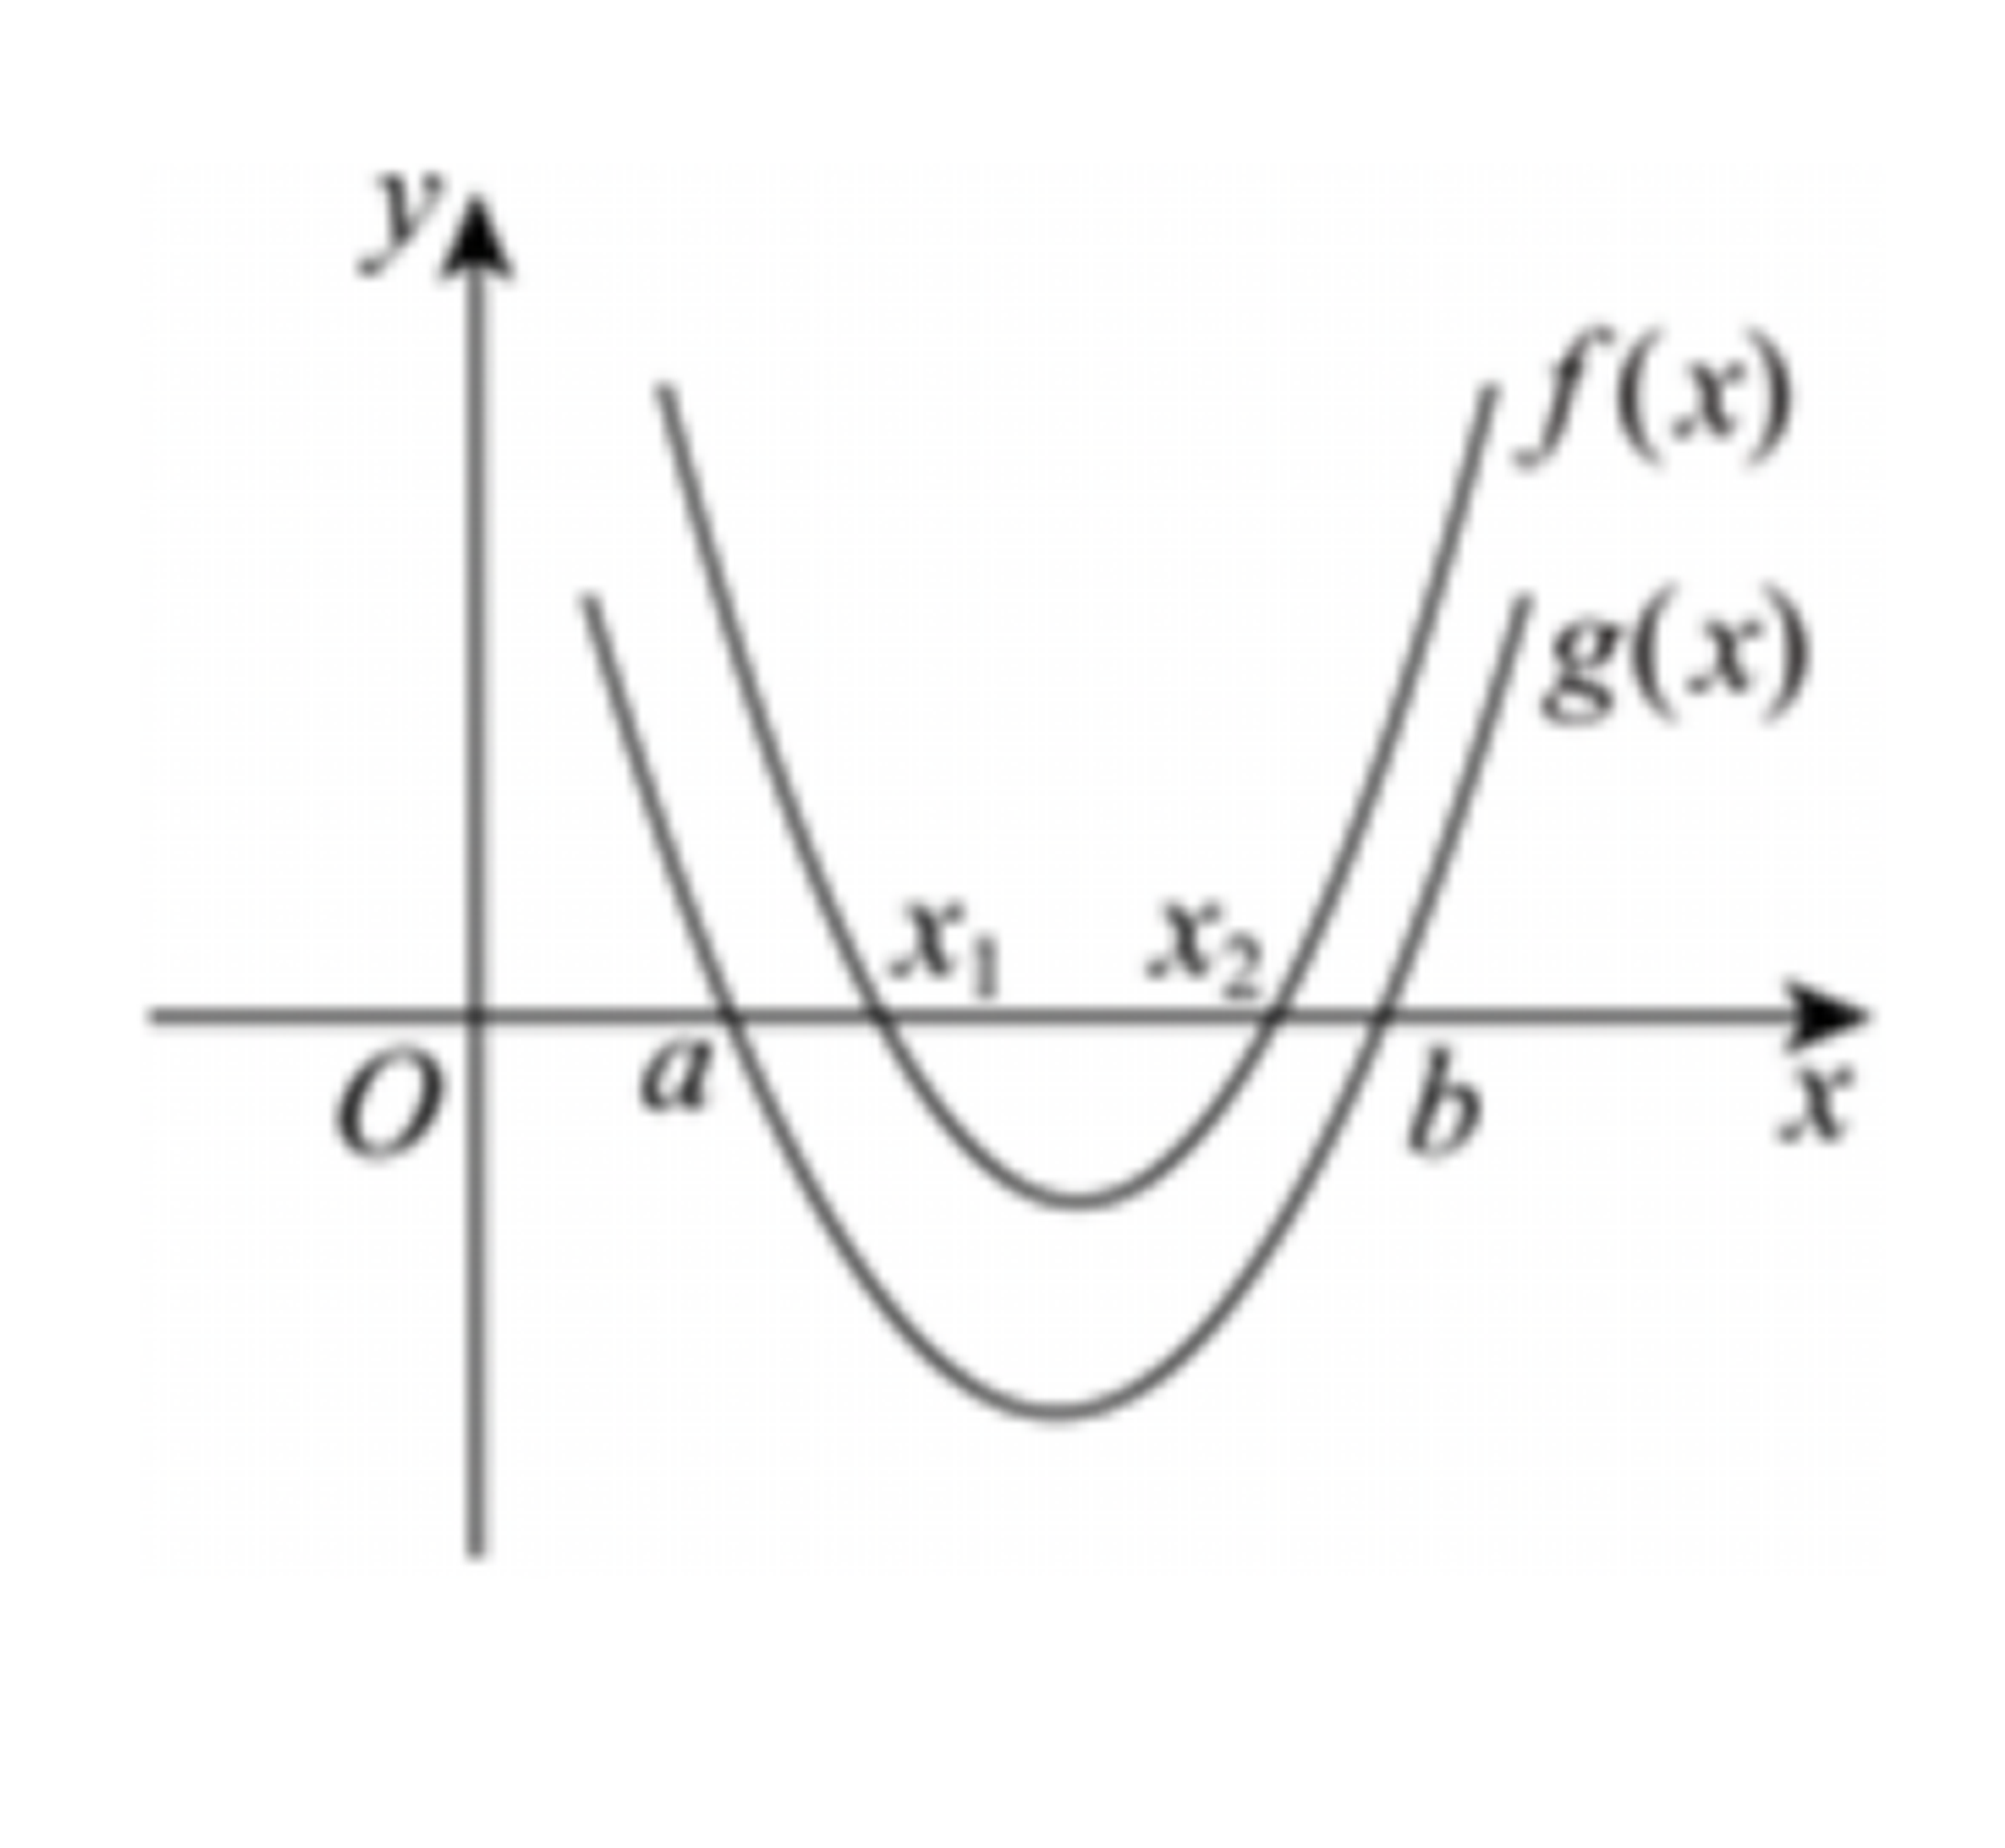
\includegraphics[width=0.30\textwidth]{figures/parabola_f_g_x1x2_h65.png}
\end{center}
\step{由图像得 $a<x_1<x_2<b$，故选 $B$.}
\solend
\fi

\end{enumerate}

\bigsec{三、解答题}

\begin{enumerate}
\setcounter{enumi}{16}

\item 已知 $a>0$，$b>0$，若 $a+b>4$，求证：$\dfrac a{b+2}$ 和 $\dfrac b{a+2}$ 中至少有一个大于 $\dfrac12$.

\ifanswer
\solbegin
\step{假设 $\dfrac a{b+2}\leqslant\dfrac12$，$\dfrac b{a+2}\leqslant\dfrac12$，}
\step{$a>0$，$b>0$，则 $a+2>0$，$b+2>0$，故 $2a\leqslant b+2$，$2b\leqslant a+2$，}
\step{两式相加得 $a+b\leqslant4$，与 $a+b>4$ 矛盾，故 $\dfrac a{b+2}$ 和 $\dfrac b{a+2}$ 中至少有一个大于 $\dfrac12$.}
\solend
\fi

\ansspace[6]

\item 已知集合 $A=\{x\mid-4<x<5\}$，$B=\{x\mid x\leqslant a-6\text{ 或 }x\geqslant a+2\}$.

\begin{enumerate}[label=(\arabic*)]

\item 若 $A\cup B=\R$，求实数 $a$ 的取值范围；

\item 若“$x\in A$”是“$x\in B$”的充分不必要条件，求实数 $a$ 的取值范围.

\end{enumerate}

\ifanswer
\solbegin
\stepm{(1)}{集合 $A=\{x\mid-4<x<5\}$，$B=\{x\mid x\leqslant a-6\text{ 或 }x\geqslant a+2\}$.}
\step{由 $A\cup B=\R$ 得 $\begin{cases}a-6\geqslant-4\\ a+2\leqslant5\end{cases}$，解得 $2\leqslant a\leqslant3$，$a$ 的取值范围为 $[2,3]$；}
\stepm{(2)}{若“$x\in A$”是“$x\in B$”的充分不必要条件，则 $A\subset B$，}
\step{则 $5\leqslant a-6$ 或 $-4\geqslant a+2$，解得 $a\leqslant-6$ 或 $a\geqslant11$.}
\solend
\fi

\ansspace[8]

% 注：原卷题干把命题 $P$ 印作“$\exists3\notin A$”（多一个存在量词），而【解析】两处均作
%     “$3\notin A$”；照录未改，见文件头“原卷笔误/存疑”③。
\item 已知集合 $A=\left\{x\mid\dfrac{x-1}{x-m}<0\right\}$，集合 $B=\left\{x\mid\left|\dfrac{x-1}{x-3}\right|\geqslant1\right\}$，命题 $P$：“$\exists3\notin A$”，命题
$Q$：$A\cap B\neq\varnothing$.

\begin{enumerate}[label=(\arabic*)]

\item 若命题 $P$ 为真命题，求 $m$ 的取值范围；

\item 若命题 $P$ 和命题 $Q$ 至少有一个为假命题，求实数 $m$ 的取值范围.

\end{enumerate}

\ifanswer
\solbegin
\stepm{(1)}{$A=\left\{x\mid\dfrac{x-1}{x-m}<0\right\}=\{x\mid(x-1)(x-m)<0\}$，}
\step{若命题 $P$：“$3\notin A$”为真命题，则 $(3-1)(3-m)\geqslant0$，解得 $m\leqslant3$，}
\step{故实数 $m$ 的取值范围为 $(-\infty,3]$；}
\stepm{(2)}{$B=\left\{x\mid\left|\dfrac{x-1}{x-3}\right|\geqslant1\right\}$，由 $\left|\dfrac{x-1}{x-3}\right|\geqslant1$，得 $\begin{cases}|x-1|\geqslant|x-3|\\ x\neq3\end{cases}$，}
\step{等价于 $\begin{cases}(x-1)^2\geqslant(x-3)^2\\ x\neq3\end{cases}$，解得 $x\geqslant2$ 且 $x\neq3$，所以 $B=[2,3)\cup(3,+\infty)$，}
\step{因为 $A=\{x\mid(x-1)(x-m)<0\}$，}
\step{当 $m=1$ 时，$A=\varnothing$，不满足 $A\cap B\neq\varnothing$，}
\step{当 $m<1$ 时，$A=(m,1)$，不满足 $A\cap B\neq\varnothing$，}
\step{当 $m>1$ 时，$A=(1,m)$，要使 $A\cap B\neq\varnothing$，则 $m>2$，}
\step{则若命题 $Q$：“$A\cap B\neq\varnothing$”为真命题时，实数 $m$ 的取值范围为 $(2,+\infty)$，}
\step{当命题 $P$ 与命题 $Q$ 都是真命题时，则 $\begin{cases}m\leqslant3\\ m>2\end{cases}$，解得 $2<m\leqslant3$，}
\step{则命题 $P$ 和命题 $Q$ 至少有一个为假命题时，得 $m\leqslant2$ 或 $m>3$，}
\step{故实数 $m$ 的取值范围为 $(-\infty,2]\cup(3,+\infty)$.}
\solend
\fi

\ansspace[8]

\item 已知函数 $y=ax^2-(a+2)x+2$，$a\in\R$.

\begin{enumerate}[label=(\arabic*)]

\item $y<3-2x$ 恒成立，求实数 $a$ 的取值范围；

% 注：原卷末句作“求实数 $a$ 的取值”（疑脱“范围”二字），照录未改，
%     见文件头“原卷笔误/存疑”⑤。
\item 若存在 $m>0$ 使关于 $x$ 的方程 $ax^2-(a+2)|x|+2=m+\dfrac1m+1$ 有四个不同的实根，
求实数 $a$ 的取值.

\end{enumerate}

\ifanswer
\solbegin
\stepm{(1)}{由题意得 $ax^2-(a+2)x+2<3-2x$ 恒成立，}
\step{即 $ax^2-ax-1<0$ 恒成立，}
\step{当 $a=0$ 时，$-1<0$ 恒成立，符合题意，}
\step{当 $a\neq0$ 时，则 $\begin{cases}a<0\\ \triangle=a^2+4a<0\end{cases}$，得 $\begin{cases}a<0\\ -4<a<0\end{cases}$，得 $-4<a<0$，}
\step{综上，$a$ 的取值范围为 $(-4,0]$.}
\stepm{(2)}{当 $m>0$ 时，令 $t=m+\dfrac1m+1\geqslant2\sqrt{m\times\dfrac1m}+1=3$，}
\step{当且仅当 $m=1$ 时取等号，}
% 注：题干只给“函数 $y=ax^2-(a+2)x+2$”，全卷未设 $f$，此处 $f(|x|)$ 无定义；
%     照录未改，见文件头“原卷笔误/存疑”④。
\step{则关于 $x$ 的方程 $f(|x|)=t$ 可化为 $a|x|^2-(a+2)|x|+2-t=0$，}
\step{关于 $x$ 的方程为 $a|x|^2-(a+2)|x|+2-t=0$ 有四个不等的实数根，}
\step{即 $ax^2-(a+2)x+2-t=0$，有两个不同的实数正根，}
\step{则 $\begin{cases}\triangle=(a+2)^2-4a(2-t)>0\\ \dfrac{a+2}a>0\\ \dfrac{2-t}a>0\end{cases}$，解得 $a<-2$，}
\step{由（1）得存在 $t\in[3,+\infty)$ 使得不等式 $4at+(a+2)^2-8a>0$ 成立，}
\step{故 $4a\times3+(a+2)^2-8a>0$，即 $a^2+8a+4>0$，}
\step{解得 $a<-4-2\sqrt3$ 或 $a>-4+2\sqrt3$，}
\step{综上，$a<-4-2\sqrt3$，所以 $a$ 的取值范围为 $(-\infty,-4-2\sqrt3)$.}
\solend
\fi

\ansspace[8]

\item 若集合 $A=B_1\cup B_2\cup\cdots\cup B_n$，其中 $B_1$、$B_2$、$\cdots$、$B_n$ 为非空集合，
$B_i\cap B_j=\varnothing$($1\leqslant i<j\leqslant n$)，则称集合 $\{B_1,B_2,\cdots,B_n\}$ 为集合 $A$ 的一个 $n$ 划分.

\begin{enumerate}[label=(\arabic*)]

\item 写出集合 $A=\{1,2,3\}$ 的所有不同的 2 划分；

\item 设 $\{B_1,B_2\}$ 为有理数集 $\Q$ 的一个 2 划分，且满足对任意 $x\in B_1$，任意 $y\in B_2$，都有
$x<y$，判断命题“$B_1$ 中的元素存在最大值，$B_2$ 中的元素存在最小值.”的真假，并说明
理由.

\item 设集合 $A=\{1,2,3,\cdots,16\}$，对于集合 $A$ 的任意一个 3 划分 $\{B_1,B_2,B_3\}$，判断是否存
在 $i\in\{1,2,3\}$，存在 $a$、$b\in B_i$，使得 $b-a\in B_i$ 成立，并说明理由.

\end{enumerate}

\ifanswer
\solbegin
% 注：原卷三个“2 划分”本有外层花括号（$\{\{1,2\},\{3\}\}$ 等），首轮误脱；
%     第二轮复核照原卷补回（原卷原样 / 本稿原错处：原脱外层花括号）。
\stepm{(1)}{集合 $A=\{1,2,3\}$ 的所有不同的 2 划分为 $\{\{1,2\},\{3\}\}$、$\{\{1,3\},\{2\}\}$、}
\step{$\{\{2,3\},\{1\}\}$.}
\stepm{(2)}{该命题为假命题，理由如下：}
\step{假设命题为真，则不妨设 $B_1$ 中元素的最大值为 $s$，$B_2$ 中元素的最小值为 $t$，}
\step{由题意得 $s<t$，所以 $s<\dfrac{s+t}2<t$，}
\step{因为 $s$ 为 $B_1$ 中元素的最大值，所以 $\dfrac{s+t}2\notin B_1$，}
\step{因为 $t$ 为 $B_2$ 中元素的最小值，所以 $\dfrac{s+t}2\notin B_2$，}
\step{因为 $B_1\cup B_2=\Q$，所以 $\dfrac{s+t}2\notin\Q$，}
\step{这与 $\dfrac{s+t}2\in\Q$ 矛盾，所以假设不成立，即命题不可能成立；}
\stepm{(3)}{由于集合 $A$ 中有 16 个元素，}
\step{所以 $B_1$、$B_2$、$B_3$ 中至少有一个集合至少包含 6 个元素，}
\step{不妨设 $B_1$ 中至少包含 6 个元素，}
\step{设 $b_1$、$b_2$、$b_3$、$b_4$、$b_5$、$b_6\in B_1$，且 $b_1<b_2<b_3<b_4<b_5<b_6$，}
\step{假设对任意 $i\in\{1,2,3\}$，对任意 $a$、$b\in B_i$，都有 $b-a\notin B_i$，}
\step{那么 $b_6-b_1$、$b_6-b_2$、$b_6-b_3$、$b_6-b_4$、$b_6-b_5\notin B_1$，}
\step{又因为 $b_6-b_1$、$b_6-b_2$、$b_6-b_3$、$b_6-b_4$、$b_6-b_5\in A$，}
\step{所以 $b_6-b_1$、$b_6-b_2$、$b_6-b_3$、$b_6-b_4$、$b_6-b_5\in B_2\cup B_3$，}
\step{则 $B_2$、$B_3$ 中必有一个集合}
\step{至少包含 $b_6-b_1$、$b_6-b_2$、$b_6-b_3$、$b_6-b_4$、$b_6-b_5$ 中的 3 个元素，}
\step{不妨设这 3 个元素为 $a_1$、$a_2$、$a_3\in B_2$，$a_1<a_2<a_3$，}
\step{由假设得 $a_3-a_1$、$a_3-a_2$、$a_2-a_1\notin B_2$，}
\step{对任意 $i$、$j$($1\leqslant j<i\leqslant3$)，存在 $m$、$n$($1\leqslant m<n\leqslant5$)，}
\step{都有 $a_i-a_j=b_6-b_m-b_6+b_n=b_n-b_m\notin B_1$，}
\step{又因为 $a_3-a_1$、$a_3-a_2$、$a_2-a_1\in B_3$，而 $a_3-a_1-(a_3-a_2)=a_2-a_1$，}
\step{与假设矛盾，所以假设不成立，}
\step{即存在 $i\in\{1,2,3\}$，存在 $a$、$b\in B_i$，使得 $b-a\in B_i$.}
\solend
\fi

\ansspace*[10]

\end{enumerate}

\end{document}
